\chapter{Les subordonnées fragmentaires : les relatives sans verbe} \label{ch3}


La plupart des travaux sur l’ellipse prennent comme contexte privilégié le domaine de la coordination, certaines constructions elliptiques étant considérées comme spécifiques à la coordination (voir, par exemple, des étiquettes comme \is{Conjunction Reduction}\textit{Conjunction Reduction}, cf. \citealt{Jackendoff1971}, ou encore \is{Argument Cluster Coordination (ACC)}\textit{Argument Cluster Coordination}, cf. \citealt{Steedman2000}). Le défi de ce chapitre est de faire sortir l’ellipse du domaine de la coordination, en prenant en compte des subordonnées elliptiques, et en particulier les phrases relatives sans verbe. Je m’appuie ici sur les travaux de \citet{BilbiieEtAl2009,BilbiieEtAl2010}, avec un regard particulier sur les données du roumain et du français.


\section{Qu’est-ce qu’une relative sans verbe?}\label{ch3:sect3.1}

Il existe en roumain et en français des relatives sans verbe (dorénavant RSV), illustrées en \REF{ch3:ex1} et \REF{ch3:ex2}, qui partagent des propriétés formelles avec les phrases relatives verbales. Sur la base de cette ressemblance formelle, ces relatives ont été décrites comme des phrases relatives elliptiques (voir \citealt{Grevisse1993} pour le français, et \citealt{Gheorghe2004}, \citealt{Gheorghe2005} pour le roumain).  

\ea \label{ch3:ex1}
\ea
\gll La  întâlnire  au  venit  trei  persoane,  [\{\textbf{printre}  {\textbar} \textbf{între}\}  \textbf{care} (şi)  Maria].\\
à  rendez-vous \textsc{aux.3pl} venu  trois  personnes  \{parmi  {\textbar}  parmi\}  lesquelles (aussi)  Maria\\ 
\glt ‘Au rendez-vous, trois personnes sont venues, parmi lesquelles Maria.’

\ex
\gll Au  venit  trei  persoane,  [\textbf{dintre} \textbf{care}  una  ieri].\\
\textsc{aux.3pl} venu  trois  personnes  parmi  lesquelles  une  hier\\
\glt ‘Plusieurs personnes sont venues, dont une hier.’
\z
\z


\ea \label{ch3:ex2}
\ea
Trois personnes, [\textbf{parmi lesquelles} Jean], sont venues.
\ex
Trois personnes sont venues [\textbf{dont} une hier].
\z
\z

On trouve aussi ces relatives sans verbe dans d’autres \ili{langues romanes}, comme \il{italien}l’italien \REF{ch3:ex3} ou \il{espagnol}l’espagnol \REF{ch3:ex4}:


\ea\label{ch3:ex3}
 
\ea
Quattro persone sono state arrestate, [\{\textbf{tra} {\textbar} \textbf{fra} {\textbar} *\textbf{di}\} \textbf{cui} Maria]\footnote{L’agrammaticalité de la préposition \textit{di} dans cet exemple est due à la sémantique de cette préposition, qui est incompatible avec une \isi{interprétation exemplifiante}, comme on verra dans la section~\ref{ch3:sect3.3.2.2}.}. \\
\glt ‘Quatre personnes ont été arrêtées, parmi lesquelles Maria.’

\ex
Quattro persone sono state arrestate, [\{\textbf{tra} {\textbar} \textbf{fra} {\textbar} \textbf{di}\} \textbf{cui} due ieri].\\
\glt ‘Quatre personnes ont été arrêtées, parmi lesquelles deux hier.’

\ex
Queste spiagge offrono rifugio a molte specie d’animali, [\textbf{fra} \textbf{queste}, in particolare, (a) degli orsetti].\\
\glt ‘Ces plages offrent un refuge à plusieurs espèces d’animaux, parmi lesquelles, en particulier, (à) des oursons.’
\z
\z


\ea \label{ch3:ex4}
\ea
\gll En  esta  foto,  puedes  ver  varias  casas,  [\textbf{entre} \textbf{las} \textbf{cuales} la  nuestra].\\
dans  cette  photo  pouvoir.\textsc{prs.2sg}  voir  variées  maisons  parmi  les  quelles la  nôtre\\ 
\glt ‘Sur cette photo, tu peux voir différentes maisons, parmi lesquelles la nôtre.’

\ex
\gll Los  doce  están  presentes,  [dos  \textbf{de} \textbf{los} \textbf{cuales}  representados  por  sus presidentes].\\
les  douze  sont  présents  deux  de  les  quels  représentés  par  \textsc{poss} président\\
\glt ‘Les douze sont présents, dont deux représentés par leur président.’ 
\z
\z

Le domaine empirique de la construction qui nous intéresse ici est le suivant : une relative sans verbe (RSV) est un syntagme caractérisé par un constituant initial qui est soit un syntagme prépositionnel contenant une forme \textit{qu-} (roum. \textit{printre} \textbf{\textit{care}}, \textit{între} \textbf{\textit{care}}, \textit{dintre} \textbf{\textit{care}} ; fr. \textit{parmi} \textbf{\textit{lesquel(le)s}}), soit la forme \textit{dont} en français. Le syntagme initial est suivi d’un ou de plusieurs constituants sans qu’il y ait de verbe fini. Cette définition du domaine empirique exclut toute phrase relative complète (verbale et finie), comme en \REF{ch3:ex5} et \REF{ch3:ex6}.

\ea \label{ch3:ex5}
\ea
Autobuzul cu refugiaţi, [\textbf{printre} \textbf{care} se aflau şi patru români]\textsubscript{REL}, a fost întors în Gaza, din motive de securitate. \\
\glt ‘Le bus avec des réfugiés, parmi lesquels il y avait aussi quatre Roumains, a été renvoyé à Gaza, pour des raisons de sécurité.’
\ex
Datele statistice arată că în acest oraş lucrează aproximativ 160~000 de persoane, [\emph{\textbf{\textup{dintre}}}\emph{\textbf{} }\emph{\textbf{\textup{care}}} aproape 130~000 activează în domeniul privat]\textsubscript{REL}.\\
\glt ‘Les données statistiques montrent que dans cette ville travaillent environ 160~000 personnes, parmi lesquelles presque 130~000 ont une activité dans le secteur privé.’
\z
\z

\ea \label{ch3:ex6} 
\ea
Le recrutement a repris : 3~500 personnes [\textbf{dont} près de 800 cadres ont été embauchés  à l’extérieur de FranceTélécom]\textsubscript{REL}.
\ex 
Il a écrit plusieurs romans, [\textbf{dont} deux ont été publiés le mois dernier]\textsubscript{REL}.
\z
\z

Ce chapitre consacré à l’analyse des RSV développe en particulier les aspects suivants. Premièrement, je montre que les propriétés syntaxiques et sémantiques des RSV sont très différentes de celles des phrases relatives. Une analyse qui tente de réduire les RSV à des phrases elliptiques dérivées des phrases relatives ordinaires ne permet pas de rendre compte de ces différences. Deuxièmement, les RSV sont des fragments qui peuvent contenir des \is{cluster}clusters de constituants. Troisièmement, les RSV peuvent avoir deux types de sémantique : une \isi{interprétation exemplifiante} ou bien une \isi{interprétation partitionnante}.

Afin de faciliter la lecture, j’utilise la terminologie suivante : j’appelle \textit{hôte} (ou \textit{source}\footnote{Cependant, les termes de \textit{hôte} et \textit{source} ne sont pas utilisés ici en variation libre, mais en fonction de la perspective qu’on a sur le RSV : si on parle d’une RSV en termes purement syntaxiques comme étant un \isi{ajout incident} (voir la section~\ref{ch3:sect3.2.3} ci-dessous), la phrase le contenant est l’hôte ; en revanche, si on parle d’une RSV en termes plutôt sémantiques comme étant un \isi{fragment} (dont l’interprétation n’est pas autonome), la phrase qui offre le matériel nécessaire à l’interprétation est étiquetée comme source.}) la phrase ou l’énoncé contenant directement ou non la RSV \REF{ch3:ex7a} ; la RSV est composée d’un \textit{introducteur} et d’un \textit{corps} \REF{ch3:ex7b}. Les RSV introduisent toujours une relation partitive entre une expression de leur hôte (appelée \textit{antécédent} ou \textit{légitimeur}) et une expression de leur corps (appelé \textit{élément distingué}), cf. \REF{ch3:ex7c}.

\ea \label{ch3:ex7}
\ea {}
\gll [Au venit  trei  persoane]\textit{\textsubscript{Hôte}}, [\textbf{dintre} \textbf{care}  una  ieri]\textsubscript{RSV}. \label{ch3:ex7a}\\
\textsc{aux.3pl} venu  trois  personnes  parmi  lesquelles  une  hier\\
\glt ‘Plusieurs personnes sont venues, dont une hier.’
\ex
Au venit trei persoane, [[dintre care]\textit{\textsubscript{Introducteur}} [una ieri]\textit{\textsubscript{Corps}}]. \label{ch3:ex7b}
\ex
Au venit [trei persoane]\textit{\textsubscript{Antécédent}}, dintre care [una]\textit{\textsubscript{Elément distingué}} ieri. \label{ch3:ex7c}
\z
\z

Les résultats de cette étude se basent essentiellement sur des exemples attestés. Pour le français, une partie des données utilisées dans cet ouvrage provient du Corpus Arboré de Paris 7 \citep{AbeilleEtAl2003b}. Le corpus est composé d’extraits du journal \textit{Le Monde} (de 1989 à 1993). Il contient 138 instances de RSV sur 21~560 segments tagués comme «~phrases relatives~». Quant aux données du roumain, elles proviennent en grande partie de textes de presse, étant donné l’inexistence d’un corpus similaire en roumain. J’ai recueilli 202 occurrences, dont 81 avec l’introducteur \textit{dintre care}, 63 avec l’introducteur \textit{între care} et 58 avec \textit{printre care}. En français, on observe une forte asymétrie entre le nombre d’instances faisant intervenir l’introducteur \textit{dont} (127 occurrences) et celles faisant intervenir un introducteur prépositionnel avec une forme \textit{qu-} (11 occurrences). Cette asymétrie est peut-être liée au fait que la syntaxe et la sémantique des RSV avec \textit{dont} en français sont moins contraintes que celles faisant intervenir des syntagmes prépositionnels avec une forme \textit{qu-}. En revanche, les données du roumain ne disent a priori rien sur la fréquence des trois syntagmes prépositionnels dans l’usage contemporain\footnote{Comme le note Olivier Bonami (c.p.), la différence pourrait aussi être due au mode de constitution très différent du corpus, voire aux conventions d’annotation du Corpus Arboré de Paris~7.}.


\section{Propriétés syntaxiques}\label{ch3:sect3.2}

Dans cette section, je m’intéresse à la constituance des RSV, en regardant les propriétés distributionnelles de l’introducteur et du corps d’une RSV. En particulier, il s’agit de voir si l’introducteur \textit{dont} dans les RSV est le même que le complémenteur \textit{dont} dans les phrases relatives ordinaires. Je présente ensuite les modalités de constitution pour le corps d’une RSV (le corps contient-il uniquement l’élément distingué ou d’autres constituants immédiats~?). Parallèlement à cela, je regarde si l’élément distingué dans le corps d’une RSV permet le même marquage (\is{marquage prépositionnel}prépositionnel ou \is{marquage casuel}casuel) que l’antécédent dans la phrase hôte. Enfin, j’étudie les propriétés de \isi{linéarisation} des RSV par rapport à l’antécédent, pour voir s’il s’agit d’une adjacence stricte ou non.


\subsection{L’introducteur d’une RSV}\label{ch3:sect3.2.1}

En roumain, l’introducteur d’une RSV est toujours un syntagme prépositionnel contenant une préposition et une forme \textit{qu-} ; en français, on trouve le plus souvent la forme \textit{dont}, mais aussi des syntagmes prépositionnels.

L’introducteur d’une RSV, comme l’indique son nom, précède toujours le corps de la RSV (\ref{ch3:ex8}--\ref{ch3:ex9}), tout comme les syntagmes extraits ou les complémenteurs dans les phrases relatives ordinaires.

\ea \label{ch3:ex8}
\ea
\gll Mai  multe  ţări  sud-americane,  [\textbf{printre} \textbf{care} şi  Brazilia], exportă  cafea  în  Europa. \\
plus  beaucoup.\textsc{adj}  pays  sud-américains  parmi  lesquels  aussi  Brésil.\textsc{def} exportent  café  en  Europe.\textsc{def}\\
\glt ‘Plusieurs pays sud-américains, parmi lesquels le Brésil, exportent du café en Europe.’

\ex
\gll *Mai  multe  ţări  sud-americane,  [şi  Brazilia \textbf{printre} \textbf{care}], exportă  cafea  în  Europa. \\
plus  beaucoup.\textsc{adj}  pays  sud-américains  aussi  Brésil.\textsc{def}  parmi  lesquels exportent  café  en  Europe.\textsc{def}\\
\z
\z

\ea \label{ch3:ex9}
\ea Plusieurs personnes sont venues, [\{\textbf{parmi lesquelles {\textbar} dont}\} Jean].
\ex *Plusieurs personnes sont venues, [Jean \{\textbf{parmi lesquelles {\textbar} dont}\}].
\z
\z

Le début de l’introducteur d’une RSV coïncide avec le début de la RSV, ce qui explique l’impossibilité d’avoir un introducteur précédé par un adverbial comme le roumain \textit{în mod special} ‘en particulier’ en \REF{ch3:ex10b} ou le français \textit{notamment} en \REF{ch3:ex11b}.  

\ea \label{ch3:ex10}
\ea
\gll Mai  multe  ţări,  [\textbf{printre} \textbf{care} \ulg{în}{23}  mod  special  Brazilia], exportă  cafea  în  Europa. \label{ch3:ex10a}\\
plus  beaucoup.\textsc{adj} pays  parmi  lesquels  en  mode  spécial  Brésil.\textsc{def} exportent  café  en  Europe.\textsc{def}\\
\glt ‘Plusieurs pays, parmi lesquels en particulier le Brésil, exportent du café en Europe.’

\ex 
\gll *Mai  multe  ţări,  [\ulg{în}{23}  mod  special  \textbf{printre} \textbf{care}  Brazilia], exportă  cafea  în  Europa. \label{ch3:ex10b}\\
plus  beaucoup.\textsc{adj}  pays  en  mode  spécial  parmi lesquels  Brésil.\textsc{def} exportent  café  en  Europe.\textsc{def}\\
\z
\z

\ea \label{ch3:ex11}
\ea Plusieurs personnes sont venues, [\{\textbf{parmi lesquelles {\textbar} dont}\} \uline{notamment} Jean]. \label{ch3:ex11a}
\ex *Plusieurs personnes sont venues, [\uline{notamment} \{\textbf{parmi lesquelles {\textbar} dont}\} Jean]. \label{ch3:ex11b}
\z
\z

Par la suite, je m’intéresse à la distribution des introducteurs des RSV, en discutant séparément les syntagmes prépositionnels contenant une forme \textit{qu-} dans les deux langues et la forme \textit{dont} en français. Il est bien admis que les relatives mettent en jeu une diversité syntaxique impressionnante \citep{Godard1988,AbeilleEtAl2006} et qu’elles peuvent être introduites par un syntagme contenant un pronom relatif ou bien par un complémenteur.

Les critères définitoires pour la distinction entre pronom relatif et complémenteur retenus par \citet{AbeilleEtAl2006} sont les suivants : (i) au niveau morphologique, seuls les pronoms peuvent varier en genre et en nombre ; (ii) au niveau sémantique, seuls les pronoms ont un indice référentiel, leur permettant de contraindre leur antécédent (p.ex. à dénoter un être animé) ; (iii) seuls les complémenteurs contraignent le mode de la phrase qu’ils introduisent ; (iv) seuls les pronoms peuvent être complément d’une préposition. Sur la base de ces propriétés, on doit décider si les introducteurs des RSV, les formes \textit{qu-} d’un côté et la forme \textit{dont} de l’autre, ont tous la même catégorie.  


\subsubsection{Syntagmes prépositionnels}\label{ch3:sect3.2.1.1}

En dehors des trois syntagmes prépositionnels du roumain\textit{ printre care, între care} et \textit{dintre}\footnote{En roumain non standard, on utilise la préposition \textit{din} à la place de la préposition \textit{dintre}. Dans cet ouvrage, je laisse de côté ces exemples. Voir aussi la note \ref{ch3:fn11} ci-dessous.}\textit{care} et le syntagme prépositionnel \textit{parmi lesquel(le)s} en français, on trouve d’autres expressions exprimant l’appartenance à un ensemble, avec éventuellement un ordre d’importance au sein de cet ensemble : on a ainsi en roumain des formes telles que \textit{în rândul cărora} ‘au rang desquels’ (illustrée en \REF{ch3:ex12}), \textit{în mij\-locul cărora} ‘au milieu desquels’, \textit{în fruntea cărora} ‘au sommet desquels’ et en français des formes comme \textit{au nombre desquels} (illustrée en \REF{ch3:ex13a})\textit{, au} \{\textit{sein {\textbar} centre}\}\textit{ desquels, au sommet desquels, au} \{\textit{premier {\textbar} second}\} \textit{rang} \textit{desquels}. En français, on enregistre aussi le syntagme nominal complexe\textit{ parmi les plus important(e)s desquel(le)s}, qui est assez rare, mais possible dans la mesure où la relation partitive entre l’antécédent et l’élément distingué subsiste \REF{ch3:ex13b}. Ces expressions, qui habituellement dénotent des relations spatiales en dehors de leur emploi dans les RSV, sont toujours utilisées avec un sens partitif abstrait dans les RSV, ce qui explique l’agrammaticalité des exemples en \REF{ch3:ex14} et \REF{ch3:ex15}.  

\ea \label{ch3:ex12}
\gll Un  număr  de  zece  state,  [\textbf{în} \textbf{rândul} \textbf{cărora} şi  România],  au  semnat un  acord  cu  ONU  privind  ajutorarea  refugiaţilor.\\
un  nombre  de  dix  états  en  rang.\textsc{def}  desquels  aussi  Roumanie.\textsc{def}  ont  signé un  accord  avec  ONU  concernant  secours.\textsc{def}  réfugiés.\textsc{gen} \\
\glt ‘Un nombre de dix états, au nombre desquels la Roumanie, ont signé un accord avec l’ONU concernant le secours des réfugiés.’ 
\z

\ea \label{ch3:ex13}
\ea
Les paysages urbains et la vie en ville dépendent de multiples facteurs, [\textbf{au nombre desquels} la culture et l’histoire, le cadre naturel, les activités, la situation démographique et le niveau de développement]. \label{ch3:ex13a}
\ex
Par contre, le recul perçu, ce que ressent le tireur, est une chose éminemment subjective qui est influencée par différents facteurs, [\textbf{parmi les plus importants desquels} la forme et l’ajustement de la crosse]. \label{ch3:ex13b}
\z
\z

\ea\label{ch3:ex14}
\gll *Am  amenajat  mai  multe  camere,  [\textbf{în} \textbf{mijlocul} \textbf{cărora} câte o masă].\\
avons  aménagé  plus  beaucoup.\textsc{adj}  chambres  en  milieu.\textsc{def} desquelles \textsc{distr} une  table\\
\glt ‘On a aménagé plusieurs chambres et on a mis une table au milieu de chacune d’entre elles.’
\z

\ea\label{ch3:ex15}
 *La montagne, [\textbf{au sommet de laquelle} Jean], s’appelle le Cervin.
\z

Les syntagmes prépositionnels que je retiens dans ce chapitre contiennent une préposition (roum. \textit{printre, între} ou \textit{dintre} et fr. \textit{parmi}) et une forme \textit{qu-} qui est un élément \is{anaphore}anaphorique dont l’antécédent se trouve dans la phrase hôte. La forme \textit{qu-} est donc coréférente avec l’antécédent dans la phrase hôte, ce qui est signalé par \is{accord}l’accord morphologique de la forme \textit{qu-} avec l’antécédent en nombre (toujours pluriel : fr. \textit{lesquels {\textbar} desquels}) et en genre (cf. en français, la distinction masculin \textit{lesquels {\textbar} desquels} vs. féminin \textit{lesquelles {\textbar} desquelles}). En roumain, \is{accord}l’accord en nombre n’est pas «~visible~» avec la forme nominative-accusative \textit{care} (qui présente la même forme au singulier et au pluriel), mais il est observé avec la forme dative-génitive au pluriel \textit{cărora} en \REF{ch3:ex12}. En revanche, aucune de ces deux formes ne permet de distinction en fonction du genre.


On observe donc que les formes \textit{qu-} \textit{lesquel(le)s} en français et \textit{care} en roumain satisfont le premier critère (mentionné plus haut) attribué aux pronoms relatifs, à savoir elles sont des formes fléchies. De plus, les formes \textit{qu-} que l’on retrouve dans les RSV sont toujours des compléments de préposition : en français, \textit{lesquel(le)s} est le complément de la préposition \textit{parmi}~; en roumain \textit{care} est le complément de la préposition \textit{printre, între} ou \textit{dintre}. Sur la base de ces deux propriétés, on peut analyser les formes \textit{qu-} comme des pronoms relatifs.  


\subsubsection{La forme \textit{dont} en français}\label{ch3:sect3.2.1.2}

En dehors de son usage dans les RSV, la forme \textit{dont} en français n’apparaît qu’à l’initiale de phrases relatives (y compris coda de \isi{clivée} et de \isi{pseudoclivée}). Dans les relatives ordinaires, cette forme est analysée comme un complémenteur et non comme une forme \textit{qu-} prépositionnelle \citep{Godard1988,Godard1989,AbeilleEtAl2003c,AbeilleEtAl2006,AbeilleEtAl2007}, sur la base des propriétés suivantes. Premièrement, \textit{dont} dans les phrases relatives ordinaires contraint le mode de la relative ; il se combine uniquement avec des phrases finies (\ref{ch3:ex16a}--\ref{ch3:ex16b}), alors que les relatives introduites par une forme \textit{qu-} ne sont pas toujours finies \REF{ch3:ex16c}. Deuxièmement, la forme \textit{dont} ne peut être employée comme complément de nom \REF{ch3:ex17a} ou de préposition \REF{ch3:ex17c} dans un syntagme extrait complexe, contrairement à ce qui se passe avec une forme \textit{qu-} en \REF{ch3:ex17b} et \REF{ch3:ex17d}. Troisièmement, le complémenteur \textit{dont} introduit~: (i) soit des phrases relatives contenant un constituant manquant (\textit{gap}) marqué par la forme \textit{de} (voir dans ce sens le contraste entre l’exemple \REF{ch3:ex18a} et \REF{ch3:ex18c}), (ii) soit des relatives contenant un pronom coréférent avec l’antécédent (\isi{pronom résomptif}), à condition qu’il soit enchâssé sous un \isi{prédicat d'attitude propositionnelle}, comme en \REF{ch3:ex19a}~; on explique ainsi l’agrammaticalité de l’exemple \REF{ch3:ex19b} par le fait qu’il manque un \isi{pronom résomptif} approprié, alors que l’inacceptabilité de l’exemple \REF{ch3:ex19c} est due à la présence du prédicat \textit{n’ont pas empêché} à la place d’une \is{prédicat d'attitude propositionnelle}expression d’attitude propositionnelle. Quatrièmement, on peut ajouter l’absence de variation en genre et en nombre pour la forme \textit{dont}, contrairement à des formes \textit{qu-} fléchies (p.ex. \textit{duquel} {\textbar} \textit{de laquelle {\textbar} desquels {\textbar} desquelles})\footnote{J’ajoute ici le fait que, contrairement à des formes \textit{qu-} comme \textit{duquel}, le complémenteur \textit{dont} peut être immédiatement suivi des syntagmes disloqués \REF{ch3:fn5i} ou des ajouts initiaux \REF{ch3:fn5ii}. Selon Olivier Bonami (c.p.), cet effet pourrait être dû à un conflit de registre sociolinguistique entre l’emploi de \textit{duquel} (qui apparaît plutôt dans le registre formel) et la présence d’un disloqué ou d’un ajout en début d’enchâssée (qui relève plutôt du registre informel).

\ea \label{ch3:fn5i}
Je connais quelqu’un [\textbf{dont} \uline{le numéro}, il commence par 04].
\z 

\ea \label{ch3:fn5ii} 
Je cherche le titre d’une chanson [\textbf{dont} \uline{à un endroit des paroles}, ça dit : «~T’as pas été invité sur le plateau de la méthode Cauet~» ou un truc comme ça], c’est du rock.
\z 
}.


\ea \label{ch3:ex16}
\ea
C’est bien de faire sourire la personne [\{\textbf{dont {\textbar} de laquelle}\} on est amoureux]. \label{ch3:ex16a}
\ex 
*Voici un livre [\textbf{dont} parler à nos enfants]. \label{ch3:ex16b}
\ex 
Voici un nouveau produit [\textbf{duquel} parler sur nos blogs]. \label{ch3:ex16c}
\z
\z

\ea \label{ch3:ex17}
\ea
*Paul, 19 ans, [\textbf{contre le frère dont} le procureur avait requis 8 à 10 ans de prison], a tenté de forcer le dispositif de sécurité. \label{ch3:ex17a}
\ex
Paul, 19 ans, [\textbf{contre le frère duquel} le procureur avait requis 8 à 10 ans de prison], a tenté de forcer le dispositif de sécurité. \label{ch3:ex17b}
\ex 
*Mon directeur est une personne [\textbf{près dont} on se sent bien]. \label{ch3:ex17c}
\ex 
Mon directeur est une personne [\textbf{près de laquelle} on se sent bien]. \label{ch3:ex17d}
\z 
\z 

\ea \label{ch3:ex18}
\ea
Voici un poème [\textbf{dont} je me souviens]. \label{ch3:ex18a}
\ex 
Je me souviens \textbf{de} ce poème. \label{ch3:ex18b}
\ex 
*Voici un roman [\textbf{dont} je relis régulièrement]. \label{ch3:ex18c}
\ex 
Je relis ce roman régulièrement. \label{ch3:ex18d}
\z 
\z 

\ea \label{ch3:ex19}
\ea
Voici un livre\textsubscript{i} [\textbf{dont} \uline{il est évident} qu’il\textsubscript{i} coûte cher]. \label{ch3:ex19a}
\ex 
*C’est une question [\textbf{dont} \uline{il est évident} que nous aurons quelques problèmes]. \label{ch3:ex19b}
\ex 
??... un tremblement\textsubscript{i} de terre [\textbf{dont} les nouvelles normes de construction \uline{n’ont pas empêché} qu’il\textsubscript{i} fasse des ravages]. \label{ch3:ex19c}
\z 
\z 

La forme \textit{dont} dans les RSV semble partager une partie des propriétés observées ci-dessus pour le complémenteur \textit{dont} dans les relatives ordinaires. En particulier, elle ne peut pas être enchâssée dans un introducteur complexe \REF{ch3:ex20a}, contrairement au comportement d’une forme \textit{qu-} \REF{ch3:ex20b} dans les RSV.

\ea \label{ch3:ex20}
\ea
*On a auditionné plusieurs candidats, [\textbf{parmi les plus importants dont} Jean Pataut]. \label{ch3:ex20a}
\ex
On a auditionné plusieurs candidats, [\textbf{parmi les plus importants desquels} Jean Pataut]. \label{ch3:ex20b}
\z 
\z 

Cependant, il n’est pas clair que toutes les propriétés de sélection du complémenteur \textit{dont} dans les relatives ordinaires s’appliquent aussi à la forme \textit{dont} dans les RSV. En particulier, si l’on suppose que le complémenteur \textit{dont} dans les relatives ordinaires n’a pas de contribution sémantique, on ne peut pas maintenir cette affirmation dans les RSV, car \textit{dont} dans ces contextes force une interprétation partitive (cf. section~\ref{ch3:sect3.3.2}), {\cad} l’élément distingué dans une RSV doit être une sous-partie de l’ensemble dénoté par l’antécédent dans la phrase hôte (voir le contraste en (\ref{ch3:ex21a}--\ref{ch3:ex21b})).  

\ea \label{ch3:ex21}
\ea
Au total, dix livres ont été commandés, [(*\textbf{dont}) tous pour toi]. \label{ch3:ex21a}
\ex
Au total, dix livres ont été commandés, [(\textbf{dont}) deux pour toi]. \label{ch3:ex21b}
\z 
\z 

De plus, la forme \textit{dont} n’a pas le même comportement distributionnel par rapport à la coordination dans les deux contextes. Si les relatives ordinaires autorisent la répétition de \textit{dont} devant chaque phrase coordonnée \REF{ch3:ex22a}, cela n’est pas autorisé dans la coordination de RSV \REF{ch3:ex22b}. De ce point de vue, la forme \textit{dont} dans les RSV se rapproche des conjonctions (de coordination), dont une des propriétés prototypiques est de ne pas pouvoir se combiner entre elles. En dépit de cette ressemblance, une étude détaillée reste à faire pour voir si la forme \textit{dont} dans les RSV peut être analysée comme conjonction\footnote{La forme \textit{dont} dans les RSV peut encore être rapprochée des items comme \textit{y compris}, \textit{sauf} ou \textit{excepté} (pouvant être considérés comme des prépositions~« a-sélectives~», cf. \citealt{Melis2001}, qui ne sélectionnent pas la catégorie de leur complément). On doit cependant préciser qu’il y a des différences notables entre \textit{dont} des RSV et \textit{y compris} par exemple : \REF{ch3:fn6i} \textit{y compris} est plus mobile que \textit{dont~}; \REF{ch3:fn6ii} l’élément distingué dénotant la sous-partie peut être absent dans le modifieur partitif introduit par \textit{y compris}, et \REF{ch3:fn6iii} la \isi{méronymie} est possible avec \textit{y compris} (cf. \citealt{Laurens2007}). 

\ea \label{ch3:fn6i}
\ea
Plusieurs personnes sont venues, \{\textbf{y compris} Marie {\textbar} Marie \textbf{y compris}\}.
\ex 
Plusieurs personnes sont venues, \{\textbf{dont} Marie {\textbar} *Marie \textbf{dont}\}.
\z 
\z 

\ea \label{ch3:fn6ii}
Il a vendu beaucoup de livres, \{\textbf{y compris} {\textbar} *\textbf{dont}\} sur la plage.
\z 

\ea \label{ch3:fn6iii}
Il aime les suédoises, \{\textbf{y compris} {\textbar} *\textbf{dont}\} leurs cheveux.
\z 
}. 


\ea \label{ch3:ex22}
\ea
Tous mes amis [\textbf{dont} je t’ai parlé \uline{et} \textbf{dont} on a discuté toute la journée] sont morts. \label{ch3:ex22a}
\ex
*Tous mes amis, [\textbf{dont} Marie \uline{et} \textbf{dont} Pierre], sont venus à la fête. \label{ch3:ex22b}
\z 
\z

Un argument supplémentaire contre l’analyse de \textit{dont} comme complémenteur dans les RSV vient de la possibilité de se combiner avec une phrase subordonnée introduite par le complémenteur \textit{que}, comme on voit en \REF{ch3:ex23} :

\ea \label{ch3:ex23}
Sur le site de Porsche, on apprend plusieurs choses, [\textbf{dont} notamment [\uline{que} la compagnie offre ses propres formations spécialisées pour les diplômés et professionnels de l’ingénierie]\textsubscript{S}].
\z

Enfin, comme je le montre dans la section~\ref{ch3:sect3.4}, une analyse qui dérive les RSV des relatives verbales ordinaires n’est pas empiriquement adéquate, donc rien ne nous empêche de poser deux \textit{dont} différents en français : un complémenteur \textit{dont} qui introduit les relatives verbales ordinaires et un \textit{dont} qui introduit les RSV.


\subsection{Le corps d’une RSV}\label{ch3:sect3.2.2}

La constitution du corps d’une RSV se présente sous deux formes : (i) soit un seul constituant, (ii) soit plusieurs constituants formant un cluster, {\cad} un type de syntagme sans tête explicite, contenant une suite de constituants qui ne sont pas liés entre eux par des relations fonctionnelles.


\subsubsection{Un seul constituant}\label{ch3:sect3.2.2.1}

Dans le premier cas de figure, l’élément distingué est le seul constituant du corps. Il peut être un syntagme nominal non marqué ({\cad} un syntagme sans \isi{marquage prépositionnel} en français et en roumain, ou bien un syntagme sans \isi{marquage casuel} spécifique en roumain) ou bien un syntagme de toute catégorie, parallèle à son légitimeur dans la phrase hôte, donc un syntagme qui reçoit un \isi{marquage casuel} (en roumain) ou \isi{marquage prépositionnel}.

Toutes les RSV ne permettent pas les deux options. On observe des asymétries entre le roumain et le français, mais aussi à l’intérieur d’une même langue.~

En français : de manière générale, si on a un seul élément distingué, il ne peut pas recevoir le \isi{marquage prépositionnel} ; par conséquent, on ne peut pas avoir la préposition \textit{à} dans la RSV introduite par \textit{parmi lesquelles} en \REF{ch3:ex24a} ou bien la préposition \textit{avec} dans la RSV introduite par \textit{dont} en \REF{ch3:ex24b}. Cependant, on doit noter qu’en dehors du Corpus Arboré de Paris 7 on trouve des exemples attestés dans lesquels les RSV introduites par \textit{dont} permettent un élément distingué marqué par une préposition, mais avec une acceptabilité variable selon les locuteurs. L’acceptabilité du marquage quand on utilise la forme \textit{dont} peut être améliorée si on ajoute un adverbe comme \textit{notamment} \REF{ch3:ex24c}.

\ea \label{ch3:ex24}
\ea
J’ai parlé \uline{à} plusieurs personnes, [\textbf{parmi lesquelles} (*\uline{à}) Marie]. \label{ch3:ex24a}
\ex
J’ai parlé \uline{avec} certaines personnes, [\textbf{dont} (*\uline{avec}) Marie]. \label{ch3:ex24b}
\ex
Un jeune homme annonce \uline{à} divers protagonistes sa mort prochaine, [\{*\textbf{parmi lesquels} {\textbar} \%\textbf{dont}\} notamment \uline{à} un psychiatre qui se sent dans l’obligation de l’aider]. \label{ch3:ex24c} 
\z 
\z 

En roumain : les introducteurs \textit{printre care} et \textit{între care}\footnote{Il n’y a a priori aucune différence majeure entre \textit{printre care} et \textit{între care}. C’est pour cela que je garde dans mes exemples une des deux formes, à savoir \textit{printre care}.} ne posent aucun problème pour le \isi{marquage casuel} \REF{ch3:ex25a} ou \is{marquage prépositionnel}prépositionnel \REF{ch3:ex25b} de l’élément distingué, pourvu que celui-ci soit précédé de \is{adverbe associatif}l’adverbe associatif \textit{şi} ‘aussi’. En revanche, \textit{dintre care} est généralement incompatible avec une \is{marquage casuel}marque casuelle \REF{ch3:ex26a} ou \is{marquage prépositionnel}prépositionnelle \REF{ch3:ex26b}, à moins que l’élément distingué soit précédé, comme dans le cas du français \textit{dont}, des modifieurs \is{éventualité}d’éventualité\footnote{D’autres auteurs utilisent la notion de \textit{situation}. Je préfère l’emploi de la notion \is{éventualité}d’\textit{éventualité}.}, comme l’adverbial \textit{mai ales} ‘notamment’ \REF{ch3:ex26c}.

\ea \label{ch3:ex25}
\ea
\gll Ion  a  oferit  flori  mai  mult\uline{or} fete,  [\textbf{printre} \textbf{care}  şi \{Maria {\textbar} Mari\uline{ei}\}]. \label{ch3:ex25a}\\
Ion  a  offert  fleurs  plus  beaucoup.\textsc{adj.dat}  filles parmi  lesquelles  aussi \{Maria {\textbar} Maria.\textsc{dat}\}  \\
\glt ‘Ion a offert des fleurs à plusieurs filles, parmi lesquelles Maria.’ 
\ex 
\gll Ion  a  vorbit \uline{cu} mai  multe  fete,  [\textbf{printre} \textbf{care} şi  (\uline{cu}) Maria]. \label{ch3:ex25b}\\
Ion  a  parlé  avec  plus  beaucoup.\textsc{adj}  filles  parmi lesquelles  aussi  (avec) Maria\\
\glt ‘Ion a parlé avec plusieurs filles, parmi lesquelles Maria.’
\z 
\z 

\ea \label{ch3:ex26}
\ea
\gll Impactul  a  dus  la  spitalizarea  mai  multor  persoane, \ [\textbf{dintre} \textbf{care}  (*\uline{a})  şapte  români]. \label{ch3:ex26a}\\
impact.\textsc{def}  a  mené  à  hospitalisation.\textsc{def}  plus  beaucoup.\textsc{adj.gen}  personnes parmi  lesquelles  (\textsc{gen.sg.f})  sept  Roumains \\
\glt ‘L’impact a mené à l’hospitalisation de plusieurs personnes, dont sept Roumains.’  

\ex 
\gll Dragoş  lucrează  \uline{cu}  şapte  medici,  [\textbf{dintre} \textbf{care}  (*\uline{cu})  doi  israelieni]. \label{ch3:ex26b}\\
Dragoş  travaille  avec  sept  médecins  parmi  lesquels  (avec)  deux  Israéliens \\
\glt ‘Dragoş travaille avec sept médecins, dont deux Israéliens.’

\ex 
\gll Dragoş  lucrează  \uline{cu}  şapte  medici,  [\textbf{dintre} \textbf{care}  mai  ales \uline{cu}  doi  israelieni]. \label{ch3:ex26c}\\
Dragoş  travaille  avec  sept  médecins  parmi  lesquels  plus particulièrement avec  deux  Israéliens\\
\glt ‘Dragoş travaille avec sept médecins, dont notamment avec deux Israéliens.’
\z 
\z 

Tous les éléments distingués observés jusqu’ici étaient soit des syntagmes nominaux, soit des syntagmes prépositionnels. On doit noter qu’on trouve des exemples dans lesquels l’élément distingué correspond à une catégorie qui n'est pas nominale, p.ex. une phrase subordonnée introduite par le complémenteur \textit{că} \textit{‘}que’ en roumain \REF{ch3:ex27} ou \textit{que} en français \REF{ch3:ex28}, et cela dans les RSV ayant comme introducteur \textit{printre care} en roumain ou \textit{dont} en français, {\cad} les introducteurs les moins contraignants (tant au niveau syntaxique qu’au niveau sémantique, cf. section~\ref{ch3:sect3.3.2.2}).

\ea \label{ch3:ex27}
\ea 
\gll William  Steele  riscă  închisoarea  pe  viaţă  pentru  o  serie  de  acuzaţii, [\textbf{printre} \textbf{care}  că  a  ajutat  inamicul]. \label{ch3:ex27a}\\
William  Steele  risque  prison.\textsc{def}  à  vie  pour  une  série  de  accusations 
parmi  lesquelles  que  \textsc{aux.3sg}  aidé  ennemi.\textsc{def} \\
\glt ‘William Steele risque la prison à vie pour une série d’accusations, dont celle d’avoir aidé l’ennemi.’  

\ex 
\gll Cunoscută  şi  drept  acid  ascorbic,  vitamina  C  are  diverse funcţii,  [\textbf{printre}  \textbf{care}  că ne  apără  de  agenţii  oxidanţi]. \label{ch3:ex27b}\\ 
connue  aussi  comme  acide  ascorbique  vitamine.\textsc{def}  C  a  différentes
fonctions  parmi  lesquelles  que  \textsc{acc.1pl}   protéger.\textsc{prs.3} de  agents  oxydants \\
\glt ‘Connue aussi comme acide ascorbique, la vitamine C a différentes fonctions, dont celle de protection contre les agents oxydants.’ 
\z 
\z 


\ea \label{ch3:ex28}
\ea 
Sur le site de Porsche, on apprend plusieurs choses, [\textbf{dont} notamment que la compagnie offre ses propres formations spécialisées pour les diplômés et professionnels de l’ingénierie]. \label{ch3:ex28a}

\ex
Cette exonération est sujette à certaines conditions, [\textbf{dont} notamment que la transmission soit initiée et destinée à un utilisateur de l’Internet, et que le contenu transmis à travers le réseau de communication ne soit pas modifié]. \label{ch3:ex28b} 
\z 
\z 

Jusqu’à maintenant, on a analysé uniquement les cas dans lesquels le corps de la RSV avait comme constituant immédiat un seul syntagme. Cependant, le corps d’une RSV peut comporter plus d’un constituant immédiat, comme le montre l’emploi du pronom \textit{una} ‘l’une’ en \REF{ch3:ex29a} (à la place du déterminant \textit{un} ‘un’ comme en \REF{ch3:ex29b}) ou bien la présence des adjectifs prédicatifs \REF{ch3:ex30a}. Dans ces deux situations, les constituants du corps ne peuvent jamais former un seul syntagme nominal, cf. \REF{ch3:ex29c} et \REF{ch3:ex30b}. 

\ea \label{ch3:ex29}
\ea 
\gll ... patru  persoane,  [\textbf{dintre} \textbf{care}  [[una]\textsubscript{NP}  [cetăţean american]\textsubscript{NP}]\textsubscript{CLUSTER}]. \label{ch3:ex29a}\\
... quatre  personnes  parmi  lesquelles  une.\textsc{def.f}  citoyen  américain \\
\glt ‘... quatre personnes, dont un citoyen américain.’

\ex 
... patru persoane, [\textbf{printre} \textbf{care} [un cetăţean american]\textsubscript{NP}]. \label{ch3:ex29b}\\
\glt ‘... quatre personnes, parmi lesquelles un citoyen américain.’

\ex 
\{Un {\textbar} *una\} cetăţean american a fost găsit mort într-un hotel din Cluj. \label{ch3:ex29c}\\
\glt ‘Un citoyen américain a été retrouvé mort dans un hôtel à Cluj.’
\z 
\z 


\ea \label{ch3:ex30}
\ea 
\gll Mi-a  dat  diverse  motive,  [\textbf{dintre} \textbf{care}  [cele  mai  multe]\textsubscript{NP} [stupide]\textsubscript{AdjP}]. \label{ch3:ex30a}\\
\textsc{dat.1sg}{}-a  donné  divers  motifs  parmi  lesquels  les  plus  beaucoup.\textsc{adj} stupides\\
\glt ‘Il m’a donné plusieurs arguments, dont la plupart stupides.’ 

\ex {} 
\gll [Cele  mai  multe  *(propuneri)  stupide]\textsubscript{NP}  aparțin  partidelor extremiste. \label{ch3:ex30b}\\
les  plus  beaucoup.\textsc{adj}  propositions  stupides  appartiennent partis.\textsc{dat} extrémistes\\
\glt ‘Les propositions stupides les plus nombreuses proviennent des partis extrémistes.’
\z 
\z 


\subsubsection{Un  {cluster} de constituants}\label{ch3:sect3.2.2.2}

Dans le deuxième cas de figure, l’élément distingué n’est pas le seul constituant du corps de la RSV, mais il est accompagné par un syntagme prédicatif. En fonction du statut syntaxique de ce syntagme prédicatif, on distingue trois types majeurs de \is{cluster}clusters.

Le type I met en jeu des \is{cluster}clusters composés d’un élément distingué généralement non marqué (dénotant une sous-partie de l’antécédent) et d’un modifieur de l’élément distingué, qui restreint la dénotation de celui-ci, cf. les exemples en \REF{ch3:ex31} pour le roumain et les exemples en \REF{ch3:ex32} pour le français. 

\ea \label{ch3:ex31}
\ea
\gll Ion  a  oferit  flori  mai  multor  persoane,  [\textbf{dintre} \textbf{care} majoritatea  fete]. \label{ch3:ex31a}\\
Ion  a  offert  fleurs  plus  beaucoup.\textsc{adj.dat}  personnes  parmi  lesquelles majorité.\textsc{def}  filles \\
\glt ‘Ion a offert des fleurs à plusieurs personnes, dont la plupart des filles.’

\ex 
\gll Maria  a  îngrijit  de  şapte  bolnavi,  [\{\textbf{dintre}  {\textbar}  \textbf{printre}\}  \textbf{care}  doi  copii în  stare  foarte  gravă]. \label{ch3:ex31b}\\
Maria  a  soigné  de  sept  malades  \{parmi  {\textbar}  parmi\}  lesquels  deux  enfants en  état  très  grave \\
\glt ‘Maria a soigné sept malades, dont deux enfants en état très grave.’

\ex 
\gll Mi-a dat diverse motive, [\textbf{dintre} \textbf{care} cele mai multe stupide]. \label{ch3:ex31c}\\
 \textsc{dat.1sg}{}-a  donné  divers  motifs  parmi  lesquels  les  plus  beaucoup.\textsc{adj} stupides\\
\glt ‘Il m’a donné plusieurs arguments, dont la plupart stupides.’
\z 
\z 

\ea \label{ch3:ex32}
\ea
Je vends seize jeux, [\textbf{dont} la plupart encore dans leur boîte]. \label{ch3:ex32a}
\ex 
Au total, près de cent vingt films seront projetés en dix jours, [\textbf{dont} une soixantaine, inédits, en compétition]. \label{ch3:ex32b}
\ex 
J’ai vu beaucoup d’enfants, [\textbf{dont} la plupart plus âgés que toi]. \label{ch3:ex32c}
\z 
\z 

Les clusters de type II présentent un élément distingué et un modifieur \is{éventualité}d’éven\-tualité, {{\cad}} que le syntagme prédicatif dénote une propriété de \is{éventualité}l’éventualité, cf. \REF{ch3:ex33} en roumain et \REF{ch3:ex35} en français. A ce type de clusters s’ajoutent les cas spéciaux avec \is{catégorie mixte}catégories «~mixtes~» pour certains participes passés (p.ex. roum. \textit{răniţi} ‘blessés’, fr. \textit{blessés} ou \textit{tués}) ou adjectifs (p.ex. roum. \textit{morţi} ‘morts’) employés comme noms dans les exemples \REF{ch3:ex34} et \REF{ch3:ex36}. Ces \is{cluster}clusters sont construits comme si la \is{catégorie mixte}catégorie «~mixte~» en question intervenait dans la relation \is{éventualité}d’éventualité du cluster et non dans l’attribution d’une propriété à un participant, ce qui explique pourquoi on utilise un adverbe (p.ex. roum. \textit{grav} ‘grièvement’ et fr. \textit{grièvement}), et non un adjectif, pour modifier la relation.

\ea \label{ch3:ex33}
\ea 
\gll Media  precipitaţiilor  anuale  este  de  circa  1~000  mm,  [\textbf{dintre} \textbf{care}  între  50  şi  60\%  vara]. \label{ch3:ex33a}\\
moyenne.\textsc{def}  précipitations.\textsc{gen}  annuelles  est  de  environ  1~000  mm  parmi lesquels  entre  50  et  60\%  été.\textsc{def} \\
\glt ‘La moyenne des précipitations annuelles est d’environ 1~000 mm, dont entre 50\% et 60\% l’été.’

\ex 
\gll M-am  întâlnit  cu  mai  multe  persoane,  [\textbf{printre} \textbf{care} şi  cu  Maria  ieri]. \label{ch3:ex33b}\\
\textsc{refl.1sg-aux} rencontré  avec  plus  beaucoup.\textsc{adj} personnes  parmi  lesquelles aussi  avec  Maria  hier \\
\glt ‘J’ai rencontré plusieurs personnes, dont Maria hier.’

\ex 
\gll Anul  trecut  au  murit  25~000  de  persoane,  [\textbf{dintre} \textbf{care} 70\%  de  cancer]. \label{ch3:ex33c}\\
an.\textsc{def}  passé  \textsc{aux.3pl}  mort  25~000  de  personnes  parmi  lesquelles  70\% de  cancer \\
\glt ‘L’an passé sont mortes 25~000 personnes, dont 70\% de cancer.’ 

\ex 
\gll In  noaptea  aceasta,  s-au  născut  trei  copii,  [\textbf{dintre} \textbf{care} unul  mort]. \label{ch3:ex33d}\\
en  nuit.\textsc{def}  cette.\textsc{def}  \textsc{refl.3-aux.3pl}  né  trois  enfants,  parmi  lesquels un.\textsc{def}  mort \\
\glt ‘Cette nuit sont nés trois enfants, dont un mort.’
\z 
\z 


\ea \label{ch3:ex34} 
\ea 
Bilanţul accidentului se ridică la opt răniţi, [\textbf{dintre care} doi foarte grav]. \label{ch3:ex34a}\\
\glt ‘Le bilan de l’accident s’élève à huit blessés, dont deux très grièvement.’

\ex 
Am consemnat 84 de morţi în avalanşe în munţii noştri, [\textbf{dintre} \textbf{care} 23 în avalanşa catastrofală de la Bâlea din 17 aprilie 1977]. \label{ch3:ex34b}\\
\glt ‘Nous avons consigné 84 morts dans les avalanches dans nos montagnes, dont 23 dans l’avalanche catastrophique de Bâlea, le 17 avril 1977.’
\z 
\z 


\ea \label{ch3:ex35}
\ea
Les entreprises ont créé beaucoup d’emplois de cadres, [\textbf{dont} 170~000 au cours des deux dernières années]. \label{ch3:ex35a}
\ex 
J’ai parlé à plusieurs personnes, [\{\textbf{dont} {\textbar} *\textbf{parmi lesquelles}\} Marie hier]. \label{ch3:ex35b}
\ex 
Plusieurs personnes sont mortes dans mon entourage, [\textbf{dont} deux de cancer du côlon]. \label{ch3:ex35c}
\ex 
Sept hommes ont été mis en examen et incarcérés, [\textbf{dont} l’un pour meurtre avec préméditation]. \label{ch3:ex35d}
\z 
\z 


\ea \label{ch3:ex36}
\ea 
On dénombre 200 blessés, [\textbf{dont} la plupart trop grièvement pour être soignés sur place]. \label{ch3:ex36a} 
\ex 
L’Europe arrive en tête du triste palmarès des vingt pays concernés, avec 25 tués, [\textbf{dont} 12 en Turquie et 11 en ex-Yougoslavie]. \label{ch3:ex36b} 
\z 
\z 

Dans les clusters de type III, l’élément distingué est suivi d’un syntagme parallèle à un dépendant (souvent, un valent) du verbe de la phrase hôte. Chaque syntagme du cluster doit avoir le même marquage que son correspondant dans la phrase hôte, {\cad} l’antécédent. Le type III comme le type II peuvent donner des \is{cluster}clusters qui imitent la syntaxe de l’hôte ({\cad} qu’ils se comportent comme s’il s’agissait d’une phrase contenant une forme verbale du même lexème que le verbe de la phrase hôte) et qui se rapprochent des constructions elliptiques comme le gapping ou la \is{Argument Cluster Coordination (ACC)}coordination de séquences (ACC). Dans les \is{cluster}clusters similaires aux constructions à gapping \REF{ch3:ex37} et \REF{ch3:ex38}, les syntagmes du \isi{cluster} correspondent à des syntagmes légitimeurs encadrant le verbe dans la phrase hôte. Dans les \is{cluster}clusters similaires aux coordinations de séquences \REF{ch3:ex39} et \REF{ch3:ex40}, les syntagmes du \isi{cluster} correspondent à des syntagmes légitimeurs se trouvant à droite du verbe dans l’hôte.

\ea \label{ch3:ex37} 
\ea 
\gll La  petrecere,  mai  toţi  au  vorbit  cu  câte  cineva,  [\textbf{printre} \textbf{care} şi  Dan  cu  Ioana]. \label{ch3:ex37a}\\
à  fête,  presque  tous  ont  parlé  avec  \textsc{distr}  quelqu’un  parmi  lesquels aussi  Dan  avec  Ioana\\
\glt ‘A la fête, presque tous ont parlé avec quelqu’un, parmi lesquels Dan avec Ioana.’

\ex 
\gll Mai  mulţi  prieteni  s-au  stabilit  în  străinătate,  [\textbf{dintre}  \textbf{care}  doi  la  Roma]. \label{ch3:ex37b}\\
plus  beaucoup.\textsc{adj}  amis  \textsc{refl.3-aux.3pl}  établi  en  étranger  parmi 
lesquels  deux  à  Rome \\
\glt ‘Plusieurs amis se sont établis à l’étranger, dont deux à Rome.’

\ex 
\gll In  România,  trăiesc  aproximativ  8~000  de  evrei,  [\textbf{dintre} \textbf{care}  jumătate în  Bucureşti]. \label{ch3:ex37c}\\
en  Roumanie,  vivent  environ  8~000  de  juifs  parmi  lesquels  moitié en  Bucarest \\
\glt ‘En Roumanie vivent environ 8~000 juifs, dont la moitié à Bucarest.’
\z 
\z 


\ea \label{ch3:ex38} 
\ea 
Certains ont parlé à mes amis, [\textbf{dont} Marie à Marc]. \label{ch3:ex38a}
\ex 
Plusieurs de mes amis ont acheté des boîtes de pâté, [\textbf{dont} Marie deux de porc]. \label{ch3:ex38b}
\ex 
Tous les ministres mentent à leurs électeurs, [\textbf{dont} notamment Dupont aux Français]. \label{ch3:ex38c} 
\z 
\z 


\ea \label{ch3:ex39}
\ea 
\gll Dan  a  oferit  flori  mai  multor  colege,  [\textbf{printre} \textbf{care} şi Mariei  un  buchet  de  lalele]. \label{ch3:ex39a}\\
Dan  a  offert  fleurs  plus  beaucoup.\textsc{adj.dat}  collègues  parmi  lesquelles  aussi Maria.\textsc{dat}  un  bouquet  de  tulipes \\
\glt ‘Dan a offert des fleurs à plusieurs collègues, dont à Marie un bouquet de tulipes.’ 

\ex 
\gll Am  primit  cadouri  de  la  mai  multe  persoane,  [\textbf{printre} \textbf{care}  şi  o  rochie  de  la  Maria]. \label{ch3:ex39b}\\
 \textsc{aux.1sg}  reçu  cadeaux  de  chez  plus  beaucoup.\textsc{adj}  personnes  parmi lesquelles  aussi  une  robe  de  chez  Maria \\
\glt ‘J’ai reçu des cadeaux de la part de plusieurs personnes, dont une robe de la part de Maria.’

\ex 
\gll Cât  a  fost  în  armată,  Ion  a  trimis  60  de  scrisori familiei, [\textbf{dintre} \textbf{care}  mai  mult  de  jumătate  iubitei  sale]. \label{ch3:ex39c}\\
combien  a  été  en  armée  Ion  a  envoyé  60  de  lettres  famille.\textsc{dat} parmi  lesquelles  plus  beaucoup  de  moitié  bien-aimée.\textsc{dat} \textsc{poss.3sg} \\
\glt ‘Pendant son service militaire, Ion a envoyé 60 lettres à sa famille, dont plus de la moitié à sa bien-aimée.’
\z 
\z 


\ea\label{ch3:ex40} 
\ea 
Paul a vendu des gâteaux à plusieurs personnes, [\textbf{dont} un à Marie hier sur la plage].
\ex
Jean a donné plein d’excuses à sa famille, [\textbf{dont} la plupart à sa sœur].
\ex 
Il a envoyé trois lettres à ses amis, [\textbf{parmi} \textbf{lesquelles} deux à Marie].
\z 
\z


\subsection{Propriétés de linéarisation}\label{ch3:sect3.2.3}

\largerpage[-2]
De manière générale, une RSV est adjacente à l’antécédent dans la phrase hôte. Cependant, comme les phrases relatives \is{extraposition}extraposées, les RSV peuvent ne pas être strictement adjacentes à leur antécédent dans la phrase hôte. Dans cette section, je m’intéresse aux contraintes qui pèsent sur la \isi{linéarisation} des RSV par rapport à l’hôte.

Les propriétés de \isi{linéarisation} des RSV dépendent essentiellement de trois facteurs : la \isi{linéarisation} relative de l’antécédent, la forme syntaxique du corps de la RSV et la fonction de l’antécédent au sein de la phrase hôte. On obtient ainsi les généralisations suivantes : Dans tous les cas, l’antécédent précède toujours la RSV (\ref{ch3:ex41c}--\ref{ch3:ex41d}) et (\ref{ch3:ex42c}--\ref{ch3:ex42d}), ce qui explique l’agrammaticalité des exemples (\ref{ch3:ex41a}--\ref{ch3:ex41b}) et (\ref{ch3:ex42a}--\ref{ch3:ex42b}) dans lesquels l’antécédent suit la RSV.

\ea \label{ch3:ex41}
\ea
\gll *[\textbf{Printre} \textbf{care} şi  cea  din  Bucureşti],  18  grădini  zoologice  vor  fi închise  pe  perioada  iernii. \label{ch3:ex41a}\\
parmi  lesquels  aussi  celui  de  Bucarest  18  jardins  zoologiques  vont  être fermés  sur période.\textsc{def}  hiver.\textsc{gen} \\
\glt ‘18 jardins zoologiques, parmi lesquels celui de Bucarest, seront fermés pendant l’hiver.’ 

\ex 
\gll *Am  văzut,  [\textbf{printre} \textbf{care} şi  cea  din  Bucureşti],  18  grădini zoologice  închise. \label{ch3:ex41b}\\
\textsc{aux.1sg}  vu  parmi  lesquels  aussi  celui  de  Bucarest  18  jardins zoologiques  fermés \\
\glt ‘J’ai vu 18 jardins zoologiques fermés, parmi lesquels celui de Bucarest.’ 

\ex 
\gll 18  grădini  zoologice,  [\textbf{printre} \textbf{care} şi  cea  din  Bucureşti], vor fi închise pe  perioada  iernii. \label{ch3:ex41c}\\
18  jardins  zoologiques  parmi  lesquels  aussi  celui  de  Bucarest  vont  être fermés  sur  période.\textsc{def}  hiver.\textsc{gen} \\
\glt ‘18 jardins zoologiques, parmi lesquels celui de Bucarest, seront fermés pendant l’hiver.’ 

\ex 
\gll 18  grădini  zoologice  vor  fi  închise,  [\textbf{printre} \textbf{care} şi  cea  din Bucureşti]. \label{ch3:ex41d}\\
18  jardins  zoologiques  vont  être  fermés  parmi  lesquels  aussi  celui  de Bucarest \\
\glt ‘18 jardins zoologiques seront fermés, parmi lesquels celui de Bucarest.’
\z 
\z


\ea \label{ch3:ex42}
\ea
*[\textbf{Dont} Marie], plusieurs personnes sont venues. \label{ch3:ex42a} 
\ex 
*J’ai vu, [\textbf{dont} Marie], plusieurs personnes. \label{ch3:ex42b}
\ex 
Plusieurs personnes, [\textbf{dont} Marie], sont venues. \label{ch3:ex42c}
\ex 
Plusieurs personnes sont venues, [\textbf{dont} Marie]. \label{ch3:ex42d}
\z 
\z

De même, dans les RSV avec \is{cluster}clusters, si la RSV contient un constituant parallèle à l’un des constituants de l’hôte, la RSV doit apparaître après le constituant de l’hôte en question. Ainsi, dans les exemples \REF{ch3:ex43} en roumain et \REF{ch3:ex44} en français, la RSV dont le corps est un cluster doit suivre à la fois le légitimeur de l’élément distingué et le syntagme parallèle au deuxième constituant du corps de la RSV\footnote{ Une étude plus détaillée reste à faire sur un échantillon plus important d’exemples, afin de vérifier s’il y a une contrainte plus forte sur la \isi{linéarisation} de \is{cluster}clusters, à savoir s’ils doivent être en fin de phrase, et pas seulement suivre les syntagmes parallèles, cf. le contraste (\ref{ch3:fn9i}--\ref{ch3:fn9ii}) observé par Olivier Bonami (c.p.) :

\ea \label{ch3:fn9i}
Plusieurs personnes ont offert un cadeau au fils de Paul, [\textbf{dont} Marie un livre].
\z 

\ea \label{ch3:fn9ii}
*Plusieurs personnes ont offert un cadeau, [\textbf{dont} Marie un livre], au fils de Paul.
\z 
}.


\ea \label{ch3:ex43} 
\ea 
\gll *Am  primit  cadouri,  [\textbf{printre}  \textbf{care}  şi  o  rochie  de  la  Maria], de  la  mai  multe  persoane. \label{ch3:ex43a}\\
\textsc{aux.1sg}  reçu  cadeaux  parmi  lesquels  aussi  une  robe  de  chez  Maria 
de  chez  plus  beaucoup.\textsc{adj} personnes \\
\glt ‘J’ai reçu des cadeaux de la part de plusieurs personnes, parmi lesquels une robe de la part de Maria.’ 

\ex 
\gll Am  primit  cadouri  de  la  mai  multe  persoane,  [\textbf{printre}  \textbf{care}  şi  o  rochie  de  la  Maria]. \label{ch3:ex43b}\\
\textsc{aux.1sg}  reçu  cadeaux  de  chez  plus  beaucoup.\textsc{adj}  personnes  parmi 
lesquelles  aussi  une  robe  de  chez  Maria \\
\glt ‘J’ai reçu des cadeaux de la part de plusieurs personnes, dont une robe de la part de Maria.’
\z 
\z 


\ea \label{ch3:ex44}
\ea 
*Plusieurs personnes, [\textbf{dont} Marie un livre], m’ont offert un cadeau. \label{ch3:ex44a} 
\ex 
Plusieurs personnes m’ont offert un cadeau, [\textbf{dont} Marie un livre]. \label{ch3:ex44b} 
\z 
\z

Un des critères les plus importants dans la \isi{linéarisation} des RSV concerne le statut syntaxique de l’antécédent, {\cad} dépendant direct ou non de la tête de la phrase hôte. Si l’antécédent n’est pas un dépendant direct de la tête de l’hôte, la RSV doit suivre immédiatement l’antécédent (voir (\ref{ch3:ex45a}--\ref{ch3:ex45b}--\ref{ch3:ex45c}) en roumain et (\ref{ch3:ex46a}--\ref{ch3:ex46b}--\ref{ch3:ex46c}) en français). De même, un antécédent se trouvant dans une phrase enchâssée, comme en \REF{ch3:ex45d} et \REF{ch3:ex46d}, n’est pas accessible ; de ce point de vue, la relation entre une RSV et son antécédent ressemble à d’autres relations non locales à droite, comme \is{extraposition}l’extraposition ou la \isi{dislocation} droite, qui obéissent à la contrainte de bord droit (angl. \is{Right Roof Constraint}\textit{Right Roof Constraint}, cf. \citealt{Ross1967}, \citealt{SoamesEtAl1979}) : un constituant ne doit pas être réalisé au-delà de la frontière droite de son domaine syntaxique. 

\ea \label{ch3:ex45}
\ea
\gll Reprezentanţii  mai  multor  ţări,  ([\textbf{printre} \textbf{care} şi  Brazilia]), s-au  reunit  ieri,  (*[\textbf{printre} \textbf{care} şi  Brazilia]). \label{ch3:ex45a}\\
représentants.\textsc{def}  plus  beaucoup.\textsc{adj.gen}  pays  (parmi  lesquels  aussi  Brésil.\textsc{def}) \textsc{refl.3-aux.3pl}  réuni  hier  (parmi  lesquels  aussi  Brésil.\textsc{def}) \\
\glt ‘Les représentants de plusieurs pays, dont le Brésil, se sont réunis hier.’ 

\ex 
\gll După  primirea  invitaţilor,  ([\textbf{printre} \textbf{care} şi  Maria şi  Ion]), m-am  întors  la bucătărie,  (*[\textbf{printre} \textbf{care} şi  Maria şi  Ion]). \label{ch3:ex45b}\\
après  réception.\textsc{def}  invités.\textsc{gen}  (parmi  lesquels  aussi  Maria  et  Ion) \textsc{refl.1sg-aux}  retourné  à  cuisine  (parmi  lesquels  aussi  Maria  et  Ion) \\
\glt ‘Après la réception des invités, parmi lesquels Maria et Ion, je suis retourné à la cuisine.’

\ex 
\gll Sugestiile  făcute  de  mai  mulţi  dintre  prietenii  tăi, ([\textbf{printre}  \textbf{care}  şi  Ion]),  m-au  ajutat  enorm,  (*[\textbf{printre}  \textbf{care}  şi  Ion]). \label{ch3:ex45c}\\
suggestions.\textsc{def}  faites  de  plus  beaucoup.\textsc{adj}  de  amis.\textsc{def}  \textsc{poss.2sg} (parmi  lesquels  aussi  Ion)  \textsc{acc.1sg}{}-ont  aidé  énormément  (parmi
 lesquels  aussi  Ion) \\
\glt ‘Les suggestions faites par plusieurs de tes amis, dont Ion, m’ont énormément aidé.’

\ex 
\gll Că  lipsesc  mai  multe  persoane,  ([\textbf{printre} \textbf{care} şi  Maria]), nu  mă  şochează, (*[\textbf{printre} \textbf{care} şi  Maria]). \label{ch3:ex45d}\\
que  manquent  plus  beaucoup.\textsc{adj}  personnes  (parmi lesquelles  aussi  Maria) \textsc{neg} \textsc{acc.1sg}  choquer.\textsc{prs.3}  (parmi  lesquelles  aussi  Maria) \\
\glt ‘Qu’il manque plusieurs personnes, parmi lesquelles Maria, ne me choque pas.’
\z 
\z 


\ea \label{ch3:ex46} 
\ea 
Des représentants de plusieurs pays, ([\textbf{dont} le Brésil]), se sont réunis hier, (*[\textbf{dont} le Brésil]). \label{ch3:ex46a} 
\ex
Après avoir reçu les invités, ([\textbf{parmi lesquels} Marie et Jean]), je suis retourné à la cuisine, (*[\textbf{parmi lesquels} Marie et Jean]). \label{ch3:ex46b}
\ex 
Les idées proposées par plusieurs de tes amis, ([\textbf{dont} Jean]), m’ont beaucoup aidé, (*[\textbf{dont} Jean]). \label{ch3:ex46c}
\ex 
Que seulement deux personnes soient venues, ([\textbf{dont} Marie]), ne devrait pas t’étonner, (*[\textbf{dont} Marie]). \label{ch3:ex46d}
\z 
\z 

Sinon, la RSV peut être \is{linéarisation}linéarisée n’importe où dans l’hôte après l’antécédent, modifiant tout dépendant direct (non-incident) de la tête de l’hôte, qu’il s’agisse d’un sujet comme en \REF{ch3:ex47a} et \REF{ch3:ex48a}, d’un complément comme en \REF{ch3:ex47b} et \REF{ch3:ex48b} ou d’un ajout comme en \REF{ch3:ex47c} et \REF{ch3:ex48c}, ce qui nous amène à conclure que la \isi{linéarisation} des RSV implique une adjacence non stricte par rapport à l’antécédent dans la phrase hôte.

\ea \label{ch3:ex47} 
\ea
\gll \ulg{Mai}{55}  multe  conturi  de  Twitter  au  fost  hack-uite,  [\textbf{printre} \textbf{care} Obama,  Fox  şi  Britney  Spears]. \label{ch3:ex47a}\\
plus  beaucoup.\textsc{adj}  comptes  de  Twitter  ont  été  piratés  parmi  lesquels 
Obama  Fox  et  Britney  Spears \\
\glt ‘Plusieurs comptes Twitter ont été piratés, parmi lesquels Obama, Fox et Britney Spears.’

\ex
\gll I-am  rugat  \ulg{pe}{31}  câţiva  prieteni  să  m-ajute,  [\textbf{printre} \textbf{care}  şi  pe  Ion]. \label{ch3:ex47b}\\ 
\textsc{acc.3pl}{}-ai  prié  \textsc{dom} quelques  amis  \textsc{sbjv} \textsc{acc.1sg}{}-aider.\textsc{sbjv.3} parmi lesquels  aussi  \textsc{dom}  Ion \\
\glt ‘J’ai demandé à quelques amis de m’aider, dont Ion.’

\ex 
\gll Am  lucrat  \ulg{douăsprezece}{8}  ore  ieri,  [\textbf{dintre} \textbf{care}  opt  la  birou. \label{ch3:ex47c}\\
ai  travaillé  douze  heures  hier  parmi  lesquelles  huit  à  bureau \\
\glt ‘J’ai travaillé douze heures hier, dont huit au bureau.’
\z 
\z 


\ea \label{ch3:ex48} 
\ea
\uline{Plusieurs personnes} sont venues, [\textbf{dont} Marie]. \label{ch3:ex48a}
\ex 
On estime \uline{à 2 milliards} l’aide nécessaire, [\textbf{dont} 8 millions pour la Russie]. \label{ch3:ex48b}
\ex 
J’ai attendu \uline{trois heures} lundi, [\textbf{dont} deux sous la pluie]. \label{ch3:ex48c}
\z 
\z 

Sur la base des propriétés d’occurrence dans la phrase, on analyse les RSV comme des \is{ajout incident}ajouts incidents. L’incidence est une propriété syntaxique, qui a des conséquences prosodiques (\citealt{BonamiEtAl2007,BonamiEtAl2008}). En ce qui concerne leur \isi{linéarisation}, les \is{ajout incident}incidents s’insèrent (de manière relativement libre) par\-mi les constituants majeurs d’un hôte phrastique ou non phrastique. Au niveau prosodique, les \is{ajout incident}incidents sont des constituants qui sont isolés prosodiquement du reste de la phrase dans laquelle ils apparaissent, contrairement aux constituants ordinaires qui reçoivent une \isi{prosodie intégrée}. On peut ainsi considérer les RSV comme des \is{ajout incident}ajouts incidents en vertu des propriétés suivantes : l’adjacence non stricte de la RSV par rapport à son antécédent (à condition que la \is{Right Roof Constraint}contrainte de bord droit soit respectée), le caractère optionnel de la RSV, ainsi que son «~détachement~» prosodique. En ce qui concerne ce dernier critère, on observe que la RSV est séparée de la phrase hôte par des pauses à l’oral et par des virgules à l’écrit, ce qui est appelé «~comma intonation~» dans la littérature. Ces propriétés justifient aussi le terme utilisé par les grammaires descriptives du roumain (voir \citealt{Gheorghe2005}) pour décrire les RSV, à savoir les relatives partitives «~périphériques ou isolées~».


\subsection{Synthèse}\label{ch3:sect3.2.4}

Dans cette section, on a observé le comportement syntaxique des RSV. L’introducteur, qu’il s’agisse d’un syntagme prépositionnel (contenant une préposition et une forme \textit{qu-} coréférente avec un antécédent dans l’hôte) ou de la forme \textit{dont} en français, est toujours en première position dans la RSV. Après avoir inventorié les propriétés générales de la forme \textit{dont}, on a montré qu’on avait besoin de deux \textit{dont} différents en français : un \textit{dont} complémenteur (cf. \citealt{Godard1988,Godard1989,AbeilleEtAl2006,AbeilleEtAl2007}) et un \textit{dont} marquant la construction RSV. Le corps de la RSV peut être composé d’un seul constituant (qui coïncide avec l’élément distingué) ou bien d’un \isi{cluster} de constituants (contenant au moins l’élément distingué et un syntagme prédicatif). L’élément distingué sous ces deux formes est généralement non marqué, avec des différences en français et en roumain : si en français le \isi{marquage prépositionnel} est impossible avec l’introducteur \textit{parmi lesquel(le)s} et, pour la plupart des locuteurs, avec \textit{dont} aussi, en roumain le \isi{marquage prépositionnel} ou \is{marquage casuel}casuel est possible avec les introducteurs \textit{printre care} et \textit{între care}. En ce qui concerne les propriétés de \isi{linéarisation}, la RSV doit, dans tous les cas, suivre l’antécédent et, dans le cas des \is{cluster}clusters, elle doit suivre aussi tout syntagme parallèle à un des constituants du cluster. La RSV est strictement adjacente à l’antécédent si celui-ci n’est pas un dépendent direct de la tête de la phrase hôte ou s’il se trouve dans une phrase enchâssée. A part ces contraintes, l’adjacence de la RSV par rapport à la phrase hôte est non stricte, ce qui valide l’hypothèse selon laquelle la RSV est un \isi{ajout incident}.


\section{Propriétés sémantiques}\label{ch3:sect3.3}

Dans cette section, je regarde les propriétés sémantiques des RSV. Dans un premier temps, il s’agit de savoir si les RSV présentent des propriétés communes avec les relatives restrictives ou non restrictives (en particulier, si elles ont une \isi{interprétation intersective} et/ou si elles font partie du contenu asserté de l’hôte). Dans un deuxième temps, l’accent sera mis sur la sémantique partitive mise en jeu dans les RSV, pour voir quelles sont les contraintes sémantiques qui pourraient expliquer les préférences des locuteurs pour certains introducteurs dans certaines configurations des RSV en roumain et en français. 


\subsection{Sémantique non restrictive}\label{ch3:sect3.3.1}

A la distinction syntaxico-prosodique entre les constituants intégrés et les constituants incidents se superpose une opposition sémantique, classique dans les travaux sur les phrases relatives, entre les relatives restrictives et les relatives non restrictives ou appositives \citep{Arnold2004,Arnold2007,ArnoldEtAl2008}\footnote{En lien avec le fonctionnement syntaxique d’ajout, \citet{ArnoldEtAl2008} précisent que les relatives non restrictives peuvent modifier soit directement leur antécédent soit toute la phrase hôte, alors que les relatives restrictives modifient uniquement leur antécédent.}. 

Les relatives restrictives sont interprétées comme des modifieurs intersectifs : elles restreignent l’ensemble dénoté par l’antécédent à un sous-ensemble particulier, ce qui explique pourquoi les relatives restrictives ne sont pas compatibles avec les noms propres. L’effet de cette \isi{interprétation intersective} est d’introduire un ensemble complémentaire implicite, qui est rendu accessible par des \is{anaphore}anaphores comme \textit{les autres} \citep{Arnold2004}. En revanche, les relatives non restrictives ont une \isi{interprétation non intersective} : elles ne restreignent pas la dénotation de leur antécédent, mais ajoutent tout simplement une information sur celui-ci (ce qui explique le terme de relative «~supplémentaire~» utilisé par \citealt{HuddlestonEtAl2002}), information non nécessaire pour délimiter l’ensemble dénoté par l’antécédent.

Cette \isi{interprétation non intersective} a conduit les chercheurs à considérer que les relatives non restrictives sont syntaxiquement subordonnées, mais que, sémantiquement, elles se comportent comme des phrases indépendantes, ayant leur propre valeur de vérité et leur propre \isi{force illocutoire} (voir \citealt{Peterson2004} et \citealt{Arnold2004}). Ainsi, on considère que le contenu d’une relative non restrictive est \is{contenu parenthétique}parenthétique, {\cad} qu’il ne contribue pas aux valeurs de vérité de la phrase hôte \citep{HuddlestonEtAl2002}. Les parenthétiques sont forcément véridicaux (la phrase contenant une relative non restrictive implique la phrase sans cette relative), parce qu’ils ne contribuent pas à \is{acte illocutoire}l’acte illocutoire principal. Par conséquent, les relatives non restrictives expriment des \is{implicature conventionnelle}implicatures conventionnelles \citep{Potts2005}, alors que les relatives restrictives font partie du contenu principal.

En ce qui concerne l’intersectivité de l’interprétation, les RSV se comportent comme les relatives non restrictives, {\cad} que la RSV n’est pas un modifieur restrictif de l’antécédent. Ainsi, la RSV dans les phrases (\ref{ch3:ex49b}--\ref{ch3:ex49c}) ne restreint pas l’ensemble des amis de Marie à celui incluant Dan \REF{ch3:ex49b} ou les cinq policiers \REF{ch3:ex49c}. La présence d’une RSV ne rend pas accessible un ensemble complémentaire auquel on puisse référer avec \is{anaphore}l’expression anaphorique \textit{les autres}. En revanche, dans l’exemple \REF{ch3:ex49a}, la relative restreint l’ensemble des amis de Maria à un sous-ensemble spécifique (\textit{les amis de Maria dont je t’ai parlé}). Cette relative restrictive permet l’introduction d’un ensemble contrastif mis en évidence par l’expression \textit{les autres amis de Maria}. Les mêmes jugements s’appliquent aux exemples français en \REF{ch3:ex50}.

\ea \label{ch3:ex49} 
\ea 
Prietenii Mariei [despre care ţi-am vorbit] au murit într-o explozie. Ceilalţi prieteni ai Mariei n-au păţit nimic. \label{ch3:ex49a}\\
\glt ‘Les amis de Maria dont je t’ai parlé sont morts dans une explosion. Les autres amis de Maria n’ont rien subi.’

\ex
Prietenii Mariei, [\textbf{printre care} şi Dan], au murit într-o explozie. \#Ceilalţi prieteni ai Mariei n-au păţit nimic. \label{ch3:ex49b}\\
\glt ‘Les amis de Maria, parmi lesquels Dan, sont morts dans une explosion. Les autres amis de Maria n’ont rien subi.’

\ex 
Prietenii Mariei, [\textbf{dintre care} cinci poliţişti], au murit într-o explozie. \#Ceilalţi prieteni ai Mariei n-au păţit nimic. \label{ch3:ex49c}\\
\glt ‘Les amis de Maria, dont cinq policiers, sont morts dans une explosion. Les autres amis de Maria n’ont rien subi.’
\z 
\z


\ea \label{ch3:ex50} 
\ea
Les amis [dont je t’ai parlé] sont venus. Les autres viendront demain. \label{ch3:ex50a} 
\ex
Les amis de Marie, [\{\textbf{dont} {\textbar} \textbf{parmi lesquels}\} Jean], sont venus. \#Les autres amis de Marie viendront demain. \label{ch3:ex50b} 
\z 
\z 

Cependant, contrairement aux subordonnées relatives non restrictives (voir \citealt{Arnold2004,Arnold2007,ArnoldEtAl2008}), le contenu de la RSV fait partie du contenu asserté de l’énoncé qui l’inclut. Ainsi, on observe que les RSV se comportent différemment des autres modifieurs non restrictifs en termes de portée des \is{prédicat d'attitude propositionnelle}verbes d’attitude propositionnelle. Dans l’exemple \REF{ch3:ex51a}, le contenu de la relative non restrictive ne fait pas partie des croyances de Paul, mais c’est plutôt une assertion du locuteur. Par conséquent, la phrase \REF{ch3:ex51a} n’entraîne pas la vérité de \REF{ch3:ex51b}. En revanche, dans l’exemple \REF{ch3:ex52a}, la RSV est interprétée sous la portée du \is{prédicat d'attitude propositionnelle}verbe d’attitude propositionnelle. Ainsi, la phrase \REF{ch3:ex52a} entraîne la vérité de \REF{ch3:ex52b}, mais pas celle de \REF{ch3:ex52c}. Les mêmes observations tiennent pour la RSV introduite par \textit{dintre care} en \REF{ch3:ex53}. On peut ainsi conclure que les RSV n’ont pas une \isi{portée large} sur les \is{prédicat d'attitude propositionnelle}verbes d’attitude propositionnelle, donc ils n’expriment pas \is{implicature conventionnelle}d’implicatures conventionnelles.

\ea \label{ch3:ex51}
\ea
Paul crede că regele Mihai, [care de altfel nici nu candidează], va câştiga alegerile. \label{ch3:ex51a}\\
\glt ‘Paul croit que le roi Mihai, qui d’ailleurs ne candidate même pas, va gagner les élections.’ \\

\ex 
${\nRightarrow}$ Paul crede că regele Mihai nu candidează la alegeri. \label{ch3:ex51b}\\
\glt ‘Paul croit que le roi Mihai ne candidate pas aux élections.’\\

\ex
${\Rightarrow}$ Regele Mihai nu candidează la alegeri. \label{ch3:ex51c}\\
\glt ‘Le roi Mihai ne candidate pas aux élections.’
\z 
\z 


\ea \label{ch3:ex52}
\ea
Paul crede că anumite plante, [\textbf{printre care} şi sunătoarea], vindecă ulcerul. \label{ch3:ex52a}\\
\glt ‘Paul croit que certaines plantes, dont la verveine, soignent les ulcères.’ \\

\ex 
${\Rightarrow}$ Paul crede că sunătoarea vindecă ulcerul. \label{ch3:ex52b}\\
\glt ‘Paul croit que la verveine soigne les ulcères.’\\

\ex 
${\nRightarrow}$ Sunătoarea vindecă ulcerul. \label{ch3:ex52c}\\
\glt ‘La verveine soigne les ulcères.’
\z 
\z

\ea \label{ch3:ex53}
\ea 
Paul crede că accidentul s-a soldat cu opt răniţi, [\textbf{dintre care} doi în stare gravă]. \label{ch3:ex53a}\\
\glt ‘Paul croit que l’accident s’est soldé par huit blessés, dont deux en état très grave.’\\

\ex 
${\Rightarrow}$ Paul crede că doi dintre cei opt răniţi sunt în stare foarte gravă. \label{ch3:ex53b}\\
\glt ‘Paul croit que deux parmi les huit blessés sont en état très grave.’ \\

\ex 
${\nRightarrow}$ Doi dintre cei opt răniţi sunt în stare foarte gravă. \label{ch3:ex53c}\\
\glt ‘Deux parmi les huit blessés sont en état très grave.’
\z 
\z

Par conséquent, bien que les RSV partagent certaines propriétés avec les autres modifieurs non restrictifs (p.ex. \isi{interprétation non intersective}), le contenu des RSV n’est pas \is{contenu parenthétique}parenthétique, contrairement au contenu des autres modifieurs non restrictifs, comme le montre la possibilité de remettre en cause le contenu de la RSV en utilisant \textit{c’est faux} \REF{ch3:ex54b} ou \textit{ce n’est pas vrai} \REF{ch3:ex55b}, cf. \citet{JayezEtAl2004}. 

\ea \label{ch3:ex54}
\ea 
 A : - Anumite plante, [\textbf{printre care} şi sunătoarea], vindecă afecţiuni ale ficatului. \label{ch3:ex54a}\\  
\glt ‘Certaines plantes, dont la verveine, soignent les affections hépatiques.’

\ex 
B : - \uline{E fals}, eu ştiu că sunătoarea vindecă ULcerul, nu afecţiuni ale ficatului ! \label{ch3:ex54b}\\
\glt ‘C’est faux, je sais que la verveine soigne les ulcères, et non les affections hépatiques.’  
\z 
\z


\ea \label{ch3:ex55} 
\ea 
A : - Bilanţul accidentului se ridică la opt răniţi, [\textbf{dintre care} doi foarte grav]. \label{ch3:ex55a}\\
\glt ‘Le bilan de l’accident s’élève à huit blessés, dont deux très grièvement.’

\ex 
B : - \uline{Nu e adevărat}, dintre cei opt răniţi PAtru sunt în stare foarte gravă, şi nu doi! \label{ch3:ex55b}\\
\glt ‘Ce n’est pas vrai, parmi les huit blessés quatre sont en état très grave, et pas deux.’
\z 
\z


\subsection{Sémantique partitive}\label{ch3:sect3.3.2}
\subsubsection{Elément distingué et antécédent}\label{ch3:sect3.3.2.1}

Les RSV dans les deux langues ont une sémantique partitive. D’une part, l’antécédent d’une RSV doit être une \isi{entité plurielle} fractionnable, exprimant une somme dont les sous-parties soient accessibles (angl. \textit{sum individual}, cf. \citealt{Lasersohn1995}). D’autre part, l’élément distingué dans une RSV doit être interprété comme une sous-partie de l’entité fractionnable dénotée par l’antécédent. Une entité A est une fraction d’une entité B si : (i) A entre dans la composition de B, et (ii) si la description de B (excepté la cardinalité) s’applique à A. Ainsi, en \REF{ch3:ex56a} et \REF{ch3:ex57a}, l’entité dénotée par l’élément distingué (\textit{Marie}) est une fraction de l’entité dénotée par l’antécédent (\textit{plusieurs personnes}), car les deux conditions mentionnées plus haut sont respectées. L’entité fractionnable n’est pas toujours composée de parties atomiques, ce qui explique pourquoi un syntagme nominal contenant un nom \isi{massique} peut fonctionner comme antécédent d’une RSV en \REF{ch3:ex56b}\footnote{\label{ch3:fn11} Avec un nom \isi{massique}, la préposition \textit{din} est plus appropriée que la préposition \textit{dintre}, cf. leur emploi en dehors des RSV :

\ea 
unul \{\textbf{dintre} {\textbar} \textbf{??din}\} elevi\\
\glt ‘l’un des élèves’
\z 
\ea
unul \{\textbf{din} {\textbar} \textbf{*dintre}\} grup\\
\glt ‘l’un du groupe’
\zlast 
} et \REF{ch3:ex57b}. Cependant, dans la plupart des exemples attestés, l’antécédent est un syntagme nominal quantifié au pluriel.

\ea \label{ch3:ex56}
\ea
Au venit mai multe persoane, [\textbf{printre} \textbf{care} şi Maria]. \label{ch3:ex56a}\\
\glt ‘Plusieurs personnes sont venues, parmi lesquelles Maria.’
\ex 
Vulcanul din Islanda emană o mare cantitate de gaz, [\textbf{din} \textbf{care} 25\% dioxid de carbon]. \label{ch3:ex56b}\\
\glt ‘Le volcan d’Islande rejette une grande quantité de gaz, dont 25\% de dioxyde de carbone.’ 
\z 
\z


\ea \label{ch3:ex57}
\ea 
Plusieurs personnes sont venues, [\textbf{dont} Marie]. \label{ch3:ex57a} 
\ex 
Une grande quantité de gaz s’est échappée du cratère, [\textbf{dont} 25\% de CO\textsubscript{2}]. \label{ch3:ex57b}  
\z 
\z

En revanche, les syntagmes nominaux quantifiés qui ne dénotent pas des entités fractionnables ne sont pas des antécédents adéquats pour les RSV. Ainsi, on peut expliquer le contraste qui s’établit entre un syntagme nominal contenant un quantifieur (au singulier) avec une force \is{quantifieur universel}quantificationnelle universelle (p.ex. \textit{aucun des X} en \REF{ch3:ex58a} et \REF{ch3:ex59a} ou encore \textit{tout X} en \REF{ch3:ex58b} et \REF{ch3:ex59b}), et un syntagme nominal contenant le \isi{quantifieur universel} \textit{chaque} comme en \REF{ch3:ex58c} et \REF{ch3:ex59c}. Le syntagme quantifié par \textit{aucun} ou \textit{tout} n’est pas un bon antécédent pour une RSV, car on ne peut pas inférer une somme, alors que le syntagme quantifié par \textit{chaque} semble être acceptable\footnote{Olivier Bonami me fait observer qu’on a le même comportement pour \is{anaphore}l’anaphore ordinaire. \textit{Chaque X} permet facilement une reprise anaphorique par un pronom pluriel \REF{ch3:fn12i}, alors que cela est marginal avec \textit{tout X} \REF{ch3:fn12ii}.
\ea \label{ch3:fn12i}
Chaque étudiant est venu. Ils étaient bien contents.
\z 
\ea \label{ch3:fn12ii}
??Tout étudiant viendra. Ils seront bien contents.
\z
}.

\ea \label{ch3:ex58} 
\ea
*Niciunul dintre studenţi, [\textbf{printre care} şi Ion], n-a venit la cursul practic ieri. \label{ch3:ex58a}\\
\glt ‘Aucun des étudiants, parmi lesquels Ion, n’est venu au cours pratique hier.’ 
\ex 
*Orice student, [\textbf{printre care} şi Maria], trebuie să vină la cursurile practice. \label{ch3:ex58b}\\
\glt ‘Tout étudiant, dont Maria, doit venir aux cours pratiques.’ 
\ex 
?Fiecare student a primit câte ceva, [\textbf{printre care} şi Maria o carte]. \label{ch3:ex58c}\\
\glt ‘Chaque étudiant a reçu quelque chose, dont Maria un livre.’
\z 
\z

\ea \label{ch3:ex59} 
\ea
*Aucun des étudiants n’est venu, [\textbf{dont} Marie]. \label{ch3:ex59a} 
\ex 
*Tout étudiant doit venir, [\textbf{dont} Marie]. \label{ch3:ex59b}
\ex
Chaque étudiant est venu, [\textbf{dont} Marie]. \label{ch3:ex59c}
\z 
\z

En dehors de cette relation partitive entre une entité fractionnable et une sous-partie, les RSV n’autorisent pas d’autres relations sémantiques entre l’antécédent et l’élément distingué de la RSV. Cela exclut des relations telles que la \isi{possession} (qui viole la première contrainte (i) mentionnée ci-dessus) et la \isi{méronymie} (qui n’obéit pas à la deuxième condition (ii)): dans une relation de \isi{possession} \REF{ch3:ex60a} et \REF{ch3:ex61a}, l’élément distingué (\textit{leurs} \textit{amis}) n’entre pas dans la composition de l’antécédent (\textit{plusieurs personnes}) ; dans une relation de \isi{méronymie} \REF{ch3:ex60b} et \REF{ch3:ex61b}, la description de l’entité fractionnable ne s’applique pas à la partie.

\ea \label{ch3:ex60}
\ea 
\#Mai multe persoane\textsubscript{i}, [\textbf{printre care} şi prietenii lor\textsubscript{i}], au venit la petrecere. \label{ch3:ex60a}\\ 
\glt ‘Plusieurs personnes, parmi lesquelles leurs amis, sont venues à la fête.’ 
\ex 
*Mi-au plăcut mai multe scaune, [\textbf{dintre care} mai ales piciorul unuia dintre ele]. \label{ch3:ex60b}\\
\glt ‘J’ai aimé plusieurs chaises, dont surtout le pied d’une d’entre elles.’
\z 
\z 

\ea \label{ch3:ex61} 
\ea 
\#Plusieurs personnes\textsubscript{i} sont venues, [\textbf{dont} leurs\textsubscript{i} amis]. \label{ch3:ex61a} 
\ex
 *J’aime beaucoup les Suédoises, [\textbf{dont} leurs cheveux]. \label{ch3:ex61b}
\z 
\z

Si le corps de la RSV est composé d’un \isi{cluster} ayant plus d’un constituant immédiat, les syntagmes qu’on trouve dans ces clusters réalisent deux fonctions au niveau sémantique : soit ils dénotent une sous-partie de l’antécédent de la RSV, soit ils fonctionnent simplement comme des \is{restricteur}restricteurs sur la sous-partie introduite.


\subsubsection{Interprétation exemplifiante et partitionnante}\label{ch3:sect3.3.2.2}

Les travaux antérieurs traitent ensemble les différentes constructions avec RSV, sans faire de distinction, bien qu’on note l’existence de «~certains aspects qui différencient les structures avec \textit{dintre care} des structures avec \textit{printre care} et \textit{între care}~» en roumain \citep[271]{Gheorghe2004}. Le but de cette sous-section est d’une part de montrer qu’il y a effectivement deux sémantiques différentes dans les constructions avec RSV et d’autre part de préciser les critères qui nous permettent d’opérer cette distinction.

La relation qui s’établit entre la sous-partie et l’entité fractionnable se définit de manière plus précise selon deux critères s’appliquant à la sous-partie : la spécificité et l’exhaustivité. Selon le premier critère, l’élément distingué est identifiable ou non indépendamment de la référence de l’antécédent. Selon le deuxième, la somme des éléments distingués est coextensive ou non à l’entité fractionnable dénotée par l’antécédent.  

En fonction de ces deux critères, on arrive ainsi à deux interprétations différentes des RSV : 

(i) \is{interprétation exemplifiante}Interprétation exemplifiante : Dans certaines RSV, les éléments distingués sont spécifiques, {\cad} qu’ils sont identifiables indépendamment de la référence de l’antécédent (noms propres, syntagmes nominaux définis, démonstratifs ou possessifs, ou encore certains syntagmes nominaux indéfinis avec emploi spécifique\footnote{Pour une analyse détaillée des syntagmes nominaux indéfinis, voir \citet{Dobrovie-SorinEtAl2004}.}). Ce type de RSV \textsc{nomme} un ou plusieurs éléments appartenant à l’ensemble dénoté par l’antécédent. Par conséquent, la relation sémantique qui s’établit entre l’antécédent et l’élément distingué est plutôt une relation entre un ensemble et \textsc{un élément ou une liste d’éléments} extrait(s) de cet ensemble. 

Ainsi, on observe qu’avec ce type d’interprétation le roumain autorise les introducteurs \textit{printre care} et \textit{între care}, mais pas \textit{dintre care} (\ref{ch3:ex62a}--\ref{ch3:ex62b}--\ref{ch3:ex62c}). De plus, on remarque ici la présence (généralement optionnelle\footnote{ Dans les exemples attestés, on remarque la présence de \is{adverbe associatif}l’adverbe associatif \textit{şi} ‘aussi’ surtout dans les RSV dont l’élément distingué n’est pas coordonné. S’il s’agit d’une coordination, cet adverbe est généralement omis.}) de \is{adverbe associatif}l’adverbe associatif \textit{şi} ‘aussi’, qui signale une présupposition sur l’existence d’au moins une alternative vraie dans \is{ensemble d'alternatives}l’ensemble des alternatives de l’associé \citep{RoussarieToAppear}. En revanche, en français les deux items \textit{dont} et \textit{parmi lesquel(le)s} sont compatibles avec une \isi{interprétation exemplifiante} (\ref{ch3:ex63a}--\ref{ch3:ex63b}--\ref{ch3:ex63c}). Par ailleurs, dans les deux langues ce type d’interprétation n’accepte pas une sous-partie exhaustive, cf. \REF{ch3:ex62d} en roumain et \REF{ch3:ex63d} en français.

\ea \label{ch3:ex62} 
\ea
\gll Paul  a  citit  mai  multe  cărţi,  [\{\textbf{printre}  {\textbar}  \textbf{între}  {\textbar}  \textbf{*dintre}\}  \textbf{care} (şi)  Biblia]. \label{ch3:ex62a}\\
Paul  a  lu  plus  beaucoup.\textsc{adj}  livres  \{parmi  {\textbar}  parmi  {\textbar}  parmi\} lesquels (aussi)  Bible.\textsc{def} \\
\glt ‘Paul a lu plusieurs livres, dont la Bible.’

\ex 
\gll La  reuniune,  au  fost  prezenţi  mai  mulţi  oficiali  europeni,  [\{\textbf{printre}  {\textbar}  \textbf{între} {\textbar}  \textbf{*dintre}\} \textbf{care}  (şi)  preşedintele  României]. \label{ch3:ex62b}\\
à  réunion  ont  été  présents  plus  beaucoup.\textsc{adj}  officiels  européens  \{parmi {\textbar}  parmi  {\textbar}  parmi\} lesquels  (aussi)  président.\textsc{def}  Roumanie.\textsc{gen} \\
\glt ‘A la réunion ont été présents plusieurs officiels européens, parmi lesquels (aussi) le président de la Roumanie.’

\ex 
\gll 20  de  ţări,  [\{\textbf{printre}  {\textbar}  \textbf{între}  {\textbar}  \textbf{*dintre}\}  \textbf{care} Rusia,  Franţa  şi  Germania], spionează  intens  Marea  Britanie. \label{ch3:ex62c}\\
20  de  pays  \{parmi  {\textbar}  parmi  {\textbar}  parmi\}  lesquels  Russie.\textsc{def}  France.\textsc{def}  et  Allemagne.\textsc{def} espionnent  intensivement  Grande.\textsc{def}  Bretagne \\
\glt ‘20 pays, parmi lesquels la Russie, la France et l’Allemagne, espionnent intensivement la Grande Bretagne.’

\ex 
\gll In  total,  au  venit  \{*două  {\textbar}  trei\}  persoane,  [\{\textbf{printre}  {\textbar}  \textbf{între}\} \textbf{care} (şi)  Maria  şi  Ion]. \label{ch3:ex62d}\\
en  total  \textsc{aux.3pl}  venu  \{deux  {\textbar}  trois\}  personnes  \{parmi  {\textbar}  parmi\}  lesquels (aussi)  Maria  et  Ion \\
\glt ‘Au total, sont venues \{deux {\textbar} trois\} personnes, dont Maria et Ion.’ 
\z 
\z


\ea \label{ch3:ex63} 
\ea
Certains de mes amis, [\{\textbf{dont {\textbar} parmi lesquels}\} Marie], sont venus à la fête. \label{ch3:ex63a}
\ex
Paul a parcouru cinq livres sur le sujet, [\{\textbf{dont {\textbar} parmi lesquels}\} le gros sur l'étagère]. \label{ch3:ex63b}
\ex 
De nombreux pays, [\{\textbf{dont {\textbar} parmi lesquels}\} la France, le Royaume-Uni et l’Espagne], ont été frappés par des attentats terroristes. \label{ch3:ex63c}
\ex 
\{*Deux {\textbar} Trois\} personnes sont venues, [\{\textbf{dont {\textbar} parmi lesquels}\}\textbf{} Marie et Jean]. \label{ch3:ex63d}
\z 
\z

(ii) \is{interprétation partitionnante}Interprétation partitionnante : Dans d’autres cas, le corps de la RSV con\-tient des syntagmes nominaux quantifiés par des pronoms ou déterminants cardinaux ou proportionnels, quantifiant sur l’ensemble dénoté par l’antécédent. La relation sémantique qui s’établit entre l’antécédent et l’élément distingué est cette fois-ci plutôt une relation entre un ensemble et \textsc{un sous-ensemble}. Ce type de RSV \textsc{partitionne} l’ensemble dénoté par l’antécédent en sous-ensembles (disjoints) sur la base de restrictions supplémentaires sur la restriction ou la portée du quantifieur présent dans la RSV. Uniquement avec ce type d’interprétation, la RSV peut introduire une liste de sous-parties qui est coextensive à l’entité fractionnable dénotée par l’antécédent. Ainsi, en roumain, l’introducteur compatible avec l’exhaustivité est par défaut \textit{dintre care}, la préposition \textit{dintre} englobant en elle-même une sémantique partitionnante \REF{ch3:ex64c}, alors que \textit{printre care} et \textit{între care} ne permettent pas l’exhaustivité (\ref{ch3:ex64a}--\ref{ch3:ex64b}). En revanche, le français permet a priori à la fois \textit{dont} et \textit{parmi lesquel(le)s}, bien que les locuteurs manifestent une préférence nette pour l’emploi de \textit{dont} \REF{ch3:ex65}. 

\ea \label{ch3:ex64}
\ea 
\gll In  total,  au  venit  trei  persoane,  [\{*\textbf{printre}  {\textbar}  \textbf{*între}  {\textbar}  \textbf{dintre}\} \textbf{care} doi  bărbaţi  şi  o  femeie]. \label{ch3:ex64a}\\
en  total  \textsc{aux.3pl}  venu  trois  personnes  \{parmi  {\textbar}  parmi  {\textbar}  parmi\}  lesquelles deux  hommes  et  une  femme \\
\glt ‘Au total, sont venues trois personnes, dont deux hommes et une femme.’
\ex  
\gll In total,  au  venit  trei  persoane,  [\{*\textbf{printre}  {\textbar}  \textbf{*între}  {\textbar}  \textbf{dintre}\} \textbf{care} una  ieri  şi  două  azi-dimineaţă]. \label{ch3:ex64b}\\
en  total  \textsc{aux.3pl}  venu  trois  personnes  \{parmi  {\textbar}  parmi  {\textbar}  parmi\}  lesquelles une.\textsc{def}  hier  et  deux  aujourd’hui-matin \\
\glt ‘Au total, sont venues trois personnes, dont une hier et deux ce matin.’
\ex 
In anul 2009, am cucerit 72 de medalii, [\textbf{dintre care} 25 de aur, 22 de argint şi 25 de bronz]. \label{ch3:ex64c}
\glt ‘En 2009, j’ai conquis 72 médailles, dont 25 d’or, 22 d’argent et 25 de bronze.’ 
\z 
\z 

\ea \label{ch3:ex65}
\ea 
Trois personnes sont venues, [\{\textbf{dont {\textbar} parmi lesquelles}\} une femme et deux hommes]. \label{ch3:ex65a}
\ex
Trois personnes sont venues, [\{\textbf{dont {\textbar} \%parmi lesquelles}\} une lundi et deux mardi]. \label{ch3:ex65b}
\ex
Sur les 78 projets candidats cette année, 12 ont été retenus, [\{\textbf{dont} {\textbar} \textbf{parmi} \textbf{lesquels}\} 10 en sciences dures et 2 seulement en sciences humaines et sociales.] \label{ch3:ex65c}
\z 
\z 

Cependant, les données ne se laissent pas facilement décrire avec ce type d’interprétation. D’une part, en roumain, bien que \textit{dintre care} soit effectivement le plus fréquent dans ce type de contextes, il y a quelques occurrences de \textit{printre care} et \textit{între care} avec une \isi{interprétation partitionnante}. D’autre part, en français, bien que \textit{dont} et \textit{parmi lesquel(le)s} puissent être utilisés en variation libre, il y a des contextes où \textit{parmi lesquel(le)s} n’est pas approprié. Pour expliquer ces distributions étonnantes, on doit distinguer entre deux types de partition. Dans les RSV avec une \isi{interprétation partitionnante}, l’élément distingué dénote une sous-partie qui n’est pas spécifique ({\cad} l’élément distingué n’est pas identifiable indépendamment de la référence de l’antécédent), mais qui peut être définie comme ayant certaines propriétés qui ne sont pas partagées par les autres sous-parties appartenant à la même entité fractionnable. Il pourrait s’agir d’une propriété de la sous-partie elle-même (donc, une propriété de l’élément distingué et, dans ce cas, la partition s’établit entre des entités qui ne désignent pas des \is{éventualité}éventualités) ou bien d’une propriété de la sous-éventualité à laquelle participe la sous-partie dénotée par l’élément distingué (et, dans ce cas, la partition s’établit entre des \is{éventualité}éventualités). Si on prend en compte ces deux sous-types de partition, on observe qu’en roumain, si la sous-partie n’est pas exhaustive, \is{interprétation partitionnante}l’interprétation partitionnante est possible avec \textit{printre care} et \textit{între care} plutôt avec le premier sous-type (comparer \REF{ch3:ex66} et \REF{ch3:ex68}). Une condition similaire est observée en français : \textit{parmi lesquel(le)s}, bien qu’il soit compatible avec une \isi{interprétation partitionnante} et avec une sous-partie exhaustive, ne permet jamais que le corps de la RSV décrive explicitement une situation, {\cad} une sous-éventualité de \is{éventualité}l’éventualité principale dénotée par la phrase hôte (comparer \REF{ch3:ex67} et \REF{ch3:ex69}).

\ea \label{ch3:ex66} 
\ea
\gll Şapte  persoane,  [\{\textbf{printre}  {\textbar}  \textbf{între}  {\textbar} \textbf{dintre}\}  \textbf{care}  cinci  poliţişti], au murit  într-o  explozie.\\
sept  personnes  \{parmi  {\textbar}  parmi  {\textbar}  parmi\}  lesquelles  cinq  policiers  \textsc{aux.3pl} mort  dans-une  explosion \\
\glt ‘Sept personnes, dont cinq policiers, sont mortes dans une explosion.’
\ex 
Cele 20 de cadre medicale, [\{\textbf{printre {\textbar} între {\textbar} dintre}\} \textbf{care} şase chirurgi şi patru anestezişti], au încheiat intervenţia chirurgicală după şase ore.\\
\glt ‘Les 20 cadres médicaux, dont six chirurgiens et quatre anesthésistes, ont fini l’intervention chirurgicale au bout de six heures.’
\ex 
Paul a scris mai multe romane, [\{\textbf{printre {\textbar} între {\textbar} dintre}\} \textbf{care} două în limba franceză].\\
\glt ‘Paul a écrit plusieurs romans, dont deux en français.’
\z 
\z


\ea \label{ch3:ex67}
\ea
Plusieurs personnes, [\{\textbf{dont {\textbar} parmi lesquelles}\} deux enfants], seront reconduites à la frontière.
\ex
Chaque année, l’université accueille des milliers d’étudiants, [\{\textbf{dont {\textbar} parmi} \textbf{lesquels}\} un tiers d’étudiants étrangers].
\ex 
Chaque année, des milliers d’étudiants s’inscrivent à l’université, [\{\textbf{dont {\textbar} parmi} \textbf{lesquels}\} plus de 75\% en informatique]\emph{\textup{.} }
\z 
\z 

\ea \label{ch3:ex68}
\ea
In România, trăiesc aproximativ 8~000 de evrei, [\{\textbf{*printre {\textbar} *între {\textbar} dintre}\}\textbf{ care} jumătate în Bucureşti].  \\
\glt ‘En Roumanie vivent environ 8~000 juifs, dont la moitié à Bucarest.’
\ex 
Anul acesta, Abi a citit cinci romane, [\{\textbf{*printre {\textbar} *între {\textbar} dintre}\} \textbf{care} două în vacanţa de iarnă]. \\
\glt ‘Cette année, Abi a lu cinq romans, dont deux pendant les vacances d’hiver.’
\ex 
Săptămâna aceasta, Maria a cheltuit 1~000 de euro, [\{*\textbf{printre} {\textbar} *între {\textbar} \textbf{dintre}\} \textbf{care} 800 numai ieri].\\
\glt ‘Cette semaine, Marie a dépensé 1~000 euros, dont 800 seulement hier.’
\z 
\z 

\ea \label{ch3:ex69} 
\ea 
Paul a parcouru cinq livres sur le sujet, [\{\textbf{dont {\textbar} *parmi lesquels}\} la moitié hier]. 
\ex
A l’arrivée à La Toussuire dimanche 12 juin, les coureurs auront parcouru plus de 1~000 km, [\{\textbf{dont {\textbar} *parmi lesquels}\} la plupart en montagne.
\ex 
Pendant les vacances estivales, Marie a lu cinq romans, [\{\textbf{dont {\textbar} *parmi lesquels}\} deux sur la plage].
\z 
\z

Cette contrainte sémantique sur l’impossibilité d’avoir une description \is{éventualité}d’éven\-tualité explicite avec \textit{printre care} ou \textit{între care} en roumain et \textit{parmi lesquel(le)s} en français se traduit au niveau syntaxique par la présence ou non d’un \isi{cluster} dans le corps de la RSV. Ainsi, on observe qu’avec \textit{printre care} et \textit{între care} en roumain et \textit{parmi lesquel(le)s} en français, le corps de la RSV se comporte comme une seule unité, le quantifieur ayant forcément le statut de déterminant indéfini dans un syntagme nominal complexe (\ref{ch3:ex70b}--\ref{ch3:ex71b}), tandis que, avec \textit{dintre care} en roumain et respectivement \textit{dont} en français, le corps de la RSV peut être un \isi{cluster} composé d’au moins deux syntagmes, comme le montre la possibilité d’avoir un quantifieur avec un statut pronominal (\ref{ch3:ex70a}--\ref{ch3:ex71a}).     

\ea \label{ch3:ex70}
\ea 
\gll Patru  jurnalişti,  [\textbf{dintre}  \textbf{care}  \{unul  {\textbar}  un\}  cetăţean  israelian], au  pătruns  în  Gaza  ieri. \label{ch3:ex70a}\\
quatre  journalistes  parmi  lesquels  \{un.\textsc{def}  {\textbar}  un\}  citoyen  israélien \textsc{aux.3pl}  entré  en  Gaza  hier \\
\glt ‘Quatre journalistes, dont \{l’un {\textbar} un\} citoyen israélien, sont entrés à Gaza hier.’
\ex
\gll Patru  jurnalişti,  [\{\textbf{printre}  {\textbar}  \textbf{între}\}  \textbf{care}  \{*unul  {\textbar}  un\}  cetăţean israelian],  au  pătruns  în  Gaza  ieri. \label{ch3:ex70b}\\
quatre  journalistes  \{parmi  {\textbar}  parmi\}  lesquels  \{un.\textsc{def}  {\textbar}  un\}  citoyen israélien  \textsc{aux.3pl}  entré  en  Gaza  hier\\
\glt ‘Quatre journalistes, dont \{l’un {\textbar} un\} citoyen israélien, sont entrés à Gaza hier.’
\z 
\z


\ea \label{ch3:ex71}
\ea
Quatre journalistes, \textbf{dont} \{l'un {\textbar} un\} citoyen israélien, sont entrés à Gaza hier. \label{ch3:ex71a} 
\ex 
Quatre journalistes, \textbf{parmi lesquels} \{*l’un {\textbar} un\} citoyen israélien, sont entrés à Gaza hier. \label{ch3:ex71b}
\z 
\z

De manière générale, si la RSV contient une coordination nominale comme en \REF{ch3:ex72} et \REF{ch3:ex73}, il suffit qu’un des syntagmes nominaux soit non spécifique\footnote{Je mets dans cette catégorie les indéfinis au sens large (cf. \citealt{Corblin1997}), {\cad} les proportionnels et les cardinaux (y compris les indéfinis au sens strict).}, pour que \is{interprétation partitionnante}l’interprétation partitionnante soit disponible.

\ea \label{ch3:ex72} 
Papa a aflat vestea despre eliberarea a 15 ostatici în Columbia, [\textbf{între care} franco-columbiana Ingrid Betancourt şi trei locotenenţi columbieni]. \\
\glt ‘Le pape a appris la nouvelle concernant la libération de 15 otages en Colombie, dont la franco-colombienne Ingrid Betancourt et trois lieutenants colombiens.’ 
\z

\ea \label{ch3:ex73} 
Prends deux objets, [\textbf{dont} cette bouteille et \{un {\textbar} *ce\} couteau].
\z

Dans une RSV, la sémantique de la tête de l’introducteur joue un rôle dans le choix d’interprétation disponible pour la RSV en question. Ainsi, en roumain, les propriétés lexicales que montrent les prépositions \textit{printre} et \textit{dintre} dans les RSV s’observent de façon similaire dans les autres emplois de ces prépositions : \textit{printre} peut être partitionnant ou exemplifiant \REF{ch3:ex74a}, alors que \textit{dintre} est toujours partitionnant \REF{ch3:ex74b}. 

\ea \label{ch3:ex74} 
\ea 
Avem \{majoritatea {\textbar} spionii\} \textbf{printre} noi. \label{ch3:ex74a}\\
\glt ‘Nous avons \{la majorité {\textbar} les espions\} parmi nous.’
\ex 
\{Majoritatea {\textbar} *spionii\} \textbf{dintre} noi folosesc manipularea. \label{ch3:ex74b}\\
\glt ‘\{La majorité {\textbar} les espions\} parmi nous utilisent la manipulation.’
\z 
\z

On observe que tous les introducteurs en roumain et en français imposent des contraintes particulières au corps de la RSV, sauf \textit{dont} en français. Pourquoi? Les contraintes dérivent généralement du sémantisme de la préposition \textit{dintre, printre, între} en roumain et respectivement \textit{parmi} en français : ainsi, en dehors de leurs emplois dans les RSV, la préposition \textit{dintre} marque la partition, les prépositions \textit{printre} et \textit{între} marquent l’inclusion en roumain, tout comme la préposition \textit{parmi} en français, alors que l’item \textit{dont} en français ne possède pas de propriété lexicale particulière.   


\subsection{Interprétation d’éventualité}\label{ch3:sect3.3.3}

La RSV introduit de manière implicite ou explicite une sous-éventualité de \is{éventualité}l’éven\-tualité décrite par la phrase hôte. Dans l’exemple \REF{ch3:ex75a}, \textit{Maria est venue me voir} est une sous-éventualité de \textit{Plusieurs amis sont venus me voir}. Il n’est pas suffisant de dire que la RSV exprime une relation entre \textit{Maria} et \textit{plusieurs amis à moi}. On doit spécifier dans la sémantique que \REF{ch3:ex75a} signifie \textit{Maria est venue me voir}. Ainsi, on rend compte de l’agrammaticalité de l’exemple \REF{ch3:ex75b}, où la RSV est enchâssée dans une non-éventualité, pour lequel on ne peut pas définir de sous-éventualité.

\ea \label{ch3:ex75}
\ea 
Mai mulţi prieteni, [\textbf{printre care} şi Maria], au venit să mă vadă. \label{ch3:ex75a}\\
\glt ‘Plusieurs amis, parmi lesquels Maria, sont venus me voir.’
\ex 
*Niciunul dintre prietenii mei, [\textbf{printre} \textbf{care} în mod particular Maria], nu a venit să mă vadă. \label{ch3:ex75b}\\
\glt ‘Aucun de mes amis, parmi lesquels en particulier Maria, n’est venu me voir.’ 
\z 
\z

L’hypothèse selon laquelle une RSV décrirait une sous-éventualité est justifiée surtout par le deuxième sous-type de RSV avec une \isi{interprétation partitionnante}, à savoir les cas dans lesquels la sous-partie n’est pas définie par une propriété de la sous-partie elle-même, mais par une propriété de la sous-éventualité ; elle peut être identifiée uniquement sur la base des propriétés de la nouvelle \isi{éventualité}. La description explicite de la sous-éventualité est faite dans ces cas par des expressions spatiales ou temporelles, qui peuvent facilement prédiquer sur une sous-éventualité (en la délimitant dans l’espace ou dans le temps), d’où leur analyse en termes de prédicats ou modifieurs \is{éventualité}d’éventualité \citep{Rothstein2004}. Ainsi, la sous-éventualité introduite par la RSV peut comporter un modifieur spatial comme les syntagmes prépositionnels \textit{în zona Bruxelles} ‘dans la région de Bruxelles’ \REF{ch3:ex76a} et \textit{en Colombie / au Pérou} \REF{ch3:ex77a}, ou bien un modifieur temporel comme les syntagmes nominaux \textit{vara} ‘l’été’ \REF{ch3:ex76b} et \textit{ce matin} \REF{ch3:ex77b}.

\ea \label{ch3:ex76} 
\ea 
Comunitatea românească din Regatul Belgiei numără oficial aproximativ 20~000 de persoane, [\textbf{dintre} \textbf{care} mai mult de jumătate în zona Bruxelles]. \label{ch3:ex76a}\\
\glt ‘La communauté roumaine du Royaume de Belgique compte officiellement environ 20~000 personnes, dont plus de la moitié dans la région de Bruxelles.
\ex 
Media precipitaţiilor anuale este de circa 1~000 mm, [\textbf{dintre care} între 50 şi 60\% vara]. \label{ch3:ex76b}\\
\glt ‘La moyenne des précipitations annuelles est d’environ 1~000 mm, dont entre 50\% et 60\% l’été.’
\z 
\z

\ea \label{ch3:ex77}
\ea 
En Amérique latine, 23 journalistes ont trouvé la mort, [\textbf{dont} 9 en Colombie et 7 au Pérou]. \label{ch3:ex77a} 
\ex
Plusieurs personnes sont venues, [\textbf{dont} une ce matin]. \label{ch3:ex77b}
\z 
\z

Le modifieur temporel peut induire une interprétation \isi{télique} ({\cad} ayant un terme défini par la nature même de l’événement) pour la sous-éventualité dans la RSV, cf. \REF{ch3:ex78a}, ou bien \isi{atélique} ({\cad} sans terme inhérent), cf. \REF{ch3:ex78b}.

\ea \label{ch3:ex78}
\ea 
Ieri au escaladat vârful Cervin cel puţin 30 de atleţi, [\textbf{dintre care} doi în mai puţin de patru ore]. \label{ch3:ex78a}\\
\glt ‘Hier, ont escaladé le sommet Cervin au moins 30 athlètes, dont deux en moins de quatre heures.’
\ex 
La terminarea conferinţei, mai mulţi participanţi au discutat cu mine, [\textbf{dintre} \textbf{care} unul timp de două ore]. \label{ch3:ex78b}\\
\glt ‘A la fin de la conférence, plusieurs participants ont discuté avec moi, dont un pendant deux heures.’  
\z 
\z

Si on accepte le fait que les RSV décrivent des sous-éventualités, on peut facilement rendre compte des cas difficiles comme \REF{ch3:ex79} en roumain et \REF{ch3:ex80} en français, dans lesquels la RSV semble avoir plusieurs antécédents, le premier violant le principe énoncé dans la section~\ref{ch3:sect3.3.2.1}, car \textit{un cadeau} dans la phrase hôte n’est pas une \isi{entité plurielle} telle que définie dans la sous-section mentionnée. On peut donc réanalyser la RSV dans cet exemple comme ayant un seul antécédent \textit{plusieurs personnes} (qui respecte bien les contraintes établies dans la section~\ref{ch3:sect3.3.2.1}; voir aussi la présence nécessaire de la sous-partie \textit{à Marie}) ; la relation \textit{un cadeau – un livre} est une relation supplémentaire (de type somme – sous-partie) qui se justifie par le fait que \is{éventualité}l’éventualité dans la RSV est une sous-éventualité de la situation décrite dans la phrase hôte, et par conséquent, le faux antécédent ne doit pas nécessairement obéir aux contraintes discutées ci-dessus. 

\ea \label{ch3:ex79} 
\gll Ion  a  oferit  câte  un  cadou  mai  multor  persoane,  [\textbf{printre} \textbf{care}  şi  o  carte  *(Mariei)]. \\
Ion  a  offert  \textsc{distr}  un  cadeau  plus  beaucoup.\textsc{adj.dat}  personnes  parmi 
lesquelles  aussi  un  livre  Maria.\textsc{dat} \\
\glt ‘Ion a offert un cadeau à plusieurs personnes, dont un livre à Maria.’ 
\z 

\ea \label{ch3:ex80}
Paul a offert un cadeau à plusieurs personnes, [\textbf{dont} un livre *(à Marie)]. 
\z

Ce type d’approche est en accord avec ce qu’on observe sur le comportement de la RSV par rapport aux \is{prédicat collectif}prédicats collectifs. Un \isi{prédicat collectif} comme \textit{se rencontrer} \REF{ch3:ex81b}, \textit{écrire ensemble} \REF{ch3:ex81c}, \textit{s’embrasser amoureusement} \REF{ch3:ex82b} ou encore \textit{sortir ensemble} \REF{ch3:ex82c} dénote une \isi{éventualité} à laquelle participe une somme d’au moins deux individus. Or, on observe que la RSV doit contenir la somme minimale requise par une telle relation (voir aussi le contraste en \REF{ch3:ex83}). Ainsi, le corps de la RSV ne peut pas contenir une entité plus petite que l’entité minimale participant à une sous-instance de \is{éventualité}l’éventualité dénotée par l’hôte, ce qui explique les différences d’acceptabilité observées dans les exemples suivants :

\ea \label{ch3:ex81}
\ea 
Foarte mulţi foşti colegi au venit la petrecere, [\textbf{printre} \textbf{care} şi Maria]. \label{ch3:ex81a}\\
\glt ‘Beaucoup d’anciens collègues sont venus à la fête, parmi lesquels Maria.’
\ex 
\gll Foarte  mulţi  foşti  colegi  s-au  întâlnit  la  petrecere,  [\textbf{printre} \textbf{care}  şi  \{\#Maria  {\textbar}  Maria  cu  Ion\}]. \label{ch3:ex81b}\\
très  beaucoup.\textsc{adj}  anciens  collègues  \textsc{refl.3-aux.3pl}  rencontré  à  fête parmi  lesquels  aussi  \{Maria  {\textbar}  Maria  avec  Ion\} \\
\glt ‘Beaucoup d’anciens collègues se sont rencontrés à la fête, dont Maria avec Ion.’

\ex 
\gll Mai  multe  persoane  au  scris  împreună  articole,  [\textbf{printre} \textbf{care} şi  \{\#Maria  {\textbar}  Maria  cu  Ion\}]. \label{ch3:ex81c}\\
plus  beaucoup.\textsc{adj}  personnes  ont  écrit  ensemble  articles  parmi  lesquelles aussi  \{Maria  {\textbar}  Maria  avec  Ion\} \\
\glt ‘Plusieurs personnes ont écrit ensemble des papiers, dont Maria avec Ion.’
\z 
\z 


\ea \label{ch3:ex82}
\ea 
Plusieurs personnes se sont embrassées (pour se dire au revoir), [\textbf{dont} Marie]. \label{ch3:ex82a} 
\ex
\#Plusieurs personnes se sont embrassées (amoureusement), [\textbf{dont} Marie]. \label{ch3:ex82b}
\ex 
\#Plusieurs personnes sortent ensemble, [\textbf{dont} Marie]. \label{ch3:ex82c}
\z 
\z

\ea \label{ch3:ex83}
\ea 
Marie fait partie des personnes qui se sont embrassées (pour se dire au revoir).
\ex
\#Marie fait partie des personnes qui se sont embrassées (amoureusement).
\ex 
\#Marie fait partie des personnes qui sortent ensemble.
\z 
\z 

D’ailleurs, attribuer à la RSV une interprétation \is{éventualité}d’éventualité et, en particulier, une interprétation de sous-éventualité, explique un des aspects mentionnés dans la section~\ref{ch3:sect3.3.1}, à savoir le fait que la RSV est interprétée sous la portée des \is{prédicat d'attitude propositionnelle}verbes d’attitude propositionnelle dans la phrase hôte (voir, dans ce sens, l’exemple roumain \REF{ch3:ex52} ci-dessus, adapté pour le français en \REF{ch3:ex84}).

\ea \label{ch3:ex84}
\ea 
Pierre croit que certaines plantes, [\textbf{dont} la verveine], soignent les ulcères.\\
\ex
${\Rightarrow}$ Pierre croit que la verveine soigne les ulcères.\\
\ex 
${\nRightarrow}$ La verveine soigne les ulcères.
\z 
\z

Un dernier argument qu’on peut apporter pour une interprétation \is{éventualité}d’éventualité de la RSV est le fait qu’en roumain le corps de la RSV peut comporter une structure coordonnée par la conjonction \textit{iar} ‘et’ \REF{ch3:ex85}, qui est spécialisée pour la coordination d’éventualités «~contrastives~»\footnote{La conjonction \textit{iar} en roumain ne coordonne que des unités ayant un contenu propositionnel et comportant au moins deux \is{paire contrastive}paires contrastives, cf. \citet{BilbiieEtAl2011} et section~\ref{ch2:sect2.3.4.4} de cet ouvrage.}.

\ea \label{ch3:ex85}
\ea 
Prins între două sticle, [\textbf{dintre care} una de vin, \uline{iar} alta de borviz], se uita la dânsele lung. (cité par \citealt[268]{Gheorghe2004})  \\ 
\glt ‘Pris entre deux bouteilles, dont l’une de vin et l’autre d’eau minérale, il les regardait longuement.’
\ex 
In Giurgiu, existau la sfârşitul lunii noiembrie 45~811 carduri, [\textbf{dintre care} în lei, 44~991, \uline{iar} în euro, 820].\\
\glt ‘Dans le département de Giurgiu, il y avait à la fin du mois de novembre 45~811 cartes (bancaires), dont en lei, 44~991, et en euros, 820.’  
\ex 
In Irak, de la începutul conflictului au fost răpiţi mai mult de 150 de cetăţeni străini, [\textbf{dintre care} în 2004, 22 de jurnalişti, \uline{iar} în 2005, alţi cinci]. \\
\glt ‘En Irak, depuis le début du conflit ont été enlevés plus de 150 citoyens étrangers, dont en 2004, 22 journalistes, et en 2005, encore cinq.’
\z 
\z 


\subsection{Synthèse}\label{ch3:sect3.3.4}

Dans cette section, je me suis intéressée aux propriétés sémantiques des RSV. D’abord, on a observé que les RSV ont un comportement hybride quant à la distinction relative restrictive vs. relative non restrictive. D’une part, les RSV ont une \isi{interprétation non intersective}, ne restreignant pas l’ensemble dénoté par l’antécédent à un sous-ensemble particulier, ce qui les rapproche des relatives non restrictives. D’autre part, le contenu de la RSV appartient au contenu asserté par la phrase hôte, ce qui les oppose aux relatives non restrictives ordinaires. Ensuite, on a montré que les RSV expriment simultanément une double relation partitive : (i) une relation partitive au niveau des individus ({\cad} entre un légitimeur dénotant une \isi{entité plurielle} fractionnable et un élément distingué désignant une sous-partie) et (ii) une relation partitive au niveau des \is{éventualité}éventualités ({\cad} que la RSV introduit explicitement ou implicitement une sous-éventualité de \is{éventualité}l’éventualité dénotée par la phrase hôte). Parallèlement, on a inventorié deux types d’interprétation dans les RSV : une \isi{interprétation exemplifiante} et une \isi{interprétation partitionnante}. Les propriétés définitoires du type exemplifiant sont : (i) l’élément distingué est identifiable indépendamment de la référence de l’antécédent ; (ii) la somme des sous-parties n’est pas coextensive à l’entité fractionnable ; (iii) il s’agit plutôt d’une relation entre un ensemble et un élément de cet ensemble. Les propriétés spécifiques au type partitionnant sont les suivantes : (i) l’élément distingué n’est pas identifiable indépendamment de la référence de l’antécédent ; (ii) la somme des sous-parties est coextensive à l’entité fractionnable ; (iii) il s’agit plutôt d’une relation entre un ensemble et un sous-ensemble. Sur la base de ces contraintes, on peut maintenant décrire précisément les différences qu’on observe d’un introducteur à l’autre en roumain et en français : en roumain, l’introducteur \textit{dintre care} n’est utilisé qu’avec \is{interprétation partitionnante}l’interprétation partitionnante, alors que \textit{printre care} et \textit{între care} sont compatibles avec les deux (bien qu’on note une préférence pour \is{interprétation exemplifiante}l’interprétation exemplifiante), à condition qu’il n’y ait pas de description explicite \is{éventualité}d’éventualité. En français, \textit{dont} peut avoir les deux interprétations, alors que \textit{parmi lesquel(le)s} obéit à une contrainte similaire à celle observée avec \textit{printre care} et \textit{între care} en roumain : ils ne sont pas acceptables dans les RSV qui décrivent explicitement une sous-éventualité. 


\section{Les RSV ne sont pas des phrases relatives verbales}\label{ch3:sect3.4}

Les RSV ont été décrites comme des phrases relatives elliptiques où manque la tête verbale (voir \citealt{Grevisse1993} pour le français et \citealt{Gheorghe2004}, \citealt{Gheorghe2005} pour le roumain). Dans une approche en termes d’ellipse, les RSV sont considérées comme des phrases relatives ordinaires qui se distinguent simplement par le fait qu’une partie du matériel phonologique manque. Dans cette perspective, le matériel qui manque (indiqué par des chevrons dans l’arbre simplifié en \figref{ch3:fig1} présente une structure syntaxique «~invisible~», ce qui nous rappelle les \is{approche structurale}approches structurales discutées dans le chapitre~\ref{ch1}. Pour qu’une telle analyse soit appropriée, elle doit remplir les deux conditions suivantes : (i) on doit pouvoir reconstruire une phrase relative à partir de toute RSV de façon régulière, et (ii) les mêmes propriétés sémantiques qui caractérisent les RSV doivent pouvoir s’appliquer aux phrases relatives aussi. On démontre par la suite qu’aucune des deux conditions n’est satisfaite : la reconstruction d’une forme verbale n’est pas toujours possible et la contribution sémantique d’une RSV n’est pas celle d’une phrase relative ordinaire. 

\begin{figure}
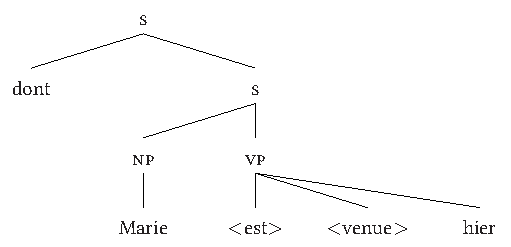
\includegraphics{figures/Ch3Fig1.pdf} % \documentclass[12pt]{article}
\usepackage[latin1]{inputenc}
%\documentclass[twoside,14pt,a4paper]{article}
\usepackage{fullpage}
%\usepackage{times}
\usepackage{latexsym}
\usepackage{ecltree+}
\usepackage{avm}
\usepackage{avm+}
%\usepackage[utf8]{inputenc}
%\usepackage[francais]{babel}

\usepackage{combelow}

\usepackage{xyling}

\begin{document}


\noindent{\textbf{Figure 1 \hspace{1cm} Analyse par reconstruction syntaxique}}
\vspace{1mm}

\Tree[2]{         & \K{\textsc{s}}\B{dl}\B{dr}       & \\
              \K{dont} && \K{\textsc{s}}\B{dl}\B{d}     & \\
               & \K{\textsc{np}}\B{d} & \K{\textsc{vp}}\B{d}\B{dr}\B{drr} & &\\  
       & \K{Marie} & \K{$<$est$>$} & \K{$<$venue$>$} & \K{hier}}


\bigskip



\noindent{\textbf{Figure 2 \hspace{1cm} Analyse en termes de fragment}}
\vspace{1mm}

\Tree[2]{         & \K{\textsc{xp}}\B{dl}\B{dr} &\\  
               \K{dont} && \K{\textsc{xp}}\B{d}\\
       && \K{\textsc{xp}}\B{dl}\B{dr} &\\
      & \K{Marie} && \K{hier}}


\bigskip



\noindent{\textbf{Figure 3 \hspace{1cm} Hi\'erarchie de syntagmes en HPSG, incluant le fragment et le cluster}}
\noindent

\Tree[2] {&& \K[6.2]{\textit{phrase}}\Bkk{6.2,0}{0,0}{dl}\Bkk{6.2,0}{0,0}{drr}		\\
&\K{\textit{non-hd-ph}}\B{dl}\B{dr} &&& \K{\textit{hd-ph}}\B{dl}\B{dr}\B{drrr} \\ 
\K{\textbf{\textit{cluster-ph}}} & &  \K{\textit{coord-ph}} & \K{\textit{hd-only-ph}}\B{d} && \K{\textit{hd-adj-ph}} && \K{\textit{hd-nexus-ph}}\B{dll}\B{dl}\B{d}\B{dr}\\
& & & \K{\textbf{\textit{hd-fragm-ph}}} && \K{\textit{hd-comps}} & \K{\textit{hd-subj}} & \K{\textit{hd-filler}} & \K{\textit{...}}}


%\bigskip
\newpage



\noindent{\textbf{Figure 4 \hspace{1cm} Repr\'esentation simplifi\'ee d'un fragment contenant un cluster de deux constituants}}

\regAvmFonts\avmoptions{center}

\newcommand{\AVMXPone}{\begin{Avm}{XP}
        \[\tp{head-fragment-ph}\\ synsem & \@{2} \[head \@{1}\]\\ mrkg & nil \]
        \end{Avm} }
\newcommand{\AVMXPtwo}{\begin{Avm}{XP}
				\[\tp{cluster-ph} \\ synsem & \@{2} \[head \@{1} & \[cluster & \<\@{3}, \@{4} \> \] \] \] 
				\end{Avm}} 
\newcommand{\AVMNPone}{\begin{Avm}{NP}
    \[synsem & \@{3} \]
\end{Avm}}
\newcommand{\AVMNPtwo}{\begin{Avm}{NP}
    \[synsem & \@{4} \] 
    \end{Avm}}       
    

\smallAvmFonts
\begin{figure}[hbcd]
  \begin{center}
     \begin{bundle}{\AVMXPone}\setlength{\GapDepth}{40pt}
       \chunk[\textsc{hd}]{\setlength{\GapWidth}{45pt}
       		\begin{bundle}{\AVMXPtwo}
               \chunk[\textsc{n-hd}]{\setlength{\GapWidth}{70pt}\setlength{\GapDepth}{20pt}
                  \begin{bundle}{\AVMNPone}
                    \chunk{Marie}
                  \end{bundle}}
               \chunk[\textsc{n-hd}]{\setlength{\GapDepth}{20pt}
                  \begin{bundle}{\AVMNPtwo}
                    \chunk{hier}
                  \end{bundle}}
             \end{bundle}}
             
         \end{bundle}
       	      
    
  \end{center}
\end{figure}
\regAvmFonts


\newpage



\noindent{\textbf{Figure 5 \hspace{1cm} Repr\'esentation simplifi\'ee d'un fragment contenant un cluster unaire}}

\regAvmFonts\avmoptions{center}

\newcommand{\AVMXPthree}{\begin{Avm}{XP}
        \[\tp{head-fragment-ph}\\ synsem & \@{2} \[head \@{1}\]\\ mrkg & nil \]
        \end{Avm} }
\newcommand{\AVMXPfour}{\begin{Avm}{XP}
				\[\tp{cluster-ph} \\ synsem & \@{2} \[head \@{1} & \[cluster & \<\@{3}NP \> \] \] \] 
				\end{Avm}} 
\newcommand{\AVMNPthree}{\begin{Avm}{NP}
    \[synsem & \@{3} \]
\end{Avm}}
          

\smallAvmFonts
\begin{figure}[hbcd]
  \begin{center}
     \begin{bundle}{\AVMXPthree}\setlength{\GapDepth}{40pt}
       \chunk[\textsc{hd}]{\setlength{\GapWidth}{45pt}
       		\begin{bundle}{\AVMXPfour}
               \chunk[\textsc{n-hd}]{\setlength{\GapWidth}{70pt}\setlength{\GapDepth}{20pt}
                  \begin{bundle}{\AVMNPthree}
                    \chunk{Marie}
                  \end{bundle}}
               
             \end{bundle}}
             
         \end{bundle}
       	      
    
  \end{center}
\end{figure}
\regAvmFonts


\bigskip



\noindent{\textbf{Figure 6 \hspace{1cm} Relations fonctionnelles possibles dans la RSV}
\vspace{1mm}

\noindent
\Tree{ &&& \K{\textsc{xp}}\B{dll}_{?}\B{drr}^{HD}  &&&\\
          & \K{\textsc{pp}}\B{dl}\B{dr} & && & \K{\textsc{xp}}\B{d} &\\                         
\K{dintre} && \K{care} &&& \K{\textsc{xp}}\B{dl}\B{dr}\\
&&&&      \K{una} && \K{ieri}}

\paragraph{}

\Tree{&&& \K{\textsc{pp}}\B{dll}_{HD}\B{drr}^{?} &&&\\
          & \K{\textsc{pp}}\B{dl}\B{dr} & && & \K{\textsc{xp}}\B{d} &\\                         
\K{dintre} && \K{care} &&& \K{\textsc{xp}}\B{dl}\B{dr}\\
&&&&      \K{una} && \K{ieri}}

\paragraph{}

\Tree{&&& \K{\textsc{xp}}\B{dll}_{N-HD}\B{drr}^{N-HD} &&&\\
       & \K{\textsc{pp}}\B{dl}\B{dr} & && & \K{\textsc{xp}}\B{d} &\\                         
\K{dintre} && \K{care} &&& \K{\textsc{xp}}\B{dl}\B{dr}\\
&&&&      \K{una} && \K{ieri}}


\bigskip



\noindent{\textbf{Figure 7 \hspace{1cm} Le syntagme de type t\^ete-foncteur dans une hi\'erarchie de syntagmes}

\noindent
\Tree[2]{ & \K[5.2]{\textit{phrase}}\Bkk{5.2,0}{0,0}{dl}\Bkk{5.2,0}{0,0}{dr}		\\
\K{\textit{non-hd-ph}}	&			 & \K[5.2]{\textit{hd-ph}}\Bkk{5.2,0}{0,0}{dl}\Bkk{5.2,0}{0,0}{dr}\Bkk{5.2,0}{0,0}{drrrr}  \\
& \K{\textit{hd-only-ph}}\B{d} & &   \K{\textit{hd-adj-ph}}\B{d}\B{dr} &&& \K{\textit{hd-nexus-ph}}\B{dl}\B{dr}\B{drr}\\
& \K{\textit{hd-fragm-ph}} && \K{\textbf{\textit{hd-funct-ph}}} & \K{\textit{...}} & \K{\textit{hd-comps-ph}} && \K{\textit{hd-subj-ph}} & \K{\textit{...}}}


\bigskip



\noindent{\textbf{Figure 8 \hspace{1cm} Arbre avec un syntagme t\^ete-foncteur}}

\regAvmFonts\avmoptions{center}
\newcommand{\AVMXPfive}{\begin{Avm}{XP}
        \[\tp{head-functor-ph}\\ head & \@{1}\\ mrkg & \@{2} marked\]
      									\end{Avm}}
\newcommand{\AVMPPone}{\begin{Avm}{PP}
        \[cat & \[head & \[select & \@{3}\]\\ mrkg & \@{2}\]\]
      									\end{Avm}}
\newcommand{\AVMXPsix}{\begin{Avm}{XP}
  \@{3}\[cat & \[head & \@{1}\\ mrkg & unmarked\]\]
      									\end{Avm}}
\newcommand{\AVMXPsixbis}{\begin{Avm}{XP} 
        							 \end{Avm}}
\newcommand{\AVMNPfirst}{\begin{Avm}{NP} 
        							 \end{Avm}}


\smallAvmFonts
\begin{figure}[hbcd]
  \begin{center}\setlength{\GapWidth}{60pt}\setlength{\GapDepth}{30pt}
     \begin{bundle}{\AVMXPfive}     	  			
     \chunk[\textsc{fct}]{\setlength{\GapWidth}{60pt}\setlength{\GapDepth}{20pt}
         \begin{bundle}{\AVMPPone}
           \chunk{parmi}
           \chunk{lesquelles}
         \end{bundle}}
     
  		\chunk[\textsc{hd}]{\setlength{\GapWidth}{60pt}\setlength{\GapDepth}{15pt}
         \begin{bundle}{\AVMXPsix}
         	\chunk{\setlength{\GapDepth}{15pt}\begin{bundle}{\AVMXPsixbis}
         	 \chunk{\setlength{\GapDepth}{15pt}\begin{bundle}{\AVMNPfirst}
           \chunk{Marie}
           \end{bundle}}
           \end{bundle}}  
         \end{bundle}}
 
     \end{bundle}
         
  \end{center}
\end{figure}
\regAvmFonts


\newpage



\noindent{\textbf{Figure 9 \hspace{1cm} Syntaxe simplifi\'ee des constructions \`a RSV en fran\c{c}ais}}

\Tree{ &&& \K{\textsc{s}}\B{dll}_{HD}\B{drrr}^{ADJ}  &&\\
& \K{\textsc{s}}\B{dl}_{SUBJ}\B{dr}^{HD} & && && \K{\textsc{xp}}\B{dl}_{FCT}\B{drr}^{HD} &\\ 
\K{\textsc{np}}\TRi && \K{\textsc{v}}\B{d} &&& \K{\textsc{pp}}\B{dl}_{HD}\B{dr}^{COMPS} & && \K{\textsc{xp}}\B{d}^{HD} &\\
\K{plusieurs}\Below{personnes} && \K{chantent} && \K{\textsc{p}rep}\B{d} && \K{\textsc{np}}\TRi && \K{\textsc{xp}}\B{d}^{N-HD}\\
&&&& \K{parmi} && \K{lesquelles} && \K{\textsc{np}}\TRi\\
&&&& && & & \K{Marie}}


\bigskip



\noindent{\textbf{Figure 10 \hspace{1cm} Syntaxe simplifi\'ee des constructions \`a RSV en roumain}}

\Tree{ &&& \K{\textsc{s}}\B{dll}_{HD}\B{drrr}^{ADJ}  &&\\
& \K{\textsc{s}}\B{dl}_{HD}\B{dr}^{SUBJ} & && && \K{\textsc{xp}}\B{dl}_{FCT}\B{drr}^{HD} &\\ 
\K{\textsc{v}}\B{d} && \K{\textsc{np}}\TRi &&& \K{\textsc{pp}}\B{dl}_{HD}\B{dr}^{COMPS} & && \K{\textsc{xp}}\B{d}^{HD} &\\
\K{vin} && \K{mai}\Below{multe}\Below{persoane} && \K{\textsc{p}rep}\B{d} && \K{\textsc{np}}\TRi && \K{\textsc{xp}}\B{d}^{N-HD}\\
&&&& \K{printre} && \K{care} && \K{\textsc{np}}\TRi\\
&&&& && & & \K{\c{s}i Maria}}

  
\newpage



\noindent{\textbf{Figure 11 \hspace{1cm} Relation \`a distance entre l'introducteur et l'\'el\'ement distingu\'e: accessibilit\'e de l'\'el\'ement distingu\'e dans le corps de la RSV}}      									      				

\regAvmFonts\avmoptions{center}
\newcommand{\AVMXPseven}{\begin{Avm}{XP}
        \[\tp{head-functor-ph} \\ ss & \[ head & \@{6} noun \\ mrkg & \@{7} \\ rel & \{\@{4}\} \] \] 
        									\end{Avm}}
        									
\newcommand{\AVMPPtwo}{\begin{Avm}{PP}
        \[\tp{head-comps-ph} \\ ss & \[ head & \[select & \@{1}  \] \\ mrkg & \@{7}\\ rel & \{\@{4}\} \] \] 
        							 \end{Avm}}
        							 
\newcommand{\AVMPrepone}{\begin{Avm}{Prep}
  			\[cat & \[head & \[select & \@{1} \[cont & \[anchors & \<\[ind & \@{3}\]\>\]\]\] \\ mrkg & \@{7}\\ val & \[comps & \<\@{2}\>\] \\ arg-st & \<\@{1}, \@{2}\> \] \\
  			  cont & \[ltop & \@{5} \\ rels & \<\[\tp{sum-subpart-rel} \\ label & \@{5} \\ subpart & \@{3} \\ sum & \@{4} \] \> \] \]
      									\end{Avm}}
      									
\newcommand{\AVMNPfour}{\begin{Avm}{NP}
   \[ss &\@{2}\[cat & \[head & noun\]\\ cont & \[ind & \@{4}\] \\ rel & \{\@{4}\}\] \]
        							 \end{Avm}}

\newcommand{\AVMXPeight}{\begin{Avm}{XP}
   \[\tp{head-fragment-ph} \\ ss &\@{1}\[cat & \[head & \@{6} noun\]\\ cont & \[ind & \@{3}\] \]\] 
        							 \end{Avm}}
        							 
\newcommand{\AVMXPeightbis}{\begin{Avm}{XP} 
        							 \end{Avm}}
\newcommand{\AVMNPsecond}{\begin{Avm}{NP} 
        							 \end{Avm}}        							 

\smallAvmFonts
\begin{figure}[hbcd]
  \begin{center}\setlength{\GapWidth}{100pt}\setlength{\GapDepth}{30pt}
     \begin{bundle}{\AVMXPseven}     	  			
   		\chunk[\textsc{fct}]{\setlength{\GapWidth}{140pt}\setlength{\GapDepth}{20pt}
         \begin{bundle}{\AVMPPtwo}
         	 \chunk[\textsc{hd}]{
         	 	\begin{bundle}{\AVMPrepone}
           		\chunk{parmi}
         		 \end{bundle}}
         	  \chunk[\textsc{comps}]{
         	 	 \begin{bundle}{\AVMNPfour}
           	 	\chunk{lesquelles}
         		 \end{bundle}}
         	\end{bundle}}
       \chunk[\textsc{hd}]{\setlength{\GapDepth}{15pt}
         	 	 \begin{bundle}{\AVMXPeight}
           	 	\chunk{\setlength{\GapDepth}{15pt}\begin{bundle}{\AVMXPeightbis}
         	 \chunk{\setlength{\GapDepth}{15pt}\begin{bundle}{\AVMNPsecond}
           \chunk{Marie}
           \end{bundle}}
           \end{bundle}}
         		 \end{bundle}}
      \end{bundle}
         
  \end{center}
\end{figure}
\regAvmFonts


\newpage



\noindent{\textbf{Figure 12 \hspace{1cm} Relation \`a distance entre la RSV et son ant\'ec\'edent: accessibilit\'e de l'ant\'ec\'edent dans la phrase h\^ote}}

\regAvmFonts\avmoptions{center}
\newcommand{\AVMSone}{\begin{Avm}{S}
        \[\tp{head-functor-ph}\] 
       							 \end{Avm}}
        							 
\newcommand{\AVMStwo}{\begin{Avm}{S}
   \[ss & \@{2}\[cont & \[ind & \@{6} \\ rels & \@{9}\] \] \]
        							 \end{Avm}}
        							 
\newcommand{\AVMNPfive}{\begin{Avm}{NP$_i$}
    	 \[cont & \[ind & \@{4}\] \] 
        							 \end{Avm}}

\newcommand{\AVMVone}{\begin{Avm}{V} 
        							 \end{Avm}}
        							         							 
\newcommand{\AVMXPnine}{\begin{Avm}{XP}
        \[ss & \[cat & \[head & \@{1} \[select & \@{2}\[ cont \[ anchors & \<\[ind & \@{4}\]\>\]\]\] \\
         mrkg & \@{10} \] \\
         cont & \[ind & \@{7}\]\\
         c-cont & \[rels & \<\[\tp{sum-subpart-rel}\\ 
         											subpart & \@{7} event\\
         											sum & \@{6} event\]\>\] \\
											rel & \{\@{4}\}\] \]
        									\end{Avm}}
        									        							 
\newcommand{\AVMPPthree}{\begin{Avm}{PP}
  			 \[ss &\[cat & \[head & \[select & \@{3} \] \\
         mrkg & \@{10} \]\\
			cont & \[ltop & \@{5} \\ rels & \<\[\tp{sum-subpart-rel} \\ label & \@{5} \\ subpart & \@{8} \\ sum & \@{4} \] \> \] \\
			rel & \{\@{4}\}\] \]
      									\end{Avm}}
      									
\newcommand{\AVMXPten}{\begin{Avm}{XP}
   			\[ss &\@{3}\[cat \[head & \@{1}\] \\ 
			cont \[ind  \@{7}\\
   								anchors & \<\[ind & \@{8}\]\>\]\\
   				fragment \[source \[ind & \@{6} \\ rels & \@{9}\]\\
   										abstract-cont \@{B}\]\] \]
        							 \end{Avm}}

\newcommand{\AVMXPtenbis}{\begin{Avm}{XP} 
        							 \end{Avm}}
\newcommand{\AVMNPthird}{\begin{Avm}{NP} 
        							 \end{Avm}}

\smallAvmFonts
\begin{figure}[hbcd]
  \begin{center}\setlength{\GapDepth}{25pt}
     \begin{bundle}{\AVMSone}     	  			
   		\chunk[\textsc{hd}]{
         \begin{bundle}{\AVMStwo}
         	 \chunk[\textsc{subj}]{
         	 	\begin{bundle}{\AVMNPfive}
           		\chunk{plusieurs personnes}
         		 \end{bundle}}
    
         	  \chunk[\textsc{hd}]{
         	 	 \begin{bundle}{\AVMVone}
           	 	\chunk{chantent}
         		 \end{bundle}}
         		 \end{bundle}}
         	
     \chunk[\textsc{fct}]{\setlength{\GapWidth}{110pt}\setlength{\GapDepth}{30pt}
       \begin{bundle}{\AVMXPnine}
         	\chunk[\textsc{fct}]{\setlength{\GapWidth}{30pt}
         	 	\begin{bundle}{\AVMPPthree}
           		\chunk{parmi}
           		\chunk{lesquelles$_i$}
         		 \end{bundle}}
          \chunk[\textsc{hd}]{\setlength{\GapWidth}{20pt}\setlength{\GapDepth}{15pt}
         	 	\begin{bundle}{\AVMXPten}
           	 	\chunk{\setlength{\GapDepth}{15pt}\begin{bundle}{\AVMXPtenbis}
         	 \chunk{\setlength{\GapDepth}{15pt}\begin{bundle}{\AVMNPthird}
           \chunk{Marie}
           \end{bundle}}
           \end{bundle}}
         		 \end{bundle}}	 
         	 \end{bundle}}
         	 	
        \end{bundle}
         
  \end{center}
\end{figure}
\regAvmFonts


\newpage



\noindent{\textbf{Figure 13 \hspace{1cm} Arbre avec le compl\'ementeur \textit{dont} dans les relatives ordinaires}}

\regAvmFonts\avmoptions{center}

\newcommand{\AVMNPsix}{\begin{Avm}{NP}
        \[\tp{head-functor-ph}\]
      \end{Avm}}
\newcommand{\AVMNPseven}{\begin{avm} \@1NP$_i$
      \end{avm}}
\newcommand{\AVMSthree}{\begin{Avm}{S}
    \[head & \[select & \@{1} \] \\ mrkg & dont \\ slash & \{ \} \] 
    \end{Avm}}
\newcommand{\AVMCompr}{\begin{Avm}{Compr}
    \[head & \[vform & \@{2}\]\\ mrkg & dont \\ comps & \<\@{3}\>\\ bind & \{\@{4}\} \\ slash & \{\} \]
		\end{Avm}}
\newcommand{\AVMSfour}{\begin{Avm}{S}
\@{3}\[vform & \@{2} tensed \\ subj & \< \>\\ slash & \{\@{4}PP$_i$[\textit{de}] \}\\ mrkg & unmarked \]
\end{Avm}}
\newcommand{\AVMNPeight}{\begin{Avm}{NP}
    \end{Avm}}
\newcommand{\AVMVtwo}{\begin{Avm}{V}
		\[slash & \{\@{4}\}\]
    \end{Avm}}
    
\smallAvmFonts
\begin{figure}[hbcd]

\begin{center}\setlength{\GapWidth}{40pt}\setlength{\GapDepth}{20pt}
     \begin{bundle}{\AVMNPsix}
     
\chunk[\textsc{hd}]{\setlength{\GapDepth}{30pt}
			\begin{bundle}{\AVMNPseven}
               \chunk{l'histoire}
               \end{bundle}
         }

\chunk[\textsc{fct}]{\setlength{\GapWidth}{80pt}\setlength{\GapDepth}{20pt}
         \begin{bundle}{\AVMSthree}
           \chunk[\textsc{hd}]{
             \begin{bundle}{\AVMCompr}
             		\chunk{dont}
               		\end{bundle}
        			 }
             
               \chunk[\textsc{comps}]{
                  \begin{bundle}{\AVMSfour}
                    \chunk[\textsc{subj}]{
                      \begin{bundle}{\AVMNPeight}
                      \chunk{Marie}
               		\end{bundle}
        			 }
                  
               \chunk[\textsc{hd}]{
                  \begin{bundle}{\AVMVtwo}
                    \chunk{parle}
                  \end{bundle}}
             \end{bundle}
           }
         \end{bundle}
       }
     
     \end{bundle}
  \end{center}
\end{figure}
\regAvmFonts


\newpage



\noindent{\textbf{Figure 14 \hspace{1cm} Arbre avec l'introducteur \textit{dont} dans les RSV}}

\regAvmFonts\avmoptions{center}
\newcommand{\AVMSfive}{\begin{Avm}{S}
        \[\tp{head-functor-ph}\] 
       							 \end{Avm}}
        							 
\newcommand{\AVMSsix}{\begin{Avm}{S}
    \[\tp{head-subject-ph} \\ ss & \@{2}\[cont & \[ind & \@{6}\] \] \]
        							 \end{Avm}}
        							 
\newcommand{\AVMNPnine}{\begin{Avm}{NP}
    	 \[ss & \[cont & \[ind & \@{4}\] \] \] 
        							 \end{Avm}}

\newcommand{\AVMVthree}{\begin{Avm}{V} 
        							 \end{Avm}}
        							         							 
\newcommand{\AVMXPeleven}{\begin{Avm}{XP}
        \[\tp{head-functor-ph} \\ ss & \[cat & \[head \@{1} & \[select & \@{2} \] \\ mrkg & dont \] \] \]
        									\end{Avm}}
        									        							 
\newcommand{\AVMYPone}{\begin{Avm}{?P}
  			\[ss & \[cat & \[head & \[select & \[cat \[head \| select \@{7} \| cont \[anchors & \<\[ind & \@{4}\]\> \] \] \\ cont \[anchors & \<\[ind & \@{3}\]\> \] \] \] \\ mrkg & dont\] \\
  			cont & \[ltop & \@{5} \\ rels & \<\[\tp{sum-subpart-rel} \\ label & \@{5} \\ subpart & \@{3} \\ sum & \@{4} \] \> \] \] \]
      									\end{Avm}}
      									
\newcommand{\AVMXPtwelve}{\begin{Avm}{XP}
   \[\tp{head-fragment-phrase}\\ ss & \@{7}\[cat & \[head & \@{1}\] \\ cont & \[ind & \@{3}\]\] \]
        							 \end{Avm}}

\newcommand{\AVMXPtwelvebis}{\begin{Avm}{XP} 
        							 \end{Avm}}
\newcommand{\AVMNPfourth}{\begin{Avm}{NP} 
        							 \end{Avm}}

\smallAvmFonts
\begin{figure}[hbcd]
  \begin{center}\setlength{\GapWidth}{50pt}\setlength{\GapDepth}{25pt}
     \begin{bundle}{\AVMSfive}     	  			
   		\chunk[\textsc{hd}]{\setlength{\GapWidth}{10pt}
         \begin{bundle}{\AVMSsix}
         	 \chunk[\textsc{subj}]{\setlength{\GapDepth}{15pt}
         	 	\begin{bundle}{\AVMNPnine}
           		\chunk{plusieurs personnes}
         		 \end{bundle}}
    
         	  \chunk[\textsc{hd}]{\setlength{\GapDepth}{19pt}
         	 	 \begin{bundle}{\AVMVthree}
           	 	\chunk{chantent}
         		 \end{bundle}}
         		 \end{bundle}}
         	
     \chunk[\textsc{fct}]{\setlength{\GapWidth}{200pt}\setlength{\GapDepth}{80pt}
       \begin{bundle}{\AVMXPeleven}
         	\chunk[\textsc{fct}]{\setlength{\GapWidth}{100pt}\setlength{\GapDepth}{40pt}
         	 	\begin{bundle}{\AVMYPone}
           		\chunk{dont}
         		 \end{bundle}}
          		\chunk[\textsc{hd}]{\setlength{\GapWidth}{130pt}\setlength{\GapDepth}{15pt}
         	 	\begin{bundle}{\AVMXPtwelve}
           	 	\chunk{\setlength{\GapDepth}{15pt}
           	 	\begin{bundle}{\AVMXPtwelvebis}
         	 \chunk{\setlength{\GapDepth}{15pt}
         	 \begin{bundle}{\AVMNPfourth}
           \chunk{Marie}
           \end{bundle}}
           \end{bundle}}
         		 \end{bundle}}	 
         	 \end{bundle}}
         	 	
        \end{bundle}
         
  \end{center}
\end{figure}
\regAvmFonts


\end{document}
%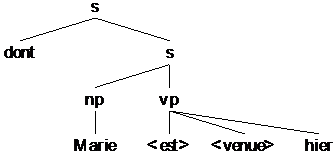
\includegraphics[width=\textwidth]{figures/chap3andconclusion16fevr17-img1.png}
\caption{Analyse par reconstruction syntaxique}
\label{ch3:fig1}
\end{figure} 


\subsection{Reconstruction syntaxique}\label{ch3:sect3.4.1}

Si on adopte une approche elliptique à base de \isi{reconstruction syntaxique}, il y a au moins trois stratégies pour la reconstruction verbale dans les RSV. On peut reconstruire : (i) une forme verbale du même lexème que le verbe de la phrase hôte, cf. \REF{ch3:ex86a} et \REF{ch3:ex87a}, dans les RSV qui contiennent un \isi{cluster} imitant la syntaxe de l’hôte ; (ii) la forme d’un verbe existentiel ou d’un verbe qui paraphrase la relation d’appartenance à un ensemble (p.ex. en roumain les verbes \textit{a fi} ‘être’, \textit{a se afla} ‘se trouver’, \textit{a se găsi} ‘se trouver’ ou en français les verbes \textit{être, figurer,} \textit{faire partie}), cf. \REF{ch3:ex86b} et \REF{ch3:ex87b}, ou bien (iii) la forme d’un verbe de citation (p.ex. en roumain les verbes \textit{a cita} ‘citer’\textit{, a menţiona} ‘mentionner’ ou en français les verbes \textit{citer, mentionner}), cf. \REF{ch3:ex86c} et \REF{ch3:ex87c}.

\ea \label{ch3:ex86}
\ea 
Ion a pictat mai multe tablouri, [\textbf{dintre} \textbf{care} două (\uline{sunt pictate}) la mare]. \label{ch3:ex86a}\\
\glt ‘Ion a peint plusieurs tableaux, dont deux (sont peints) à la mer.’
\ex 
Israelul a omorât peste 700 de palestinieni, [\textbf{dintre care} 200 (\uline{sunt}) copii]. \label{ch3:ex86b}\\
\glt ‘L’état d’Israël a tué plus de 700 Palestiniens, dont 200 (sont) des enfants.’
\ex 
Marin Preda a scris mai multe romane, [\textbf{printre care} (\uline{cităm}) \textit{Moromeţii}]. \label{ch3:ex86c}\\
\glt ‘Marin Preda a écrit plusieurs romans, dont (nous citons) \textit{Moromeţii}.’
\z 
\z

\ea \label{ch3:ex87}
\ea 
Jean a peint beaucoup de tableaux, [\textbf{dont} deux (\uline{ont été peints}) à la mer]. \label{ch3:ex87a}
\ex
Paul a écrit cinq livres, [\textbf{dont} deux (\uline{sont}) sur le même sujet. \label{ch3:ex87b}
\ex 
Zola a écrit beaucoup de romans, [\textbf{dont} (\uline{on peut citer}) \textit{Germinal}]. \label{ch3:ex87c}
\z 
\z

Cependant, ces stratégies ne sont pas disponibles dans tous les contextes. Il n’y a pas un mécanisme général de \isi{reconstruction syntaxique} pouvant s’appliquer à toutes les RSV. Pour chaque exemple, on doit choisir une certaine stratégie. Le type de \isi{reconstruction syntaxique} possible dépend : (i) des propriétés syntaxiques du corps de la RSV, et (ii) du type de sémantique à paraphraser (exemple ou partition). 

Dans une approche à base de \isi{reconstruction syntaxique}, le choix de la forme verbale dépend des contraintes lexicales, comme les propriétés de sous-catégori\-sation, qui ne sont pas corrélées avec les propriétés sémantiques. Si dans une RSV telle qu'en \REF{ch3:ex88a}, la troisième stratégie marche avec les deux introducteurs \textit{dont} et \textit{parmi lesquel(le)s} en français \REF{ch3:ex88b}, la deuxième option obéit à des contraintes particulières, imposées par le comportement syntaxique du verbe reconstruit. Ainsi, en \REF{ch3:ex88c} on peut reconstruire le verbe \textit{figurer} dans une RSV introduite par \textit{parmi lesquel(le)s}, mais pas dans une RSV introduite par \textit{dont}, car le verbe \textit{figurer} peut sous-catégoriser un syntagme prépositionnel introduit par la préposition \textit{parmi}, et non un syntagme prépositionnel introduit par la préposition \textit{de}. En revanche, en \REF{ch3:ex88d} on reconstruit une forme verbale comme l’expression \textit{faire partie}, qui est compatible avec \textit{dont} (car elle sous-catégorise un syntagme prépositionnel en \textit{de}), mais pas avec \textit{parmi lesquel(le)s} (car elle ne sous-catégorise pas un complément marqué par \textit{parmi}).

\ea \label{ch3:ex88}
\ea 
Plusieurs personnes sont venues, [\{\textbf{dont {\textbar} parmi lesquelles}\} Jean]. \label{ch3:ex88a} 
\ex
Plusieurs personnes sont venues, [\{\textbf{dont {\textbar} parmi lesquelles}\} \uline{on peut citer} Jean]. \label{ch3:ex88b}
\ex 
Plusieurs personnes sont venues, [\{*\textbf{dont {\textbar} parmi lesquelles}\} \uline{figure} Jean]. \label{ch3:ex88c}
\ex 
Plusieurs personnes sont venues, [\{\textbf{dont {\textbar} *parmi lesquelles}\} Jean \uline{fait partie}]. \label{ch3:ex88d}
\z 
\z

Dans certains cas, aucune des trois stratégies mentionnées ci-dessus n’est disponible dans les deux langues, car il y a trop de contraintes sur la sous-catégorisa\-tion du verbe reconstruit. Cela arrive surtout dans les RSV qui contiennent un \isi{cluster} de syntagmes. Ainsi en roumain, l’introducteur \textit{printre} \textit{care} n’est compatible avec aucune stratégie de reconstruction verbale en \REF{ch3:ex89}, qu’il s’agisse d’un même lexème verbal que dans la phrase hôte \REF{ch3:ex89b}, d’un verbe existentiel \REF{ch3:ex89c} ou bien d’un verbe de citation \REF{ch3:ex89d}. De même, dans l’exemple \REF{ch3:ex90}, où on a un cluster de constituants (\textit{între 50 şi 60\%} ‘entre 50 et 60\%’ et \textit{vara} ‘l’été’) et l’introducteur \textit{dintre care}, on a du mal à trouver un verbe qui puisse être reconstruit dans une des deux positions possibles, {\cad} avant le premier constituant du \isi{cluster} ou bien entre les deux syntagmes du \isi{cluster}.  

\ea \label{ch3:ex89}
\ea 
\gll La  petrecere,  mai  toţi  au  vorbit  cu  câte  cineva,  [\textbf{printre} \textbf{care} şi  Dan  cu  Ioana]. \label{ch3:ex89a}\\
à  fête  plus  tous  ont  parlé  avec  \textsc{distr}  quelqu’un  parmi  lesquels aussi  Dan  avec  Ioana \\
\glt ‘A la fête, presque tous ont parlé avec quelqu’un, dont Dan avec Ioana.’
\ex 
\gll *La  petrecere,  mai  toţi  au  vorbit  cu  câte  cineva,  [\textbf{printre} \textbf{care} şi  Dan  \ulg{a}{12}  vorbit  cu  Ioana]. \label{ch3:ex89b}\\
à  fête  plus  tous  ont  parlé  avec  \textsc{distr}  quelqu’un  parmi  lesquels aussi  Dan  a  parlé  avec  Ioana \\
\glt ‘A la fête, presque tous ont parlé avec quelqu’un, dont Dan avec Ioana.’
\ex 
\gll *La  petrecere,  mai  toţi  au  vorbit  cu  câte  cineva,  [\textbf{printre} \textbf{care} şi  Dan  \uline{e}  cu  Ioana]. \label{ch3:ex89c}\\
à  fête  plus  tous  ont  parlé  avec  \textsc{distr}  quelqu’un  parmi  lesquels aussi  Dan  est  avec  Ioana \\
\glt ‘A la fête, presque tous ont parlé avec quelqu’un, dont Dan avec Ioana.’
\ex 
\gll *La  petrecere,  mai  toţi  au  vorbit  cu  câte  cineva,  [\textbf{printre} \textbf{care} \uline{menţionăm}  şi  Dan  cu  Ioana]. \label{ch3:ex89d}\\
à  fête  plus  tous  ont  parlé  avec  \textsc{distr}  quelqu’un  parmi  lesquels mentionner.\textsc{prs.1pl}  aussi  Dan  avec  Ioana \\
\glt ‘A la fête, presque tous ont parlé avec quelqu’un, dont Dan avec Ioana.’
\z 
\z

\ea \label{ch3:ex90} 
\gll Media  precipitaţiilor  anuale  este  de  circa  1~000  mm,  [\textbf{dintre} \textbf{care}  (??)  între  50  şi  60\%  (??)  vara].\\
moyenne.\textsc{def}  précipitations.\textsc{gen}  annuelles  est  de  environ  1~000  mm  parmi lesquels  (??)  entre  50  et  60\%  (??)  été.\textsc{def} \\
\glt ‘La moyenne des précipitations annuelles est d’environ 1~000 mm, dont entre 50\% et 60\% l’été.’ 
\z

L’impossibilité de reconstruire un verbe dans les RSV contenant un cluster se manifeste en français aussi, comme illustré en \REF{ch3:ex91} pour l’introducteur \textit{dont}. On voit bien qu’aucune des trois stratégies de reconstruction verbale ne fonctionne en (\ref{ch3:ex91b}--\ref{ch3:ex91d}).

\ea \label{ch3:ex91}
\ea 
Plusieurs ont eu un cadeau, [\textbf{dont} Marie un livre]. \label{ch3:ex91a} 
\ex
*Plusieurs ont eu un cadeau, [\textbf{dont} Marie \uline{a eu} un livre]. \label{ch3:ex91b}
\ex 
*Plusieurs ont eu un cadeau, [\textbf{dont} Marie \uline{est} un livre]. \label{ch3:ex91c}
\ex 
*Plusieurs ont eu un cadeau, [\textbf{dont} \uline{on cite} Marie un livre]. \label{ch3:ex91d}
\z 
\z 

Pour sauver la possibilité de \isi{reconstruction syntaxique} dans les clusters, on pourrait faire appel à une reconstruction plus complexe qui combine une des trois stratégies avec une phrase relative interne. Bien qu’elle marche pour certains exemples, cf. \REF{ch3:ex92c}, cette nouvelle possibilité n’est pas une solution générale pour les deux interprétations disponibles dans les RSV (comparer \REF{ch3:ex92c} et \REF{ch3:ex93c}) et, en plus, elle ne rend pas compte des contraintes pesant sur les syntagmes du cluster dans une RSV, qui doivent être toujours des constituants de même niveau dans la phrase hôte \REF{ch3:ex94}.

\ea \label{ch3:ex92}
\ea 
J’ai vendu 16 jeux, [\textbf{dont} certains à mes amis]. \label{ch3:ex92a} 
\ex
*J’ai vendu 16 jeux, [\textbf{dont} \uline{j’ai vendu} certains à mes amis]. \label{ch3:ex92b}
\ex 
J’ai vendu 16 jeux, [\textbf{dont} \uline{on peut citer} certains \uline{que j’ai vendu} à mes amis]. \label{ch3:ex92c}
\z 
\z 

\ea \label{ch3:ex93} 
\ea 
J’ai parlé à plusieurs personnes hier, [\textbf{dont} à Marie de linguistique]. \label{ch3:ex93a} 
\ex
*J’ai parlé à plusieurs personnes hier, [\textbf{dont} \uline{j’ai parlé} à Marie de linguistique]. \label{ch3:ex93b}
\ex 
*J’ai parlé à plusieurs personnes hier, [\textbf{dont} \uline{on peut citer que j’ai parlé} à Marie de linguistique]. \label{ch3:ex93c}
\z 
\z

\ea \label{ch3:ex94} 
??/*Mes amis croient que la vie existe sur d’autres planètes, [\textbf{dont} Marie sur Mars].   
\z

Un argument supplémentaire contre la reconstruction verbale dans les RSV est dû aux propriétés de l’introducteur \textit{dont} et des syntagmes nominaux sans tête lexicalisée, qui sont d’ailleurs très fréquents avec les RSV \REF{ch3:ex95a}. Les syntagmes nominaux sans tête qui fonctionnent comme des compléments directs d’un verbe déclenchent la réalisation de \is{affixe/clitique pronominal}l’affixe pronominal \textit{en} sur le verbe \REF{ch3:ex95b}. Cependant, les RSV avec \textit{dont} ne permettent aucune reconstruction, qu’il s’agisse ou non de l’affixe \textit{en} (\ref{ch3:ex95c}--\ref{ch3:ex95d}), car de toute façon \textit{dont} est incompatible avec la réalisation de l’affixe \textit{en} sur le verbe.

\ea \label{ch3:ex95}
\ea 
Il a offert \uline{trois livres}, [\textbf{dont} \uline{deux} à son frère]. \label{ch3:ex95a}
\ex
Il *(\uline{en}) a offert \uline{deux} à son frère. \label{ch3:ex95b}
\ex 
*... \textbf{dont} il a offert \uline{deux} à son frère. \label{ch3:ex95c}
\ex 
*... \textbf{dont} il \uline{en} a offert \uline{deux} à son frère. \label{ch3:ex95d}
\z 
\z

En même temps, si on envisage une \isi{reconstruction syntaxique} dans les RSV, on ne peut pas expliquer pourquoi le \isi{marquage casuel} ou \is{marquage prépositionnel}prépositionnel en roumain est interdit avec les RSV introduites par \textit{dintre care} \REF{ch3:ex96}, alors qu’il est possible avec les RSV introduites par \{\textit{printre / între}\} \textit{care} \REF{ch3:ex97}, étant donné que les deux prépositions ont le même comportement syntaxique en dehors des RSV.

\ea \label{ch3:ex96}
\ea 
\gll Ion  a  oferit  flori  mai  mult\uline{or}  persoane,  [\textbf{dintre}  \textbf{care} \{majoritatea  {\textbar}  *majorităţ\uline{ii}\}  fete]. \label{ch3:ex96a}\\
Ion  a  offert  fleurs  plus  beaucoup.\textsc{adj.dat}  personnes  parmi  lesquelles \{majorité.\textsc{def} {\textbar}  majorité.\textsc{dat}\}  filles \\
\glt ‘Ion a offert des fleurs à plusieurs personnes, dont la plupart des filles.’
\ex 
\gll Dragoş  lucrează  \uline{cu}  şapte  medici,  [\textbf{dintre} \textbf{care}  (*\uline{cu})  doi  israelieni]. \label{ch3:ex96b}\\
Dragoş  travaille  avec  sept  médecins  parmi  lesquels  (avec) deux  Israéliens \\
\glt ‘Dragoş travaille avec sept médecins, dont deux Israéliens.’
\z 
\z

\ea \label{ch3:ex97}
\ea 
\gll Ion  a  oferit  flori  mai  mult\uline{or} fete,  [\textbf{printre} \textbf{care}  şi   \{Maria {\textbar} Mari\uline{ei}\}]. \label{ch3:ex97a}\\
Ion  a  offert  fleurs  plus  beaucoup.\textsc{adj.dat}  filles  parmi  lesquelles  aussi \{Maria {\textbar} Maria.\textsc{dat}\} \\
\glt ‘Ion a offert des fleurs à plusieurs filles, parmi lesquelles Maria.’ 
\ex 
\gll Ion  a  vorbit  cu  mai  multe  fete,  [\textbf{printre} \textbf{care}  şi  (cu) Maria]. \label{ch3:ex97b}\\
Ion  a  parlé  avec  plus  beaucoup.\textsc{adj}  filles  parmi  lesquelles  aussi  (avec) Maria \\
\glt ‘Ion a parlé avec plusieurs filles, parmi lesquelles Maria.’
\z 
\z

Dans d’autres cas, le choix de la stratégie est influencé par le type de sémantique observé dans la RSV. Ainsi, la troisième stratégie, qui utilise un verbe de citation comme moyen de reconstruction, est appropriée pour les RSV à \isi{interprétation exemplifiante} (cf. l’exemple \REF{ch3:ex98a} en roumain et \REF{ch3:ex99a} en français), mais inacceptable dans le cas des RSV avec une \isi{interprétation partitionnante} (cf. l’exemple \REF{ch3:ex98b} en roumain et \REF{ch3:ex99b} en français).

\ea \label{ch3:ex98}
\ea 
Marin Preda a scris mai multe romane, [\textbf{printre care} (\uline{menţionăm}) \textit{Moromeţii}]. \label{ch3:ex98a}\\
\glt ‘Marin Preda a écrit plusieurs romans, dont (nous mentionnons) \textit{Moromeţii}.’
\ex 
Săptămâna aceasta, Ion a cheltuit 1~000 de euro, [\textbf{dintre} \textbf{care} (\#\uline{menţionăm}) 800 numai ieri]. \label{ch3:ex98b}\\
\glt ‘Cette semaine, Ion a dépensé 1~000 euros, dont (nous mentionnons) 800 seulement hier.’  
\z 
\z 

\ea \label{ch3:ex99} 
\ea 
Zola a écrit beaucoup de romans, [\textbf{dont} (\uline{on peut citer}) \textit{Germinal}]. \label{ch3:ex99a} 
\ex
Je vends 16 jeux, [\textbf{dont} (\#\uline{on peut citer}) la plupart encore dans leur boîte]. \label{ch3:ex99b}
\z 
\z

De plus, la position du verbe reconstruit change en fonction de la stratégie utilisée : s’il s’agit d’un verbe de citation, il précède nécessairement le corps de la RSV comme en \REF{ch3:ex100b} et \REF{ch3:ex101b}, alors qu’avec les autres stratégies, le verbe suit le premier syntagme du corps, cf. \REF{ch3:ex100a} et \REF{ch3:ex101a}.

\ea \label{ch3:ex100}
\ea ... patru persoane, [\textbf{dintre care} una (\uline{este}) cetăţean american]. \label{ch3:ex100a}\\
\glt ‘... quatre personnes, dont l’une (est) citoyen américain.’

\ex ... patru persoane, [\textbf{printre care} (\uline{amintim}) un cetăţean american]. \label{ch3:ex100b}\\
\glt ‘... quatre personnes, parmi lesquelles (on mentionne) un citoyen américain.’ 
\z 
\z


\ea \label{ch3:ex101}
\ea
... quatre journalistes, [\textbf{dont} l’un (\uline{est}) citoyen américain]. \label{ch3:ex101a}
\ex
... quatre journalistes, [\textbf{dont} (\uline{on peut citer})\textbf{} un citoyen américain]. \label{ch3:ex101b} 
\z 
\z 

On observe ainsi qu’il n’y a pas de mécanisme général de reconstruction qui s’applique à toutes les RSV. Si ce mécanisme est disponible, des contraintes lexicales, syntaxiques ou sémantiques doivent être prises en compte pour chaque cas. Comme il s’agit d’un mécanisme ad-hoc et superflu, la \isi{reconstruction syntaxique} doit être abandonnée.  


\subsection{Différences sémantiques}\label{ch3:sect3.4.2}

Si on considère que les RSV sont des phrases relatives elliptiques dérivées à partir des phrases relatives verbales, on s’attend à ce que leur contribution sémantique soit la même. Or, on observe que les RSV n’ont pas les mêmes propriétés sémantiques que les phrases relatives ordinaires.


\subsubsection{Contenu (non-)parenthétique}\label{ch3:sect3.4.2.1}

Dans la section~\ref{ch3:sect3.3.1}, on a vu que les phrases relatives non restrictives se comportent sémantiquement comme des phrases indépendantes qui contiennent une proforme \citep{Arnold2004}, se prêtant à une analyse en termes \is{implicature conventionnelle}d’implicatures con\-ventionnelles. Par conséquent, leur contribution sémantique est largement indépendante par rapport à celle de la phrase hôte. En revanche, le contenu des RSV n’est pas \is{contenu parenthétique}parenthétique, {\cad} il fait partie du contenu asserté de la phrase hôte, comme le montre le contraste en \REF{ch3:ex102}. Si l’exemple \REF{ch3:ex102a}, qui contient une phrase relative complète, est cohérent, la séquence des énoncés en \REF{ch3:ex102b} contenant une RSV est contradictoire, car on assume à la fois la présence et l’absence des oreilles apparentes chez les baleines. 

\ea \label{ch3:ex102}
\ea 
Non, tu te trompes! Bien que la plupart des mammifères, [\textbf{dont} les baleines font effectivement partie], aient des oreilles apparentes, les baleines, elles, n’en ont pas. \label{ch3:ex102a} 
\ex
\#Non, tu te trompes ! Bien que la plupart des mammifères, [\textbf{dont} les baleines], aient des oreilles apparentes, les baleines, elles, n’en ont pas. \label{ch3:ex102b} 
\z 
\z 

Un des corrélats empiriques de cette différence sémantique observée entre les RSV et les phrases relatives non restrictives est le fait que les \is{prédicat d'attitude propositionnelle}verbes d’attitude propositionnelle n’ont pas de portée sur le contenu d’une phrase relative non restrictive, cf. \REF{ch3:ex103}, alors que cela n’est pas le cas dans les RSV, {\cad} une RSV est interprétée sous la portée d’un tel verbe (cf. la discussion dans la section~\ref{ch3:sect3.3.1} et l’exemple \REF{ch3:ex104} ci-dessous). 

\ea \label{ch3:ex103}
\ea 
Paul crede că anumite plante, [\textbf{printre care} amintim şi sunătoarea], vindecă ulcerul. \\
\glt ‘Paul croit que certaines plantes, parmi lesquelles nous mentionnons la verveine, soignent les ulcères.’ \\
\ex ${\nRightarrow}$ Paul crede că sunătoarea vindecă ulcerul. \\
\glt ‘Paul croit que la verveine soigne les ulcères.’\\
\ex ${\Rightarrow}$ Sunătoarea vindecă ulcerul.\\
\glt ‘La verveine soigne les ulcères.’
\z 
\z 

\ea \label{ch3:ex104} 
\ea 
Paul crede că anumite plante, [\textbf{printre care} şi sunătoarea], vindecă ulcerul. \\
\glt ‘Paul croit que certaines plantes, dont la verveine, soignent les ulcères.’\\
\ex ${\Rightarrow}$ Paul crede că sunătoarea vindecă ulcerul.\\
\glt ‘Paul croit que la verveine soigne les ulcères.’\\
\ex ${\nRightarrow}$ Sunătoarea vindecă ulcerul.\\
\glt ‘La verveine soigne les ulcères.’
\z 
\z

Contrairement à sa contrepartie verbale, le contenu de la RSV fait nécessairement partie du contenu de la phrase hôte ; par conséquent, une relative verbale  \REF{ch3:ex105} ne permet pas de faire la même inférence logique qu’une RSV \REF{ch3:ex106}. 

\ea \label{ch3:ex105}
\ea 
Certains de mes amis, [\textbf{dont} Marie \{est {\textbar} était\} la plus drôle], sont venus à la fête.
\ex 
${\nRightarrow}$ Marie est venue à la fête.
\z 
\z 

\ea \label{ch3:ex106}
\ea 
Certains de mes amis, [\textbf{dont} Marie], sont venus à la fête.
\ex
${\Rightarrow}$ Marie est venue à la fête.
\z 
\z

Les phrases relatives non restrictives peuvent localement faire un commentaire sur la phrase hôte, alors que les RSV ne le peuvent pas. C’est pour cela que la séquence \textit{Il est donc étrange que Balzac en particulier soit autant boudé des enfants} est une continuation appropriée pour une phrase relative non restrictive \REF{ch3:ex107a}, mais non pour une RSV \REF{ch3:ex107b}.

\ea \label{ch3:ex107}
\ea 
Les grands auteurs du XIXe, [\textbf{dont} Balzac est le plus célèbre], sont beaucoup lus par les enfants. Il est donc étrange que Balzac en particulier soit autant boudé des enfants. \label{ch3:ex107a} 
\ex
Les grands auteurs du XIXe, [\textbf{dont} Balzac], sont beaucoup lus par les enfants. \#Il est donc étrange que Balzac en particulier soit autant boudé des enfants. \label{ch3:ex107b}
\z 
\z

A la lumière de ces différences, on ne peut pas non plus assimiler les RSV aux phrases relatives restrictives, car les RSV ne restreignent pas la dénotation de l’antécédent.


\subsubsection{Rôle de l’introducteur}\label{ch3:sect3.4.2.2}

Un autre problème soulevé par une approche elliptique en termes de \isi{reconstruction syntaxique} est le fait qu’elle prédit la bonne formation de certaines RSV, qui en réalité sont inacceptables pour des raisons sémantiques. Cette approche considère que la sémantique partitive des RSV dérive du prédicat verbal élidé plutôt que de l’introducteur ; or, cette hypothèse ne rend pas compte des contraintes observées avec certains syntagmes prépositionnels dans les RSV.

En roumain, le corps d’une RSV introduite par \textit{dintre care} ne peut pas contenir de syntagme nominal spécifique (référentiel), par exemple un nom propre \REF{ch3:ex108a}. Cependant, on peut facilement reconstruire une forme verbale dans le même contexte et obtenir une phrase relative bien formée \REF{ch3:ex108b}. On observe donc que \is{interprétation exemplifiante}l’interprétation exemplifiante est exclue dans les RSV introduites par \textit{dintre care}, mais disponible avec une forme verbale. 

\ea \label{ch3:ex108}
\ea 
\gll *Au  venit  mai  multe  persoane,  [\textbf{dintre} \textbf{care}  Maria]. \label{ch3:ex108a}\\
\textsc{aux.3pl}  venu  plus  beaucoup.\textsc{adj}  personnes  parmi  lesquelles  Maria \\
\glt ‘Plusieurs personnes sont venues, dont Maria.’
\ex 
\gll Au  venit  mai  multe  persoane,  [\textbf{dintre} \textbf{care}  o amintim  pe  Maria]. \label{ch3:ex108b}\\
\textsc{aux.3pl}  venu  plus  beaucoup.\textsc{adj}  personnes  parmi  lesquelles  \textsc{acc.3sg.f} 
mentionner.\textsc{prs.1pl} \textsc{dom}  Maria \\
\glt ‘Plusieurs personnes sont venues, dont on mentionne Maria.’
\z 
\z 

En français, la différence observée entre la RSV introduite par \textit{dont} en \REF{ch3:ex109a}\footnote{Cet exemple est parfaitement acceptable dans le registre informel.} et la RSV introduite par \textit{parmi lesquelles} en \REF{ch3:ex109b} est inattendue dans une approche à base de \isi{reconstruction syntaxique}, car le prédicat gérant la relation entre la RSV et l’antécédent est supposé être la tête verbale qui manque dans la phrase relative et non l’introducteur. En revanche, dans une \isi{approche non structurale} des RSV, rien n’empêche de considérer que l’introducteur possède des propriétés de sélection en ce qui concerne la constituance du corps de la RSV (p.ex. dans une RSV introduite par \textit{parmi lesquel(le)s}, le corps doit contenir au moins un syntagme nominal). 

\ea \label{ch3:ex109}
\ea 
J’ai parlé à plusieurs personnes, [\textbf{dont} à Marie de linguistique]. \label{ch3:ex109a} 
\ex
*J’ai parlé à plusieurs personnes, [\textbf{parmi lesquelles} à Marie de linguistique]. \label{ch3:ex109b}
\z 
\z


\subsubsection{Sémantique partitive stricte}\label{ch3:sect3.4.2.3}

Le type de relations explicitées par les RSV est beaucoup plus contraint par rapport aux relations qu’on peut avoir quand on emploie une phrase relative partitive ordinaire. 

On a vu que les relations \is{méronymie}méronymiques sont exclues dans les RSV (cf. les exemples \REF{ch3:ex60b} et \REF{ch3:ex61b} de la section~\ref{ch3:sect3.3.2.1}), mais elles sont possibles avec une phrase relative partitive verbale, comme le montre le contraste en \REF{ch3:ex110}.

\ea \label{ch3:ex110}
\ea 
*Paul adore les Suédoises, [\textbf{dont} leurs cheveux]. 
\ex
Les fenêtres de ce château, [\textbf{dont} la peinture est écaillée], doivent être remplacées.
\z 
\z

On a vu également que l’élément distingué dans le corps de la RSV doit être une sous-partie de l’ensemble dénoté par l’antécédent (cf. section~\ref{ch3:sect3.3.2.1}). Bien que le \is{pied-piping}\textit{pied-piping} soit, en principe, possible dans une RSV, uniquement les relations directes ensemble/sous-partie sont autorisées \REF{ch3:ex111a}, alors que les phrases relatives partitives ordinaires n’obéissent pas à une contrainte aussi stricte \REF{ch3:ex111b}.   

\ea \label{ch3:ex111}
\ea 
*J’ai reçu deux pétitions, [\textbf{parmi} les signataires \textbf{desquelles} Jean]. \label{ch3:ex111a} 
\ex
J’ai reçu deux pétitions, [\textbf{parmi} les signataires \textbf{desquelles} figure Jean]. \label{ch3:ex111b} 
\z
\z

Pour conclure, à part le fait que la \isi{reconstruction syntaxique} ne peut pas s’appliquer de façon uniforme à toutes les RSV, on observe que les propriétés sémantiques ne sont pas les mêmes dans les RSV et dans les relatives non restrictives verbales. Par conséquent, \is{approche structurale}l’approche structurale en termes d’ellipse syntaxique ne peut pas rendre compte des propriétés syntaxiques et sémantiques des RSV. 


\section{Une approche constructionnelle des RSV en termes d’ajouts fragmentaires}\label{ch3:sect3.5}
 
On propose ici une \isi{approche non structurale}, qui rend compte et de la forme et du contenu des RSV sans postuler de structure syntaxique «~invisible~». Cette approche alternative reprend et enrichit l’analyse proposée par \citet{BilbiieEtAl2009}. 

Les principales idées pour comprendre l’analyse qu’on propose sont les suivantes : Le corps de la RSV est la tête de la construction. L’introducteur a des propriétés de sélection syntaxique et sémantique vis-à-vis de la tête. L’introducteur a également une contribution sémantique importante et marque la construction. La RSV est un ajout fragmentaire.
 
Dans cette section, je présente tout d’abord la notion sémantique de \is{fragment}\textit{fragment} et je montre comment elle permet la \isi{reconstruction sémantique} d’un contenu propositionnel, à partir de la phrase hôte. Dans un deuxième temps, je présente la notion syntaxique de \is{cluster}\textit{cluster}, qui permet de dériver toute séquence de syntagmes sans tête verbale qui peut constituer le corps de la RSV. Les deux notions ont déjà été introduites dans le chapitre~\ref{ch2} dédié aux coordinations à gapping ; elles seront ici appliquées aux subordonnées RSV. Dans un troisième temps, je m’intéresse aux relations fonctionnelles dans la RSV, en particulier à la relation syntaxique qui s’établit entre le corps et l’introducteur, pour décider de la tête de la RSV. Ensuite, je montre comment les \isi{contraintes de localité} permettent, d’une part, l’accès à l’élément distingué dans le corps de la RSV et, d’autre part, l’accès à l’antécédent dans la phrase hôte. Enfin, je présente l’analyse de la RSV dans son ensemble avec ses deux sous-types, en fonction des deux types d’introducteurs employés : un syntagme prépositionnel contenant une forme \textit{qu-} ou bien l’introducteur \textit{dont}. Je donne les entrées lexicales pour chaque introducteur, ainsi que les contraintes qui définissent les deux sous-types de RSV. La section finit par une présentation des deux \textit{dont} en français : le \textit{dont} des RSV et le complémenteur \textit{dont} dans les relatives verbales. 


\subsection{Théorie des fragments}\label{ch3:sect3.5.1}
 
Toutes les différences enregistrées entre les RSV et leurs contreparties verbales s’expliquent par le fait que les RSV sont des ajouts fragmentaires. Une analyse simplifiée de la structure syntaxique d’une RSV est donnée en \figref{ch3:fig2}.

\begin{figure}
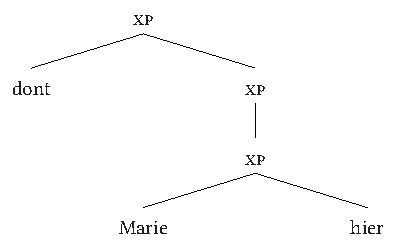
\includegraphics{figures/Ch3Fig2.pdf} % \documentclass[12pt]{article}
\usepackage[latin1]{inputenc}
%\documentclass[twoside,14pt,a4paper]{article}
\usepackage{fullpage}
%\usepackage{times}
\usepackage{latexsym}
\usepackage{ecltree+}
\usepackage{avm}
\usepackage{avm+}
%\usepackage[utf8]{inputenc}
%\usepackage[francais]{babel}

\usepackage{combelow}

\usepackage{xyling}

\begin{document}


\noindent{\textbf{Figure 1 \hspace{1cm} Analyse par reconstruction syntaxique}}
\vspace{1mm}

\Tree[2]{         & \K{\textsc{s}}\B{dl}\B{dr}       & \\
              \K{dont} && \K{\textsc{s}}\B{dl}\B{d}     & \\
               & \K{\textsc{np}}\B{d} & \K{\textsc{vp}}\B{d}\B{dr}\B{drr} & &\\  
       & \K{Marie} & \K{$<$est$>$} & \K{$<$venue$>$} & \K{hier}}


\bigskip



\noindent{\textbf{Figure 2 \hspace{1cm} Analyse en termes de fragment}}
\vspace{1mm}

\Tree[2]{         & \K{\textsc{xp}}\B{dl}\B{dr} &\\  
               \K{dont} && \K{\textsc{xp}}\B{d}\\
       && \K{\textsc{xp}}\B{dl}\B{dr} &\\
      & \K{Marie} && \K{hier}}


\bigskip



\noindent{\textbf{Figure 3 \hspace{1cm} Hi\'erarchie de syntagmes en HPSG, incluant le fragment et le cluster}}
\noindent

\Tree[2] {&& \K[6.2]{\textit{phrase}}\Bkk{6.2,0}{0,0}{dl}\Bkk{6.2,0}{0,0}{drr}		\\
&\K{\textit{non-hd-ph}}\B{dl}\B{dr} &&& \K{\textit{hd-ph}}\B{dl}\B{dr}\B{drrr} \\ 
\K{\textbf{\textit{cluster-ph}}} & &  \K{\textit{coord-ph}} & \K{\textit{hd-only-ph}}\B{d} && \K{\textit{hd-adj-ph}} && \K{\textit{hd-nexus-ph}}\B{dll}\B{dl}\B{d}\B{dr}\\
& & & \K{\textbf{\textit{hd-fragm-ph}}} && \K{\textit{hd-comps}} & \K{\textit{hd-subj}} & \K{\textit{hd-filler}} & \K{\textit{...}}}


%\bigskip
\newpage



\noindent{\textbf{Figure 4 \hspace{1cm} Repr\'esentation simplifi\'ee d'un fragment contenant un cluster de deux constituants}}

\regAvmFonts\avmoptions{center}

\newcommand{\AVMXPone}{\begin{Avm}{XP}
        \[\tp{head-fragment-ph}\\ synsem & \@{2} \[head \@{1}\]\\ mrkg & nil \]
        \end{Avm} }
\newcommand{\AVMXPtwo}{\begin{Avm}{XP}
				\[\tp{cluster-ph} \\ synsem & \@{2} \[head \@{1} & \[cluster & \<\@{3}, \@{4} \> \] \] \] 
				\end{Avm}} 
\newcommand{\AVMNPone}{\begin{Avm}{NP}
    \[synsem & \@{3} \]
\end{Avm}}
\newcommand{\AVMNPtwo}{\begin{Avm}{NP}
    \[synsem & \@{4} \] 
    \end{Avm}}       
    

\smallAvmFonts
\begin{figure}[hbcd]
  \begin{center}
     \begin{bundle}{\AVMXPone}\setlength{\GapDepth}{40pt}
       \chunk[\textsc{hd}]{\setlength{\GapWidth}{45pt}
       		\begin{bundle}{\AVMXPtwo}
               \chunk[\textsc{n-hd}]{\setlength{\GapWidth}{70pt}\setlength{\GapDepth}{20pt}
                  \begin{bundle}{\AVMNPone}
                    \chunk{Marie}
                  \end{bundle}}
               \chunk[\textsc{n-hd}]{\setlength{\GapDepth}{20pt}
                  \begin{bundle}{\AVMNPtwo}
                    \chunk{hier}
                  \end{bundle}}
             \end{bundle}}
             
         \end{bundle}
       	      
    
  \end{center}
\end{figure}
\regAvmFonts


\newpage



\noindent{\textbf{Figure 5 \hspace{1cm} Repr\'esentation simplifi\'ee d'un fragment contenant un cluster unaire}}

\regAvmFonts\avmoptions{center}

\newcommand{\AVMXPthree}{\begin{Avm}{XP}
        \[\tp{head-fragment-ph}\\ synsem & \@{2} \[head \@{1}\]\\ mrkg & nil \]
        \end{Avm} }
\newcommand{\AVMXPfour}{\begin{Avm}{XP}
				\[\tp{cluster-ph} \\ synsem & \@{2} \[head \@{1} & \[cluster & \<\@{3}NP \> \] \] \] 
				\end{Avm}} 
\newcommand{\AVMNPthree}{\begin{Avm}{NP}
    \[synsem & \@{3} \]
\end{Avm}}
          

\smallAvmFonts
\begin{figure}[hbcd]
  \begin{center}
     \begin{bundle}{\AVMXPthree}\setlength{\GapDepth}{40pt}
       \chunk[\textsc{hd}]{\setlength{\GapWidth}{45pt}
       		\begin{bundle}{\AVMXPfour}
               \chunk[\textsc{n-hd}]{\setlength{\GapWidth}{70pt}\setlength{\GapDepth}{20pt}
                  \begin{bundle}{\AVMNPthree}
                    \chunk{Marie}
                  \end{bundle}}
               
             \end{bundle}}
             
         \end{bundle}
       	      
    
  \end{center}
\end{figure}
\regAvmFonts


\bigskip



\noindent{\textbf{Figure 6 \hspace{1cm} Relations fonctionnelles possibles dans la RSV}
\vspace{1mm}

\noindent
\Tree{ &&& \K{\textsc{xp}}\B{dll}_{?}\B{drr}^{HD}  &&&\\
          & \K{\textsc{pp}}\B{dl}\B{dr} & && & \K{\textsc{xp}}\B{d} &\\                         
\K{dintre} && \K{care} &&& \K{\textsc{xp}}\B{dl}\B{dr}\\
&&&&      \K{una} && \K{ieri}}

\paragraph{}

\Tree{&&& \K{\textsc{pp}}\B{dll}_{HD}\B{drr}^{?} &&&\\
          & \K{\textsc{pp}}\B{dl}\B{dr} & && & \K{\textsc{xp}}\B{d} &\\                         
\K{dintre} && \K{care} &&& \K{\textsc{xp}}\B{dl}\B{dr}\\
&&&&      \K{una} && \K{ieri}}

\paragraph{}

\Tree{&&& \K{\textsc{xp}}\B{dll}_{N-HD}\B{drr}^{N-HD} &&&\\
       & \K{\textsc{pp}}\B{dl}\B{dr} & && & \K{\textsc{xp}}\B{d} &\\                         
\K{dintre} && \K{care} &&& \K{\textsc{xp}}\B{dl}\B{dr}\\
&&&&      \K{una} && \K{ieri}}


\bigskip



\noindent{\textbf{Figure 7 \hspace{1cm} Le syntagme de type t\^ete-foncteur dans une hi\'erarchie de syntagmes}

\noindent
\Tree[2]{ & \K[5.2]{\textit{phrase}}\Bkk{5.2,0}{0,0}{dl}\Bkk{5.2,0}{0,0}{dr}		\\
\K{\textit{non-hd-ph}}	&			 & \K[5.2]{\textit{hd-ph}}\Bkk{5.2,0}{0,0}{dl}\Bkk{5.2,0}{0,0}{dr}\Bkk{5.2,0}{0,0}{drrrr}  \\
& \K{\textit{hd-only-ph}}\B{d} & &   \K{\textit{hd-adj-ph}}\B{d}\B{dr} &&& \K{\textit{hd-nexus-ph}}\B{dl}\B{dr}\B{drr}\\
& \K{\textit{hd-fragm-ph}} && \K{\textbf{\textit{hd-funct-ph}}} & \K{\textit{...}} & \K{\textit{hd-comps-ph}} && \K{\textit{hd-subj-ph}} & \K{\textit{...}}}


\bigskip



\noindent{\textbf{Figure 8 \hspace{1cm} Arbre avec un syntagme t\^ete-foncteur}}

\regAvmFonts\avmoptions{center}
\newcommand{\AVMXPfive}{\begin{Avm}{XP}
        \[\tp{head-functor-ph}\\ head & \@{1}\\ mrkg & \@{2} marked\]
      									\end{Avm}}
\newcommand{\AVMPPone}{\begin{Avm}{PP}
        \[cat & \[head & \[select & \@{3}\]\\ mrkg & \@{2}\]\]
      									\end{Avm}}
\newcommand{\AVMXPsix}{\begin{Avm}{XP}
  \@{3}\[cat & \[head & \@{1}\\ mrkg & unmarked\]\]
      									\end{Avm}}
\newcommand{\AVMXPsixbis}{\begin{Avm}{XP} 
        							 \end{Avm}}
\newcommand{\AVMNPfirst}{\begin{Avm}{NP} 
        							 \end{Avm}}


\smallAvmFonts
\begin{figure}[hbcd]
  \begin{center}\setlength{\GapWidth}{60pt}\setlength{\GapDepth}{30pt}
     \begin{bundle}{\AVMXPfive}     	  			
     \chunk[\textsc{fct}]{\setlength{\GapWidth}{60pt}\setlength{\GapDepth}{20pt}
         \begin{bundle}{\AVMPPone}
           \chunk{parmi}
           \chunk{lesquelles}
         \end{bundle}}
     
  		\chunk[\textsc{hd}]{\setlength{\GapWidth}{60pt}\setlength{\GapDepth}{15pt}
         \begin{bundle}{\AVMXPsix}
         	\chunk{\setlength{\GapDepth}{15pt}\begin{bundle}{\AVMXPsixbis}
         	 \chunk{\setlength{\GapDepth}{15pt}\begin{bundle}{\AVMNPfirst}
           \chunk{Marie}
           \end{bundle}}
           \end{bundle}}  
         \end{bundle}}
 
     \end{bundle}
         
  \end{center}
\end{figure}
\regAvmFonts


\newpage



\noindent{\textbf{Figure 9 \hspace{1cm} Syntaxe simplifi\'ee des constructions \`a RSV en fran\c{c}ais}}

\Tree{ &&& \K{\textsc{s}}\B{dll}_{HD}\B{drrr}^{ADJ}  &&\\
& \K{\textsc{s}}\B{dl}_{SUBJ}\B{dr}^{HD} & && && \K{\textsc{xp}}\B{dl}_{FCT}\B{drr}^{HD} &\\ 
\K{\textsc{np}}\TRi && \K{\textsc{v}}\B{d} &&& \K{\textsc{pp}}\B{dl}_{HD}\B{dr}^{COMPS} & && \K{\textsc{xp}}\B{d}^{HD} &\\
\K{plusieurs}\Below{personnes} && \K{chantent} && \K{\textsc{p}rep}\B{d} && \K{\textsc{np}}\TRi && \K{\textsc{xp}}\B{d}^{N-HD}\\
&&&& \K{parmi} && \K{lesquelles} && \K{\textsc{np}}\TRi\\
&&&& && & & \K{Marie}}


\bigskip



\noindent{\textbf{Figure 10 \hspace{1cm} Syntaxe simplifi\'ee des constructions \`a RSV en roumain}}

\Tree{ &&& \K{\textsc{s}}\B{dll}_{HD}\B{drrr}^{ADJ}  &&\\
& \K{\textsc{s}}\B{dl}_{HD}\B{dr}^{SUBJ} & && && \K{\textsc{xp}}\B{dl}_{FCT}\B{drr}^{HD} &\\ 
\K{\textsc{v}}\B{d} && \K{\textsc{np}}\TRi &&& \K{\textsc{pp}}\B{dl}_{HD}\B{dr}^{COMPS} & && \K{\textsc{xp}}\B{d}^{HD} &\\
\K{vin} && \K{mai}\Below{multe}\Below{persoane} && \K{\textsc{p}rep}\B{d} && \K{\textsc{np}}\TRi && \K{\textsc{xp}}\B{d}^{N-HD}\\
&&&& \K{printre} && \K{care} && \K{\textsc{np}}\TRi\\
&&&& && & & \K{\c{s}i Maria}}

  
\newpage



\noindent{\textbf{Figure 11 \hspace{1cm} Relation \`a distance entre l'introducteur et l'\'el\'ement distingu\'e: accessibilit\'e de l'\'el\'ement distingu\'e dans le corps de la RSV}}      									      				

\regAvmFonts\avmoptions{center}
\newcommand{\AVMXPseven}{\begin{Avm}{XP}
        \[\tp{head-functor-ph} \\ ss & \[ head & \@{6} noun \\ mrkg & \@{7} \\ rel & \{\@{4}\} \] \] 
        									\end{Avm}}
        									
\newcommand{\AVMPPtwo}{\begin{Avm}{PP}
        \[\tp{head-comps-ph} \\ ss & \[ head & \[select & \@{1}  \] \\ mrkg & \@{7}\\ rel & \{\@{4}\} \] \] 
        							 \end{Avm}}
        							 
\newcommand{\AVMPrepone}{\begin{Avm}{Prep}
  			\[cat & \[head & \[select & \@{1} \[cont & \[anchors & \<\[ind & \@{3}\]\>\]\]\] \\ mrkg & \@{7}\\ val & \[comps & \<\@{2}\>\] \\ arg-st & \<\@{1}, \@{2}\> \] \\
  			  cont & \[ltop & \@{5} \\ rels & \<\[\tp{sum-subpart-rel} \\ label & \@{5} \\ subpart & \@{3} \\ sum & \@{4} \] \> \] \]
      									\end{Avm}}
      									
\newcommand{\AVMNPfour}{\begin{Avm}{NP}
   \[ss &\@{2}\[cat & \[head & noun\]\\ cont & \[ind & \@{4}\] \\ rel & \{\@{4}\}\] \]
        							 \end{Avm}}

\newcommand{\AVMXPeight}{\begin{Avm}{XP}
   \[\tp{head-fragment-ph} \\ ss &\@{1}\[cat & \[head & \@{6} noun\]\\ cont & \[ind & \@{3}\] \]\] 
        							 \end{Avm}}
        							 
\newcommand{\AVMXPeightbis}{\begin{Avm}{XP} 
        							 \end{Avm}}
\newcommand{\AVMNPsecond}{\begin{Avm}{NP} 
        							 \end{Avm}}        							 

\smallAvmFonts
\begin{figure}[hbcd]
  \begin{center}\setlength{\GapWidth}{100pt}\setlength{\GapDepth}{30pt}
     \begin{bundle}{\AVMXPseven}     	  			
   		\chunk[\textsc{fct}]{\setlength{\GapWidth}{140pt}\setlength{\GapDepth}{20pt}
         \begin{bundle}{\AVMPPtwo}
         	 \chunk[\textsc{hd}]{
         	 	\begin{bundle}{\AVMPrepone}
           		\chunk{parmi}
         		 \end{bundle}}
         	  \chunk[\textsc{comps}]{
         	 	 \begin{bundle}{\AVMNPfour}
           	 	\chunk{lesquelles}
         		 \end{bundle}}
         	\end{bundle}}
       \chunk[\textsc{hd}]{\setlength{\GapDepth}{15pt}
         	 	 \begin{bundle}{\AVMXPeight}
           	 	\chunk{\setlength{\GapDepth}{15pt}\begin{bundle}{\AVMXPeightbis}
         	 \chunk{\setlength{\GapDepth}{15pt}\begin{bundle}{\AVMNPsecond}
           \chunk{Marie}
           \end{bundle}}
           \end{bundle}}
         		 \end{bundle}}
      \end{bundle}
         
  \end{center}
\end{figure}
\regAvmFonts


\newpage



\noindent{\textbf{Figure 12 \hspace{1cm} Relation \`a distance entre la RSV et son ant\'ec\'edent: accessibilit\'e de l'ant\'ec\'edent dans la phrase h\^ote}}

\regAvmFonts\avmoptions{center}
\newcommand{\AVMSone}{\begin{Avm}{S}
        \[\tp{head-functor-ph}\] 
       							 \end{Avm}}
        							 
\newcommand{\AVMStwo}{\begin{Avm}{S}
   \[ss & \@{2}\[cont & \[ind & \@{6} \\ rels & \@{9}\] \] \]
        							 \end{Avm}}
        							 
\newcommand{\AVMNPfive}{\begin{Avm}{NP$_i$}
    	 \[cont & \[ind & \@{4}\] \] 
        							 \end{Avm}}

\newcommand{\AVMVone}{\begin{Avm}{V} 
        							 \end{Avm}}
        							         							 
\newcommand{\AVMXPnine}{\begin{Avm}{XP}
        \[ss & \[cat & \[head & \@{1} \[select & \@{2}\[ cont \[ anchors & \<\[ind & \@{4}\]\>\]\]\] \\
         mrkg & \@{10} \] \\
         cont & \[ind & \@{7}\]\\
         c-cont & \[rels & \<\[\tp{sum-subpart-rel}\\ 
         											subpart & \@{7} event\\
         											sum & \@{6} event\]\>\] \\
											rel & \{\@{4}\}\] \]
        									\end{Avm}}
        									        							 
\newcommand{\AVMPPthree}{\begin{Avm}{PP}
  			 \[ss &\[cat & \[head & \[select & \@{3} \] \\
         mrkg & \@{10} \]\\
			cont & \[ltop & \@{5} \\ rels & \<\[\tp{sum-subpart-rel} \\ label & \@{5} \\ subpart & \@{8} \\ sum & \@{4} \] \> \] \\
			rel & \{\@{4}\}\] \]
      									\end{Avm}}
      									
\newcommand{\AVMXPten}{\begin{Avm}{XP}
   			\[ss &\@{3}\[cat \[head & \@{1}\] \\ 
			cont \[ind  \@{7}\\
   								anchors & \<\[ind & \@{8}\]\>\]\\
   				fragment \[source \[ind & \@{6} \\ rels & \@{9}\]\\
   										abstract-cont \@{B}\]\] \]
        							 \end{Avm}}

\newcommand{\AVMXPtenbis}{\begin{Avm}{XP} 
        							 \end{Avm}}
\newcommand{\AVMNPthird}{\begin{Avm}{NP} 
        							 \end{Avm}}

\smallAvmFonts
\begin{figure}[hbcd]
  \begin{center}\setlength{\GapDepth}{25pt}
     \begin{bundle}{\AVMSone}     	  			
   		\chunk[\textsc{hd}]{
         \begin{bundle}{\AVMStwo}
         	 \chunk[\textsc{subj}]{
         	 	\begin{bundle}{\AVMNPfive}
           		\chunk{plusieurs personnes}
         		 \end{bundle}}
    
         	  \chunk[\textsc{hd}]{
         	 	 \begin{bundle}{\AVMVone}
           	 	\chunk{chantent}
         		 \end{bundle}}
         		 \end{bundle}}
         	
     \chunk[\textsc{fct}]{\setlength{\GapWidth}{110pt}\setlength{\GapDepth}{30pt}
       \begin{bundle}{\AVMXPnine}
         	\chunk[\textsc{fct}]{\setlength{\GapWidth}{30pt}
         	 	\begin{bundle}{\AVMPPthree}
           		\chunk{parmi}
           		\chunk{lesquelles$_i$}
         		 \end{bundle}}
          \chunk[\textsc{hd}]{\setlength{\GapWidth}{20pt}\setlength{\GapDepth}{15pt}
         	 	\begin{bundle}{\AVMXPten}
           	 	\chunk{\setlength{\GapDepth}{15pt}\begin{bundle}{\AVMXPtenbis}
         	 \chunk{\setlength{\GapDepth}{15pt}\begin{bundle}{\AVMNPthird}
           \chunk{Marie}
           \end{bundle}}
           \end{bundle}}
         		 \end{bundle}}	 
         	 \end{bundle}}
         	 	
        \end{bundle}
         
  \end{center}
\end{figure}
\regAvmFonts


\newpage



\noindent{\textbf{Figure 13 \hspace{1cm} Arbre avec le compl\'ementeur \textit{dont} dans les relatives ordinaires}}

\regAvmFonts\avmoptions{center}

\newcommand{\AVMNPsix}{\begin{Avm}{NP}
        \[\tp{head-functor-ph}\]
      \end{Avm}}
\newcommand{\AVMNPseven}{\begin{avm} \@1NP$_i$
      \end{avm}}
\newcommand{\AVMSthree}{\begin{Avm}{S}
    \[head & \[select & \@{1} \] \\ mrkg & dont \\ slash & \{ \} \] 
    \end{Avm}}
\newcommand{\AVMCompr}{\begin{Avm}{Compr}
    \[head & \[vform & \@{2}\]\\ mrkg & dont \\ comps & \<\@{3}\>\\ bind & \{\@{4}\} \\ slash & \{\} \]
		\end{Avm}}
\newcommand{\AVMSfour}{\begin{Avm}{S}
\@{3}\[vform & \@{2} tensed \\ subj & \< \>\\ slash & \{\@{4}PP$_i$[\textit{de}] \}\\ mrkg & unmarked \]
\end{Avm}}
\newcommand{\AVMNPeight}{\begin{Avm}{NP}
    \end{Avm}}
\newcommand{\AVMVtwo}{\begin{Avm}{V}
		\[slash & \{\@{4}\}\]
    \end{Avm}}
    
\smallAvmFonts
\begin{figure}[hbcd]

\begin{center}\setlength{\GapWidth}{40pt}\setlength{\GapDepth}{20pt}
     \begin{bundle}{\AVMNPsix}
     
\chunk[\textsc{hd}]{\setlength{\GapDepth}{30pt}
			\begin{bundle}{\AVMNPseven}
               \chunk{l'histoire}
               \end{bundle}
         }

\chunk[\textsc{fct}]{\setlength{\GapWidth}{80pt}\setlength{\GapDepth}{20pt}
         \begin{bundle}{\AVMSthree}
           \chunk[\textsc{hd}]{
             \begin{bundle}{\AVMCompr}
             		\chunk{dont}
               		\end{bundle}
        			 }
             
               \chunk[\textsc{comps}]{
                  \begin{bundle}{\AVMSfour}
                    \chunk[\textsc{subj}]{
                      \begin{bundle}{\AVMNPeight}
                      \chunk{Marie}
               		\end{bundle}
        			 }
                  
               \chunk[\textsc{hd}]{
                  \begin{bundle}{\AVMVtwo}
                    \chunk{parle}
                  \end{bundle}}
             \end{bundle}
           }
         \end{bundle}
       }
     
     \end{bundle}
  \end{center}
\end{figure}
\regAvmFonts


\newpage



\noindent{\textbf{Figure 14 \hspace{1cm} Arbre avec l'introducteur \textit{dont} dans les RSV}}

\regAvmFonts\avmoptions{center}
\newcommand{\AVMSfive}{\begin{Avm}{S}
        \[\tp{head-functor-ph}\] 
       							 \end{Avm}}
        							 
\newcommand{\AVMSsix}{\begin{Avm}{S}
    \[\tp{head-subject-ph} \\ ss & \@{2}\[cont & \[ind & \@{6}\] \] \]
        							 \end{Avm}}
        							 
\newcommand{\AVMNPnine}{\begin{Avm}{NP}
    	 \[ss & \[cont & \[ind & \@{4}\] \] \] 
        							 \end{Avm}}

\newcommand{\AVMVthree}{\begin{Avm}{V} 
        							 \end{Avm}}
        							         							 
\newcommand{\AVMXPeleven}{\begin{Avm}{XP}
        \[\tp{head-functor-ph} \\ ss & \[cat & \[head \@{1} & \[select & \@{2} \] \\ mrkg & dont \] \] \]
        									\end{Avm}}
        									        							 
\newcommand{\AVMYPone}{\begin{Avm}{?P}
  			\[ss & \[cat & \[head & \[select & \[cat \[head \| select \@{7} \| cont \[anchors & \<\[ind & \@{4}\]\> \] \] \\ cont \[anchors & \<\[ind & \@{3}\]\> \] \] \] \\ mrkg & dont\] \\
  			cont & \[ltop & \@{5} \\ rels & \<\[\tp{sum-subpart-rel} \\ label & \@{5} \\ subpart & \@{3} \\ sum & \@{4} \] \> \] \] \]
      									\end{Avm}}
      									
\newcommand{\AVMXPtwelve}{\begin{Avm}{XP}
   \[\tp{head-fragment-phrase}\\ ss & \@{7}\[cat & \[head & \@{1}\] \\ cont & \[ind & \@{3}\]\] \]
        							 \end{Avm}}

\newcommand{\AVMXPtwelvebis}{\begin{Avm}{XP} 
        							 \end{Avm}}
\newcommand{\AVMNPfourth}{\begin{Avm}{NP} 
        							 \end{Avm}}

\smallAvmFonts
\begin{figure}[hbcd]
  \begin{center}\setlength{\GapWidth}{50pt}\setlength{\GapDepth}{25pt}
     \begin{bundle}{\AVMSfive}     	  			
   		\chunk[\textsc{hd}]{\setlength{\GapWidth}{10pt}
         \begin{bundle}{\AVMSsix}
         	 \chunk[\textsc{subj}]{\setlength{\GapDepth}{15pt}
         	 	\begin{bundle}{\AVMNPnine}
           		\chunk{plusieurs personnes}
         		 \end{bundle}}
    
         	  \chunk[\textsc{hd}]{\setlength{\GapDepth}{19pt}
         	 	 \begin{bundle}{\AVMVthree}
           	 	\chunk{chantent}
         		 \end{bundle}}
         		 \end{bundle}}
         	
     \chunk[\textsc{fct}]{\setlength{\GapWidth}{200pt}\setlength{\GapDepth}{80pt}
       \begin{bundle}{\AVMXPeleven}
         	\chunk[\textsc{fct}]{\setlength{\GapWidth}{100pt}\setlength{\GapDepth}{40pt}
         	 	\begin{bundle}{\AVMYPone}
           		\chunk{dont}
         		 \end{bundle}}
          		\chunk[\textsc{hd}]{\setlength{\GapWidth}{130pt}\setlength{\GapDepth}{15pt}
         	 	\begin{bundle}{\AVMXPtwelve}
           	 	\chunk{\setlength{\GapDepth}{15pt}
           	 	\begin{bundle}{\AVMXPtwelvebis}
         	 \chunk{\setlength{\GapDepth}{15pt}
         	 \begin{bundle}{\AVMNPfourth}
           \chunk{Marie}
           \end{bundle}}
           \end{bundle}}
         		 \end{bundle}}	 
         	 \end{bundle}}
         	 	
        \end{bundle}
         
  \end{center}
\end{figure}
\regAvmFonts


\end{document}
%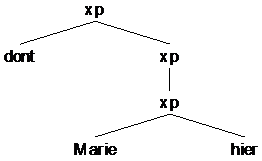
\includegraphics[width=\textwidth]{figures/chap3andconclusion16fevr17-img2.png}
\caption{Analyse en termes de fragment}
\label{ch3:fig2}
\end{figure} 

Comme mentionné dans la section~\ref{ch2:sect2.5.3.2}, un \isi{fragment} est une expression dont le contenu sémantique n’est pas déductible de la forme prise en isolation. Le contenu sémantique d’un \isi{fragment} dépend : (i) du type du \isi{fragment} ; (ii) du contenu sémantique des constituants du \isi{fragment} ; (iii) des informations contextuelles qui peuvent être de nature linguistique ou non \citep{GinzburgEtAl2000,FernandezEtAl2007}. 

 \largerpage 
Un \isi{fragment} phrastique, comme par exemple la \isi{question courte} \textit{quand} en \REF{ch3:ex112a}\footnote{Ce type d’ellipse est connu dans la littérature sous le nom de \is{Sluicing}\textit{sluicing}. Voir plus de détails sur cette construction dans la section~\ref{ch1:sect1.4.1.1}.}, est interprété comme ayant le même contenu sémantique que la phrase \textit{quand elle va venir} en \REF{ch3:ex112b}. Le contenu sémantique du \isi{fragment} \textit{quand} dans l’exemple \REF{ch3:ex112a} est une fonction (i) du type du \isi{fragment} (les \is{question courte}questions courtes ont le même type de contenu que les phrases interrogatives, {\cad} une abstraction propositionnelle), (ii) du contenu littéral du constituant dans le \isi{fragment} (\textit{quand} fournit le paramètre pour l’abstraction propositionnelle, en particulier il introduit un paramètre temporel) et (iii) de l’information contextuelle (la phrase source \textit{Marie va venir}, qui contient l’antécédent du \isi{fragment}, fournit la proposition dont on a besoin pour construire l’abstraction propositionnelle). Ainsi, le \isi{fragment} \textit{quand} a un contenu similaire à la phrase \textit{quand elle va venir}.  

\ea \label{ch3:ex112}
\ea 
Marie va venir, mais personne ne sait [quand]. \label{ch3:ex112a} 
\ex
Marie va venir, mais personne ne sait [quand elle va venir]. \label{ch3:ex112b}
\z 
\z

Pour calculer la sémantique du \isi{fragment}, on utilise le langage \is{Minimal Recursion Semantics (MRS)}\textit{Minimal Recursion Semantics} (désormais, MRS) de \citet{CopestakeEtAl2005}, car, outre le fait qu’il permet la description d’une sémantique «~plate~», il a l’avantage de permettre la description des représentations sémantiques partielles ou incomplètes (telles que celles d’un \isi{fragment} avant résolution), en sous-spécifiant les représentations complètes\footnote{ On a choisi \is{Minimal Recursion Semantics (MRS)}MRS, mais on pourrait utiliser aussi d’autres langages, comme \is{Lexical Resource Semantics (LRS)}\textit{Lexical Resource Semantics} (LRS, \citealt{RichterEtAl2004}) ou encore \is{Type Theory with Records (TTR)}\textit{Type Theory with Records} (TTR, \citealt{Cooper2005}).}. La résolution du \isi{fragment} consiste ainsi d'un système de méta-contraintes reliant quatre représentations sémantiques dont deux partielles : le contenu de la phrase hôte (= la source) et le contenu du \isi{fragment} résolu (= la cible) sont des représentations complètes, alors que le contenu «~abstrait~» obtenu à partir de l’hôte et le contenu des constituants du \isi{fragment} sont des représentations partielles.

En \is{Minimal Recursion Semantics (MRS)}MRS, les unités minimales de la représentation sémantique sont appelées des prédications élémentaires (angl. \textit{elementary predications}, abrégées EP). Elles représentent une relation sémantique accompagnée de ses arguments, p.ex. \textit{aimer(x, y)}. 


  
La représentation générale d’une structure \is{Minimal Recursion Semantics (MRS)}MRS est donnée en \REF{ch3:ex113}. Les traits qui nous intéressent ici sont les deux premiers. Le trait HOOK contient l’ensemble de l’information accessible de l’extérieur aux foncteurs sémantiques. En particulier, il contient le trait LTOP, qui enregistre le label sur lequel aucun autre n’a portée au niveau local (cela correspond à la tête sémantique de la structure qui est décrite), et le trait INDEX, qui enregistre l’indice de la relation accessible au foncteur. Le trait RELS est la liste de prédications élémentaires.

\newpage
\ea \label{ch3:ex113}
Structure générale MRS\\
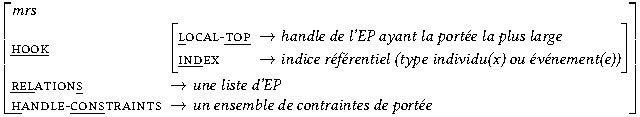
\includegraphics{figures/Ch3113.pdf}
 
\z

\largerpage
Les quatre représentations sémantiques dont on a besoin pour la résolution sémantique du \isi{fragment} dans les RSV correspondent à quatre listes de prédications élémentaires en \is{Minimal Recursion Semantics (MRS)}MRS : la liste \fbox{A} correspond au contenu de la phrase source (noté SOURCE par la suite) ; la liste \fbox{B} correspond au contenu abstrait (noté ABSTRACT-CONT) obtenu à partir de la phrase source ; la liste \fbox{C} représente le contenu du \isi{fragment} (noté FRAGMENT) et, enfin, la liste \fbox{D} correspond au contenu du \isi{fragment} résolu, appelé aussi la cible (noté TARGET). Cela est illustré en \REF{ch3:ex114} et décrit formellement en \REF{ch3:ex115}. Les listes \fbox{A} et \fbox{D} sont des représentations sémantiques complètes, alors que les listes \fbox{B} et \fbox{C} sont des représentations sémantiques partielles. 

\ea \label{ch3:ex114}
\ea 
Plusieurs personnes sont venues, [\textbf{dont} Marie hier]. \label{ch3:ex114a} 
\ex
Plusieurs personnes sont venues. (\fbox{A} = SOURCE) \label{ch3:ex114b} 
\ex 
X est venu (\fbox{B} = ABSTRACT-CONT) \label{ch3:ex114c}
\ex 
Marie hier (\fbox{C} = FRAGMENT) \label{ch3:ex114d}
\ex 
Marie est venue hier. (\fbox{D} = TARGET) \label{ch3:ex114e}
\z 
\z
 

   
\ea \label{ch3:ex115}
Représentation MRS du fragment en \REF{ch3:ex114}\\
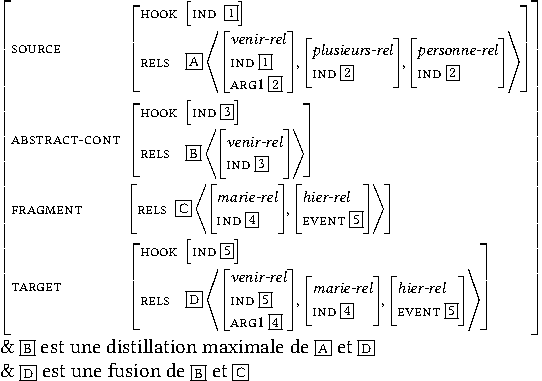
\includegraphics{figures/Ch3115.pdf} 
\z

Ces listes sont reliées par deux méta-contraintes : la fusion et la distillation\footnote{Je remercie Olivier Bonami pour m’avoir proposé ces deux termes.}, qui opèrent sur des prédications élémentaires du même type. 

\textbf{Fusion de listes :} Soient L\textsubscript{1}, L\textsubscript{2} et L\textsubscript{3} trois descriptions de listes. L\textsubscript{1} est une \textbf{fusion} de L\textsubscript{2} et L\textsubscript{3} si et seulement si chaque élément de L\textsubscript{1} est soit le résultat de l’unification d’un élément de L\textsubscript{2} avec un élément de L\textsubscript{3}, soit identique à un élément de L\textsubscript{2} ou de L\textsubscript{3}. Tout élément de L\textsubscript{2} ou L\textsubscript{3} doit apparaître dans L\textsubscript{1} soit tel quel, soit unifié à un élément de l’autre liste. 

\textbf{Distillation de listes :} Soient L\textsubscript{1}, L\textsubscript{2} et L\textsubscript{3} trois descriptions de listes. L\textsubscript{1} est une \textbf{distillation} de L\textsubscript{2} et L\textsubscript{3} si et seulement si (i) L\textsubscript{2} est une fusion de L\textsubscript{1} et L\textsubscript{2} et (ii) L\textsubscript{3} est une fusion de L\textsubscript{1} et L\textsubscript{3}.

\textbf{Distillation maximale de listes} : Soient L\textsubscript{1}, L\textsubscript{2} et L\textsubscript{3} trois descriptions de listes. L\textsubscript{1} est une \textbf{distillation maximale} de L\textsubscript{2} et L\textsubscript{3} si et seulement si (i) L\textsubscript{1} est une distillation de L\textsubscript{2} et L\textsubscript{3} et (ii) il n’existe pas de liste L\textsubscript{1}' qui soit une distillation de L\textsubscript{2} et L\textsubscript{3} et qui contienne plus d’éléments que L\textsubscript{1}.

La première contrainte opérant sur les quatre représentations sémantiques est donnée en \REF{ch3:ex115} ci-dessus : grosso modo, on fait la distillation du contenu de la source (liste \fbox{A}) et du contenu du \isi{fragment} résolu (liste \fbox{D}) afin de récupérer le contenu «~abstrait~» (liste \fbox{B}) dont on a besoin pour interpréter le \isi{fragment}. La distillation doit être maximale, afin de récupérer le maximum d’informations de la source (les RSV partagent tout avec leur hôte, excepté le contenu littéral du \isi{fragment}). Ainsi, le contenu de la cible en \REF{ch3:ex114e} ne peut pas être quelque chose de moins précis, comme \textit{Marie a fait quelque chose hier}. 

La deuxième contrainte qui s’ajoute en \REF{ch3:ex115} ci-dessus sert à obtenir le contenu du \isi{fragment} résolu (liste \fbox{D}) en fusionnant le contenu «~abstrait~» (liste \fbox{B}) et le contenu littéral du \isi{fragment} (liste \fbox{C}). A l’issue de la fusion, on obtient plusieurs résultats qui obéiront à des contraintes supplémentaires à l’interface syntaxe-sémantique, imposées par l’introducteur d’une RSV ou par la construction RSV elle-même.  

Ce système de représentation sémantique en \is{Minimal Recursion Semantics (MRS)}MRS peut être intégré dans une grammaire de type HPSG en utilisant un trait FRAGMENT dont la valeur correspond à deux traits : le trait SOURCE et le trait ABSTRACT-CONT qui sont de type \textit{sem-obj}. Dans l’approche qu’on adopte ici, la valeur du trait CONT de tous les signes est de type \textit{mrs}. Tous les signes possèdent également un trait C-CONT (\textit{constructional content}), permettant d’exprimer un éventuel contenu sémantique d’origine constructionnelle\footnote{ Les contenus de type \textit{message} y sont conçus comme des relations d’origine constructionnelle.}, la valeur de ce trait étant également de type \textit{mrs}. 

\ea \label{ch3:ex116}
Représentation du fragment en HPSG avec MRS (cas général)\\
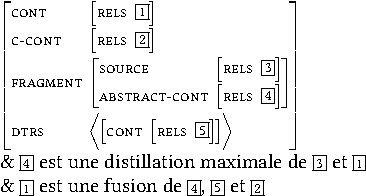
\includegraphics{figures/Ch3116.pdf}


% \noindent
% \begin{avm}
% [cont & [rels & @1]\\
%  c-cont &  [rels & @2]\\
%  fragment & [source &  [rels & @3]\\ 
%              abstract-cont & [rels & @4]]\\ 
%  dtrs & <[cont & [rels & @5]]>]
% \end{avm}\\
% \ \& \avmbox4 est une distillation maximale de \avmbox3 et \avmbox1\\ \& \avmbox1 est une fusion de \avmbox4, \avmbox5 et \avmbox2

\z

A la représentation du \isi{fragment} donnée en \REF{ch3:ex116}, on ajoute les deux contraintes mentionnées précédemment, qui peuvent être décrites comme suit : le contenu «~abstrait~» \fbox{4} est obtenu en distillant le contenu de la source \fbox{3} et le contenu du \isi{fragment} résolu \fbox{1}~; le contenu du \isi{fragment} résolu \fbox{1} est obtenu en fusionnant le contenu «~abstrait~» \fbox{4} avec les constituants du \isi{fragment} \fbox{5} et l’éventuel contenu sémantique d’origine constructionnelle \fbox{2}.  


\subsection{Théorie des clusters}\label{ch3:sect3.5.2}

Certains types de \is{fragment}fragments sont sujets à des contraintes de forme qui instancient les informations lexicales sur les propriétés de sous-catégorisation des items lexicaux qui ne sont pas réalisés dans la séquence elliptique. Cette propriété a amené \citet{GinzburgEtAl2000} à analyser le \isi{fragment} phrastique comme la branche unaire d’un syntagme ayant l’ensemble des propriétés d’une phrase, y compris la catégorie syntaxique VERBAL. Dans cette perspective, le \isi{fragment} \textit{Marie}, conçu comme une \isi{réponse courte} à une question comme \textit{Qui est venu?}, peut être décrit en postulant un syntagme de type tête-fragment, présenté en \REF{ch3:ex117} : 

\ea \label{ch3:ex117}
Syntagme de type tête-fragment dans \citet{GinzburgEtAl2000}\\
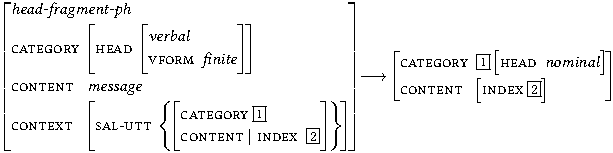
\includegraphics{figures/Ch3117.pdf}


% \noindent
% \begin{avm}
% [\tp{head-fragment-ph} \\
% category & [head & [\tp{verbal} \\ vform & finite]] \\
% content & message \\
% context & [sal-utt & \{[category @1 \\ content | index & @2]\}]] $\longrightarrow$ [category & @1 [head & nominal] \\ content & [index @2]]
% \end{avm}

\z

Cependant, l’approche que je présente ici est un peu différente de celle proposée par \citet{GinzburgEtAl2000}, car, contrairement aux types de \is{fragment}fragments \REF{ch3:ex118a} analysés par \citet{GinzburgEtAl2000}, les fragments dans les RSV \REF{ch3:ex119a} n’ont pas la même distribution que leurs contreparties à tête verbale, comme le montrent les différences d’acceptabilité qu’on observe avec les exemples en \REF{ch3:ex119}.

\ea \label{ch3:ex118}
\ea 
Je me demande [où]. \label{ch3:ex118a} 
\ex
Je me demande [où il est]. \label{ch3:ex118b}
\z 
\z 

\ea \label{ch3:ex119}
\ea 
Plusieurs ont parlé à mes amis, [dont Marie à Marc]. \label{ch3:ex119a} 
\ex
*Plusieurs \uline{ont parlé} à mes amis, [dont Marie \uline{a parlé} à Marc]. \label{ch3:ex119b}
\z 
\z

Cela est vrai même en dehors des constructions avec RSV. Il a été noté que les constructions elliptiques n’ont pas toujours la même distribution que leur source. Ainsi, en français la conjonction lexicalisée \textit{ainsi que} ou encore l’adverbial \textit{non pas} peuvent être suivis d’une séquence de syntagmes ayant le contenu d’une phrase comme en \REF{ch3:ex120a} et \REF{ch3:ex121a}, mais ils ne peuvent jamais se combiner avec une phrase finie telle qu'en \REF{ch3:ex120b} et \REF{ch3:ex121b}, cf. \citet{AbeilleEtAl1996} et \citet{Mouret2006,Mouret2007,Mouret2008}.

\ea \label{ch3:ex120}
 
\ea 
Paul a mangé une pomme, [\textbf{ainsi que} <Marie une orange>]. \label{ch3:ex120a} 
\ex
*Paul \uline{a mangé} une pomme, [\textbf{ainsi que} Marie \uline{a mangé} une orange]. \label{ch3:ex120b}
\z 
\z 

\ea \label{ch3:ex121}

\ea 
Paul a invité Marie [et \textbf{non pas} <Marie Paul>]. \label{ch3:ex121a} 
\ex
*Paul \uline{a invité} Marie [et \textbf{non pas} Marie \uline{a invité} Paul]. \label{ch3:ex121b}
\z 
\z

C’est pour cela qu’on choisit de représenter en \REF{ch3:ex122} les \is{fragment}fragments comme un sous-type de \textit{head-only-ph} dont la seule branche tête correspond à un \textit{cluster} (comme pour les constructions à gapping, analysées dans le chapitre~\ref{ch2}). Les \is{cluster}clusters sont des séquences de syntagmes qui ne sont pas reliés entre eux par des relations fonctionnelles. La notion de \isi{cluster} en HPSG a été proposée par \citet{Mouret2006,Mouret2007} pour rendre compte des coordinations de séquences (angl. \is{Argument Cluster Coordination (ACC)}\textit{Argument Cluster Coordination}) en français (voir aussi les sections~\ref{ch2:sect2.5.3.1} et~\ref{ch2:sect2.5.3.2}). Comme il l’indique, la notion de \isi{cluster} doit être définie indépendamment de la coordination dans la grammaire, vu le fait qu’elle est pertinente pour décrire non seulement des constructions apparaissant dans le domaine de la coordination, mais aussi de la subordination.

\ea \label{ch3:ex122}
Syntagme de type tête-fragment (nouvelle version)\\
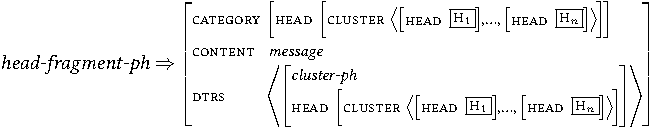
\includegraphics{figures/Ch3122.pdf}

% \noindent
% \textit{head-fragment-ph} $\Rightarrow$
% \begin{avm}
% [category & [head & [cluster & <[head & @{H$_1$}],..., [head & @{H$_n$}]>]] \\
% content & message\\
% dtrs & <[\tp{cluster-ph}\\ head & [cluster & <[head & @{H$_1$}],..., [head & @{H$_n$}]>]]>]
% \end{avm} 

\z

\citet{Mouret2006,Mouret2007} pose une construction spécifique \textit{cluster-ph} sans tête, qui est un sous-type de \textit{non-headed-ph}. Les syntagmes de type tête-fragment (\textit{head-fragment-ph}) et de type cluster (\textit{cluster-ph}) sont représentés dans la hiérarchie de syntagmes donnée en \figref{ch3:fig3}. 

\begin{figure}
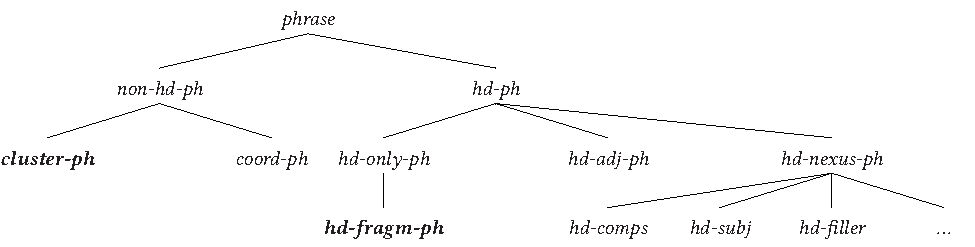
\includegraphics[width=\textwidth]{figures/Ch3Fig3.pdf} % \documentclass[12pt]{article}
\usepackage[latin1]{inputenc}
%\documentclass[twoside,14pt,a4paper]{article}
\usepackage{fullpage}
%\usepackage{times}
\usepackage{latexsym}
\usepackage{ecltree+}
\usepackage{avm}
\usepackage{avm+}
%\usepackage[utf8]{inputenc}
%\usepackage[francais]{babel}

\usepackage{combelow}

\usepackage{xyling}

\begin{document}


\noindent{\textbf{Figure 1 \hspace{1cm} Analyse par reconstruction syntaxique}}
\vspace{1mm}

\Tree[2]{         & \K{\textsc{s}}\B{dl}\B{dr}       & \\
              \K{dont} && \K{\textsc{s}}\B{dl}\B{d}     & \\
               & \K{\textsc{np}}\B{d} & \K{\textsc{vp}}\B{d}\B{dr}\B{drr} & &\\  
       & \K{Marie} & \K{$<$est$>$} & \K{$<$venue$>$} & \K{hier}}


\bigskip



\noindent{\textbf{Figure 2 \hspace{1cm} Analyse en termes de fragment}}
\vspace{1mm}

\Tree[2]{         & \K{\textsc{xp}}\B{dl}\B{dr} &\\  
               \K{dont} && \K{\textsc{xp}}\B{d}\\
       && \K{\textsc{xp}}\B{dl}\B{dr} &\\
      & \K{Marie} && \K{hier}}


\bigskip



\noindent{\textbf{Figure 3 \hspace{1cm} Hi\'erarchie de syntagmes en HPSG, incluant le fragment et le cluster}}
\noindent

\Tree[2] {&& \K[6.2]{\textit{phrase}}\Bkk{6.2,0}{0,0}{dl}\Bkk{6.2,0}{0,0}{drr}		\\
&\K{\textit{non-hd-ph}}\B{dl}\B{dr} &&& \K{\textit{hd-ph}}\B{dl}\B{dr}\B{drrr} \\ 
\K{\textbf{\textit{cluster-ph}}} & &  \K{\textit{coord-ph}} & \K{\textit{hd-only-ph}}\B{d} && \K{\textit{hd-adj-ph}} && \K{\textit{hd-nexus-ph}}\B{dll}\B{dl}\B{d}\B{dr}\\
& & & \K{\textbf{\textit{hd-fragm-ph}}} && \K{\textit{hd-comps}} & \K{\textit{hd-subj}} & \K{\textit{hd-filler}} & \K{\textit{...}}}


%\bigskip
\newpage



\noindent{\textbf{Figure 4 \hspace{1cm} Repr\'esentation simplifi\'ee d'un fragment contenant un cluster de deux constituants}}

\regAvmFonts\avmoptions{center}

\newcommand{\AVMXPone}{\begin{Avm}{XP}
        \[\tp{head-fragment-ph}\\ synsem & \@{2} \[head \@{1}\]\\ mrkg & nil \]
        \end{Avm} }
\newcommand{\AVMXPtwo}{\begin{Avm}{XP}
				\[\tp{cluster-ph} \\ synsem & \@{2} \[head \@{1} & \[cluster & \<\@{3}, \@{4} \> \] \] \] 
				\end{Avm}} 
\newcommand{\AVMNPone}{\begin{Avm}{NP}
    \[synsem & \@{3} \]
\end{Avm}}
\newcommand{\AVMNPtwo}{\begin{Avm}{NP}
    \[synsem & \@{4} \] 
    \end{Avm}}       
    

\smallAvmFonts
\begin{figure}[hbcd]
  \begin{center}
     \begin{bundle}{\AVMXPone}\setlength{\GapDepth}{40pt}
       \chunk[\textsc{hd}]{\setlength{\GapWidth}{45pt}
       		\begin{bundle}{\AVMXPtwo}
               \chunk[\textsc{n-hd}]{\setlength{\GapWidth}{70pt}\setlength{\GapDepth}{20pt}
                  \begin{bundle}{\AVMNPone}
                    \chunk{Marie}
                  \end{bundle}}
               \chunk[\textsc{n-hd}]{\setlength{\GapDepth}{20pt}
                  \begin{bundle}{\AVMNPtwo}
                    \chunk{hier}
                  \end{bundle}}
             \end{bundle}}
             
         \end{bundle}
       	      
    
  \end{center}
\end{figure}
\regAvmFonts


\newpage



\noindent{\textbf{Figure 5 \hspace{1cm} Repr\'esentation simplifi\'ee d'un fragment contenant un cluster unaire}}

\regAvmFonts\avmoptions{center}

\newcommand{\AVMXPthree}{\begin{Avm}{XP}
        \[\tp{head-fragment-ph}\\ synsem & \@{2} \[head \@{1}\]\\ mrkg & nil \]
        \end{Avm} }
\newcommand{\AVMXPfour}{\begin{Avm}{XP}
				\[\tp{cluster-ph} \\ synsem & \@{2} \[head \@{1} & \[cluster & \<\@{3}NP \> \] \] \] 
				\end{Avm}} 
\newcommand{\AVMNPthree}{\begin{Avm}{NP}
    \[synsem & \@{3} \]
\end{Avm}}
          

\smallAvmFonts
\begin{figure}[hbcd]
  \begin{center}
     \begin{bundle}{\AVMXPthree}\setlength{\GapDepth}{40pt}
       \chunk[\textsc{hd}]{\setlength{\GapWidth}{45pt}
       		\begin{bundle}{\AVMXPfour}
               \chunk[\textsc{n-hd}]{\setlength{\GapWidth}{70pt}\setlength{\GapDepth}{20pt}
                  \begin{bundle}{\AVMNPthree}
                    \chunk{Marie}
                  \end{bundle}}
               
             \end{bundle}}
             
         \end{bundle}
       	      
    
  \end{center}
\end{figure}
\regAvmFonts


\bigskip



\noindent{\textbf{Figure 6 \hspace{1cm} Relations fonctionnelles possibles dans la RSV}
\vspace{1mm}

\noindent
\Tree{ &&& \K{\textsc{xp}}\B{dll}_{?}\B{drr}^{HD}  &&&\\
          & \K{\textsc{pp}}\B{dl}\B{dr} & && & \K{\textsc{xp}}\B{d} &\\                         
\K{dintre} && \K{care} &&& \K{\textsc{xp}}\B{dl}\B{dr}\\
&&&&      \K{una} && \K{ieri}}

\paragraph{}

\Tree{&&& \K{\textsc{pp}}\B{dll}_{HD}\B{drr}^{?} &&&\\
          & \K{\textsc{pp}}\B{dl}\B{dr} & && & \K{\textsc{xp}}\B{d} &\\                         
\K{dintre} && \K{care} &&& \K{\textsc{xp}}\B{dl}\B{dr}\\
&&&&      \K{una} && \K{ieri}}

\paragraph{}

\Tree{&&& \K{\textsc{xp}}\B{dll}_{N-HD}\B{drr}^{N-HD} &&&\\
       & \K{\textsc{pp}}\B{dl}\B{dr} & && & \K{\textsc{xp}}\B{d} &\\                         
\K{dintre} && \K{care} &&& \K{\textsc{xp}}\B{dl}\B{dr}\\
&&&&      \K{una} && \K{ieri}}


\bigskip



\noindent{\textbf{Figure 7 \hspace{1cm} Le syntagme de type t\^ete-foncteur dans une hi\'erarchie de syntagmes}

\noindent
\Tree[2]{ & \K[5.2]{\textit{phrase}}\Bkk{5.2,0}{0,0}{dl}\Bkk{5.2,0}{0,0}{dr}		\\
\K{\textit{non-hd-ph}}	&			 & \K[5.2]{\textit{hd-ph}}\Bkk{5.2,0}{0,0}{dl}\Bkk{5.2,0}{0,0}{dr}\Bkk{5.2,0}{0,0}{drrrr}  \\
& \K{\textit{hd-only-ph}}\B{d} & &   \K{\textit{hd-adj-ph}}\B{d}\B{dr} &&& \K{\textit{hd-nexus-ph}}\B{dl}\B{dr}\B{drr}\\
& \K{\textit{hd-fragm-ph}} && \K{\textbf{\textit{hd-funct-ph}}} & \K{\textit{...}} & \K{\textit{hd-comps-ph}} && \K{\textit{hd-subj-ph}} & \K{\textit{...}}}


\bigskip



\noindent{\textbf{Figure 8 \hspace{1cm} Arbre avec un syntagme t\^ete-foncteur}}

\regAvmFonts\avmoptions{center}
\newcommand{\AVMXPfive}{\begin{Avm}{XP}
        \[\tp{head-functor-ph}\\ head & \@{1}\\ mrkg & \@{2} marked\]
      									\end{Avm}}
\newcommand{\AVMPPone}{\begin{Avm}{PP}
        \[cat & \[head & \[select & \@{3}\]\\ mrkg & \@{2}\]\]
      									\end{Avm}}
\newcommand{\AVMXPsix}{\begin{Avm}{XP}
  \@{3}\[cat & \[head & \@{1}\\ mrkg & unmarked\]\]
      									\end{Avm}}
\newcommand{\AVMXPsixbis}{\begin{Avm}{XP} 
        							 \end{Avm}}
\newcommand{\AVMNPfirst}{\begin{Avm}{NP} 
        							 \end{Avm}}


\smallAvmFonts
\begin{figure}[hbcd]
  \begin{center}\setlength{\GapWidth}{60pt}\setlength{\GapDepth}{30pt}
     \begin{bundle}{\AVMXPfive}     	  			
     \chunk[\textsc{fct}]{\setlength{\GapWidth}{60pt}\setlength{\GapDepth}{20pt}
         \begin{bundle}{\AVMPPone}
           \chunk{parmi}
           \chunk{lesquelles}
         \end{bundle}}
     
  		\chunk[\textsc{hd}]{\setlength{\GapWidth}{60pt}\setlength{\GapDepth}{15pt}
         \begin{bundle}{\AVMXPsix}
         	\chunk{\setlength{\GapDepth}{15pt}\begin{bundle}{\AVMXPsixbis}
         	 \chunk{\setlength{\GapDepth}{15pt}\begin{bundle}{\AVMNPfirst}
           \chunk{Marie}
           \end{bundle}}
           \end{bundle}}  
         \end{bundle}}
 
     \end{bundle}
         
  \end{center}
\end{figure}
\regAvmFonts


\newpage



\noindent{\textbf{Figure 9 \hspace{1cm} Syntaxe simplifi\'ee des constructions \`a RSV en fran\c{c}ais}}

\Tree{ &&& \K{\textsc{s}}\B{dll}_{HD}\B{drrr}^{ADJ}  &&\\
& \K{\textsc{s}}\B{dl}_{SUBJ}\B{dr}^{HD} & && && \K{\textsc{xp}}\B{dl}_{FCT}\B{drr}^{HD} &\\ 
\K{\textsc{np}}\TRi && \K{\textsc{v}}\B{d} &&& \K{\textsc{pp}}\B{dl}_{HD}\B{dr}^{COMPS} & && \K{\textsc{xp}}\B{d}^{HD} &\\
\K{plusieurs}\Below{personnes} && \K{chantent} && \K{\textsc{p}rep}\B{d} && \K{\textsc{np}}\TRi && \K{\textsc{xp}}\B{d}^{N-HD}\\
&&&& \K{parmi} && \K{lesquelles} && \K{\textsc{np}}\TRi\\
&&&& && & & \K{Marie}}


\bigskip



\noindent{\textbf{Figure 10 \hspace{1cm} Syntaxe simplifi\'ee des constructions \`a RSV en roumain}}

\Tree{ &&& \K{\textsc{s}}\B{dll}_{HD}\B{drrr}^{ADJ}  &&\\
& \K{\textsc{s}}\B{dl}_{HD}\B{dr}^{SUBJ} & && && \K{\textsc{xp}}\B{dl}_{FCT}\B{drr}^{HD} &\\ 
\K{\textsc{v}}\B{d} && \K{\textsc{np}}\TRi &&& \K{\textsc{pp}}\B{dl}_{HD}\B{dr}^{COMPS} & && \K{\textsc{xp}}\B{d}^{HD} &\\
\K{vin} && \K{mai}\Below{multe}\Below{persoane} && \K{\textsc{p}rep}\B{d} && \K{\textsc{np}}\TRi && \K{\textsc{xp}}\B{d}^{N-HD}\\
&&&& \K{printre} && \K{care} && \K{\textsc{np}}\TRi\\
&&&& && & & \K{\c{s}i Maria}}

  
\newpage



\noindent{\textbf{Figure 11 \hspace{1cm} Relation \`a distance entre l'introducteur et l'\'el\'ement distingu\'e: accessibilit\'e de l'\'el\'ement distingu\'e dans le corps de la RSV}}      									      				

\regAvmFonts\avmoptions{center}
\newcommand{\AVMXPseven}{\begin{Avm}{XP}
        \[\tp{head-functor-ph} \\ ss & \[ head & \@{6} noun \\ mrkg & \@{7} \\ rel & \{\@{4}\} \] \] 
        									\end{Avm}}
        									
\newcommand{\AVMPPtwo}{\begin{Avm}{PP}
        \[\tp{head-comps-ph} \\ ss & \[ head & \[select & \@{1}  \] \\ mrkg & \@{7}\\ rel & \{\@{4}\} \] \] 
        							 \end{Avm}}
        							 
\newcommand{\AVMPrepone}{\begin{Avm}{Prep}
  			\[cat & \[head & \[select & \@{1} \[cont & \[anchors & \<\[ind & \@{3}\]\>\]\]\] \\ mrkg & \@{7}\\ val & \[comps & \<\@{2}\>\] \\ arg-st & \<\@{1}, \@{2}\> \] \\
  			  cont & \[ltop & \@{5} \\ rels & \<\[\tp{sum-subpart-rel} \\ label & \@{5} \\ subpart & \@{3} \\ sum & \@{4} \] \> \] \]
      									\end{Avm}}
      									
\newcommand{\AVMNPfour}{\begin{Avm}{NP}
   \[ss &\@{2}\[cat & \[head & noun\]\\ cont & \[ind & \@{4}\] \\ rel & \{\@{4}\}\] \]
        							 \end{Avm}}

\newcommand{\AVMXPeight}{\begin{Avm}{XP}
   \[\tp{head-fragment-ph} \\ ss &\@{1}\[cat & \[head & \@{6} noun\]\\ cont & \[ind & \@{3}\] \]\] 
        							 \end{Avm}}
        							 
\newcommand{\AVMXPeightbis}{\begin{Avm}{XP} 
        							 \end{Avm}}
\newcommand{\AVMNPsecond}{\begin{Avm}{NP} 
        							 \end{Avm}}        							 

\smallAvmFonts
\begin{figure}[hbcd]
  \begin{center}\setlength{\GapWidth}{100pt}\setlength{\GapDepth}{30pt}
     \begin{bundle}{\AVMXPseven}     	  			
   		\chunk[\textsc{fct}]{\setlength{\GapWidth}{140pt}\setlength{\GapDepth}{20pt}
         \begin{bundle}{\AVMPPtwo}
         	 \chunk[\textsc{hd}]{
         	 	\begin{bundle}{\AVMPrepone}
           		\chunk{parmi}
         		 \end{bundle}}
         	  \chunk[\textsc{comps}]{
         	 	 \begin{bundle}{\AVMNPfour}
           	 	\chunk{lesquelles}
         		 \end{bundle}}
         	\end{bundle}}
       \chunk[\textsc{hd}]{\setlength{\GapDepth}{15pt}
         	 	 \begin{bundle}{\AVMXPeight}
           	 	\chunk{\setlength{\GapDepth}{15pt}\begin{bundle}{\AVMXPeightbis}
         	 \chunk{\setlength{\GapDepth}{15pt}\begin{bundle}{\AVMNPsecond}
           \chunk{Marie}
           \end{bundle}}
           \end{bundle}}
         		 \end{bundle}}
      \end{bundle}
         
  \end{center}
\end{figure}
\regAvmFonts


\newpage



\noindent{\textbf{Figure 12 \hspace{1cm} Relation \`a distance entre la RSV et son ant\'ec\'edent: accessibilit\'e de l'ant\'ec\'edent dans la phrase h\^ote}}

\regAvmFonts\avmoptions{center}
\newcommand{\AVMSone}{\begin{Avm}{S}
        \[\tp{head-functor-ph}\] 
       							 \end{Avm}}
        							 
\newcommand{\AVMStwo}{\begin{Avm}{S}
   \[ss & \@{2}\[cont & \[ind & \@{6} \\ rels & \@{9}\] \] \]
        							 \end{Avm}}
        							 
\newcommand{\AVMNPfive}{\begin{Avm}{NP$_i$}
    	 \[cont & \[ind & \@{4}\] \] 
        							 \end{Avm}}

\newcommand{\AVMVone}{\begin{Avm}{V} 
        							 \end{Avm}}
        							         							 
\newcommand{\AVMXPnine}{\begin{Avm}{XP}
        \[ss & \[cat & \[head & \@{1} \[select & \@{2}\[ cont \[ anchors & \<\[ind & \@{4}\]\>\]\]\] \\
         mrkg & \@{10} \] \\
         cont & \[ind & \@{7}\]\\
         c-cont & \[rels & \<\[\tp{sum-subpart-rel}\\ 
         											subpart & \@{7} event\\
         											sum & \@{6} event\]\>\] \\
											rel & \{\@{4}\}\] \]
        									\end{Avm}}
        									        							 
\newcommand{\AVMPPthree}{\begin{Avm}{PP}
  			 \[ss &\[cat & \[head & \[select & \@{3} \] \\
         mrkg & \@{10} \]\\
			cont & \[ltop & \@{5} \\ rels & \<\[\tp{sum-subpart-rel} \\ label & \@{5} \\ subpart & \@{8} \\ sum & \@{4} \] \> \] \\
			rel & \{\@{4}\}\] \]
      									\end{Avm}}
      									
\newcommand{\AVMXPten}{\begin{Avm}{XP}
   			\[ss &\@{3}\[cat \[head & \@{1}\] \\ 
			cont \[ind  \@{7}\\
   								anchors & \<\[ind & \@{8}\]\>\]\\
   				fragment \[source \[ind & \@{6} \\ rels & \@{9}\]\\
   										abstract-cont \@{B}\]\] \]
        							 \end{Avm}}

\newcommand{\AVMXPtenbis}{\begin{Avm}{XP} 
        							 \end{Avm}}
\newcommand{\AVMNPthird}{\begin{Avm}{NP} 
        							 \end{Avm}}

\smallAvmFonts
\begin{figure}[hbcd]
  \begin{center}\setlength{\GapDepth}{25pt}
     \begin{bundle}{\AVMSone}     	  			
   		\chunk[\textsc{hd}]{
         \begin{bundle}{\AVMStwo}
         	 \chunk[\textsc{subj}]{
         	 	\begin{bundle}{\AVMNPfive}
           		\chunk{plusieurs personnes}
         		 \end{bundle}}
    
         	  \chunk[\textsc{hd}]{
         	 	 \begin{bundle}{\AVMVone}
           	 	\chunk{chantent}
         		 \end{bundle}}
         		 \end{bundle}}
         	
     \chunk[\textsc{fct}]{\setlength{\GapWidth}{110pt}\setlength{\GapDepth}{30pt}
       \begin{bundle}{\AVMXPnine}
         	\chunk[\textsc{fct}]{\setlength{\GapWidth}{30pt}
         	 	\begin{bundle}{\AVMPPthree}
           		\chunk{parmi}
           		\chunk{lesquelles$_i$}
         		 \end{bundle}}
          \chunk[\textsc{hd}]{\setlength{\GapWidth}{20pt}\setlength{\GapDepth}{15pt}
         	 	\begin{bundle}{\AVMXPten}
           	 	\chunk{\setlength{\GapDepth}{15pt}\begin{bundle}{\AVMXPtenbis}
         	 \chunk{\setlength{\GapDepth}{15pt}\begin{bundle}{\AVMNPthird}
           \chunk{Marie}
           \end{bundle}}
           \end{bundle}}
         		 \end{bundle}}	 
         	 \end{bundle}}
         	 	
        \end{bundle}
         
  \end{center}
\end{figure}
\regAvmFonts


\newpage



\noindent{\textbf{Figure 13 \hspace{1cm} Arbre avec le compl\'ementeur \textit{dont} dans les relatives ordinaires}}

\regAvmFonts\avmoptions{center}

\newcommand{\AVMNPsix}{\begin{Avm}{NP}
        \[\tp{head-functor-ph}\]
      \end{Avm}}
\newcommand{\AVMNPseven}{\begin{avm} \@1NP$_i$
      \end{avm}}
\newcommand{\AVMSthree}{\begin{Avm}{S}
    \[head & \[select & \@{1} \] \\ mrkg & dont \\ slash & \{ \} \] 
    \end{Avm}}
\newcommand{\AVMCompr}{\begin{Avm}{Compr}
    \[head & \[vform & \@{2}\]\\ mrkg & dont \\ comps & \<\@{3}\>\\ bind & \{\@{4}\} \\ slash & \{\} \]
		\end{Avm}}
\newcommand{\AVMSfour}{\begin{Avm}{S}
\@{3}\[vform & \@{2} tensed \\ subj & \< \>\\ slash & \{\@{4}PP$_i$[\textit{de}] \}\\ mrkg & unmarked \]
\end{Avm}}
\newcommand{\AVMNPeight}{\begin{Avm}{NP}
    \end{Avm}}
\newcommand{\AVMVtwo}{\begin{Avm}{V}
		\[slash & \{\@{4}\}\]
    \end{Avm}}
    
\smallAvmFonts
\begin{figure}[hbcd]

\begin{center}\setlength{\GapWidth}{40pt}\setlength{\GapDepth}{20pt}
     \begin{bundle}{\AVMNPsix}
     
\chunk[\textsc{hd}]{\setlength{\GapDepth}{30pt}
			\begin{bundle}{\AVMNPseven}
               \chunk{l'histoire}
               \end{bundle}
         }

\chunk[\textsc{fct}]{\setlength{\GapWidth}{80pt}\setlength{\GapDepth}{20pt}
         \begin{bundle}{\AVMSthree}
           \chunk[\textsc{hd}]{
             \begin{bundle}{\AVMCompr}
             		\chunk{dont}
               		\end{bundle}
        			 }
             
               \chunk[\textsc{comps}]{
                  \begin{bundle}{\AVMSfour}
                    \chunk[\textsc{subj}]{
                      \begin{bundle}{\AVMNPeight}
                      \chunk{Marie}
               		\end{bundle}
        			 }
                  
               \chunk[\textsc{hd}]{
                  \begin{bundle}{\AVMVtwo}
                    \chunk{parle}
                  \end{bundle}}
             \end{bundle}
           }
         \end{bundle}
       }
     
     \end{bundle}
  \end{center}
\end{figure}
\regAvmFonts


\newpage



\noindent{\textbf{Figure 14 \hspace{1cm} Arbre avec l'introducteur \textit{dont} dans les RSV}}

\regAvmFonts\avmoptions{center}
\newcommand{\AVMSfive}{\begin{Avm}{S}
        \[\tp{head-functor-ph}\] 
       							 \end{Avm}}
        							 
\newcommand{\AVMSsix}{\begin{Avm}{S}
    \[\tp{head-subject-ph} \\ ss & \@{2}\[cont & \[ind & \@{6}\] \] \]
        							 \end{Avm}}
        							 
\newcommand{\AVMNPnine}{\begin{Avm}{NP}
    	 \[ss & \[cont & \[ind & \@{4}\] \] \] 
        							 \end{Avm}}

\newcommand{\AVMVthree}{\begin{Avm}{V} 
        							 \end{Avm}}
        							         							 
\newcommand{\AVMXPeleven}{\begin{Avm}{XP}
        \[\tp{head-functor-ph} \\ ss & \[cat & \[head \@{1} & \[select & \@{2} \] \\ mrkg & dont \] \] \]
        									\end{Avm}}
        									        							 
\newcommand{\AVMYPone}{\begin{Avm}{?P}
  			\[ss & \[cat & \[head & \[select & \[cat \[head \| select \@{7} \| cont \[anchors & \<\[ind & \@{4}\]\> \] \] \\ cont \[anchors & \<\[ind & \@{3}\]\> \] \] \] \\ mrkg & dont\] \\
  			cont & \[ltop & \@{5} \\ rels & \<\[\tp{sum-subpart-rel} \\ label & \@{5} \\ subpart & \@{3} \\ sum & \@{4} \] \> \] \] \]
      									\end{Avm}}
      									
\newcommand{\AVMXPtwelve}{\begin{Avm}{XP}
   \[\tp{head-fragment-phrase}\\ ss & \@{7}\[cat & \[head & \@{1}\] \\ cont & \[ind & \@{3}\]\] \]
        							 \end{Avm}}

\newcommand{\AVMXPtwelvebis}{\begin{Avm}{XP} 
        							 \end{Avm}}
\newcommand{\AVMNPfourth}{\begin{Avm}{NP} 
        							 \end{Avm}}

\smallAvmFonts
\begin{figure}[hbcd]
  \begin{center}\setlength{\GapWidth}{50pt}\setlength{\GapDepth}{25pt}
     \begin{bundle}{\AVMSfive}     	  			
   		\chunk[\textsc{hd}]{\setlength{\GapWidth}{10pt}
         \begin{bundle}{\AVMSsix}
         	 \chunk[\textsc{subj}]{\setlength{\GapDepth}{15pt}
         	 	\begin{bundle}{\AVMNPnine}
           		\chunk{plusieurs personnes}
         		 \end{bundle}}
    
         	  \chunk[\textsc{hd}]{\setlength{\GapDepth}{19pt}
         	 	 \begin{bundle}{\AVMVthree}
           	 	\chunk{chantent}
         		 \end{bundle}}
         		 \end{bundle}}
         	
     \chunk[\textsc{fct}]{\setlength{\GapWidth}{200pt}\setlength{\GapDepth}{80pt}
       \begin{bundle}{\AVMXPeleven}
         	\chunk[\textsc{fct}]{\setlength{\GapWidth}{100pt}\setlength{\GapDepth}{40pt}
         	 	\begin{bundle}{\AVMYPone}
           		\chunk{dont}
         		 \end{bundle}}
          		\chunk[\textsc{hd}]{\setlength{\GapWidth}{130pt}\setlength{\GapDepth}{15pt}
         	 	\begin{bundle}{\AVMXPtwelve}
           	 	\chunk{\setlength{\GapDepth}{15pt}
           	 	\begin{bundle}{\AVMXPtwelvebis}
         	 \chunk{\setlength{\GapDepth}{15pt}
         	 \begin{bundle}{\AVMNPfourth}
           \chunk{Marie}
           \end{bundle}}
           \end{bundle}}
         		 \end{bundle}}	 
         	 \end{bundle}}
         	 	
        \end{bundle}
         
  \end{center}
\end{figure}
\regAvmFonts


\end{document}
%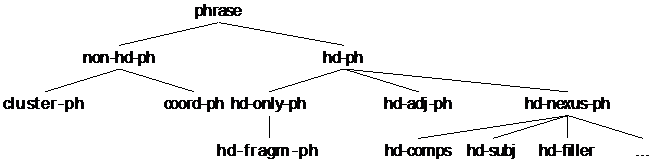
\includegraphics[width=\textwidth]{figures/chap3andconclusion16fevr17-img8.png}
\caption{Hiérarchie de syntagmes en HPSG, incluant le fragment et le cluster}
\label{ch3:fig3}
\end{figure} 

Le syntagme de type \isi{cluster}, défini formellement en \REF{ch3:ex123}\footnote{Pour plus de détails sur les contraintes du syntagme \textit{cluster-ph}, voir la représentation complète donnée en \REF{ch2:ex262} dans la section~\ref{ch2:sect2.5.3.1}.}, présente un trait de tête CLUSTER qui prend pour valeur la liste des \textit{synsem} associées aux constituants immédiats. Les propriétés syntaxiques et sémantiques de ses constituants sont ainsi rendues accessibles au niveau de la construction. Le \isi{cluster} peut comporter un seul constituant immédiat ou plus. 

\ea \label{ch3:ex123}
Syntagme de type cluster (cf. \citealt{Mouret2006,Mouret2007})\\
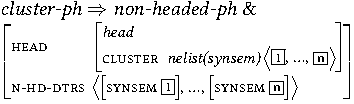
\includegraphics{figures/Ch3123.pdf}

% \noindent
% \textit{cluster-ph} $\Rightarrow$ \textit{non-headed-ph} \& \\
% \begin{avm}
% [head & [\tp{head}\\
% 				 cluster & nelist\(synsem\) <@{1}, ..., @{n}>]\\
%  n-hd-dtrs & <[synsem @{1}], ..., [synsem @{n}]>]
 
% \end{avm}

\z

A partir de cette définition du syntagme \isi{cluster}, on considère que les RSV dont le corps contient un seul syntagme présentent un \isi{cluster} unaire, ce qui nous permet de généraliser l’analyse de façon simplifiée. On va subsumer donc sous la même analyse les deux formes de réalisation du corps des RSV, décrites dans la section~\ref{ch3:sect3.2.2}. 

\largerpage[-2]
\begin{figure}
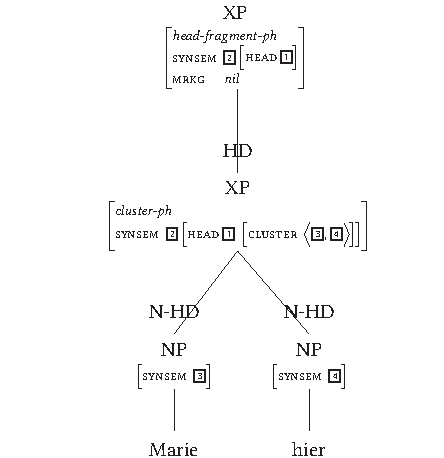
\includegraphics{figures/Ch3Fig4.pdf}  
\caption{Représentation simplifiée d’un fragment contenant un cluster de deux constituants}
\label{ch3:fig4}
\end{figure}

\begin{figure}
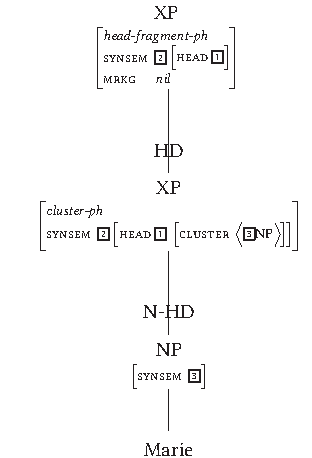
\includegraphics{figures/Ch3Fig5.pdf} 
\caption{Représentation simplifiée d’un fragment contenant un cluster unaire}
\label{ch3:fig5}
\end{figure}

Une fois les deux syntagmes définis (\textit{hd-fragment-ph} et \textit{cluster-ph}), on peut représenter formellement le corps de la RSV sous ses deux formes. Ainsi, \figref{ch3:fig4} est la représentation simplifiée d’un corps contenant un \isi{cluster} de deux constituants, alors que \figref{ch3:fig5} est la représentation d’un corps contenant un \isi{cluster} unaire. Le syntagme «~supérieur~» (\textit{head-fragment-ph}) hérite du syntagme «~inférieur~» (\textit{cluster-ph}) sa catégorie sous-spécifiée, lui permettant de se combiner avec des foncteurs qui sélectionnent une catégorie non finie, comme c’est le cas de la conjonction \textit{ainsi que} ou encore de l’averbial \textit{non pas} présentés plus haut et exemplifiés en \REF{ch3:ex120} et \REF{ch3:ex121}.




A ne pas confondre les notions de \is{fragment}\textit{fragment} et \is{cluster}\textit{cluster~}: la notion de \is{cluster}\textit{cluster} est une notion syntaxique, liée à la constituance, alors que la notion de \is{fragment}\textit{fragment} est une notion plutôt sémantique, liée au fait que l’interprétation n’est pas autonome~; elle dépend de l’interprétation de l’antécédent.


\subsection{Relations fonctionnelles dans la RSV}\label{ch3:sect3.5.3}
\largerpage[-1]
On s’intéresse maintenant aux relations fonctionnelles qui s’établissent entre le corps de la RSV et l’introducteur. Avant de lister les analyses envisageables pour la RSV, je veux présenter les grandes lignes de l’analyse proposée par \citet{Godard1988} et \citet{AbeilleEtAl2006,AbeilleEtAl2007} pour les relatives ordinaires du français. Deux grands types de relatives sont distingués en fonction du type d’introducteur : les relatives avec pronom relatif (\textit{pro-rel-clause}) et les relatives avec complémenteur (\textit{compr-rel-clause})\footnote{ Parmi ces dernières, on distingue \REF{ch3:fn22i} les relatives avec gap (introduites par \textit{que / qui} ou \textit{dont}) des \REF{ch3:fn22ii} relatives sans gap (en \textit{que / qui}). Comme les formes \textit{que} et\textit{ qui} ne sont pas employées dans les RSV, on s’intéresse ici uniquement aux relatives en \textit{dont}, donc on laisse de côté la discussion sur les relatives sans gap, qui par ailleurs relèvent du français parlé (pour plus de détails et exemples liés à ce type spécifique, voir \citealt{AbeilleEtAl2006}).

\ea \label{ch3:fn22i}
\ea quelque chose [\textbf{que} je regarde]
\ex quelqu’un [\textbf{qui} chante]
\ex quelqu’un [\textbf{dont} on parle]
\z
\z

\ea \label{ch3:fn22ii} 
\ea une fille [\textbf{qu}’elle est sympa]
\ex des feux [\textbf{qu}’il faut appeler les pompiers]
\z
\zlast}. Un exemple simplifié pour chaque type est donné en \REF{ch3:ex124}. 


\ea \label{ch3:ex124}
\ea 
une personne [\textbf{à laquelle} on parle] \label{ch3:ex124a} 
\ex
une personne [\textbf{dont} on parle] \label{ch3:ex124b} 
\z 
\z

Les relatives à pronom relatif comme \REF{ch3:ex124a} sont analysées comme des cons\-tructions à \isi{extraction} ; dans cette configuration, l’introducteur \textit{à laquelle} a la fonction extrait (angl. \textit{filler}) et doit correspondre à un gap dans le reste de la relative. Ce sous-type de relative contraint le syntagme extrait à être un syntagme prépositionnel contenant un pronom relatif. Ces relatives sont donc analysées comme des syntagmes de type tête-extrait (angl. \textit{head-filler-ph}, cf. la hiérarchie donnée en \figref{ch3:fig3}). En ce qui concerne le deuxième sous-type de relatives, {\cad} celles avec complémenteur, elles sont analysées plutôt comme des syntagmes de type tête-complément (angl. \textit{head-complement-ph}). Ainsi, le complémenteur \textit{dont}\footnote{Voir les propriétés du complémenteur \textit{dont} présentées dans la section~\ref{ch3:sect3.2.1.2}.} en \REF{ch3:ex124b} est analysé comme une tête syntaxique prenant une phrase comme complément et introduisant un trait syntaxique MARKING (abrégé MRKG dans les structures de traits en HPSG) qui sert à distinguer les relatives avec et sans complémenteur.

On observe donc que pour les relatives ordinaires on n’a pas d’analyse uniforme en français. Revenant aux RSV, on doit préciser que ces relatives sans verbe ne se prêtent a priori à aucune des deux analyses proposées pour les relatives verbales en français, car il n’y a pas de gap dans la RSV, {\cad} il n’y a pas d’élément manquant (en position canonique) correspondant à l’introducteur. Aucune relation \is{extraction}d’extraction ne semble exister au sein des RSV. De plus, comme on l’a observé dans la section~\ref{ch3:sect3.2.1.2}, la forme \textit{dont} dans les RSV n’a pas exactement les mêmes propriétés que le complémenteur \textit{dont} dans les relatives ordinaires. Par conséquent, on doit chercher d’autres possibilités d’analyse pour les RSV. 

On commence d’abord à distinguer le constituant qui pourrait avoir la fonction de tête dans la RSV. Il y a trois analyses possibles : (i) soit c’est le corps de la RSV qui est la tête (analyse A, cf. \figref{ch3:fig6a}), (ii) soit c’est l’introducteur de la RSV qui est la tête (analyse B, cf. \figref{ch3:fig6b}), (iii) soit il n’y a pas de tête (analyse C, cf \figref{ch3:fig6c}). On montre par la suite que les analyses B et C doivent être éliminées, car le corps de la RSV présente des propriétés de tête. 

% \begin{multicols}{2}
% Analyse A : Le corps est la tête.\\
% %   \begin{forest}
% %    [XP [PP, edge label={node[midway,left,font=\scriptsize]{?}} [dintre] [care] ]  [XP, edge label={node[midway,right,font=\scriptsize]{HD}} [XP [una] [ieri] ] ] ] 
% %   \end{forest}\vspace{\baselineskip}

  
%   Analyse C : Il n’y a pas de tête.\\
% % \begin{forest}
% %     [XP [PP, edge label={node[midway,left,font=\scriptsize]{N-HD}} [dintre] [care] ]  [XP, edge label={node[midway,right,font=\scriptsize]{N-HD}} [XP [una] [ieri] ] ] ] 
% %   \end{forest}\columnbreak

  
% Analyse B : L’introducteur est la tête.\\
% %   \begin{forest}
% %     [XP [PP, edge label={node[midway,left,font=\scriptsize]{HD}} [dintre] [care] ]  [XP, edge label={node[midway,right,font=\scriptsize]{?}} [XP [una] [ieri] ] ] ] 
% %   \end{forest}

% \end{multicols}

\begin{figure}
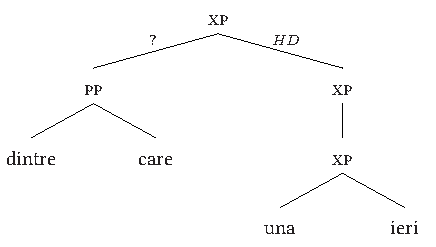
\includegraphics{figures/Ch3Fig6a.pdf} % \documentclass[12pt]{article}
\usepackage[latin1]{inputenc}
%\documentclass[twoside,14pt,a4paper]{article}
\usepackage{fullpage}
%\usepackage{times}
\usepackage{latexsym}
\usepackage{ecltree+}
\usepackage{avm}
\usepackage{avm+}
%\usepackage[utf8]{inputenc}
%\usepackage[francais]{babel}

\usepackage{combelow}

\usepackage{xyling}

\begin{document}


\noindent{\textbf{Figure 1 \hspace{1cm} Analyse par reconstruction syntaxique}}
\vspace{1mm}

\Tree[2]{         & \K{\textsc{s}}\B{dl}\B{dr}       & \\
              \K{dont} && \K{\textsc{s}}\B{dl}\B{d}     & \\
               & \K{\textsc{np}}\B{d} & \K{\textsc{vp}}\B{d}\B{dr}\B{drr} & &\\  
       & \K{Marie} & \K{$<$est$>$} & \K{$<$venue$>$} & \K{hier}}


\bigskip



\noindent{\textbf{Figure 2 \hspace{1cm} Analyse en termes de fragment}}
\vspace{1mm}

\Tree[2]{         & \K{\textsc{xp}}\B{dl}\B{dr} &\\  
               \K{dont} && \K{\textsc{xp}}\B{d}\\
       && \K{\textsc{xp}}\B{dl}\B{dr} &\\
      & \K{Marie} && \K{hier}}


\bigskip



\noindent{\textbf{Figure 3 \hspace{1cm} Hi\'erarchie de syntagmes en HPSG, incluant le fragment et le cluster}}
\noindent

\Tree[2] {&& \K[6.2]{\textit{phrase}}\Bkk{6.2,0}{0,0}{dl}\Bkk{6.2,0}{0,0}{drr}		\\
&\K{\textit{non-hd-ph}}\B{dl}\B{dr} &&& \K{\textit{hd-ph}}\B{dl}\B{dr}\B{drrr} \\ 
\K{\textbf{\textit{cluster-ph}}} & &  \K{\textit{coord-ph}} & \K{\textit{hd-only-ph}}\B{d} && \K{\textit{hd-adj-ph}} && \K{\textit{hd-nexus-ph}}\B{dll}\B{dl}\B{d}\B{dr}\\
& & & \K{\textbf{\textit{hd-fragm-ph}}} && \K{\textit{hd-comps}} & \K{\textit{hd-subj}} & \K{\textit{hd-filler}} & \K{\textit{...}}}


%\bigskip
\newpage



\noindent{\textbf{Figure 4 \hspace{1cm} Repr\'esentation simplifi\'ee d'un fragment contenant un cluster de deux constituants}}

\regAvmFonts\avmoptions{center}

\newcommand{\AVMXPone}{\begin{Avm}{XP}
        \[\tp{head-fragment-ph}\\ synsem & \@{2} \[head \@{1}\]\\ mrkg & nil \]
        \end{Avm} }
\newcommand{\AVMXPtwo}{\begin{Avm}{XP}
				\[\tp{cluster-ph} \\ synsem & \@{2} \[head \@{1} & \[cluster & \<\@{3}, \@{4} \> \] \] \] 
				\end{Avm}} 
\newcommand{\AVMNPone}{\begin{Avm}{NP}
    \[synsem & \@{3} \]
\end{Avm}}
\newcommand{\AVMNPtwo}{\begin{Avm}{NP}
    \[synsem & \@{4} \] 
    \end{Avm}}       
    

\smallAvmFonts
\begin{figure}[hbcd]
  \begin{center}
     \begin{bundle}{\AVMXPone}\setlength{\GapDepth}{40pt}
       \chunk[\textsc{hd}]{\setlength{\GapWidth}{45pt}
       		\begin{bundle}{\AVMXPtwo}
               \chunk[\textsc{n-hd}]{\setlength{\GapWidth}{70pt}\setlength{\GapDepth}{20pt}
                  \begin{bundle}{\AVMNPone}
                    \chunk{Marie}
                  \end{bundle}}
               \chunk[\textsc{n-hd}]{\setlength{\GapDepth}{20pt}
                  \begin{bundle}{\AVMNPtwo}
                    \chunk{hier}
                  \end{bundle}}
             \end{bundle}}
             
         \end{bundle}
       	      
    
  \end{center}
\end{figure}
\regAvmFonts


\newpage



\noindent{\textbf{Figure 5 \hspace{1cm} Repr\'esentation simplifi\'ee d'un fragment contenant un cluster unaire}}

\regAvmFonts\avmoptions{center}

\newcommand{\AVMXPthree}{\begin{Avm}{XP}
        \[\tp{head-fragment-ph}\\ synsem & \@{2} \[head \@{1}\]\\ mrkg & nil \]
        \end{Avm} }
\newcommand{\AVMXPfour}{\begin{Avm}{XP}
				\[\tp{cluster-ph} \\ synsem & \@{2} \[head \@{1} & \[cluster & \<\@{3}NP \> \] \] \] 
				\end{Avm}} 
\newcommand{\AVMNPthree}{\begin{Avm}{NP}
    \[synsem & \@{3} \]
\end{Avm}}
          

\smallAvmFonts
\begin{figure}[hbcd]
  \begin{center}
     \begin{bundle}{\AVMXPthree}\setlength{\GapDepth}{40pt}
       \chunk[\textsc{hd}]{\setlength{\GapWidth}{45pt}
       		\begin{bundle}{\AVMXPfour}
               \chunk[\textsc{n-hd}]{\setlength{\GapWidth}{70pt}\setlength{\GapDepth}{20pt}
                  \begin{bundle}{\AVMNPthree}
                    \chunk{Marie}
                  \end{bundle}}
               
             \end{bundle}}
             
         \end{bundle}
       	      
    
  \end{center}
\end{figure}
\regAvmFonts


\bigskip



\noindent{\textbf{Figure 6 \hspace{1cm} Relations fonctionnelles possibles dans la RSV}
\vspace{1mm}

\noindent
\Tree{ &&& \K{\textsc{xp}}\B{dll}_{?}\B{drr}^{HD}  &&&\\
          & \K{\textsc{pp}}\B{dl}\B{dr} & && & \K{\textsc{xp}}\B{d} &\\                         
\K{dintre} && \K{care} &&& \K{\textsc{xp}}\B{dl}\B{dr}\\
&&&&      \K{una} && \K{ieri}}

\paragraph{}

\Tree{&&& \K{\textsc{pp}}\B{dll}_{HD}\B{drr}^{?} &&&\\
          & \K{\textsc{pp}}\B{dl}\B{dr} & && & \K{\textsc{xp}}\B{d} &\\                         
\K{dintre} && \K{care} &&& \K{\textsc{xp}}\B{dl}\B{dr}\\
&&&&      \K{una} && \K{ieri}}

\paragraph{}

\Tree{&&& \K{\textsc{xp}}\B{dll}_{N-HD}\B{drr}^{N-HD} &&&\\
       & \K{\textsc{pp}}\B{dl}\B{dr} & && & \K{\textsc{xp}}\B{d} &\\                         
\K{dintre} && \K{care} &&& \K{\textsc{xp}}\B{dl}\B{dr}\\
&&&&      \K{una} && \K{ieri}}


\bigskip



\noindent{\textbf{Figure 7 \hspace{1cm} Le syntagme de type t\^ete-foncteur dans une hi\'erarchie de syntagmes}

\noindent
\Tree[2]{ & \K[5.2]{\textit{phrase}}\Bkk{5.2,0}{0,0}{dl}\Bkk{5.2,0}{0,0}{dr}		\\
\K{\textit{non-hd-ph}}	&			 & \K[5.2]{\textit{hd-ph}}\Bkk{5.2,0}{0,0}{dl}\Bkk{5.2,0}{0,0}{dr}\Bkk{5.2,0}{0,0}{drrrr}  \\
& \K{\textit{hd-only-ph}}\B{d} & &   \K{\textit{hd-adj-ph}}\B{d}\B{dr} &&& \K{\textit{hd-nexus-ph}}\B{dl}\B{dr}\B{drr}\\
& \K{\textit{hd-fragm-ph}} && \K{\textbf{\textit{hd-funct-ph}}} & \K{\textit{...}} & \K{\textit{hd-comps-ph}} && \K{\textit{hd-subj-ph}} & \K{\textit{...}}}


\bigskip



\noindent{\textbf{Figure 8 \hspace{1cm} Arbre avec un syntagme t\^ete-foncteur}}

\regAvmFonts\avmoptions{center}
\newcommand{\AVMXPfive}{\begin{Avm}{XP}
        \[\tp{head-functor-ph}\\ head & \@{1}\\ mrkg & \@{2} marked\]
      									\end{Avm}}
\newcommand{\AVMPPone}{\begin{Avm}{PP}
        \[cat & \[head & \[select & \@{3}\]\\ mrkg & \@{2}\]\]
      									\end{Avm}}
\newcommand{\AVMXPsix}{\begin{Avm}{XP}
  \@{3}\[cat & \[head & \@{1}\\ mrkg & unmarked\]\]
      									\end{Avm}}
\newcommand{\AVMXPsixbis}{\begin{Avm}{XP} 
        							 \end{Avm}}
\newcommand{\AVMNPfirst}{\begin{Avm}{NP} 
        							 \end{Avm}}


\smallAvmFonts
\begin{figure}[hbcd]
  \begin{center}\setlength{\GapWidth}{60pt}\setlength{\GapDepth}{30pt}
     \begin{bundle}{\AVMXPfive}     	  			
     \chunk[\textsc{fct}]{\setlength{\GapWidth}{60pt}\setlength{\GapDepth}{20pt}
         \begin{bundle}{\AVMPPone}
           \chunk{parmi}
           \chunk{lesquelles}
         \end{bundle}}
     
  		\chunk[\textsc{hd}]{\setlength{\GapWidth}{60pt}\setlength{\GapDepth}{15pt}
         \begin{bundle}{\AVMXPsix}
         	\chunk{\setlength{\GapDepth}{15pt}\begin{bundle}{\AVMXPsixbis}
         	 \chunk{\setlength{\GapDepth}{15pt}\begin{bundle}{\AVMNPfirst}
           \chunk{Marie}
           \end{bundle}}
           \end{bundle}}  
         \end{bundle}}
 
     \end{bundle}
         
  \end{center}
\end{figure}
\regAvmFonts


\newpage



\noindent{\textbf{Figure 9 \hspace{1cm} Syntaxe simplifi\'ee des constructions \`a RSV en fran\c{c}ais}}

\Tree{ &&& \K{\textsc{s}}\B{dll}_{HD}\B{drrr}^{ADJ}  &&\\
& \K{\textsc{s}}\B{dl}_{SUBJ}\B{dr}^{HD} & && && \K{\textsc{xp}}\B{dl}_{FCT}\B{drr}^{HD} &\\ 
\K{\textsc{np}}\TRi && \K{\textsc{v}}\B{d} &&& \K{\textsc{pp}}\B{dl}_{HD}\B{dr}^{COMPS} & && \K{\textsc{xp}}\B{d}^{HD} &\\
\K{plusieurs}\Below{personnes} && \K{chantent} && \K{\textsc{p}rep}\B{d} && \K{\textsc{np}}\TRi && \K{\textsc{xp}}\B{d}^{N-HD}\\
&&&& \K{parmi} && \K{lesquelles} && \K{\textsc{np}}\TRi\\
&&&& && & & \K{Marie}}


\bigskip



\noindent{\textbf{Figure 10 \hspace{1cm} Syntaxe simplifi\'ee des constructions \`a RSV en roumain}}

\Tree{ &&& \K{\textsc{s}}\B{dll}_{HD}\B{drrr}^{ADJ}  &&\\
& \K{\textsc{s}}\B{dl}_{HD}\B{dr}^{SUBJ} & && && \K{\textsc{xp}}\B{dl}_{FCT}\B{drr}^{HD} &\\ 
\K{\textsc{v}}\B{d} && \K{\textsc{np}}\TRi &&& \K{\textsc{pp}}\B{dl}_{HD}\B{dr}^{COMPS} & && \K{\textsc{xp}}\B{d}^{HD} &\\
\K{vin} && \K{mai}\Below{multe}\Below{persoane} && \K{\textsc{p}rep}\B{d} && \K{\textsc{np}}\TRi && \K{\textsc{xp}}\B{d}^{N-HD}\\
&&&& \K{printre} && \K{care} && \K{\textsc{np}}\TRi\\
&&&& && & & \K{\c{s}i Maria}}

  
\newpage



\noindent{\textbf{Figure 11 \hspace{1cm} Relation \`a distance entre l'introducteur et l'\'el\'ement distingu\'e: accessibilit\'e de l'\'el\'ement distingu\'e dans le corps de la RSV}}      									      				

\regAvmFonts\avmoptions{center}
\newcommand{\AVMXPseven}{\begin{Avm}{XP}
        \[\tp{head-functor-ph} \\ ss & \[ head & \@{6} noun \\ mrkg & \@{7} \\ rel & \{\@{4}\} \] \] 
        									\end{Avm}}
        									
\newcommand{\AVMPPtwo}{\begin{Avm}{PP}
        \[\tp{head-comps-ph} \\ ss & \[ head & \[select & \@{1}  \] \\ mrkg & \@{7}\\ rel & \{\@{4}\} \] \] 
        							 \end{Avm}}
        							 
\newcommand{\AVMPrepone}{\begin{Avm}{Prep}
  			\[cat & \[head & \[select & \@{1} \[cont & \[anchors & \<\[ind & \@{3}\]\>\]\]\] \\ mrkg & \@{7}\\ val & \[comps & \<\@{2}\>\] \\ arg-st & \<\@{1}, \@{2}\> \] \\
  			  cont & \[ltop & \@{5} \\ rels & \<\[\tp{sum-subpart-rel} \\ label & \@{5} \\ subpart & \@{3} \\ sum & \@{4} \] \> \] \]
      									\end{Avm}}
      									
\newcommand{\AVMNPfour}{\begin{Avm}{NP}
   \[ss &\@{2}\[cat & \[head & noun\]\\ cont & \[ind & \@{4}\] \\ rel & \{\@{4}\}\] \]
        							 \end{Avm}}

\newcommand{\AVMXPeight}{\begin{Avm}{XP}
   \[\tp{head-fragment-ph} \\ ss &\@{1}\[cat & \[head & \@{6} noun\]\\ cont & \[ind & \@{3}\] \]\] 
        							 \end{Avm}}
        							 
\newcommand{\AVMXPeightbis}{\begin{Avm}{XP} 
        							 \end{Avm}}
\newcommand{\AVMNPsecond}{\begin{Avm}{NP} 
        							 \end{Avm}}        							 

\smallAvmFonts
\begin{figure}[hbcd]
  \begin{center}\setlength{\GapWidth}{100pt}\setlength{\GapDepth}{30pt}
     \begin{bundle}{\AVMXPseven}     	  			
   		\chunk[\textsc{fct}]{\setlength{\GapWidth}{140pt}\setlength{\GapDepth}{20pt}
         \begin{bundle}{\AVMPPtwo}
         	 \chunk[\textsc{hd}]{
         	 	\begin{bundle}{\AVMPrepone}
           		\chunk{parmi}
         		 \end{bundle}}
         	  \chunk[\textsc{comps}]{
         	 	 \begin{bundle}{\AVMNPfour}
           	 	\chunk{lesquelles}
         		 \end{bundle}}
         	\end{bundle}}
       \chunk[\textsc{hd}]{\setlength{\GapDepth}{15pt}
         	 	 \begin{bundle}{\AVMXPeight}
           	 	\chunk{\setlength{\GapDepth}{15pt}\begin{bundle}{\AVMXPeightbis}
         	 \chunk{\setlength{\GapDepth}{15pt}\begin{bundle}{\AVMNPsecond}
           \chunk{Marie}
           \end{bundle}}
           \end{bundle}}
         		 \end{bundle}}
      \end{bundle}
         
  \end{center}
\end{figure}
\regAvmFonts


\newpage



\noindent{\textbf{Figure 12 \hspace{1cm} Relation \`a distance entre la RSV et son ant\'ec\'edent: accessibilit\'e de l'ant\'ec\'edent dans la phrase h\^ote}}

\regAvmFonts\avmoptions{center}
\newcommand{\AVMSone}{\begin{Avm}{S}
        \[\tp{head-functor-ph}\] 
       							 \end{Avm}}
        							 
\newcommand{\AVMStwo}{\begin{Avm}{S}
   \[ss & \@{2}\[cont & \[ind & \@{6} \\ rels & \@{9}\] \] \]
        							 \end{Avm}}
        							 
\newcommand{\AVMNPfive}{\begin{Avm}{NP$_i$}
    	 \[cont & \[ind & \@{4}\] \] 
        							 \end{Avm}}

\newcommand{\AVMVone}{\begin{Avm}{V} 
        							 \end{Avm}}
        							         							 
\newcommand{\AVMXPnine}{\begin{Avm}{XP}
        \[ss & \[cat & \[head & \@{1} \[select & \@{2}\[ cont \[ anchors & \<\[ind & \@{4}\]\>\]\]\] \\
         mrkg & \@{10} \] \\
         cont & \[ind & \@{7}\]\\
         c-cont & \[rels & \<\[\tp{sum-subpart-rel}\\ 
         											subpart & \@{7} event\\
         											sum & \@{6} event\]\>\] \\
											rel & \{\@{4}\}\] \]
        									\end{Avm}}
        									        							 
\newcommand{\AVMPPthree}{\begin{Avm}{PP}
  			 \[ss &\[cat & \[head & \[select & \@{3} \] \\
         mrkg & \@{10} \]\\
			cont & \[ltop & \@{5} \\ rels & \<\[\tp{sum-subpart-rel} \\ label & \@{5} \\ subpart & \@{8} \\ sum & \@{4} \] \> \] \\
			rel & \{\@{4}\}\] \]
      									\end{Avm}}
      									
\newcommand{\AVMXPten}{\begin{Avm}{XP}
   			\[ss &\@{3}\[cat \[head & \@{1}\] \\ 
			cont \[ind  \@{7}\\
   								anchors & \<\[ind & \@{8}\]\>\]\\
   				fragment \[source \[ind & \@{6} \\ rels & \@{9}\]\\
   										abstract-cont \@{B}\]\] \]
        							 \end{Avm}}

\newcommand{\AVMXPtenbis}{\begin{Avm}{XP} 
        							 \end{Avm}}
\newcommand{\AVMNPthird}{\begin{Avm}{NP} 
        							 \end{Avm}}

\smallAvmFonts
\begin{figure}[hbcd]
  \begin{center}\setlength{\GapDepth}{25pt}
     \begin{bundle}{\AVMSone}     	  			
   		\chunk[\textsc{hd}]{
         \begin{bundle}{\AVMStwo}
         	 \chunk[\textsc{subj}]{
         	 	\begin{bundle}{\AVMNPfive}
           		\chunk{plusieurs personnes}
         		 \end{bundle}}
    
         	  \chunk[\textsc{hd}]{
         	 	 \begin{bundle}{\AVMVone}
           	 	\chunk{chantent}
         		 \end{bundle}}
         		 \end{bundle}}
         	
     \chunk[\textsc{fct}]{\setlength{\GapWidth}{110pt}\setlength{\GapDepth}{30pt}
       \begin{bundle}{\AVMXPnine}
         	\chunk[\textsc{fct}]{\setlength{\GapWidth}{30pt}
         	 	\begin{bundle}{\AVMPPthree}
           		\chunk{parmi}
           		\chunk{lesquelles$_i$}
         		 \end{bundle}}
          \chunk[\textsc{hd}]{\setlength{\GapWidth}{20pt}\setlength{\GapDepth}{15pt}
         	 	\begin{bundle}{\AVMXPten}
           	 	\chunk{\setlength{\GapDepth}{15pt}\begin{bundle}{\AVMXPtenbis}
         	 \chunk{\setlength{\GapDepth}{15pt}\begin{bundle}{\AVMNPthird}
           \chunk{Marie}
           \end{bundle}}
           \end{bundle}}
         		 \end{bundle}}	 
         	 \end{bundle}}
         	 	
        \end{bundle}
         
  \end{center}
\end{figure}
\regAvmFonts


\newpage



\noindent{\textbf{Figure 13 \hspace{1cm} Arbre avec le compl\'ementeur \textit{dont} dans les relatives ordinaires}}

\regAvmFonts\avmoptions{center}

\newcommand{\AVMNPsix}{\begin{Avm}{NP}
        \[\tp{head-functor-ph}\]
      \end{Avm}}
\newcommand{\AVMNPseven}{\begin{avm} \@1NP$_i$
      \end{avm}}
\newcommand{\AVMSthree}{\begin{Avm}{S}
    \[head & \[select & \@{1} \] \\ mrkg & dont \\ slash & \{ \} \] 
    \end{Avm}}
\newcommand{\AVMCompr}{\begin{Avm}{Compr}
    \[head & \[vform & \@{2}\]\\ mrkg & dont \\ comps & \<\@{3}\>\\ bind & \{\@{4}\} \\ slash & \{\} \]
		\end{Avm}}
\newcommand{\AVMSfour}{\begin{Avm}{S}
\@{3}\[vform & \@{2} tensed \\ subj & \< \>\\ slash & \{\@{4}PP$_i$[\textit{de}] \}\\ mrkg & unmarked \]
\end{Avm}}
\newcommand{\AVMNPeight}{\begin{Avm}{NP}
    \end{Avm}}
\newcommand{\AVMVtwo}{\begin{Avm}{V}
		\[slash & \{\@{4}\}\]
    \end{Avm}}
    
\smallAvmFonts
\begin{figure}[hbcd]

\begin{center}\setlength{\GapWidth}{40pt}\setlength{\GapDepth}{20pt}
     \begin{bundle}{\AVMNPsix}
     
\chunk[\textsc{hd}]{\setlength{\GapDepth}{30pt}
			\begin{bundle}{\AVMNPseven}
               \chunk{l'histoire}
               \end{bundle}
         }

\chunk[\textsc{fct}]{\setlength{\GapWidth}{80pt}\setlength{\GapDepth}{20pt}
         \begin{bundle}{\AVMSthree}
           \chunk[\textsc{hd}]{
             \begin{bundle}{\AVMCompr}
             		\chunk{dont}
               		\end{bundle}
        			 }
             
               \chunk[\textsc{comps}]{
                  \begin{bundle}{\AVMSfour}
                    \chunk[\textsc{subj}]{
                      \begin{bundle}{\AVMNPeight}
                      \chunk{Marie}
               		\end{bundle}
        			 }
                  
               \chunk[\textsc{hd}]{
                  \begin{bundle}{\AVMVtwo}
                    \chunk{parle}
                  \end{bundle}}
             \end{bundle}
           }
         \end{bundle}
       }
     
     \end{bundle}
  \end{center}
\end{figure}
\regAvmFonts


\newpage



\noindent{\textbf{Figure 14 \hspace{1cm} Arbre avec l'introducteur \textit{dont} dans les RSV}}

\regAvmFonts\avmoptions{center}
\newcommand{\AVMSfive}{\begin{Avm}{S}
        \[\tp{head-functor-ph}\] 
       							 \end{Avm}}
        							 
\newcommand{\AVMSsix}{\begin{Avm}{S}
    \[\tp{head-subject-ph} \\ ss & \@{2}\[cont & \[ind & \@{6}\] \] \]
        							 \end{Avm}}
        							 
\newcommand{\AVMNPnine}{\begin{Avm}{NP}
    	 \[ss & \[cont & \[ind & \@{4}\] \] \] 
        							 \end{Avm}}

\newcommand{\AVMVthree}{\begin{Avm}{V} 
        							 \end{Avm}}
        							         							 
\newcommand{\AVMXPeleven}{\begin{Avm}{XP}
        \[\tp{head-functor-ph} \\ ss & \[cat & \[head \@{1} & \[select & \@{2} \] \\ mrkg & dont \] \] \]
        									\end{Avm}}
        									        							 
\newcommand{\AVMYPone}{\begin{Avm}{?P}
  			\[ss & \[cat & \[head & \[select & \[cat \[head \| select \@{7} \| cont \[anchors & \<\[ind & \@{4}\]\> \] \] \\ cont \[anchors & \<\[ind & \@{3}\]\> \] \] \] \\ mrkg & dont\] \\
  			cont & \[ltop & \@{5} \\ rels & \<\[\tp{sum-subpart-rel} \\ label & \@{5} \\ subpart & \@{3} \\ sum & \@{4} \] \> \] \] \]
      									\end{Avm}}
      									
\newcommand{\AVMXPtwelve}{\begin{Avm}{XP}
   \[\tp{head-fragment-phrase}\\ ss & \@{7}\[cat & \[head & \@{1}\] \\ cont & \[ind & \@{3}\]\] \]
        							 \end{Avm}}

\newcommand{\AVMXPtwelvebis}{\begin{Avm}{XP} 
        							 \end{Avm}}
\newcommand{\AVMNPfourth}{\begin{Avm}{NP} 
        							 \end{Avm}}

\smallAvmFonts
\begin{figure}[hbcd]
  \begin{center}\setlength{\GapWidth}{50pt}\setlength{\GapDepth}{25pt}
     \begin{bundle}{\AVMSfive}     	  			
   		\chunk[\textsc{hd}]{\setlength{\GapWidth}{10pt}
         \begin{bundle}{\AVMSsix}
         	 \chunk[\textsc{subj}]{\setlength{\GapDepth}{15pt}
         	 	\begin{bundle}{\AVMNPnine}
           		\chunk{plusieurs personnes}
         		 \end{bundle}}
    
         	  \chunk[\textsc{hd}]{\setlength{\GapDepth}{19pt}
         	 	 \begin{bundle}{\AVMVthree}
           	 	\chunk{chantent}
         		 \end{bundle}}
         		 \end{bundle}}
         	
     \chunk[\textsc{fct}]{\setlength{\GapWidth}{200pt}\setlength{\GapDepth}{80pt}
       \begin{bundle}{\AVMXPeleven}
         	\chunk[\textsc{fct}]{\setlength{\GapWidth}{100pt}\setlength{\GapDepth}{40pt}
         	 	\begin{bundle}{\AVMYPone}
           		\chunk{dont}
         		 \end{bundle}}
          		\chunk[\textsc{hd}]{\setlength{\GapWidth}{130pt}\setlength{\GapDepth}{15pt}
         	 	\begin{bundle}{\AVMXPtwelve}
           	 	\chunk{\setlength{\GapDepth}{15pt}
           	 	\begin{bundle}{\AVMXPtwelvebis}
         	 \chunk{\setlength{\GapDepth}{15pt}
         	 \begin{bundle}{\AVMNPfourth}
           \chunk{Marie}
           \end{bundle}}
           \end{bundle}}
         		 \end{bundle}}	 
         	 \end{bundle}}
         	 	
        \end{bundle}
         
  \end{center}
\end{figure}
\regAvmFonts


\end{document}
\caption{Analyse A : Le corps est la tête.}
\label{ch3:fig6a}
\end{figure}

\begin{figure}
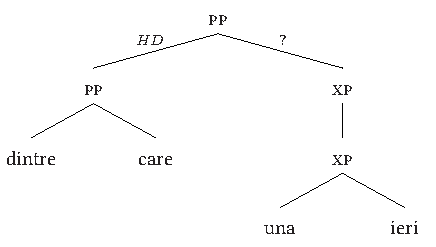
\includegraphics{figures/Ch3Fig6b.pdf} % \documentclass[12pt]{article}
\usepackage[latin1]{inputenc}
%\documentclass[twoside,14pt,a4paper]{article}
\usepackage{fullpage}
%\usepackage{times}
\usepackage{latexsym}
\usepackage{ecltree+}
\usepackage{avm}
\usepackage{avm+}
%\usepackage[utf8]{inputenc}
%\usepackage[francais]{babel}

\usepackage{combelow}

\usepackage{xyling}

\begin{document}


\noindent{\textbf{Figure 1 \hspace{1cm} Analyse par reconstruction syntaxique}}
\vspace{1mm}

\Tree[2]{         & \K{\textsc{s}}\B{dl}\B{dr}       & \\
              \K{dont} && \K{\textsc{s}}\B{dl}\B{d}     & \\
               & \K{\textsc{np}}\B{d} & \K{\textsc{vp}}\B{d}\B{dr}\B{drr} & &\\  
       & \K{Marie} & \K{$<$est$>$} & \K{$<$venue$>$} & \K{hier}}


\bigskip



\noindent{\textbf{Figure 2 \hspace{1cm} Analyse en termes de fragment}}
\vspace{1mm}

\Tree[2]{         & \K{\textsc{xp}}\B{dl}\B{dr} &\\  
               \K{dont} && \K{\textsc{xp}}\B{d}\\
       && \K{\textsc{xp}}\B{dl}\B{dr} &\\
      & \K{Marie} && \K{hier}}


\bigskip



\noindent{\textbf{Figure 3 \hspace{1cm} Hi\'erarchie de syntagmes en HPSG, incluant le fragment et le cluster}}
\noindent

\Tree[2] {&& \K[6.2]{\textit{phrase}}\Bkk{6.2,0}{0,0}{dl}\Bkk{6.2,0}{0,0}{drr}		\\
&\K{\textit{non-hd-ph}}\B{dl}\B{dr} &&& \K{\textit{hd-ph}}\B{dl}\B{dr}\B{drrr} \\ 
\K{\textbf{\textit{cluster-ph}}} & &  \K{\textit{coord-ph}} & \K{\textit{hd-only-ph}}\B{d} && \K{\textit{hd-adj-ph}} && \K{\textit{hd-nexus-ph}}\B{dll}\B{dl}\B{d}\B{dr}\\
& & & \K{\textbf{\textit{hd-fragm-ph}}} && \K{\textit{hd-comps}} & \K{\textit{hd-subj}} & \K{\textit{hd-filler}} & \K{\textit{...}}}


%\bigskip
\newpage



\noindent{\textbf{Figure 4 \hspace{1cm} Repr\'esentation simplifi\'ee d'un fragment contenant un cluster de deux constituants}}

\regAvmFonts\avmoptions{center}

\newcommand{\AVMXPone}{\begin{Avm}{XP}
        \[\tp{head-fragment-ph}\\ synsem & \@{2} \[head \@{1}\]\\ mrkg & nil \]
        \end{Avm} }
\newcommand{\AVMXPtwo}{\begin{Avm}{XP}
				\[\tp{cluster-ph} \\ synsem & \@{2} \[head \@{1} & \[cluster & \<\@{3}, \@{4} \> \] \] \] 
				\end{Avm}} 
\newcommand{\AVMNPone}{\begin{Avm}{NP}
    \[synsem & \@{3} \]
\end{Avm}}
\newcommand{\AVMNPtwo}{\begin{Avm}{NP}
    \[synsem & \@{4} \] 
    \end{Avm}}       
    

\smallAvmFonts
\begin{figure}[hbcd]
  \begin{center}
     \begin{bundle}{\AVMXPone}\setlength{\GapDepth}{40pt}
       \chunk[\textsc{hd}]{\setlength{\GapWidth}{45pt}
       		\begin{bundle}{\AVMXPtwo}
               \chunk[\textsc{n-hd}]{\setlength{\GapWidth}{70pt}\setlength{\GapDepth}{20pt}
                  \begin{bundle}{\AVMNPone}
                    \chunk{Marie}
                  \end{bundle}}
               \chunk[\textsc{n-hd}]{\setlength{\GapDepth}{20pt}
                  \begin{bundle}{\AVMNPtwo}
                    \chunk{hier}
                  \end{bundle}}
             \end{bundle}}
             
         \end{bundle}
       	      
    
  \end{center}
\end{figure}
\regAvmFonts


\newpage



\noindent{\textbf{Figure 5 \hspace{1cm} Repr\'esentation simplifi\'ee d'un fragment contenant un cluster unaire}}

\regAvmFonts\avmoptions{center}

\newcommand{\AVMXPthree}{\begin{Avm}{XP}
        \[\tp{head-fragment-ph}\\ synsem & \@{2} \[head \@{1}\]\\ mrkg & nil \]
        \end{Avm} }
\newcommand{\AVMXPfour}{\begin{Avm}{XP}
				\[\tp{cluster-ph} \\ synsem & \@{2} \[head \@{1} & \[cluster & \<\@{3}NP \> \] \] \] 
				\end{Avm}} 
\newcommand{\AVMNPthree}{\begin{Avm}{NP}
    \[synsem & \@{3} \]
\end{Avm}}
          

\smallAvmFonts
\begin{figure}[hbcd]
  \begin{center}
     \begin{bundle}{\AVMXPthree}\setlength{\GapDepth}{40pt}
       \chunk[\textsc{hd}]{\setlength{\GapWidth}{45pt}
       		\begin{bundle}{\AVMXPfour}
               \chunk[\textsc{n-hd}]{\setlength{\GapWidth}{70pt}\setlength{\GapDepth}{20pt}
                  \begin{bundle}{\AVMNPthree}
                    \chunk{Marie}
                  \end{bundle}}
               
             \end{bundle}}
             
         \end{bundle}
       	      
    
  \end{center}
\end{figure}
\regAvmFonts


\bigskip



\noindent{\textbf{Figure 6 \hspace{1cm} Relations fonctionnelles possibles dans la RSV}
\vspace{1mm}

\noindent
\Tree{ &&& \K{\textsc{xp}}\B{dll}_{?}\B{drr}^{HD}  &&&\\
          & \K{\textsc{pp}}\B{dl}\B{dr} & && & \K{\textsc{xp}}\B{d} &\\                         
\K{dintre} && \K{care} &&& \K{\textsc{xp}}\B{dl}\B{dr}\\
&&&&      \K{una} && \K{ieri}}

\paragraph{}

\Tree{&&& \K{\textsc{pp}}\B{dll}_{HD}\B{drr}^{?} &&&\\
          & \K{\textsc{pp}}\B{dl}\B{dr} & && & \K{\textsc{xp}}\B{d} &\\                         
\K{dintre} && \K{care} &&& \K{\textsc{xp}}\B{dl}\B{dr}\\
&&&&      \K{una} && \K{ieri}}

\paragraph{}

\Tree{&&& \K{\textsc{xp}}\B{dll}_{N-HD}\B{drr}^{N-HD} &&&\\
       & \K{\textsc{pp}}\B{dl}\B{dr} & && & \K{\textsc{xp}}\B{d} &\\                         
\K{dintre} && \K{care} &&& \K{\textsc{xp}}\B{dl}\B{dr}\\
&&&&      \K{una} && \K{ieri}}


\bigskip



\noindent{\textbf{Figure 7 \hspace{1cm} Le syntagme de type t\^ete-foncteur dans une hi\'erarchie de syntagmes}

\noindent
\Tree[2]{ & \K[5.2]{\textit{phrase}}\Bkk{5.2,0}{0,0}{dl}\Bkk{5.2,0}{0,0}{dr}		\\
\K{\textit{non-hd-ph}}	&			 & \K[5.2]{\textit{hd-ph}}\Bkk{5.2,0}{0,0}{dl}\Bkk{5.2,0}{0,0}{dr}\Bkk{5.2,0}{0,0}{drrrr}  \\
& \K{\textit{hd-only-ph}}\B{d} & &   \K{\textit{hd-adj-ph}}\B{d}\B{dr} &&& \K{\textit{hd-nexus-ph}}\B{dl}\B{dr}\B{drr}\\
& \K{\textit{hd-fragm-ph}} && \K{\textbf{\textit{hd-funct-ph}}} & \K{\textit{...}} & \K{\textit{hd-comps-ph}} && \K{\textit{hd-subj-ph}} & \K{\textit{...}}}


\bigskip



\noindent{\textbf{Figure 8 \hspace{1cm} Arbre avec un syntagme t\^ete-foncteur}}

\regAvmFonts\avmoptions{center}
\newcommand{\AVMXPfive}{\begin{Avm}{XP}
        \[\tp{head-functor-ph}\\ head & \@{1}\\ mrkg & \@{2} marked\]
      									\end{Avm}}
\newcommand{\AVMPPone}{\begin{Avm}{PP}
        \[cat & \[head & \[select & \@{3}\]\\ mrkg & \@{2}\]\]
      									\end{Avm}}
\newcommand{\AVMXPsix}{\begin{Avm}{XP}
  \@{3}\[cat & \[head & \@{1}\\ mrkg & unmarked\]\]
      									\end{Avm}}
\newcommand{\AVMXPsixbis}{\begin{Avm}{XP} 
        							 \end{Avm}}
\newcommand{\AVMNPfirst}{\begin{Avm}{NP} 
        							 \end{Avm}}


\smallAvmFonts
\begin{figure}[hbcd]
  \begin{center}\setlength{\GapWidth}{60pt}\setlength{\GapDepth}{30pt}
     \begin{bundle}{\AVMXPfive}     	  			
     \chunk[\textsc{fct}]{\setlength{\GapWidth}{60pt}\setlength{\GapDepth}{20pt}
         \begin{bundle}{\AVMPPone}
           \chunk{parmi}
           \chunk{lesquelles}
         \end{bundle}}
     
  		\chunk[\textsc{hd}]{\setlength{\GapWidth}{60pt}\setlength{\GapDepth}{15pt}
         \begin{bundle}{\AVMXPsix}
         	\chunk{\setlength{\GapDepth}{15pt}\begin{bundle}{\AVMXPsixbis}
         	 \chunk{\setlength{\GapDepth}{15pt}\begin{bundle}{\AVMNPfirst}
           \chunk{Marie}
           \end{bundle}}
           \end{bundle}}  
         \end{bundle}}
 
     \end{bundle}
         
  \end{center}
\end{figure}
\regAvmFonts


\newpage



\noindent{\textbf{Figure 9 \hspace{1cm} Syntaxe simplifi\'ee des constructions \`a RSV en fran\c{c}ais}}

\Tree{ &&& \K{\textsc{s}}\B{dll}_{HD}\B{drrr}^{ADJ}  &&\\
& \K{\textsc{s}}\B{dl}_{SUBJ}\B{dr}^{HD} & && && \K{\textsc{xp}}\B{dl}_{FCT}\B{drr}^{HD} &\\ 
\K{\textsc{np}}\TRi && \K{\textsc{v}}\B{d} &&& \K{\textsc{pp}}\B{dl}_{HD}\B{dr}^{COMPS} & && \K{\textsc{xp}}\B{d}^{HD} &\\
\K{plusieurs}\Below{personnes} && \K{chantent} && \K{\textsc{p}rep}\B{d} && \K{\textsc{np}}\TRi && \K{\textsc{xp}}\B{d}^{N-HD}\\
&&&& \K{parmi} && \K{lesquelles} && \K{\textsc{np}}\TRi\\
&&&& && & & \K{Marie}}


\bigskip



\noindent{\textbf{Figure 10 \hspace{1cm} Syntaxe simplifi\'ee des constructions \`a RSV en roumain}}

\Tree{ &&& \K{\textsc{s}}\B{dll}_{HD}\B{drrr}^{ADJ}  &&\\
& \K{\textsc{s}}\B{dl}_{HD}\B{dr}^{SUBJ} & && && \K{\textsc{xp}}\B{dl}_{FCT}\B{drr}^{HD} &\\ 
\K{\textsc{v}}\B{d} && \K{\textsc{np}}\TRi &&& \K{\textsc{pp}}\B{dl}_{HD}\B{dr}^{COMPS} & && \K{\textsc{xp}}\B{d}^{HD} &\\
\K{vin} && \K{mai}\Below{multe}\Below{persoane} && \K{\textsc{p}rep}\B{d} && \K{\textsc{np}}\TRi && \K{\textsc{xp}}\B{d}^{N-HD}\\
&&&& \K{printre} && \K{care} && \K{\textsc{np}}\TRi\\
&&&& && & & \K{\c{s}i Maria}}

  
\newpage



\noindent{\textbf{Figure 11 \hspace{1cm} Relation \`a distance entre l'introducteur et l'\'el\'ement distingu\'e: accessibilit\'e de l'\'el\'ement distingu\'e dans le corps de la RSV}}      									      				

\regAvmFonts\avmoptions{center}
\newcommand{\AVMXPseven}{\begin{Avm}{XP}
        \[\tp{head-functor-ph} \\ ss & \[ head & \@{6} noun \\ mrkg & \@{7} \\ rel & \{\@{4}\} \] \] 
        									\end{Avm}}
        									
\newcommand{\AVMPPtwo}{\begin{Avm}{PP}
        \[\tp{head-comps-ph} \\ ss & \[ head & \[select & \@{1}  \] \\ mrkg & \@{7}\\ rel & \{\@{4}\} \] \] 
        							 \end{Avm}}
        							 
\newcommand{\AVMPrepone}{\begin{Avm}{Prep}
  			\[cat & \[head & \[select & \@{1} \[cont & \[anchors & \<\[ind & \@{3}\]\>\]\]\] \\ mrkg & \@{7}\\ val & \[comps & \<\@{2}\>\] \\ arg-st & \<\@{1}, \@{2}\> \] \\
  			  cont & \[ltop & \@{5} \\ rels & \<\[\tp{sum-subpart-rel} \\ label & \@{5} \\ subpart & \@{3} \\ sum & \@{4} \] \> \] \]
      									\end{Avm}}
      									
\newcommand{\AVMNPfour}{\begin{Avm}{NP}
   \[ss &\@{2}\[cat & \[head & noun\]\\ cont & \[ind & \@{4}\] \\ rel & \{\@{4}\}\] \]
        							 \end{Avm}}

\newcommand{\AVMXPeight}{\begin{Avm}{XP}
   \[\tp{head-fragment-ph} \\ ss &\@{1}\[cat & \[head & \@{6} noun\]\\ cont & \[ind & \@{3}\] \]\] 
        							 \end{Avm}}
        							 
\newcommand{\AVMXPeightbis}{\begin{Avm}{XP} 
        							 \end{Avm}}
\newcommand{\AVMNPsecond}{\begin{Avm}{NP} 
        							 \end{Avm}}        							 

\smallAvmFonts
\begin{figure}[hbcd]
  \begin{center}\setlength{\GapWidth}{100pt}\setlength{\GapDepth}{30pt}
     \begin{bundle}{\AVMXPseven}     	  			
   		\chunk[\textsc{fct}]{\setlength{\GapWidth}{140pt}\setlength{\GapDepth}{20pt}
         \begin{bundle}{\AVMPPtwo}
         	 \chunk[\textsc{hd}]{
         	 	\begin{bundle}{\AVMPrepone}
           		\chunk{parmi}
         		 \end{bundle}}
         	  \chunk[\textsc{comps}]{
         	 	 \begin{bundle}{\AVMNPfour}
           	 	\chunk{lesquelles}
         		 \end{bundle}}
         	\end{bundle}}
       \chunk[\textsc{hd}]{\setlength{\GapDepth}{15pt}
         	 	 \begin{bundle}{\AVMXPeight}
           	 	\chunk{\setlength{\GapDepth}{15pt}\begin{bundle}{\AVMXPeightbis}
         	 \chunk{\setlength{\GapDepth}{15pt}\begin{bundle}{\AVMNPsecond}
           \chunk{Marie}
           \end{bundle}}
           \end{bundle}}
         		 \end{bundle}}
      \end{bundle}
         
  \end{center}
\end{figure}
\regAvmFonts


\newpage



\noindent{\textbf{Figure 12 \hspace{1cm} Relation \`a distance entre la RSV et son ant\'ec\'edent: accessibilit\'e de l'ant\'ec\'edent dans la phrase h\^ote}}

\regAvmFonts\avmoptions{center}
\newcommand{\AVMSone}{\begin{Avm}{S}
        \[\tp{head-functor-ph}\] 
       							 \end{Avm}}
        							 
\newcommand{\AVMStwo}{\begin{Avm}{S}
   \[ss & \@{2}\[cont & \[ind & \@{6} \\ rels & \@{9}\] \] \]
        							 \end{Avm}}
        							 
\newcommand{\AVMNPfive}{\begin{Avm}{NP$_i$}
    	 \[cont & \[ind & \@{4}\] \] 
        							 \end{Avm}}

\newcommand{\AVMVone}{\begin{Avm}{V} 
        							 \end{Avm}}
        							         							 
\newcommand{\AVMXPnine}{\begin{Avm}{XP}
        \[ss & \[cat & \[head & \@{1} \[select & \@{2}\[ cont \[ anchors & \<\[ind & \@{4}\]\>\]\]\] \\
         mrkg & \@{10} \] \\
         cont & \[ind & \@{7}\]\\
         c-cont & \[rels & \<\[\tp{sum-subpart-rel}\\ 
         											subpart & \@{7} event\\
         											sum & \@{6} event\]\>\] \\
											rel & \{\@{4}\}\] \]
        									\end{Avm}}
        									        							 
\newcommand{\AVMPPthree}{\begin{Avm}{PP}
  			 \[ss &\[cat & \[head & \[select & \@{3} \] \\
         mrkg & \@{10} \]\\
			cont & \[ltop & \@{5} \\ rels & \<\[\tp{sum-subpart-rel} \\ label & \@{5} \\ subpart & \@{8} \\ sum & \@{4} \] \> \] \\
			rel & \{\@{4}\}\] \]
      									\end{Avm}}
      									
\newcommand{\AVMXPten}{\begin{Avm}{XP}
   			\[ss &\@{3}\[cat \[head & \@{1}\] \\ 
			cont \[ind  \@{7}\\
   								anchors & \<\[ind & \@{8}\]\>\]\\
   				fragment \[source \[ind & \@{6} \\ rels & \@{9}\]\\
   										abstract-cont \@{B}\]\] \]
        							 \end{Avm}}

\newcommand{\AVMXPtenbis}{\begin{Avm}{XP} 
        							 \end{Avm}}
\newcommand{\AVMNPthird}{\begin{Avm}{NP} 
        							 \end{Avm}}

\smallAvmFonts
\begin{figure}[hbcd]
  \begin{center}\setlength{\GapDepth}{25pt}
     \begin{bundle}{\AVMSone}     	  			
   		\chunk[\textsc{hd}]{
         \begin{bundle}{\AVMStwo}
         	 \chunk[\textsc{subj}]{
         	 	\begin{bundle}{\AVMNPfive}
           		\chunk{plusieurs personnes}
         		 \end{bundle}}
    
         	  \chunk[\textsc{hd}]{
         	 	 \begin{bundle}{\AVMVone}
           	 	\chunk{chantent}
         		 \end{bundle}}
         		 \end{bundle}}
         	
     \chunk[\textsc{fct}]{\setlength{\GapWidth}{110pt}\setlength{\GapDepth}{30pt}
       \begin{bundle}{\AVMXPnine}
         	\chunk[\textsc{fct}]{\setlength{\GapWidth}{30pt}
         	 	\begin{bundle}{\AVMPPthree}
           		\chunk{parmi}
           		\chunk{lesquelles$_i$}
         		 \end{bundle}}
          \chunk[\textsc{hd}]{\setlength{\GapWidth}{20pt}\setlength{\GapDepth}{15pt}
         	 	\begin{bundle}{\AVMXPten}
           	 	\chunk{\setlength{\GapDepth}{15pt}\begin{bundle}{\AVMXPtenbis}
         	 \chunk{\setlength{\GapDepth}{15pt}\begin{bundle}{\AVMNPthird}
           \chunk{Marie}
           \end{bundle}}
           \end{bundle}}
         		 \end{bundle}}	 
         	 \end{bundle}}
         	 	
        \end{bundle}
         
  \end{center}
\end{figure}
\regAvmFonts


\newpage



\noindent{\textbf{Figure 13 \hspace{1cm} Arbre avec le compl\'ementeur \textit{dont} dans les relatives ordinaires}}

\regAvmFonts\avmoptions{center}

\newcommand{\AVMNPsix}{\begin{Avm}{NP}
        \[\tp{head-functor-ph}\]
      \end{Avm}}
\newcommand{\AVMNPseven}{\begin{avm} \@1NP$_i$
      \end{avm}}
\newcommand{\AVMSthree}{\begin{Avm}{S}
    \[head & \[select & \@{1} \] \\ mrkg & dont \\ slash & \{ \} \] 
    \end{Avm}}
\newcommand{\AVMCompr}{\begin{Avm}{Compr}
    \[head & \[vform & \@{2}\]\\ mrkg & dont \\ comps & \<\@{3}\>\\ bind & \{\@{4}\} \\ slash & \{\} \]
		\end{Avm}}
\newcommand{\AVMSfour}{\begin{Avm}{S}
\@{3}\[vform & \@{2} tensed \\ subj & \< \>\\ slash & \{\@{4}PP$_i$[\textit{de}] \}\\ mrkg & unmarked \]
\end{Avm}}
\newcommand{\AVMNPeight}{\begin{Avm}{NP}
    \end{Avm}}
\newcommand{\AVMVtwo}{\begin{Avm}{V}
		\[slash & \{\@{4}\}\]
    \end{Avm}}
    
\smallAvmFonts
\begin{figure}[hbcd]

\begin{center}\setlength{\GapWidth}{40pt}\setlength{\GapDepth}{20pt}
     \begin{bundle}{\AVMNPsix}
     
\chunk[\textsc{hd}]{\setlength{\GapDepth}{30pt}
			\begin{bundle}{\AVMNPseven}
               \chunk{l'histoire}
               \end{bundle}
         }

\chunk[\textsc{fct}]{\setlength{\GapWidth}{80pt}\setlength{\GapDepth}{20pt}
         \begin{bundle}{\AVMSthree}
           \chunk[\textsc{hd}]{
             \begin{bundle}{\AVMCompr}
             		\chunk{dont}
               		\end{bundle}
        			 }
             
               \chunk[\textsc{comps}]{
                  \begin{bundle}{\AVMSfour}
                    \chunk[\textsc{subj}]{
                      \begin{bundle}{\AVMNPeight}
                      \chunk{Marie}
               		\end{bundle}
        			 }
                  
               \chunk[\textsc{hd}]{
                  \begin{bundle}{\AVMVtwo}
                    \chunk{parle}
                  \end{bundle}}
             \end{bundle}
           }
         \end{bundle}
       }
     
     \end{bundle}
  \end{center}
\end{figure}
\regAvmFonts


\newpage



\noindent{\textbf{Figure 14 \hspace{1cm} Arbre avec l'introducteur \textit{dont} dans les RSV}}

\regAvmFonts\avmoptions{center}
\newcommand{\AVMSfive}{\begin{Avm}{S}
        \[\tp{head-functor-ph}\] 
       							 \end{Avm}}
        							 
\newcommand{\AVMSsix}{\begin{Avm}{S}
    \[\tp{head-subject-ph} \\ ss & \@{2}\[cont & \[ind & \@{6}\] \] \]
        							 \end{Avm}}
        							 
\newcommand{\AVMNPnine}{\begin{Avm}{NP}
    	 \[ss & \[cont & \[ind & \@{4}\] \] \] 
        							 \end{Avm}}

\newcommand{\AVMVthree}{\begin{Avm}{V} 
        							 \end{Avm}}
        							         							 
\newcommand{\AVMXPeleven}{\begin{Avm}{XP}
        \[\tp{head-functor-ph} \\ ss & \[cat & \[head \@{1} & \[select & \@{2} \] \\ mrkg & dont \] \] \]
        									\end{Avm}}
        									        							 
\newcommand{\AVMYPone}{\begin{Avm}{?P}
  			\[ss & \[cat & \[head & \[select & \[cat \[head \| select \@{7} \| cont \[anchors & \<\[ind & \@{4}\]\> \] \] \\ cont \[anchors & \<\[ind & \@{3}\]\> \] \] \] \\ mrkg & dont\] \\
  			cont & \[ltop & \@{5} \\ rels & \<\[\tp{sum-subpart-rel} \\ label & \@{5} \\ subpart & \@{3} \\ sum & \@{4} \] \> \] \] \]
      									\end{Avm}}
      									
\newcommand{\AVMXPtwelve}{\begin{Avm}{XP}
   \[\tp{head-fragment-phrase}\\ ss & \@{7}\[cat & \[head & \@{1}\] \\ cont & \[ind & \@{3}\]\] \]
        							 \end{Avm}}

\newcommand{\AVMXPtwelvebis}{\begin{Avm}{XP} 
        							 \end{Avm}}
\newcommand{\AVMNPfourth}{\begin{Avm}{NP} 
        							 \end{Avm}}

\smallAvmFonts
\begin{figure}[hbcd]
  \begin{center}\setlength{\GapWidth}{50pt}\setlength{\GapDepth}{25pt}
     \begin{bundle}{\AVMSfive}     	  			
   		\chunk[\textsc{hd}]{\setlength{\GapWidth}{10pt}
         \begin{bundle}{\AVMSsix}
         	 \chunk[\textsc{subj}]{\setlength{\GapDepth}{15pt}
         	 	\begin{bundle}{\AVMNPnine}
           		\chunk{plusieurs personnes}
         		 \end{bundle}}
    
         	  \chunk[\textsc{hd}]{\setlength{\GapDepth}{19pt}
         	 	 \begin{bundle}{\AVMVthree}
           	 	\chunk{chantent}
         		 \end{bundle}}
         		 \end{bundle}}
         	
     \chunk[\textsc{fct}]{\setlength{\GapWidth}{200pt}\setlength{\GapDepth}{80pt}
       \begin{bundle}{\AVMXPeleven}
         	\chunk[\textsc{fct}]{\setlength{\GapWidth}{100pt}\setlength{\GapDepth}{40pt}
         	 	\begin{bundle}{\AVMYPone}
           		\chunk{dont}
         		 \end{bundle}}
          		\chunk[\textsc{hd}]{\setlength{\GapWidth}{130pt}\setlength{\GapDepth}{15pt}
         	 	\begin{bundle}{\AVMXPtwelve}
           	 	\chunk{\setlength{\GapDepth}{15pt}
           	 	\begin{bundle}{\AVMXPtwelvebis}
         	 \chunk{\setlength{\GapDepth}{15pt}
         	 \begin{bundle}{\AVMNPfourth}
           \chunk{Marie}
           \end{bundle}}
           \end{bundle}}
         		 \end{bundle}}	 
         	 \end{bundle}}
         	 	
        \end{bundle}
         
  \end{center}
\end{figure}
\regAvmFonts


\end{document}
\caption{Analyse B : L’introducteur est la tête.}
\label{ch3:fig6b}
\end{figure}

\begin{figure}
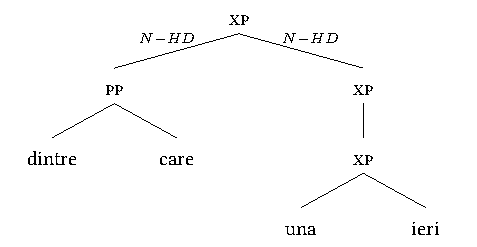
\includegraphics{figures/Ch3Fig6c.pdf} % \documentclass[12pt]{article}
\usepackage[latin1]{inputenc}
%\documentclass[twoside,14pt,a4paper]{article}
\usepackage{fullpage}
%\usepackage{times}
\usepackage{latexsym}
\usepackage{ecltree+}
\usepackage{avm}
\usepackage{avm+}
%\usepackage[utf8]{inputenc}
%\usepackage[francais]{babel}

\usepackage{combelow}

\usepackage{xyling}

\begin{document}


\noindent{\textbf{Figure 1 \hspace{1cm} Analyse par reconstruction syntaxique}}
\vspace{1mm}

\Tree[2]{         & \K{\textsc{s}}\B{dl}\B{dr}       & \\
              \K{dont} && \K{\textsc{s}}\B{dl}\B{d}     & \\
               & \K{\textsc{np}}\B{d} & \K{\textsc{vp}}\B{d}\B{dr}\B{drr} & &\\  
       & \K{Marie} & \K{$<$est$>$} & \K{$<$venue$>$} & \K{hier}}


\bigskip



\noindent{\textbf{Figure 2 \hspace{1cm} Analyse en termes de fragment}}
\vspace{1mm}

\Tree[2]{         & \K{\textsc{xp}}\B{dl}\B{dr} &\\  
               \K{dont} && \K{\textsc{xp}}\B{d}\\
       && \K{\textsc{xp}}\B{dl}\B{dr} &\\
      & \K{Marie} && \K{hier}}


\bigskip



\noindent{\textbf{Figure 3 \hspace{1cm} Hi\'erarchie de syntagmes en HPSG, incluant le fragment et le cluster}}
\noindent

\Tree[2] {&& \K[6.2]{\textit{phrase}}\Bkk{6.2,0}{0,0}{dl}\Bkk{6.2,0}{0,0}{drr}		\\
&\K{\textit{non-hd-ph}}\B{dl}\B{dr} &&& \K{\textit{hd-ph}}\B{dl}\B{dr}\B{drrr} \\ 
\K{\textbf{\textit{cluster-ph}}} & &  \K{\textit{coord-ph}} & \K{\textit{hd-only-ph}}\B{d} && \K{\textit{hd-adj-ph}} && \K{\textit{hd-nexus-ph}}\B{dll}\B{dl}\B{d}\B{dr}\\
& & & \K{\textbf{\textit{hd-fragm-ph}}} && \K{\textit{hd-comps}} & \K{\textit{hd-subj}} & \K{\textit{hd-filler}} & \K{\textit{...}}}


%\bigskip
\newpage



\noindent{\textbf{Figure 4 \hspace{1cm} Repr\'esentation simplifi\'ee d'un fragment contenant un cluster de deux constituants}}

\regAvmFonts\avmoptions{center}

\newcommand{\AVMXPone}{\begin{Avm}{XP}
        \[\tp{head-fragment-ph}\\ synsem & \@{2} \[head \@{1}\]\\ mrkg & nil \]
        \end{Avm} }
\newcommand{\AVMXPtwo}{\begin{Avm}{XP}
				\[\tp{cluster-ph} \\ synsem & \@{2} \[head \@{1} & \[cluster & \<\@{3}, \@{4} \> \] \] \] 
				\end{Avm}} 
\newcommand{\AVMNPone}{\begin{Avm}{NP}
    \[synsem & \@{3} \]
\end{Avm}}
\newcommand{\AVMNPtwo}{\begin{Avm}{NP}
    \[synsem & \@{4} \] 
    \end{Avm}}       
    

\smallAvmFonts
\begin{figure}[hbcd]
  \begin{center}
     \begin{bundle}{\AVMXPone}\setlength{\GapDepth}{40pt}
       \chunk[\textsc{hd}]{\setlength{\GapWidth}{45pt}
       		\begin{bundle}{\AVMXPtwo}
               \chunk[\textsc{n-hd}]{\setlength{\GapWidth}{70pt}\setlength{\GapDepth}{20pt}
                  \begin{bundle}{\AVMNPone}
                    \chunk{Marie}
                  \end{bundle}}
               \chunk[\textsc{n-hd}]{\setlength{\GapDepth}{20pt}
                  \begin{bundle}{\AVMNPtwo}
                    \chunk{hier}
                  \end{bundle}}
             \end{bundle}}
             
         \end{bundle}
       	      
    
  \end{center}
\end{figure}
\regAvmFonts


\newpage



\noindent{\textbf{Figure 5 \hspace{1cm} Repr\'esentation simplifi\'ee d'un fragment contenant un cluster unaire}}

\regAvmFonts\avmoptions{center}

\newcommand{\AVMXPthree}{\begin{Avm}{XP}
        \[\tp{head-fragment-ph}\\ synsem & \@{2} \[head \@{1}\]\\ mrkg & nil \]
        \end{Avm} }
\newcommand{\AVMXPfour}{\begin{Avm}{XP}
				\[\tp{cluster-ph} \\ synsem & \@{2} \[head \@{1} & \[cluster & \<\@{3}NP \> \] \] \] 
				\end{Avm}} 
\newcommand{\AVMNPthree}{\begin{Avm}{NP}
    \[synsem & \@{3} \]
\end{Avm}}
          

\smallAvmFonts
\begin{figure}[hbcd]
  \begin{center}
     \begin{bundle}{\AVMXPthree}\setlength{\GapDepth}{40pt}
       \chunk[\textsc{hd}]{\setlength{\GapWidth}{45pt}
       		\begin{bundle}{\AVMXPfour}
               \chunk[\textsc{n-hd}]{\setlength{\GapWidth}{70pt}\setlength{\GapDepth}{20pt}
                  \begin{bundle}{\AVMNPthree}
                    \chunk{Marie}
                  \end{bundle}}
               
             \end{bundle}}
             
         \end{bundle}
       	      
    
  \end{center}
\end{figure}
\regAvmFonts


\bigskip



\noindent{\textbf{Figure 6 \hspace{1cm} Relations fonctionnelles possibles dans la RSV}
\vspace{1mm}

\noindent
\Tree{ &&& \K{\textsc{xp}}\B{dll}_{?}\B{drr}^{HD}  &&&\\
          & \K{\textsc{pp}}\B{dl}\B{dr} & && & \K{\textsc{xp}}\B{d} &\\                         
\K{dintre} && \K{care} &&& \K{\textsc{xp}}\B{dl}\B{dr}\\
&&&&      \K{una} && \K{ieri}}

\paragraph{}

\Tree{&&& \K{\textsc{pp}}\B{dll}_{HD}\B{drr}^{?} &&&\\
          & \K{\textsc{pp}}\B{dl}\B{dr} & && & \K{\textsc{xp}}\B{d} &\\                         
\K{dintre} && \K{care} &&& \K{\textsc{xp}}\B{dl}\B{dr}\\
&&&&      \K{una} && \K{ieri}}

\paragraph{}

\Tree{&&& \K{\textsc{xp}}\B{dll}_{N-HD}\B{drr}^{N-HD} &&&\\
       & \K{\textsc{pp}}\B{dl}\B{dr} & && & \K{\textsc{xp}}\B{d} &\\                         
\K{dintre} && \K{care} &&& \K{\textsc{xp}}\B{dl}\B{dr}\\
&&&&      \K{una} && \K{ieri}}


\bigskip



\noindent{\textbf{Figure 7 \hspace{1cm} Le syntagme de type t\^ete-foncteur dans une hi\'erarchie de syntagmes}

\noindent
\Tree[2]{ & \K[5.2]{\textit{phrase}}\Bkk{5.2,0}{0,0}{dl}\Bkk{5.2,0}{0,0}{dr}		\\
\K{\textit{non-hd-ph}}	&			 & \K[5.2]{\textit{hd-ph}}\Bkk{5.2,0}{0,0}{dl}\Bkk{5.2,0}{0,0}{dr}\Bkk{5.2,0}{0,0}{drrrr}  \\
& \K{\textit{hd-only-ph}}\B{d} & &   \K{\textit{hd-adj-ph}}\B{d}\B{dr} &&& \K{\textit{hd-nexus-ph}}\B{dl}\B{dr}\B{drr}\\
& \K{\textit{hd-fragm-ph}} && \K{\textbf{\textit{hd-funct-ph}}} & \K{\textit{...}} & \K{\textit{hd-comps-ph}} && \K{\textit{hd-subj-ph}} & \K{\textit{...}}}


\bigskip



\noindent{\textbf{Figure 8 \hspace{1cm} Arbre avec un syntagme t\^ete-foncteur}}

\regAvmFonts\avmoptions{center}
\newcommand{\AVMXPfive}{\begin{Avm}{XP}
        \[\tp{head-functor-ph}\\ head & \@{1}\\ mrkg & \@{2} marked\]
      									\end{Avm}}
\newcommand{\AVMPPone}{\begin{Avm}{PP}
        \[cat & \[head & \[select & \@{3}\]\\ mrkg & \@{2}\]\]
      									\end{Avm}}
\newcommand{\AVMXPsix}{\begin{Avm}{XP}
  \@{3}\[cat & \[head & \@{1}\\ mrkg & unmarked\]\]
      									\end{Avm}}
\newcommand{\AVMXPsixbis}{\begin{Avm}{XP} 
        							 \end{Avm}}
\newcommand{\AVMNPfirst}{\begin{Avm}{NP} 
        							 \end{Avm}}


\smallAvmFonts
\begin{figure}[hbcd]
  \begin{center}\setlength{\GapWidth}{60pt}\setlength{\GapDepth}{30pt}
     \begin{bundle}{\AVMXPfive}     	  			
     \chunk[\textsc{fct}]{\setlength{\GapWidth}{60pt}\setlength{\GapDepth}{20pt}
         \begin{bundle}{\AVMPPone}
           \chunk{parmi}
           \chunk{lesquelles}
         \end{bundle}}
     
  		\chunk[\textsc{hd}]{\setlength{\GapWidth}{60pt}\setlength{\GapDepth}{15pt}
         \begin{bundle}{\AVMXPsix}
         	\chunk{\setlength{\GapDepth}{15pt}\begin{bundle}{\AVMXPsixbis}
         	 \chunk{\setlength{\GapDepth}{15pt}\begin{bundle}{\AVMNPfirst}
           \chunk{Marie}
           \end{bundle}}
           \end{bundle}}  
         \end{bundle}}
 
     \end{bundle}
         
  \end{center}
\end{figure}
\regAvmFonts


\newpage



\noindent{\textbf{Figure 9 \hspace{1cm} Syntaxe simplifi\'ee des constructions \`a RSV en fran\c{c}ais}}

\Tree{ &&& \K{\textsc{s}}\B{dll}_{HD}\B{drrr}^{ADJ}  &&\\
& \K{\textsc{s}}\B{dl}_{SUBJ}\B{dr}^{HD} & && && \K{\textsc{xp}}\B{dl}_{FCT}\B{drr}^{HD} &\\ 
\K{\textsc{np}}\TRi && \K{\textsc{v}}\B{d} &&& \K{\textsc{pp}}\B{dl}_{HD}\B{dr}^{COMPS} & && \K{\textsc{xp}}\B{d}^{HD} &\\
\K{plusieurs}\Below{personnes} && \K{chantent} && \K{\textsc{p}rep}\B{d} && \K{\textsc{np}}\TRi && \K{\textsc{xp}}\B{d}^{N-HD}\\
&&&& \K{parmi} && \K{lesquelles} && \K{\textsc{np}}\TRi\\
&&&& && & & \K{Marie}}


\bigskip



\noindent{\textbf{Figure 10 \hspace{1cm} Syntaxe simplifi\'ee des constructions \`a RSV en roumain}}

\Tree{ &&& \K{\textsc{s}}\B{dll}_{HD}\B{drrr}^{ADJ}  &&\\
& \K{\textsc{s}}\B{dl}_{HD}\B{dr}^{SUBJ} & && && \K{\textsc{xp}}\B{dl}_{FCT}\B{drr}^{HD} &\\ 
\K{\textsc{v}}\B{d} && \K{\textsc{np}}\TRi &&& \K{\textsc{pp}}\B{dl}_{HD}\B{dr}^{COMPS} & && \K{\textsc{xp}}\B{d}^{HD} &\\
\K{vin} && \K{mai}\Below{multe}\Below{persoane} && \K{\textsc{p}rep}\B{d} && \K{\textsc{np}}\TRi && \K{\textsc{xp}}\B{d}^{N-HD}\\
&&&& \K{printre} && \K{care} && \K{\textsc{np}}\TRi\\
&&&& && & & \K{\c{s}i Maria}}

  
\newpage



\noindent{\textbf{Figure 11 \hspace{1cm} Relation \`a distance entre l'introducteur et l'\'el\'ement distingu\'e: accessibilit\'e de l'\'el\'ement distingu\'e dans le corps de la RSV}}      									      				

\regAvmFonts\avmoptions{center}
\newcommand{\AVMXPseven}{\begin{Avm}{XP}
        \[\tp{head-functor-ph} \\ ss & \[ head & \@{6} noun \\ mrkg & \@{7} \\ rel & \{\@{4}\} \] \] 
        									\end{Avm}}
        									
\newcommand{\AVMPPtwo}{\begin{Avm}{PP}
        \[\tp{head-comps-ph} \\ ss & \[ head & \[select & \@{1}  \] \\ mrkg & \@{7}\\ rel & \{\@{4}\} \] \] 
        							 \end{Avm}}
        							 
\newcommand{\AVMPrepone}{\begin{Avm}{Prep}
  			\[cat & \[head & \[select & \@{1} \[cont & \[anchors & \<\[ind & \@{3}\]\>\]\]\] \\ mrkg & \@{7}\\ val & \[comps & \<\@{2}\>\] \\ arg-st & \<\@{1}, \@{2}\> \] \\
  			  cont & \[ltop & \@{5} \\ rels & \<\[\tp{sum-subpart-rel} \\ label & \@{5} \\ subpart & \@{3} \\ sum & \@{4} \] \> \] \]
      									\end{Avm}}
      									
\newcommand{\AVMNPfour}{\begin{Avm}{NP}
   \[ss &\@{2}\[cat & \[head & noun\]\\ cont & \[ind & \@{4}\] \\ rel & \{\@{4}\}\] \]
        							 \end{Avm}}

\newcommand{\AVMXPeight}{\begin{Avm}{XP}
   \[\tp{head-fragment-ph} \\ ss &\@{1}\[cat & \[head & \@{6} noun\]\\ cont & \[ind & \@{3}\] \]\] 
        							 \end{Avm}}
        							 
\newcommand{\AVMXPeightbis}{\begin{Avm}{XP} 
        							 \end{Avm}}
\newcommand{\AVMNPsecond}{\begin{Avm}{NP} 
        							 \end{Avm}}        							 

\smallAvmFonts
\begin{figure}[hbcd]
  \begin{center}\setlength{\GapWidth}{100pt}\setlength{\GapDepth}{30pt}
     \begin{bundle}{\AVMXPseven}     	  			
   		\chunk[\textsc{fct}]{\setlength{\GapWidth}{140pt}\setlength{\GapDepth}{20pt}
         \begin{bundle}{\AVMPPtwo}
         	 \chunk[\textsc{hd}]{
         	 	\begin{bundle}{\AVMPrepone}
           		\chunk{parmi}
         		 \end{bundle}}
         	  \chunk[\textsc{comps}]{
         	 	 \begin{bundle}{\AVMNPfour}
           	 	\chunk{lesquelles}
         		 \end{bundle}}
         	\end{bundle}}
       \chunk[\textsc{hd}]{\setlength{\GapDepth}{15pt}
         	 	 \begin{bundle}{\AVMXPeight}
           	 	\chunk{\setlength{\GapDepth}{15pt}\begin{bundle}{\AVMXPeightbis}
         	 \chunk{\setlength{\GapDepth}{15pt}\begin{bundle}{\AVMNPsecond}
           \chunk{Marie}
           \end{bundle}}
           \end{bundle}}
         		 \end{bundle}}
      \end{bundle}
         
  \end{center}
\end{figure}
\regAvmFonts


\newpage



\noindent{\textbf{Figure 12 \hspace{1cm} Relation \`a distance entre la RSV et son ant\'ec\'edent: accessibilit\'e de l'ant\'ec\'edent dans la phrase h\^ote}}

\regAvmFonts\avmoptions{center}
\newcommand{\AVMSone}{\begin{Avm}{S}
        \[\tp{head-functor-ph}\] 
       							 \end{Avm}}
        							 
\newcommand{\AVMStwo}{\begin{Avm}{S}
   \[ss & \@{2}\[cont & \[ind & \@{6} \\ rels & \@{9}\] \] \]
        							 \end{Avm}}
        							 
\newcommand{\AVMNPfive}{\begin{Avm}{NP$_i$}
    	 \[cont & \[ind & \@{4}\] \] 
        							 \end{Avm}}

\newcommand{\AVMVone}{\begin{Avm}{V} 
        							 \end{Avm}}
        							         							 
\newcommand{\AVMXPnine}{\begin{Avm}{XP}
        \[ss & \[cat & \[head & \@{1} \[select & \@{2}\[ cont \[ anchors & \<\[ind & \@{4}\]\>\]\]\] \\
         mrkg & \@{10} \] \\
         cont & \[ind & \@{7}\]\\
         c-cont & \[rels & \<\[\tp{sum-subpart-rel}\\ 
         											subpart & \@{7} event\\
         											sum & \@{6} event\]\>\] \\
											rel & \{\@{4}\}\] \]
        									\end{Avm}}
        									        							 
\newcommand{\AVMPPthree}{\begin{Avm}{PP}
  			 \[ss &\[cat & \[head & \[select & \@{3} \] \\
         mrkg & \@{10} \]\\
			cont & \[ltop & \@{5} \\ rels & \<\[\tp{sum-subpart-rel} \\ label & \@{5} \\ subpart & \@{8} \\ sum & \@{4} \] \> \] \\
			rel & \{\@{4}\}\] \]
      									\end{Avm}}
      									
\newcommand{\AVMXPten}{\begin{Avm}{XP}
   			\[ss &\@{3}\[cat \[head & \@{1}\] \\ 
			cont \[ind  \@{7}\\
   								anchors & \<\[ind & \@{8}\]\>\]\\
   				fragment \[source \[ind & \@{6} \\ rels & \@{9}\]\\
   										abstract-cont \@{B}\]\] \]
        							 \end{Avm}}

\newcommand{\AVMXPtenbis}{\begin{Avm}{XP} 
        							 \end{Avm}}
\newcommand{\AVMNPthird}{\begin{Avm}{NP} 
        							 \end{Avm}}

\smallAvmFonts
\begin{figure}[hbcd]
  \begin{center}\setlength{\GapDepth}{25pt}
     \begin{bundle}{\AVMSone}     	  			
   		\chunk[\textsc{hd}]{
         \begin{bundle}{\AVMStwo}
         	 \chunk[\textsc{subj}]{
         	 	\begin{bundle}{\AVMNPfive}
           		\chunk{plusieurs personnes}
         		 \end{bundle}}
    
         	  \chunk[\textsc{hd}]{
         	 	 \begin{bundle}{\AVMVone}
           	 	\chunk{chantent}
         		 \end{bundle}}
         		 \end{bundle}}
         	
     \chunk[\textsc{fct}]{\setlength{\GapWidth}{110pt}\setlength{\GapDepth}{30pt}
       \begin{bundle}{\AVMXPnine}
         	\chunk[\textsc{fct}]{\setlength{\GapWidth}{30pt}
         	 	\begin{bundle}{\AVMPPthree}
           		\chunk{parmi}
           		\chunk{lesquelles$_i$}
         		 \end{bundle}}
          \chunk[\textsc{hd}]{\setlength{\GapWidth}{20pt}\setlength{\GapDepth}{15pt}
         	 	\begin{bundle}{\AVMXPten}
           	 	\chunk{\setlength{\GapDepth}{15pt}\begin{bundle}{\AVMXPtenbis}
         	 \chunk{\setlength{\GapDepth}{15pt}\begin{bundle}{\AVMNPthird}
           \chunk{Marie}
           \end{bundle}}
           \end{bundle}}
         		 \end{bundle}}	 
         	 \end{bundle}}
         	 	
        \end{bundle}
         
  \end{center}
\end{figure}
\regAvmFonts


\newpage



\noindent{\textbf{Figure 13 \hspace{1cm} Arbre avec le compl\'ementeur \textit{dont} dans les relatives ordinaires}}

\regAvmFonts\avmoptions{center}

\newcommand{\AVMNPsix}{\begin{Avm}{NP}
        \[\tp{head-functor-ph}\]
      \end{Avm}}
\newcommand{\AVMNPseven}{\begin{avm} \@1NP$_i$
      \end{avm}}
\newcommand{\AVMSthree}{\begin{Avm}{S}
    \[head & \[select & \@{1} \] \\ mrkg & dont \\ slash & \{ \} \] 
    \end{Avm}}
\newcommand{\AVMCompr}{\begin{Avm}{Compr}
    \[head & \[vform & \@{2}\]\\ mrkg & dont \\ comps & \<\@{3}\>\\ bind & \{\@{4}\} \\ slash & \{\} \]
		\end{Avm}}
\newcommand{\AVMSfour}{\begin{Avm}{S}
\@{3}\[vform & \@{2} tensed \\ subj & \< \>\\ slash & \{\@{4}PP$_i$[\textit{de}] \}\\ mrkg & unmarked \]
\end{Avm}}
\newcommand{\AVMNPeight}{\begin{Avm}{NP}
    \end{Avm}}
\newcommand{\AVMVtwo}{\begin{Avm}{V}
		\[slash & \{\@{4}\}\]
    \end{Avm}}
    
\smallAvmFonts
\begin{figure}[hbcd]

\begin{center}\setlength{\GapWidth}{40pt}\setlength{\GapDepth}{20pt}
     \begin{bundle}{\AVMNPsix}
     
\chunk[\textsc{hd}]{\setlength{\GapDepth}{30pt}
			\begin{bundle}{\AVMNPseven}
               \chunk{l'histoire}
               \end{bundle}
         }

\chunk[\textsc{fct}]{\setlength{\GapWidth}{80pt}\setlength{\GapDepth}{20pt}
         \begin{bundle}{\AVMSthree}
           \chunk[\textsc{hd}]{
             \begin{bundle}{\AVMCompr}
             		\chunk{dont}
               		\end{bundle}
        			 }
             
               \chunk[\textsc{comps}]{
                  \begin{bundle}{\AVMSfour}
                    \chunk[\textsc{subj}]{
                      \begin{bundle}{\AVMNPeight}
                      \chunk{Marie}
               		\end{bundle}
        			 }
                  
               \chunk[\textsc{hd}]{
                  \begin{bundle}{\AVMVtwo}
                    \chunk{parle}
                  \end{bundle}}
             \end{bundle}
           }
         \end{bundle}
       }
     
     \end{bundle}
  \end{center}
\end{figure}
\regAvmFonts


\newpage



\noindent{\textbf{Figure 14 \hspace{1cm} Arbre avec l'introducteur \textit{dont} dans les RSV}}

\regAvmFonts\avmoptions{center}
\newcommand{\AVMSfive}{\begin{Avm}{S}
        \[\tp{head-functor-ph}\] 
       							 \end{Avm}}
        							 
\newcommand{\AVMSsix}{\begin{Avm}{S}
    \[\tp{head-subject-ph} \\ ss & \@{2}\[cont & \[ind & \@{6}\] \] \]
        							 \end{Avm}}
        							 
\newcommand{\AVMNPnine}{\begin{Avm}{NP}
    	 \[ss & \[cont & \[ind & \@{4}\] \] \] 
        							 \end{Avm}}

\newcommand{\AVMVthree}{\begin{Avm}{V} 
        							 \end{Avm}}
        							         							 
\newcommand{\AVMXPeleven}{\begin{Avm}{XP}
        \[\tp{head-functor-ph} \\ ss & \[cat & \[head \@{1} & \[select & \@{2} \] \\ mrkg & dont \] \] \]
        									\end{Avm}}
        									        							 
\newcommand{\AVMYPone}{\begin{Avm}{?P}
  			\[ss & \[cat & \[head & \[select & \[cat \[head \| select \@{7} \| cont \[anchors & \<\[ind & \@{4}\]\> \] \] \\ cont \[anchors & \<\[ind & \@{3}\]\> \] \] \] \\ mrkg & dont\] \\
  			cont & \[ltop & \@{5} \\ rels & \<\[\tp{sum-subpart-rel} \\ label & \@{5} \\ subpart & \@{3} \\ sum & \@{4} \] \> \] \] \]
      									\end{Avm}}
      									
\newcommand{\AVMXPtwelve}{\begin{Avm}{XP}
   \[\tp{head-fragment-phrase}\\ ss & \@{7}\[cat & \[head & \@{1}\] \\ cont & \[ind & \@{3}\]\] \]
        							 \end{Avm}}

\newcommand{\AVMXPtwelvebis}{\begin{Avm}{XP} 
        							 \end{Avm}}
\newcommand{\AVMNPfourth}{\begin{Avm}{NP} 
        							 \end{Avm}}

\smallAvmFonts
\begin{figure}[hbcd]
  \begin{center}\setlength{\GapWidth}{50pt}\setlength{\GapDepth}{25pt}
     \begin{bundle}{\AVMSfive}     	  			
   		\chunk[\textsc{hd}]{\setlength{\GapWidth}{10pt}
         \begin{bundle}{\AVMSsix}
         	 \chunk[\textsc{subj}]{\setlength{\GapDepth}{15pt}
         	 	\begin{bundle}{\AVMNPnine}
           		\chunk{plusieurs personnes}
         		 \end{bundle}}
    
         	  \chunk[\textsc{hd}]{\setlength{\GapDepth}{19pt}
         	 	 \begin{bundle}{\AVMVthree}
           	 	\chunk{chantent}
         		 \end{bundle}}
         		 \end{bundle}}
         	
     \chunk[\textsc{fct}]{\setlength{\GapWidth}{200pt}\setlength{\GapDepth}{80pt}
       \begin{bundle}{\AVMXPeleven}
         	\chunk[\textsc{fct}]{\setlength{\GapWidth}{100pt}\setlength{\GapDepth}{40pt}
         	 	\begin{bundle}{\AVMYPone}
           		\chunk{dont}
         		 \end{bundle}}
          		\chunk[\textsc{hd}]{\setlength{\GapWidth}{130pt}\setlength{\GapDepth}{15pt}
         	 	\begin{bundle}{\AVMXPtwelve}
           	 	\chunk{\setlength{\GapDepth}{15pt}
           	 	\begin{bundle}{\AVMXPtwelvebis}
         	 \chunk{\setlength{\GapDepth}{15pt}
         	 \begin{bundle}{\AVMNPfourth}
           \chunk{Marie}
           \end{bundle}}
           \end{bundle}}
         		 \end{bundle}}	 
         	 \end{bundle}}
         	 	
        \end{bundle}
         
  \end{center}
\end{figure}
\regAvmFonts


\end{document}
\caption{Analyse C : Il n’y a pas de tête.}
\label{ch3:fig6c}
\end{figure}


\subsubsection{Le corps de la RSV comme tête}\label{ch3:sect3.5.3.1}

L’argument le plus convaincant pour attribuer la fonction de tête au corps de la RSV est son emploi indépendant dans certains exemples. Les syntagmes constituant le corps de la RSV peuvent fonctionner de la même manière qu’une RSV dans son ensemble, en l’absence d’un introducteur. Ils se comportent comme des \is{ajout incident}ajouts incidents, avec une sémantique et une distribution similaires à celles qu’on observe dans les RSV. Ainsi, on trouve des \is{ajout incident}ajouts incidents sans introducteur, avec les deux types d’interprétations : une \isi{interprétation exemplifiante}, facilitée par la présence de l’adverbial \textit{în special} ‘notamment’ en roumain \REF{ch3:ex125a} ou \textit{notamment} en français \REF{ch3:ex126a}, ou encore une \isi{interprétation partitionnante} apparaissant surtout dans une structure coordonnée comme en \REF{ch3:ex125b} et (\ref{ch3:ex126b}--\ref{ch3:ex126c}).

\ea \label{ch3:ex125}
\ea 
Ţările din Europa de Est, [(\textbf{printre} \textbf{care}) în special România], reprezintă pieţele preferate de către mafioţii italieni pentru spălarea banilor. \label{ch3:ex125a}\\
\glt ‘Les pays de l’Europe de l’Est, (dont) notamment la Roumanie, représentent les marchés préférés par la mafia italienne pour le blanchiment  d’argent.’
\ex 
6~000 de zboruri au fost anulate, [(\textbf{dintre} \textbf{care}) aproape 70 doar în Bucureşti]. \label{ch3:ex125b}\\
\glt ‘6~000 vols ont été annulés, (dont) presque 70 seulement à Bucarest.’
\ex 
Şase persoane, [(\textbf{dintre} \textbf{care}) două din Gorj \uline{şi} patru din Mehedinţi], ar avea legături cu gruparea infracţională din care face parte şi Emilian Ştefan. \label{ch3:125c}\\
\glt ‘Six personnes, (dont) deux de Gorj et quatre de Mehedinţi, auraient des relations avec le groupe infractionnel dont Emilian Ştefan fait partie.’
\z 
\z

\ea \label{ch3:ex126} 
\ea 
De nombreuses espèces animales, [(\textbf{dont}) notamment les oursins], ont souffert de la pollution. \label{ch3:ex126a} 
\ex
Plusieurs personnes, [(\textbf{dont}) une hier \uline{et} deux ce matin], se sont plaintes de l’organisation. \label{ch3:ex126b}
\ex 
Plusieurs personnes, [(\textbf{dont}) Marie hier \uline{et} Jean ce matin], ont signalé le problème. \label{ch3:ex126c}
\z 
\z 

Par conséquent, la présence de l’introducteur n’est pas toujours nécessaire dans les syntagmes «~fragmentaires~» pour qu’ils fonctionnent comme ajouts avec une \isi{interprétation exemplifiante} ou \is{interprétation partitionnante}partitionnante. Il faut noter toutefois qu’en l’absence d’un introducteur, la sémantique de l’ajout n’est pas restreinte aux deux types d’interprétations mentionnées. Ainsi, les ajouts sans introducteur peuvent contenir un \isi{quantifieur universel} ou \is{quantifieur négatif}négatif (\ref{ch3:ex127}-\ref{ch3:ex128}), ce qui ne semble pas être le cas des RSV standard, comme le montrent les exemples (\ref{ch3:ex58}--\ref{ch3:ex59}) de la section~\ref{ch3:sect3.3.2.1}\footnote{Les ajouts qui sont compatibles avec un \isi{quantifieur universel} ou \is{quantifieur négatif}négatif permettent aussi l’emploi d’une conjonction (comme \textit{mais}), bien que l’introducteur \textit{dont} soit impossible.
\ea
\ea 
La secrétaire du labo a commandé plusieurs livres, [\{mais {\textbar} *dont\} \uline{tous} en anglais]. 
\ex 
La secrétaire du labo a commandé plusieurs livres, [\{mais {\textbar} *dont\} \uline{aucun} en français].
\z
\z
}.


\ea \label{ch3:ex127} 
\ea 
Am scris trei cărţi, [\uline{toate} pe aceeaşi temă]. \label{ch3:ex127a}\\
\glt ‘J’ai écrit trois livres, tous sur le même thème.’ 
\ex 
Patru fete, [\uline{niciuna} trecută de 23 ani], au decedat vineri seara în urma unui accident de circulaţie. \label{ch3:ex127b}\\
\glt ‘Quatre jeunes filles, aucune de plus de 23 ans, sont décédées vendredi soir à la suite d’un accident de la route.’
\z 
\z

\ea \label{ch3:ex128}
\ea 
Plusieurs livres, [\uline{tous} sur le même thème], ont été commandés. \label{ch3:ex128a} 
\ex
\%Quatre filles, [\uline{aucune} de plus de 23 ans], habitent dans cet immeuble délabré. \label{ch3:ex128b}
\z 
\z

Un argument contre l’analyse de l’introducteur comme tête concerne la réalisation syntaxique des arguments sémantiques de la tête de l’introducteur. A part la forme \textit{dont} en français, dont la catégorie est sujette à discussion, l’introducteur est toujours un syntagme prépositionnel (roum. \{\textit{printre / între / dintre}\} \textit{care} ou fr. \textit{parmi lesquel(le)s}). Une préposition, comme la forme \textit{printre} ‘parmi’ en roumain, introduit une relation sémantique entre deux arguments (indépendamment de son emploi dans les RSV ou en dehors des RSV) : l’un des arguments (noté \textit{Arg1} dans les exemples en \REF{ch3:ex129} est typiquement réalisé comme complément de la préposition, alors que l’autre (noté \textit{Arg2}) n’est pas réalisé dans le syntagme prépositionnel lui-même ({\cad} il est un argument externe). Ce deuxième argument n’est pas sélectionné par la préposition elle-même, mais plutôt par le syntagme prépositionnel dans son ensemble. Dans le cas des RSV, cet argument externe de la préposition n’est pas identifié avec l’antécédent de la RSV, mais plutôt avec l’élément distingué se trouvant dans le corps de la RSV. Il est donc légitime de considérer que les propriétés de sélection de l’introducteur et celles de la RSV dans son ensemble sont distinctes et, par conséquent, on ne doit pas analyser l’introducteur comme tête.  


\ea \label{ch3:ex129}
 
\ea
\gll Avem  [\ulg{un}{11}  spion]\textsubscript{Arg2}  [\textbf{printre}  [\uline{noi}]\textsubscript{Arg1}]. \label{ch3:ex129a}\\
avoir.\textsc{prs.1pl}  un  espion  parmi  nous \\
\glt ‘Nous avons un espion parmi nous.’

\ex 
\gll ... mai  multe  persoane,  [\textbf{printre}  [\uline{care}]\textsubscript{Arg1}]  [\uline{şi} \uline{Maria}]\textsubscript{Arg2}. \label{ch3:ex129b}\\
 ... plus  beaucoup.\textsc{adj}  personnes  parmi  lesquelles  aussi  Maria\\
\glt ‘... plusieurs personnes, parmi lesquelles Maria.’
\z 
\z


\subsubsection{L’introducteur de la RSV comme foncteur}\label{ch3:sect3.5.3.2}

L’introducteur de la RSV impose certaines contraintes : (i) il doit précéder le corps de la RSV (contrairement à des ajouts adverbiaux comme \textit{notamment} en (\ref{ch3:ex10}--\ref{ch3:ex11}) ci-dessus) ; (ii) il présente des propriétés de sélection ; (iii) au moins dans certains cas, il modifie la distribution du syntagme avec lequel il se combine.

Les relations fonctionnelles qui s’établissent entre l’introducteur et le corps d’une RSV rappellent les discussions portées autour de la relation fonctionnelle entre le déterminant et le nom à l’intérieur d’un groupe nominal. Ainsi, \citet{VanEynde2003,VanEynde2006,VanEynde2007} argumente en faveur d’une distinction qui doit être faite entre la notion de tête et la notion de sélecteur. En particulier, il considère que les prénominaux (déterminants, numéraux, etc.) de \il{italien}l’italien et du \ili{néerlandais} doivent être analysés comme des sélecteurs qui prennent un nominal comme leur tête et non comme leur complément (par exemple, dans le syntagme \textit{whose house}, le pronom au génitif \textit{whose} sélectionne un nom commun comme tête ; le syntagme dans son ensemble reçoit le cas de la tête nominale, cf. \is{Principe des traits de tête généralisé}le Principe des Traits de Tête, indépendamment du cas du pronom au génitif). Cette approche a l’avantage de rendre compte de manière satisfaisante des faits \is{accord}d’accord morpho-syntaxique dans un syntagme nominal (ou encore de l’accord sémantique dans une coordination nominale).

Par conséquent, Van Eynde introduit une nouvelle fonction syntaxique \textit{foncteur} (qui regroupe les fonctions de spécifieur, marqueur ou ajout pré-tête). Les foncteurs ne sont pas sous-catégorisés, au contraire ils sélectionnent une tête, à laquelle ils peuvent imposer un certain marquage. Une tête combinée avec un foncteur peut ainsi avoir une distribution différente de celle qu’elle pourrait avoir en emploi indépendant. 

\largerpage
On propose donc d’analyser l’introducteur de la RSV comme un foncteur\footnote{Le fait que l’introducteur de la RSV ne se comporte pas comme une tête ordinaire ou encore comme un ajout pourrait être pris en compte par des approches alternatives : l’introducteur de la RSV pourrait être analysé soit comme une \is{tête faible}tête «~faible~» (voir, dans ce sens, l’analyse proposée pour les conjonctions dans la section~\ref{ch2:sect2.5.2}), soit comme un marqueur. A priori, le choix d’une ou l’autre analyse ne fait pas de différence empirique majeure.}, sans pour autant étendre cette fonction aux constituants prénominaux\footnote{Bien que les arguments de Van Eynde soient convaincants, on reprend son analyse uniquement pour les introducteurs dans les RSV. Il reste à vérifier si on peut l’étendre aux prénominaux en roumain (et en français) ou encore à d’autres catégories comme les conjonctions ou les complémenteurs. Pour l’instant, on ne remet pas en cause ici la distinction entre spécifieurs et modifieurs.}. La \isi{linéarisation} stricte de l’introducteur par rapport au corps de la RSV, qui ne caractérise pas les ajouts, est un argument en faveur de cette analyse, cf. les exemples repris ci-dessous en (\ref{ch3:ex130}--\ref{ch3:ex131}).

\ea \label{ch3:ex130}
\ea
\gll Mai  multe  ţări  sud-americane,  [\textbf{printre} \textbf{care} şi  Brazilia], exportă  cafea  în  Europa. \\
plus  beaucoup.\textsc{adj}  pays  sud-américains  parmi  lesquels  aussi  Brésil.\textsc{def} 
exportent  café  en  Europe.\textsc{def} \\
\glt ‘Plusieurs pays sud-américains, parmi lesquels le Brésil, exportent du café vers l'Europe.’
\ex 
\gll *Mai  multe  ţări  sud-americane,  [şi  Brazilia  \textbf{printre} \textbf{care}], exportă  cafea  în  Europa.\\
plus  beaucoup.\textsc{adj}  pays  sud-américains  aussi  Brésil.\textsc{def}  parmi  lesquels exportent  café  en  Europe.\textsc{def} \\
\ex 
\gll Mai  multe  ţări,  [\textbf{printre} \textbf{care} în  mod  special Brazilia], exportă  cafea  în  Europa. \\
plus  beaucoup.\textsc{adj} pays  parmi  lesquels  en  mode spécial  Brésil.\textsc{def} 
exportent  café  en  Europe.\textsc{def} \\
\glt ‘Plusieurs pays, parmi lesquels en particulier le Brésil, exportent du café vers l'Europe.’
\ex 
\gll *Mai  multe  ţări,  [în  mod  special  \textbf{printre} \textbf{care}  Brazilia], exportă  cafea  în  Europa.\\
plus  beaucoup.\textsc{adj}  pays  en  mode  spécial  parmi lesquels  Brésil.\textsc{def} exportent  café  en  Europe\textsc{.def} \\
\z 
\z

\ea \label{ch3:ex131}
\ea 
Plusieurs personnes sont venues, [\textbf{parmi lesquelles} Jean].
\ex
*Plusieurs personnes sont venues, [Jean \textbf{parmi lesquelles}].
\ex
Plusieurs personnes sont venues, [\textbf{parmi lesquelles} notamment Jean].
\ex 
*Plusieurs personnes sont venues, [notamment \textbf{parmi lesquelles} Jean].
\z 
\z

Plus important encore, cette analyse est justifiée par les propriétés de sélection de l’introducteur et par la contribution sémantique de celui-ci au type sémantique de la construction dans son ensemble (p.ex. l’introducteur \textit{dintre care} en roumain impose une \isi{interprétation partitionnante} à l’ensemble de la RSV).

Le foncteur et la tête qu’il sélectionne forment un syntagme tête-foncteur (\textit{hd-funct-ph}), qui, dans la hiérarchie de syntagmes donnée en \figref{ch3:fig7}, est un sous-type des syntagmes de type tête-ajout (\textit{hd-adj-ph}), cf. \citet{VanEynde2007}. Le syntagme tête-foncteur est défini en \REF{ch3:ex132} et exemplifié en \figref{ch3:fig8}.

\ea \label{ch3:ex132}
Syntagme de type tête-foncteur\\
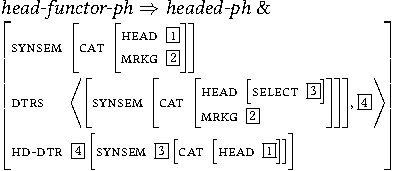
\includegraphics{figures/Ch3132.pdf}
 
\z

\begin{figure}[t]
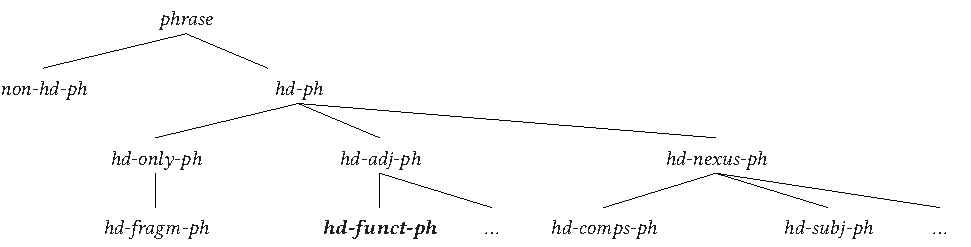
\includegraphics[width=\textwidth]{figures/Ch3Fig7.pdf}  
\caption{Le syntagme tête-foncteur dans une hiérarchie de syntagmes}
\label{ch3:fig7}
\end{figure}




\begin{figure}[t]
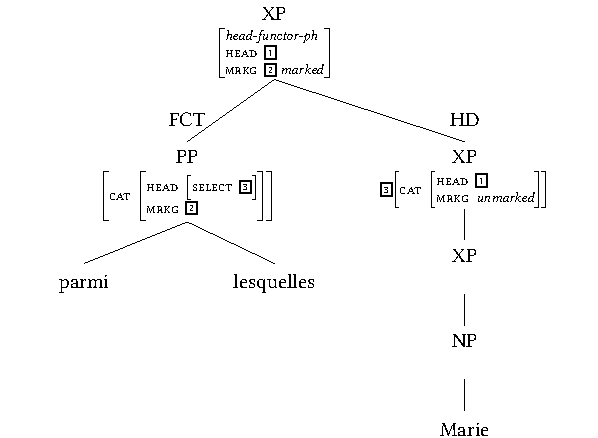
\includegraphics{figures/Ch3Fig8.pdf} % \documentclass[12pt]{article}
\usepackage[latin1]{inputenc}
%\documentclass[twoside,14pt,a4paper]{article}
\usepackage{fullpage}
%\usepackage{times}
\usepackage{latexsym}
\usepackage{ecltree+}
\usepackage{avm}
\usepackage{avm+}
%\usepackage[utf8]{inputenc}
%\usepackage[francais]{babel}

\usepackage{combelow}

\usepackage{xyling}

\begin{document}


\noindent{\textbf{Figure 1 \hspace{1cm} Analyse par reconstruction syntaxique}}
\vspace{1mm}

\Tree[2]{         & \K{\textsc{s}}\B{dl}\B{dr}       & \\
              \K{dont} && \K{\textsc{s}}\B{dl}\B{d}     & \\
               & \K{\textsc{np}}\B{d} & \K{\textsc{vp}}\B{d}\B{dr}\B{drr} & &\\  
       & \K{Marie} & \K{$<$est$>$} & \K{$<$venue$>$} & \K{hier}}


\bigskip



\noindent{\textbf{Figure 2 \hspace{1cm} Analyse en termes de fragment}}
\vspace{1mm}

\Tree[2]{         & \K{\textsc{xp}}\B{dl}\B{dr} &\\  
               \K{dont} && \K{\textsc{xp}}\B{d}\\
       && \K{\textsc{xp}}\B{dl}\B{dr} &\\
      & \K{Marie} && \K{hier}}


\bigskip



\noindent{\textbf{Figure 3 \hspace{1cm} Hi\'erarchie de syntagmes en HPSG, incluant le fragment et le cluster}}
\noindent

\Tree[2] {&& \K[6.2]{\textit{phrase}}\Bkk{6.2,0}{0,0}{dl}\Bkk{6.2,0}{0,0}{drr}		\\
&\K{\textit{non-hd-ph}}\B{dl}\B{dr} &&& \K{\textit{hd-ph}}\B{dl}\B{dr}\B{drrr} \\ 
\K{\textbf{\textit{cluster-ph}}} & &  \K{\textit{coord-ph}} & \K{\textit{hd-only-ph}}\B{d} && \K{\textit{hd-adj-ph}} && \K{\textit{hd-nexus-ph}}\B{dll}\B{dl}\B{d}\B{dr}\\
& & & \K{\textbf{\textit{hd-fragm-ph}}} && \K{\textit{hd-comps}} & \K{\textit{hd-subj}} & \K{\textit{hd-filler}} & \K{\textit{...}}}


%\bigskip
\newpage



\noindent{\textbf{Figure 4 \hspace{1cm} Repr\'esentation simplifi\'ee d'un fragment contenant un cluster de deux constituants}}

\regAvmFonts\avmoptions{center}

\newcommand{\AVMXPone}{\begin{Avm}{XP}
        \[\tp{head-fragment-ph}\\ synsem & \@{2} \[head \@{1}\]\\ mrkg & nil \]
        \end{Avm} }
\newcommand{\AVMXPtwo}{\begin{Avm}{XP}
				\[\tp{cluster-ph} \\ synsem & \@{2} \[head \@{1} & \[cluster & \<\@{3}, \@{4} \> \] \] \] 
				\end{Avm}} 
\newcommand{\AVMNPone}{\begin{Avm}{NP}
    \[synsem & \@{3} \]
\end{Avm}}
\newcommand{\AVMNPtwo}{\begin{Avm}{NP}
    \[synsem & \@{4} \] 
    \end{Avm}}       
    

\smallAvmFonts
\begin{figure}[hbcd]
  \begin{center}
     \begin{bundle}{\AVMXPone}\setlength{\GapDepth}{40pt}
       \chunk[\textsc{hd}]{\setlength{\GapWidth}{45pt}
       		\begin{bundle}{\AVMXPtwo}
               \chunk[\textsc{n-hd}]{\setlength{\GapWidth}{70pt}\setlength{\GapDepth}{20pt}
                  \begin{bundle}{\AVMNPone}
                    \chunk{Marie}
                  \end{bundle}}
               \chunk[\textsc{n-hd}]{\setlength{\GapDepth}{20pt}
                  \begin{bundle}{\AVMNPtwo}
                    \chunk{hier}
                  \end{bundle}}
             \end{bundle}}
             
         \end{bundle}
       	      
    
  \end{center}
\end{figure}
\regAvmFonts


\newpage



\noindent{\textbf{Figure 5 \hspace{1cm} Repr\'esentation simplifi\'ee d'un fragment contenant un cluster unaire}}

\regAvmFonts\avmoptions{center}

\newcommand{\AVMXPthree}{\begin{Avm}{XP}
        \[\tp{head-fragment-ph}\\ synsem & \@{2} \[head \@{1}\]\\ mrkg & nil \]
        \end{Avm} }
\newcommand{\AVMXPfour}{\begin{Avm}{XP}
				\[\tp{cluster-ph} \\ synsem & \@{2} \[head \@{1} & \[cluster & \<\@{3}NP \> \] \] \] 
				\end{Avm}} 
\newcommand{\AVMNPthree}{\begin{Avm}{NP}
    \[synsem & \@{3} \]
\end{Avm}}
          

\smallAvmFonts
\begin{figure}[hbcd]
  \begin{center}
     \begin{bundle}{\AVMXPthree}\setlength{\GapDepth}{40pt}
       \chunk[\textsc{hd}]{\setlength{\GapWidth}{45pt}
       		\begin{bundle}{\AVMXPfour}
               \chunk[\textsc{n-hd}]{\setlength{\GapWidth}{70pt}\setlength{\GapDepth}{20pt}
                  \begin{bundle}{\AVMNPthree}
                    \chunk{Marie}
                  \end{bundle}}
               
             \end{bundle}}
             
         \end{bundle}
       	      
    
  \end{center}
\end{figure}
\regAvmFonts


\bigskip



\noindent{\textbf{Figure 6 \hspace{1cm} Relations fonctionnelles possibles dans la RSV}
\vspace{1mm}

\noindent
\Tree{ &&& \K{\textsc{xp}}\B{dll}_{?}\B{drr}^{HD}  &&&\\
          & \K{\textsc{pp}}\B{dl}\B{dr} & && & \K{\textsc{xp}}\B{d} &\\                         
\K{dintre} && \K{care} &&& \K{\textsc{xp}}\B{dl}\B{dr}\\
&&&&      \K{una} && \K{ieri}}

\paragraph{}

\Tree{&&& \K{\textsc{pp}}\B{dll}_{HD}\B{drr}^{?} &&&\\
          & \K{\textsc{pp}}\B{dl}\B{dr} & && & \K{\textsc{xp}}\B{d} &\\                         
\K{dintre} && \K{care} &&& \K{\textsc{xp}}\B{dl}\B{dr}\\
&&&&      \K{una} && \K{ieri}}

\paragraph{}

\Tree{&&& \K{\textsc{xp}}\B{dll}_{N-HD}\B{drr}^{N-HD} &&&\\
       & \K{\textsc{pp}}\B{dl}\B{dr} & && & \K{\textsc{xp}}\B{d} &\\                         
\K{dintre} && \K{care} &&& \K{\textsc{xp}}\B{dl}\B{dr}\\
&&&&      \K{una} && \K{ieri}}


\bigskip



\noindent{\textbf{Figure 7 \hspace{1cm} Le syntagme de type t\^ete-foncteur dans une hi\'erarchie de syntagmes}

\noindent
\Tree[2]{ & \K[5.2]{\textit{phrase}}\Bkk{5.2,0}{0,0}{dl}\Bkk{5.2,0}{0,0}{dr}		\\
\K{\textit{non-hd-ph}}	&			 & \K[5.2]{\textit{hd-ph}}\Bkk{5.2,0}{0,0}{dl}\Bkk{5.2,0}{0,0}{dr}\Bkk{5.2,0}{0,0}{drrrr}  \\
& \K{\textit{hd-only-ph}}\B{d} & &   \K{\textit{hd-adj-ph}}\B{d}\B{dr} &&& \K{\textit{hd-nexus-ph}}\B{dl}\B{dr}\B{drr}\\
& \K{\textit{hd-fragm-ph}} && \K{\textbf{\textit{hd-funct-ph}}} & \K{\textit{...}} & \K{\textit{hd-comps-ph}} && \K{\textit{hd-subj-ph}} & \K{\textit{...}}}


\bigskip



\noindent{\textbf{Figure 8 \hspace{1cm} Arbre avec un syntagme t\^ete-foncteur}}

\regAvmFonts\avmoptions{center}
\newcommand{\AVMXPfive}{\begin{Avm}{XP}
        \[\tp{head-functor-ph}\\ head & \@{1}\\ mrkg & \@{2} marked\]
      									\end{Avm}}
\newcommand{\AVMPPone}{\begin{Avm}{PP}
        \[cat & \[head & \[select & \@{3}\]\\ mrkg & \@{2}\]\]
      									\end{Avm}}
\newcommand{\AVMXPsix}{\begin{Avm}{XP}
  \@{3}\[cat & \[head & \@{1}\\ mrkg & unmarked\]\]
      									\end{Avm}}
\newcommand{\AVMXPsixbis}{\begin{Avm}{XP} 
        							 \end{Avm}}
\newcommand{\AVMNPfirst}{\begin{Avm}{NP} 
        							 \end{Avm}}


\smallAvmFonts
\begin{figure}[hbcd]
  \begin{center}\setlength{\GapWidth}{60pt}\setlength{\GapDepth}{30pt}
     \begin{bundle}{\AVMXPfive}     	  			
     \chunk[\textsc{fct}]{\setlength{\GapWidth}{60pt}\setlength{\GapDepth}{20pt}
         \begin{bundle}{\AVMPPone}
           \chunk{parmi}
           \chunk{lesquelles}
         \end{bundle}}
     
  		\chunk[\textsc{hd}]{\setlength{\GapWidth}{60pt}\setlength{\GapDepth}{15pt}
         \begin{bundle}{\AVMXPsix}
         	\chunk{\setlength{\GapDepth}{15pt}\begin{bundle}{\AVMXPsixbis}
         	 \chunk{\setlength{\GapDepth}{15pt}\begin{bundle}{\AVMNPfirst}
           \chunk{Marie}
           \end{bundle}}
           \end{bundle}}  
         \end{bundle}}
 
     \end{bundle}
         
  \end{center}
\end{figure}
\regAvmFonts


\newpage



\noindent{\textbf{Figure 9 \hspace{1cm} Syntaxe simplifi\'ee des constructions \`a RSV en fran\c{c}ais}}

\Tree{ &&& \K{\textsc{s}}\B{dll}_{HD}\B{drrr}^{ADJ}  &&\\
& \K{\textsc{s}}\B{dl}_{SUBJ}\B{dr}^{HD} & && && \K{\textsc{xp}}\B{dl}_{FCT}\B{drr}^{HD} &\\ 
\K{\textsc{np}}\TRi && \K{\textsc{v}}\B{d} &&& \K{\textsc{pp}}\B{dl}_{HD}\B{dr}^{COMPS} & && \K{\textsc{xp}}\B{d}^{HD} &\\
\K{plusieurs}\Below{personnes} && \K{chantent} && \K{\textsc{p}rep}\B{d} && \K{\textsc{np}}\TRi && \K{\textsc{xp}}\B{d}^{N-HD}\\
&&&& \K{parmi} && \K{lesquelles} && \K{\textsc{np}}\TRi\\
&&&& && & & \K{Marie}}


\bigskip



\noindent{\textbf{Figure 10 \hspace{1cm} Syntaxe simplifi\'ee des constructions \`a RSV en roumain}}

\Tree{ &&& \K{\textsc{s}}\B{dll}_{HD}\B{drrr}^{ADJ}  &&\\
& \K{\textsc{s}}\B{dl}_{HD}\B{dr}^{SUBJ} & && && \K{\textsc{xp}}\B{dl}_{FCT}\B{drr}^{HD} &\\ 
\K{\textsc{v}}\B{d} && \K{\textsc{np}}\TRi &&& \K{\textsc{pp}}\B{dl}_{HD}\B{dr}^{COMPS} & && \K{\textsc{xp}}\B{d}^{HD} &\\
\K{vin} && \K{mai}\Below{multe}\Below{persoane} && \K{\textsc{p}rep}\B{d} && \K{\textsc{np}}\TRi && \K{\textsc{xp}}\B{d}^{N-HD}\\
&&&& \K{printre} && \K{care} && \K{\textsc{np}}\TRi\\
&&&& && & & \K{\c{s}i Maria}}

  
\newpage



\noindent{\textbf{Figure 11 \hspace{1cm} Relation \`a distance entre l'introducteur et l'\'el\'ement distingu\'e: accessibilit\'e de l'\'el\'ement distingu\'e dans le corps de la RSV}}      									      				

\regAvmFonts\avmoptions{center}
\newcommand{\AVMXPseven}{\begin{Avm}{XP}
        \[\tp{head-functor-ph} \\ ss & \[ head & \@{6} noun \\ mrkg & \@{7} \\ rel & \{\@{4}\} \] \] 
        									\end{Avm}}
        									
\newcommand{\AVMPPtwo}{\begin{Avm}{PP}
        \[\tp{head-comps-ph} \\ ss & \[ head & \[select & \@{1}  \] \\ mrkg & \@{7}\\ rel & \{\@{4}\} \] \] 
        							 \end{Avm}}
        							 
\newcommand{\AVMPrepone}{\begin{Avm}{Prep}
  			\[cat & \[head & \[select & \@{1} \[cont & \[anchors & \<\[ind & \@{3}\]\>\]\]\] \\ mrkg & \@{7}\\ val & \[comps & \<\@{2}\>\] \\ arg-st & \<\@{1}, \@{2}\> \] \\
  			  cont & \[ltop & \@{5} \\ rels & \<\[\tp{sum-subpart-rel} \\ label & \@{5} \\ subpart & \@{3} \\ sum & \@{4} \] \> \] \]
      									\end{Avm}}
      									
\newcommand{\AVMNPfour}{\begin{Avm}{NP}
   \[ss &\@{2}\[cat & \[head & noun\]\\ cont & \[ind & \@{4}\] \\ rel & \{\@{4}\}\] \]
        							 \end{Avm}}

\newcommand{\AVMXPeight}{\begin{Avm}{XP}
   \[\tp{head-fragment-ph} \\ ss &\@{1}\[cat & \[head & \@{6} noun\]\\ cont & \[ind & \@{3}\] \]\] 
        							 \end{Avm}}
        							 
\newcommand{\AVMXPeightbis}{\begin{Avm}{XP} 
        							 \end{Avm}}
\newcommand{\AVMNPsecond}{\begin{Avm}{NP} 
        							 \end{Avm}}        							 

\smallAvmFonts
\begin{figure}[hbcd]
  \begin{center}\setlength{\GapWidth}{100pt}\setlength{\GapDepth}{30pt}
     \begin{bundle}{\AVMXPseven}     	  			
   		\chunk[\textsc{fct}]{\setlength{\GapWidth}{140pt}\setlength{\GapDepth}{20pt}
         \begin{bundle}{\AVMPPtwo}
         	 \chunk[\textsc{hd}]{
         	 	\begin{bundle}{\AVMPrepone}
           		\chunk{parmi}
         		 \end{bundle}}
         	  \chunk[\textsc{comps}]{
         	 	 \begin{bundle}{\AVMNPfour}
           	 	\chunk{lesquelles}
         		 \end{bundle}}
         	\end{bundle}}
       \chunk[\textsc{hd}]{\setlength{\GapDepth}{15pt}
         	 	 \begin{bundle}{\AVMXPeight}
           	 	\chunk{\setlength{\GapDepth}{15pt}\begin{bundle}{\AVMXPeightbis}
         	 \chunk{\setlength{\GapDepth}{15pt}\begin{bundle}{\AVMNPsecond}
           \chunk{Marie}
           \end{bundle}}
           \end{bundle}}
         		 \end{bundle}}
      \end{bundle}
         
  \end{center}
\end{figure}
\regAvmFonts


\newpage



\noindent{\textbf{Figure 12 \hspace{1cm} Relation \`a distance entre la RSV et son ant\'ec\'edent: accessibilit\'e de l'ant\'ec\'edent dans la phrase h\^ote}}

\regAvmFonts\avmoptions{center}
\newcommand{\AVMSone}{\begin{Avm}{S}
        \[\tp{head-functor-ph}\] 
       							 \end{Avm}}
        							 
\newcommand{\AVMStwo}{\begin{Avm}{S}
   \[ss & \@{2}\[cont & \[ind & \@{6} \\ rels & \@{9}\] \] \]
        							 \end{Avm}}
        							 
\newcommand{\AVMNPfive}{\begin{Avm}{NP$_i$}
    	 \[cont & \[ind & \@{4}\] \] 
        							 \end{Avm}}

\newcommand{\AVMVone}{\begin{Avm}{V} 
        							 \end{Avm}}
        							         							 
\newcommand{\AVMXPnine}{\begin{Avm}{XP}
        \[ss & \[cat & \[head & \@{1} \[select & \@{2}\[ cont \[ anchors & \<\[ind & \@{4}\]\>\]\]\] \\
         mrkg & \@{10} \] \\
         cont & \[ind & \@{7}\]\\
         c-cont & \[rels & \<\[\tp{sum-subpart-rel}\\ 
         											subpart & \@{7} event\\
         											sum & \@{6} event\]\>\] \\
											rel & \{\@{4}\}\] \]
        									\end{Avm}}
        									        							 
\newcommand{\AVMPPthree}{\begin{Avm}{PP}
  			 \[ss &\[cat & \[head & \[select & \@{3} \] \\
         mrkg & \@{10} \]\\
			cont & \[ltop & \@{5} \\ rels & \<\[\tp{sum-subpart-rel} \\ label & \@{5} \\ subpart & \@{8} \\ sum & \@{4} \] \> \] \\
			rel & \{\@{4}\}\] \]
      									\end{Avm}}
      									
\newcommand{\AVMXPten}{\begin{Avm}{XP}
   			\[ss &\@{3}\[cat \[head & \@{1}\] \\ 
			cont \[ind  \@{7}\\
   								anchors & \<\[ind & \@{8}\]\>\]\\
   				fragment \[source \[ind & \@{6} \\ rels & \@{9}\]\\
   										abstract-cont \@{B}\]\] \]
        							 \end{Avm}}

\newcommand{\AVMXPtenbis}{\begin{Avm}{XP} 
        							 \end{Avm}}
\newcommand{\AVMNPthird}{\begin{Avm}{NP} 
        							 \end{Avm}}

\smallAvmFonts
\begin{figure}[hbcd]
  \begin{center}\setlength{\GapDepth}{25pt}
     \begin{bundle}{\AVMSone}     	  			
   		\chunk[\textsc{hd}]{
         \begin{bundle}{\AVMStwo}
         	 \chunk[\textsc{subj}]{
         	 	\begin{bundle}{\AVMNPfive}
           		\chunk{plusieurs personnes}
         		 \end{bundle}}
    
         	  \chunk[\textsc{hd}]{
         	 	 \begin{bundle}{\AVMVone}
           	 	\chunk{chantent}
         		 \end{bundle}}
         		 \end{bundle}}
         	
     \chunk[\textsc{fct}]{\setlength{\GapWidth}{110pt}\setlength{\GapDepth}{30pt}
       \begin{bundle}{\AVMXPnine}
         	\chunk[\textsc{fct}]{\setlength{\GapWidth}{30pt}
         	 	\begin{bundle}{\AVMPPthree}
           		\chunk{parmi}
           		\chunk{lesquelles$_i$}
         		 \end{bundle}}
          \chunk[\textsc{hd}]{\setlength{\GapWidth}{20pt}\setlength{\GapDepth}{15pt}
         	 	\begin{bundle}{\AVMXPten}
           	 	\chunk{\setlength{\GapDepth}{15pt}\begin{bundle}{\AVMXPtenbis}
         	 \chunk{\setlength{\GapDepth}{15pt}\begin{bundle}{\AVMNPthird}
           \chunk{Marie}
           \end{bundle}}
           \end{bundle}}
         		 \end{bundle}}	 
         	 \end{bundle}}
         	 	
        \end{bundle}
         
  \end{center}
\end{figure}
\regAvmFonts


\newpage



\noindent{\textbf{Figure 13 \hspace{1cm} Arbre avec le compl\'ementeur \textit{dont} dans les relatives ordinaires}}

\regAvmFonts\avmoptions{center}

\newcommand{\AVMNPsix}{\begin{Avm}{NP}
        \[\tp{head-functor-ph}\]
      \end{Avm}}
\newcommand{\AVMNPseven}{\begin{avm} \@1NP$_i$
      \end{avm}}
\newcommand{\AVMSthree}{\begin{Avm}{S}
    \[head & \[select & \@{1} \] \\ mrkg & dont \\ slash & \{ \} \] 
    \end{Avm}}
\newcommand{\AVMCompr}{\begin{Avm}{Compr}
    \[head & \[vform & \@{2}\]\\ mrkg & dont \\ comps & \<\@{3}\>\\ bind & \{\@{4}\} \\ slash & \{\} \]
		\end{Avm}}
\newcommand{\AVMSfour}{\begin{Avm}{S}
\@{3}\[vform & \@{2} tensed \\ subj & \< \>\\ slash & \{\@{4}PP$_i$[\textit{de}] \}\\ mrkg & unmarked \]
\end{Avm}}
\newcommand{\AVMNPeight}{\begin{Avm}{NP}
    \end{Avm}}
\newcommand{\AVMVtwo}{\begin{Avm}{V}
		\[slash & \{\@{4}\}\]
    \end{Avm}}
    
\smallAvmFonts
\begin{figure}[hbcd]

\begin{center}\setlength{\GapWidth}{40pt}\setlength{\GapDepth}{20pt}
     \begin{bundle}{\AVMNPsix}
     
\chunk[\textsc{hd}]{\setlength{\GapDepth}{30pt}
			\begin{bundle}{\AVMNPseven}
               \chunk{l'histoire}
               \end{bundle}
         }

\chunk[\textsc{fct}]{\setlength{\GapWidth}{80pt}\setlength{\GapDepth}{20pt}
         \begin{bundle}{\AVMSthree}
           \chunk[\textsc{hd}]{
             \begin{bundle}{\AVMCompr}
             		\chunk{dont}
               		\end{bundle}
        			 }
             
               \chunk[\textsc{comps}]{
                  \begin{bundle}{\AVMSfour}
                    \chunk[\textsc{subj}]{
                      \begin{bundle}{\AVMNPeight}
                      \chunk{Marie}
               		\end{bundle}
        			 }
                  
               \chunk[\textsc{hd}]{
                  \begin{bundle}{\AVMVtwo}
                    \chunk{parle}
                  \end{bundle}}
             \end{bundle}
           }
         \end{bundle}
       }
     
     \end{bundle}
  \end{center}
\end{figure}
\regAvmFonts


\newpage



\noindent{\textbf{Figure 14 \hspace{1cm} Arbre avec l'introducteur \textit{dont} dans les RSV}}

\regAvmFonts\avmoptions{center}
\newcommand{\AVMSfive}{\begin{Avm}{S}
        \[\tp{head-functor-ph}\] 
       							 \end{Avm}}
        							 
\newcommand{\AVMSsix}{\begin{Avm}{S}
    \[\tp{head-subject-ph} \\ ss & \@{2}\[cont & \[ind & \@{6}\] \] \]
        							 \end{Avm}}
        							 
\newcommand{\AVMNPnine}{\begin{Avm}{NP}
    	 \[ss & \[cont & \[ind & \@{4}\] \] \] 
        							 \end{Avm}}

\newcommand{\AVMVthree}{\begin{Avm}{V} 
        							 \end{Avm}}
        							         							 
\newcommand{\AVMXPeleven}{\begin{Avm}{XP}
        \[\tp{head-functor-ph} \\ ss & \[cat & \[head \@{1} & \[select & \@{2} \] \\ mrkg & dont \] \] \]
        									\end{Avm}}
        									        							 
\newcommand{\AVMYPone}{\begin{Avm}{?P}
  			\[ss & \[cat & \[head & \[select & \[cat \[head \| select \@{7} \| cont \[anchors & \<\[ind & \@{4}\]\> \] \] \\ cont \[anchors & \<\[ind & \@{3}\]\> \] \] \] \\ mrkg & dont\] \\
  			cont & \[ltop & \@{5} \\ rels & \<\[\tp{sum-subpart-rel} \\ label & \@{5} \\ subpart & \@{3} \\ sum & \@{4} \] \> \] \] \]
      									\end{Avm}}
      									
\newcommand{\AVMXPtwelve}{\begin{Avm}{XP}
   \[\tp{head-fragment-phrase}\\ ss & \@{7}\[cat & \[head & \@{1}\] \\ cont & \[ind & \@{3}\]\] \]
        							 \end{Avm}}

\newcommand{\AVMXPtwelvebis}{\begin{Avm}{XP} 
        							 \end{Avm}}
\newcommand{\AVMNPfourth}{\begin{Avm}{NP} 
        							 \end{Avm}}

\smallAvmFonts
\begin{figure}[hbcd]
  \begin{center}\setlength{\GapWidth}{50pt}\setlength{\GapDepth}{25pt}
     \begin{bundle}{\AVMSfive}     	  			
   		\chunk[\textsc{hd}]{\setlength{\GapWidth}{10pt}
         \begin{bundle}{\AVMSsix}
         	 \chunk[\textsc{subj}]{\setlength{\GapDepth}{15pt}
         	 	\begin{bundle}{\AVMNPnine}
           		\chunk{plusieurs personnes}
         		 \end{bundle}}
    
         	  \chunk[\textsc{hd}]{\setlength{\GapDepth}{19pt}
         	 	 \begin{bundle}{\AVMVthree}
           	 	\chunk{chantent}
         		 \end{bundle}}
         		 \end{bundle}}
         	
     \chunk[\textsc{fct}]{\setlength{\GapWidth}{200pt}\setlength{\GapDepth}{80pt}
       \begin{bundle}{\AVMXPeleven}
         	\chunk[\textsc{fct}]{\setlength{\GapWidth}{100pt}\setlength{\GapDepth}{40pt}
         	 	\begin{bundle}{\AVMYPone}
           		\chunk{dont}
         		 \end{bundle}}
          		\chunk[\textsc{hd}]{\setlength{\GapWidth}{130pt}\setlength{\GapDepth}{15pt}
         	 	\begin{bundle}{\AVMXPtwelve}
           	 	\chunk{\setlength{\GapDepth}{15pt}
           	 	\begin{bundle}{\AVMXPtwelvebis}
         	 \chunk{\setlength{\GapDepth}{15pt}
         	 \begin{bundle}{\AVMNPfourth}
           \chunk{Marie}
           \end{bundle}}
           \end{bundle}}
         		 \end{bundle}}	 
         	 \end{bundle}}
         	 	
        \end{bundle}
         
  \end{center}
\end{figure}
\regAvmFonts


\end{document}
%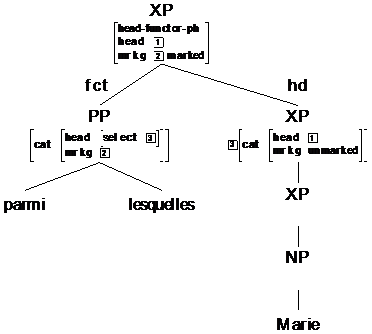
\includegraphics[width=\textwidth]{figures/chap3andconclusion16fevr17-img17.png}
\caption{Arbre avec un syntagme tête-foncteur}
\label{ch3:fig8}
\end{figure}



Les foncteurs ont deux propriétés principales : ils sélectionnent leur tête (cf. le trait SELECT, qui est inclus dans la valeur de HEAD de la branche foncteur) et contribuent au marquage du syntagme (cf. le trait MRKG, qui apparaît dans la valeur du trait CAT). 

Les trois contraintes pesant sur le syntagme tête-foncteur sont :

(i) \is{Principe des traits de tête généralisé}Principe des Traits de Tête : la valeur du trait HEAD d’un syntagme avec tête est identique à la valeur du trait HEAD de la branche tête (on capte ainsi l’intuition générale que la catégorie de la tête donne la catégorie du syntagme). 

(ii) Principe du Sélecteur : on reprend de \citet{VanEynde2003,VanEynde2006,VanEynde2007} le trait SELECT qui capte les contraintes qu’une branche non-tête peut imposer à sa sœur tête. La valeur du trait SELECT de la branche non-tête doit être identique à la valeur SYNSEM de la branche tête. La valeur du trait SELECT est de type \textit{synsem} et non \textit{signe}, ce qui fait que le foncteur peut imposer des contraintes concernant les propriétés syntaxiques et sémantiques de la tête, mais pas concernant les propriétés phonologiques de celle-ci ou encore sa structure interne (ce qui rend possible les différentes constituances au sein du corps de la RSV : un seul constituant ou un \isi{cluster}, par exemple). La raison pour laquelle le trait SELECT est introduit dans la valeur du trait HEAD du foncteur est le fait que les propriétés de sélection d’un foncteur syntagmatique sont identiques à celles de sa branche tête.

(iii) Principe du Marquage Généralisé : l’information qui figure dans la valeur du trait MARKING est partagée entre la mère et sa branche non-tête (la valeur MARKING de la mère dans un syntagme de type \textit{hd-funct-ph} est identique à celle de sa branche non-tête).  

Le syntagme tête-foncteur présente ainsi deux branches : une branche tête (dont l’indice est \fbox{3} en \REF{ch3:ex132} et \figref{ch3:fig8}) qui donne le trait HEAD de la construction, et une branche foncteur qui sélectionne sa tête et contribue au marquage de la construction. Par conséquent, la tête d’une RSV est le fragment tel qu’il a été défini dans les sections~\ref{ch3:sect3.5.1} et~\ref{ch3:sect3.5.2}.

\largerpage 
Après avoir défini les relations syntaxiques qui s’établissent (i) à l’intérieur du corps d’une RSV, (ii) entre le corps de la RSV et l’introducteur, et (iii) entre la RSV dans son ensemble et la phrase hôte, on peut donner une représentation simplifiée de ces relations en \figref{ch3:fig9} pour le français et en \figref{ch3:fig10} pour le roumain. L’arbre donné en \figref{ch3:fig10} est une illustration de l’exemple roumain \REF{ch3:ex133}. 

\begin{figure}
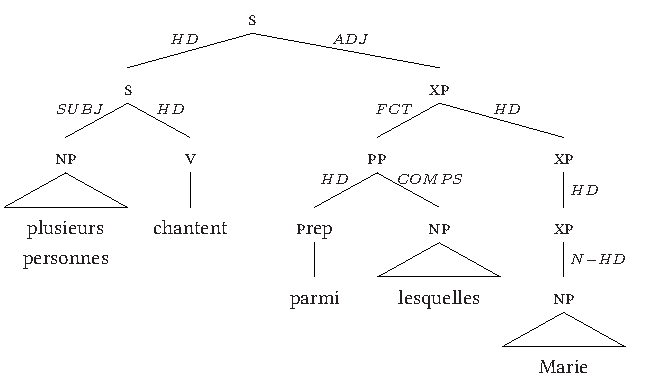
\includegraphics{figures/Ch3Fig9.pdf} % \documentclass[12pt]{article}
\usepackage[latin1]{inputenc}
%\documentclass[twoside,14pt,a4paper]{article}
\usepackage{fullpage}
%\usepackage{times}
\usepackage{latexsym}
\usepackage{ecltree+}
\usepackage{avm}
\usepackage{avm+}
%\usepackage[utf8]{inputenc}
%\usepackage[francais]{babel}

\usepackage{combelow}

\usepackage{xyling}

\begin{document}


\noindent{\textbf{Figure 1 \hspace{1cm} Analyse par reconstruction syntaxique}}
\vspace{1mm}

\Tree[2]{         & \K{\textsc{s}}\B{dl}\B{dr}       & \\
              \K{dont} && \K{\textsc{s}}\B{dl}\B{d}     & \\
               & \K{\textsc{np}}\B{d} & \K{\textsc{vp}}\B{d}\B{dr}\B{drr} & &\\  
       & \K{Marie} & \K{$<$est$>$} & \K{$<$venue$>$} & \K{hier}}


\bigskip



\noindent{\textbf{Figure 2 \hspace{1cm} Analyse en termes de fragment}}
\vspace{1mm}

\Tree[2]{         & \K{\textsc{xp}}\B{dl}\B{dr} &\\  
               \K{dont} && \K{\textsc{xp}}\B{d}\\
       && \K{\textsc{xp}}\B{dl}\B{dr} &\\
      & \K{Marie} && \K{hier}}


\bigskip



\noindent{\textbf{Figure 3 \hspace{1cm} Hi\'erarchie de syntagmes en HPSG, incluant le fragment et le cluster}}
\noindent

\Tree[2] {&& \K[6.2]{\textit{phrase}}\Bkk{6.2,0}{0,0}{dl}\Bkk{6.2,0}{0,0}{drr}		\\
&\K{\textit{non-hd-ph}}\B{dl}\B{dr} &&& \K{\textit{hd-ph}}\B{dl}\B{dr}\B{drrr} \\ 
\K{\textbf{\textit{cluster-ph}}} & &  \K{\textit{coord-ph}} & \K{\textit{hd-only-ph}}\B{d} && \K{\textit{hd-adj-ph}} && \K{\textit{hd-nexus-ph}}\B{dll}\B{dl}\B{d}\B{dr}\\
& & & \K{\textbf{\textit{hd-fragm-ph}}} && \K{\textit{hd-comps}} & \K{\textit{hd-subj}} & \K{\textit{hd-filler}} & \K{\textit{...}}}


%\bigskip
\newpage



\noindent{\textbf{Figure 4 \hspace{1cm} Repr\'esentation simplifi\'ee d'un fragment contenant un cluster de deux constituants}}

\regAvmFonts\avmoptions{center}

\newcommand{\AVMXPone}{\begin{Avm}{XP}
        \[\tp{head-fragment-ph}\\ synsem & \@{2} \[head \@{1}\]\\ mrkg & nil \]
        \end{Avm} }
\newcommand{\AVMXPtwo}{\begin{Avm}{XP}
				\[\tp{cluster-ph} \\ synsem & \@{2} \[head \@{1} & \[cluster & \<\@{3}, \@{4} \> \] \] \] 
				\end{Avm}} 
\newcommand{\AVMNPone}{\begin{Avm}{NP}
    \[synsem & \@{3} \]
\end{Avm}}
\newcommand{\AVMNPtwo}{\begin{Avm}{NP}
    \[synsem & \@{4} \] 
    \end{Avm}}       
    

\smallAvmFonts
\begin{figure}[hbcd]
  \begin{center}
     \begin{bundle}{\AVMXPone}\setlength{\GapDepth}{40pt}
       \chunk[\textsc{hd}]{\setlength{\GapWidth}{45pt}
       		\begin{bundle}{\AVMXPtwo}
               \chunk[\textsc{n-hd}]{\setlength{\GapWidth}{70pt}\setlength{\GapDepth}{20pt}
                  \begin{bundle}{\AVMNPone}
                    \chunk{Marie}
                  \end{bundle}}
               \chunk[\textsc{n-hd}]{\setlength{\GapDepth}{20pt}
                  \begin{bundle}{\AVMNPtwo}
                    \chunk{hier}
                  \end{bundle}}
             \end{bundle}}
             
         \end{bundle}
       	      
    
  \end{center}
\end{figure}
\regAvmFonts


\newpage



\noindent{\textbf{Figure 5 \hspace{1cm} Repr\'esentation simplifi\'ee d'un fragment contenant un cluster unaire}}

\regAvmFonts\avmoptions{center}

\newcommand{\AVMXPthree}{\begin{Avm}{XP}
        \[\tp{head-fragment-ph}\\ synsem & \@{2} \[head \@{1}\]\\ mrkg & nil \]
        \end{Avm} }
\newcommand{\AVMXPfour}{\begin{Avm}{XP}
				\[\tp{cluster-ph} \\ synsem & \@{2} \[head \@{1} & \[cluster & \<\@{3}NP \> \] \] \] 
				\end{Avm}} 
\newcommand{\AVMNPthree}{\begin{Avm}{NP}
    \[synsem & \@{3} \]
\end{Avm}}
          

\smallAvmFonts
\begin{figure}[hbcd]
  \begin{center}
     \begin{bundle}{\AVMXPthree}\setlength{\GapDepth}{40pt}
       \chunk[\textsc{hd}]{\setlength{\GapWidth}{45pt}
       		\begin{bundle}{\AVMXPfour}
               \chunk[\textsc{n-hd}]{\setlength{\GapWidth}{70pt}\setlength{\GapDepth}{20pt}
                  \begin{bundle}{\AVMNPthree}
                    \chunk{Marie}
                  \end{bundle}}
               
             \end{bundle}}
             
         \end{bundle}
       	      
    
  \end{center}
\end{figure}
\regAvmFonts


\bigskip



\noindent{\textbf{Figure 6 \hspace{1cm} Relations fonctionnelles possibles dans la RSV}
\vspace{1mm}

\noindent
\Tree{ &&& \K{\textsc{xp}}\B{dll}_{?}\B{drr}^{HD}  &&&\\
          & \K{\textsc{pp}}\B{dl}\B{dr} & && & \K{\textsc{xp}}\B{d} &\\                         
\K{dintre} && \K{care} &&& \K{\textsc{xp}}\B{dl}\B{dr}\\
&&&&      \K{una} && \K{ieri}}

\paragraph{}

\Tree{&&& \K{\textsc{pp}}\B{dll}_{HD}\B{drr}^{?} &&&\\
          & \K{\textsc{pp}}\B{dl}\B{dr} & && & \K{\textsc{xp}}\B{d} &\\                         
\K{dintre} && \K{care} &&& \K{\textsc{xp}}\B{dl}\B{dr}\\
&&&&      \K{una} && \K{ieri}}

\paragraph{}

\Tree{&&& \K{\textsc{xp}}\B{dll}_{N-HD}\B{drr}^{N-HD} &&&\\
       & \K{\textsc{pp}}\B{dl}\B{dr} & && & \K{\textsc{xp}}\B{d} &\\                         
\K{dintre} && \K{care} &&& \K{\textsc{xp}}\B{dl}\B{dr}\\
&&&&      \K{una} && \K{ieri}}


\bigskip



\noindent{\textbf{Figure 7 \hspace{1cm} Le syntagme de type t\^ete-foncteur dans une hi\'erarchie de syntagmes}

\noindent
\Tree[2]{ & \K[5.2]{\textit{phrase}}\Bkk{5.2,0}{0,0}{dl}\Bkk{5.2,0}{0,0}{dr}		\\
\K{\textit{non-hd-ph}}	&			 & \K[5.2]{\textit{hd-ph}}\Bkk{5.2,0}{0,0}{dl}\Bkk{5.2,0}{0,0}{dr}\Bkk{5.2,0}{0,0}{drrrr}  \\
& \K{\textit{hd-only-ph}}\B{d} & &   \K{\textit{hd-adj-ph}}\B{d}\B{dr} &&& \K{\textit{hd-nexus-ph}}\B{dl}\B{dr}\B{drr}\\
& \K{\textit{hd-fragm-ph}} && \K{\textbf{\textit{hd-funct-ph}}} & \K{\textit{...}} & \K{\textit{hd-comps-ph}} && \K{\textit{hd-subj-ph}} & \K{\textit{...}}}


\bigskip



\noindent{\textbf{Figure 8 \hspace{1cm} Arbre avec un syntagme t\^ete-foncteur}}

\regAvmFonts\avmoptions{center}
\newcommand{\AVMXPfive}{\begin{Avm}{XP}
        \[\tp{head-functor-ph}\\ head & \@{1}\\ mrkg & \@{2} marked\]
      									\end{Avm}}
\newcommand{\AVMPPone}{\begin{Avm}{PP}
        \[cat & \[head & \[select & \@{3}\]\\ mrkg & \@{2}\]\]
      									\end{Avm}}
\newcommand{\AVMXPsix}{\begin{Avm}{XP}
  \@{3}\[cat & \[head & \@{1}\\ mrkg & unmarked\]\]
      									\end{Avm}}
\newcommand{\AVMXPsixbis}{\begin{Avm}{XP} 
        							 \end{Avm}}
\newcommand{\AVMNPfirst}{\begin{Avm}{NP} 
        							 \end{Avm}}


\smallAvmFonts
\begin{figure}[hbcd]
  \begin{center}\setlength{\GapWidth}{60pt}\setlength{\GapDepth}{30pt}
     \begin{bundle}{\AVMXPfive}     	  			
     \chunk[\textsc{fct}]{\setlength{\GapWidth}{60pt}\setlength{\GapDepth}{20pt}
         \begin{bundle}{\AVMPPone}
           \chunk{parmi}
           \chunk{lesquelles}
         \end{bundle}}
     
  		\chunk[\textsc{hd}]{\setlength{\GapWidth}{60pt}\setlength{\GapDepth}{15pt}
         \begin{bundle}{\AVMXPsix}
         	\chunk{\setlength{\GapDepth}{15pt}\begin{bundle}{\AVMXPsixbis}
         	 \chunk{\setlength{\GapDepth}{15pt}\begin{bundle}{\AVMNPfirst}
           \chunk{Marie}
           \end{bundle}}
           \end{bundle}}  
         \end{bundle}}
 
     \end{bundle}
         
  \end{center}
\end{figure}
\regAvmFonts


\newpage



\noindent{\textbf{Figure 9 \hspace{1cm} Syntaxe simplifi\'ee des constructions \`a RSV en fran\c{c}ais}}

\Tree{ &&& \K{\textsc{s}}\B{dll}_{HD}\B{drrr}^{ADJ}  &&\\
& \K{\textsc{s}}\B{dl}_{SUBJ}\B{dr}^{HD} & && && \K{\textsc{xp}}\B{dl}_{FCT}\B{drr}^{HD} &\\ 
\K{\textsc{np}}\TRi && \K{\textsc{v}}\B{d} &&& \K{\textsc{pp}}\B{dl}_{HD}\B{dr}^{COMPS} & && \K{\textsc{xp}}\B{d}^{HD} &\\
\K{plusieurs}\Below{personnes} && \K{chantent} && \K{\textsc{p}rep}\B{d} && \K{\textsc{np}}\TRi && \K{\textsc{xp}}\B{d}^{N-HD}\\
&&&& \K{parmi} && \K{lesquelles} && \K{\textsc{np}}\TRi\\
&&&& && & & \K{Marie}}


\bigskip



\noindent{\textbf{Figure 10 \hspace{1cm} Syntaxe simplifi\'ee des constructions \`a RSV en roumain}}

\Tree{ &&& \K{\textsc{s}}\B{dll}_{HD}\B{drrr}^{ADJ}  &&\\
& \K{\textsc{s}}\B{dl}_{HD}\B{dr}^{SUBJ} & && && \K{\textsc{xp}}\B{dl}_{FCT}\B{drr}^{HD} &\\ 
\K{\textsc{v}}\B{d} && \K{\textsc{np}}\TRi &&& \K{\textsc{pp}}\B{dl}_{HD}\B{dr}^{COMPS} & && \K{\textsc{xp}}\B{d}^{HD} &\\
\K{vin} && \K{mai}\Below{multe}\Below{persoane} && \K{\textsc{p}rep}\B{d} && \K{\textsc{np}}\TRi && \K{\textsc{xp}}\B{d}^{N-HD}\\
&&&& \K{printre} && \K{care} && \K{\textsc{np}}\TRi\\
&&&& && & & \K{\c{s}i Maria}}

  
\newpage



\noindent{\textbf{Figure 11 \hspace{1cm} Relation \`a distance entre l'introducteur et l'\'el\'ement distingu\'e: accessibilit\'e de l'\'el\'ement distingu\'e dans le corps de la RSV}}      									      				

\regAvmFonts\avmoptions{center}
\newcommand{\AVMXPseven}{\begin{Avm}{XP}
        \[\tp{head-functor-ph} \\ ss & \[ head & \@{6} noun \\ mrkg & \@{7} \\ rel & \{\@{4}\} \] \] 
        									\end{Avm}}
        									
\newcommand{\AVMPPtwo}{\begin{Avm}{PP}
        \[\tp{head-comps-ph} \\ ss & \[ head & \[select & \@{1}  \] \\ mrkg & \@{7}\\ rel & \{\@{4}\} \] \] 
        							 \end{Avm}}
        							 
\newcommand{\AVMPrepone}{\begin{Avm}{Prep}
  			\[cat & \[head & \[select & \@{1} \[cont & \[anchors & \<\[ind & \@{3}\]\>\]\]\] \\ mrkg & \@{7}\\ val & \[comps & \<\@{2}\>\] \\ arg-st & \<\@{1}, \@{2}\> \] \\
  			  cont & \[ltop & \@{5} \\ rels & \<\[\tp{sum-subpart-rel} \\ label & \@{5} \\ subpart & \@{3} \\ sum & \@{4} \] \> \] \]
      									\end{Avm}}
      									
\newcommand{\AVMNPfour}{\begin{Avm}{NP}
   \[ss &\@{2}\[cat & \[head & noun\]\\ cont & \[ind & \@{4}\] \\ rel & \{\@{4}\}\] \]
        							 \end{Avm}}

\newcommand{\AVMXPeight}{\begin{Avm}{XP}
   \[\tp{head-fragment-ph} \\ ss &\@{1}\[cat & \[head & \@{6} noun\]\\ cont & \[ind & \@{3}\] \]\] 
        							 \end{Avm}}
        							 
\newcommand{\AVMXPeightbis}{\begin{Avm}{XP} 
        							 \end{Avm}}
\newcommand{\AVMNPsecond}{\begin{Avm}{NP} 
        							 \end{Avm}}        							 

\smallAvmFonts
\begin{figure}[hbcd]
  \begin{center}\setlength{\GapWidth}{100pt}\setlength{\GapDepth}{30pt}
     \begin{bundle}{\AVMXPseven}     	  			
   		\chunk[\textsc{fct}]{\setlength{\GapWidth}{140pt}\setlength{\GapDepth}{20pt}
         \begin{bundle}{\AVMPPtwo}
         	 \chunk[\textsc{hd}]{
         	 	\begin{bundle}{\AVMPrepone}
           		\chunk{parmi}
         		 \end{bundle}}
         	  \chunk[\textsc{comps}]{
         	 	 \begin{bundle}{\AVMNPfour}
           	 	\chunk{lesquelles}
         		 \end{bundle}}
         	\end{bundle}}
       \chunk[\textsc{hd}]{\setlength{\GapDepth}{15pt}
         	 	 \begin{bundle}{\AVMXPeight}
           	 	\chunk{\setlength{\GapDepth}{15pt}\begin{bundle}{\AVMXPeightbis}
         	 \chunk{\setlength{\GapDepth}{15pt}\begin{bundle}{\AVMNPsecond}
           \chunk{Marie}
           \end{bundle}}
           \end{bundle}}
         		 \end{bundle}}
      \end{bundle}
         
  \end{center}
\end{figure}
\regAvmFonts


\newpage



\noindent{\textbf{Figure 12 \hspace{1cm} Relation \`a distance entre la RSV et son ant\'ec\'edent: accessibilit\'e de l'ant\'ec\'edent dans la phrase h\^ote}}

\regAvmFonts\avmoptions{center}
\newcommand{\AVMSone}{\begin{Avm}{S}
        \[\tp{head-functor-ph}\] 
       							 \end{Avm}}
        							 
\newcommand{\AVMStwo}{\begin{Avm}{S}
   \[ss & \@{2}\[cont & \[ind & \@{6} \\ rels & \@{9}\] \] \]
        							 \end{Avm}}
        							 
\newcommand{\AVMNPfive}{\begin{Avm}{NP$_i$}
    	 \[cont & \[ind & \@{4}\] \] 
        							 \end{Avm}}

\newcommand{\AVMVone}{\begin{Avm}{V} 
        							 \end{Avm}}
        							         							 
\newcommand{\AVMXPnine}{\begin{Avm}{XP}
        \[ss & \[cat & \[head & \@{1} \[select & \@{2}\[ cont \[ anchors & \<\[ind & \@{4}\]\>\]\]\] \\
         mrkg & \@{10} \] \\
         cont & \[ind & \@{7}\]\\
         c-cont & \[rels & \<\[\tp{sum-subpart-rel}\\ 
         											subpart & \@{7} event\\
         											sum & \@{6} event\]\>\] \\
											rel & \{\@{4}\}\] \]
        									\end{Avm}}
        									        							 
\newcommand{\AVMPPthree}{\begin{Avm}{PP}
  			 \[ss &\[cat & \[head & \[select & \@{3} \] \\
         mrkg & \@{10} \]\\
			cont & \[ltop & \@{5} \\ rels & \<\[\tp{sum-subpart-rel} \\ label & \@{5} \\ subpart & \@{8} \\ sum & \@{4} \] \> \] \\
			rel & \{\@{4}\}\] \]
      									\end{Avm}}
      									
\newcommand{\AVMXPten}{\begin{Avm}{XP}
   			\[ss &\@{3}\[cat \[head & \@{1}\] \\ 
			cont \[ind  \@{7}\\
   								anchors & \<\[ind & \@{8}\]\>\]\\
   				fragment \[source \[ind & \@{6} \\ rels & \@{9}\]\\
   										abstract-cont \@{B}\]\] \]
        							 \end{Avm}}

\newcommand{\AVMXPtenbis}{\begin{Avm}{XP} 
        							 \end{Avm}}
\newcommand{\AVMNPthird}{\begin{Avm}{NP} 
        							 \end{Avm}}

\smallAvmFonts
\begin{figure}[hbcd]
  \begin{center}\setlength{\GapDepth}{25pt}
     \begin{bundle}{\AVMSone}     	  			
   		\chunk[\textsc{hd}]{
         \begin{bundle}{\AVMStwo}
         	 \chunk[\textsc{subj}]{
         	 	\begin{bundle}{\AVMNPfive}
           		\chunk{plusieurs personnes}
         		 \end{bundle}}
    
         	  \chunk[\textsc{hd}]{
         	 	 \begin{bundle}{\AVMVone}
           	 	\chunk{chantent}
         		 \end{bundle}}
         		 \end{bundle}}
         	
     \chunk[\textsc{fct}]{\setlength{\GapWidth}{110pt}\setlength{\GapDepth}{30pt}
       \begin{bundle}{\AVMXPnine}
         	\chunk[\textsc{fct}]{\setlength{\GapWidth}{30pt}
         	 	\begin{bundle}{\AVMPPthree}
           		\chunk{parmi}
           		\chunk{lesquelles$_i$}
         		 \end{bundle}}
          \chunk[\textsc{hd}]{\setlength{\GapWidth}{20pt}\setlength{\GapDepth}{15pt}
         	 	\begin{bundle}{\AVMXPten}
           	 	\chunk{\setlength{\GapDepth}{15pt}\begin{bundle}{\AVMXPtenbis}
         	 \chunk{\setlength{\GapDepth}{15pt}\begin{bundle}{\AVMNPthird}
           \chunk{Marie}
           \end{bundle}}
           \end{bundle}}
         		 \end{bundle}}	 
         	 \end{bundle}}
         	 	
        \end{bundle}
         
  \end{center}
\end{figure}
\regAvmFonts


\newpage



\noindent{\textbf{Figure 13 \hspace{1cm} Arbre avec le compl\'ementeur \textit{dont} dans les relatives ordinaires}}

\regAvmFonts\avmoptions{center}

\newcommand{\AVMNPsix}{\begin{Avm}{NP}
        \[\tp{head-functor-ph}\]
      \end{Avm}}
\newcommand{\AVMNPseven}{\begin{avm} \@1NP$_i$
      \end{avm}}
\newcommand{\AVMSthree}{\begin{Avm}{S}
    \[head & \[select & \@{1} \] \\ mrkg & dont \\ slash & \{ \} \] 
    \end{Avm}}
\newcommand{\AVMCompr}{\begin{Avm}{Compr}
    \[head & \[vform & \@{2}\]\\ mrkg & dont \\ comps & \<\@{3}\>\\ bind & \{\@{4}\} \\ slash & \{\} \]
		\end{Avm}}
\newcommand{\AVMSfour}{\begin{Avm}{S}
\@{3}\[vform & \@{2} tensed \\ subj & \< \>\\ slash & \{\@{4}PP$_i$[\textit{de}] \}\\ mrkg & unmarked \]
\end{Avm}}
\newcommand{\AVMNPeight}{\begin{Avm}{NP}
    \end{Avm}}
\newcommand{\AVMVtwo}{\begin{Avm}{V}
		\[slash & \{\@{4}\}\]
    \end{Avm}}
    
\smallAvmFonts
\begin{figure}[hbcd]

\begin{center}\setlength{\GapWidth}{40pt}\setlength{\GapDepth}{20pt}
     \begin{bundle}{\AVMNPsix}
     
\chunk[\textsc{hd}]{\setlength{\GapDepth}{30pt}
			\begin{bundle}{\AVMNPseven}
               \chunk{l'histoire}
               \end{bundle}
         }

\chunk[\textsc{fct}]{\setlength{\GapWidth}{80pt}\setlength{\GapDepth}{20pt}
         \begin{bundle}{\AVMSthree}
           \chunk[\textsc{hd}]{
             \begin{bundle}{\AVMCompr}
             		\chunk{dont}
               		\end{bundle}
        			 }
             
               \chunk[\textsc{comps}]{
                  \begin{bundle}{\AVMSfour}
                    \chunk[\textsc{subj}]{
                      \begin{bundle}{\AVMNPeight}
                      \chunk{Marie}
               		\end{bundle}
        			 }
                  
               \chunk[\textsc{hd}]{
                  \begin{bundle}{\AVMVtwo}
                    \chunk{parle}
                  \end{bundle}}
             \end{bundle}
           }
         \end{bundle}
       }
     
     \end{bundle}
  \end{center}
\end{figure}
\regAvmFonts


\newpage



\noindent{\textbf{Figure 14 \hspace{1cm} Arbre avec l'introducteur \textit{dont} dans les RSV}}

\regAvmFonts\avmoptions{center}
\newcommand{\AVMSfive}{\begin{Avm}{S}
        \[\tp{head-functor-ph}\] 
       							 \end{Avm}}
        							 
\newcommand{\AVMSsix}{\begin{Avm}{S}
    \[\tp{head-subject-ph} \\ ss & \@{2}\[cont & \[ind & \@{6}\] \] \]
        							 \end{Avm}}
        							 
\newcommand{\AVMNPnine}{\begin{Avm}{NP}
    	 \[ss & \[cont & \[ind & \@{4}\] \] \] 
        							 \end{Avm}}

\newcommand{\AVMVthree}{\begin{Avm}{V} 
        							 \end{Avm}}
        							         							 
\newcommand{\AVMXPeleven}{\begin{Avm}{XP}
        \[\tp{head-functor-ph} \\ ss & \[cat & \[head \@{1} & \[select & \@{2} \] \\ mrkg & dont \] \] \]
        									\end{Avm}}
        									        							 
\newcommand{\AVMYPone}{\begin{Avm}{?P}
  			\[ss & \[cat & \[head & \[select & \[cat \[head \| select \@{7} \| cont \[anchors & \<\[ind & \@{4}\]\> \] \] \\ cont \[anchors & \<\[ind & \@{3}\]\> \] \] \] \\ mrkg & dont\] \\
  			cont & \[ltop & \@{5} \\ rels & \<\[\tp{sum-subpart-rel} \\ label & \@{5} \\ subpart & \@{3} \\ sum & \@{4} \] \> \] \] \]
      									\end{Avm}}
      									
\newcommand{\AVMXPtwelve}{\begin{Avm}{XP}
   \[\tp{head-fragment-phrase}\\ ss & \@{7}\[cat & \[head & \@{1}\] \\ cont & \[ind & \@{3}\]\] \]
        							 \end{Avm}}

\newcommand{\AVMXPtwelvebis}{\begin{Avm}{XP} 
        							 \end{Avm}}
\newcommand{\AVMNPfourth}{\begin{Avm}{NP} 
        							 \end{Avm}}

\smallAvmFonts
\begin{figure}[hbcd]
  \begin{center}\setlength{\GapWidth}{50pt}\setlength{\GapDepth}{25pt}
     \begin{bundle}{\AVMSfive}     	  			
   		\chunk[\textsc{hd}]{\setlength{\GapWidth}{10pt}
         \begin{bundle}{\AVMSsix}
         	 \chunk[\textsc{subj}]{\setlength{\GapDepth}{15pt}
         	 	\begin{bundle}{\AVMNPnine}
           		\chunk{plusieurs personnes}
         		 \end{bundle}}
    
         	  \chunk[\textsc{hd}]{\setlength{\GapDepth}{19pt}
         	 	 \begin{bundle}{\AVMVthree}
           	 	\chunk{chantent}
         		 \end{bundle}}
         		 \end{bundle}}
         	
     \chunk[\textsc{fct}]{\setlength{\GapWidth}{200pt}\setlength{\GapDepth}{80pt}
       \begin{bundle}{\AVMXPeleven}
         	\chunk[\textsc{fct}]{\setlength{\GapWidth}{100pt}\setlength{\GapDepth}{40pt}
         	 	\begin{bundle}{\AVMYPone}
           		\chunk{dont}
         		 \end{bundle}}
          		\chunk[\textsc{hd}]{\setlength{\GapWidth}{130pt}\setlength{\GapDepth}{15pt}
         	 	\begin{bundle}{\AVMXPtwelve}
           	 	\chunk{\setlength{\GapDepth}{15pt}
           	 	\begin{bundle}{\AVMXPtwelvebis}
         	 \chunk{\setlength{\GapDepth}{15pt}
         	 \begin{bundle}{\AVMNPfourth}
           \chunk{Marie}
           \end{bundle}}
           \end{bundle}}
         		 \end{bundle}}	 
         	 \end{bundle}}
         	 	
        \end{bundle}
         
  \end{center}
\end{figure}
\regAvmFonts


\end{document}
%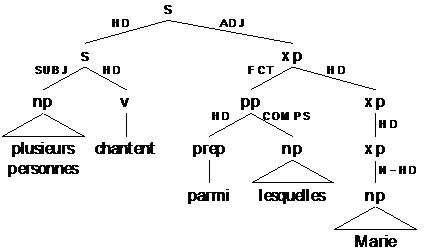
\includegraphics[width=\textwidth]{figures/chap3andconclusion16fevr17-img18.png}
\caption{Syntaxe simplifiée des constructions avec RSV en français}
\label{ch3:fig9}
\end{figure}

\begin{figure}
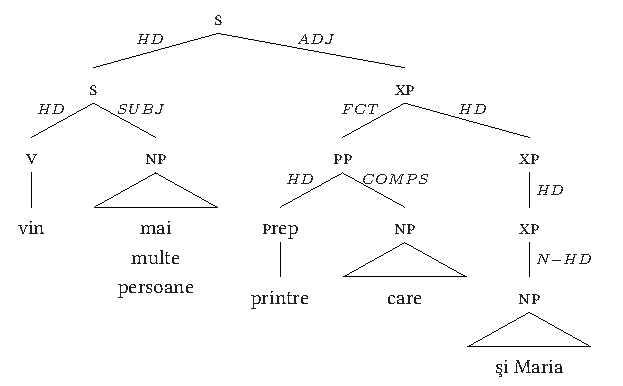
\includegraphics{figures/Ch3Fig10.pdf} % \documentclass[12pt]{article}
\usepackage[latin1]{inputenc}
%\documentclass[twoside,14pt,a4paper]{article}
\usepackage{fullpage}
%\usepackage{times}
\usepackage{latexsym}
\usepackage{ecltree+}
\usepackage{avm}
\usepackage{avm+}
%\usepackage[utf8]{inputenc}
%\usepackage[francais]{babel}

\usepackage{combelow}

\usepackage{xyling}

\begin{document}


\noindent{\textbf{Figure 1 \hspace{1cm} Analyse par reconstruction syntaxique}}
\vspace{1mm}

\Tree[2]{         & \K{\textsc{s}}\B{dl}\B{dr}       & \\
              \K{dont} && \K{\textsc{s}}\B{dl}\B{d}     & \\
               & \K{\textsc{np}}\B{d} & \K{\textsc{vp}}\B{d}\B{dr}\B{drr} & &\\  
       & \K{Marie} & \K{$<$est$>$} & \K{$<$venue$>$} & \K{hier}}


\bigskip



\noindent{\textbf{Figure 2 \hspace{1cm} Analyse en termes de fragment}}
\vspace{1mm}

\Tree[2]{         & \K{\textsc{xp}}\B{dl}\B{dr} &\\  
               \K{dont} && \K{\textsc{xp}}\B{d}\\
       && \K{\textsc{xp}}\B{dl}\B{dr} &\\
      & \K{Marie} && \K{hier}}


\bigskip



\noindent{\textbf{Figure 3 \hspace{1cm} Hi\'erarchie de syntagmes en HPSG, incluant le fragment et le cluster}}
\noindent

\Tree[2] {&& \K[6.2]{\textit{phrase}}\Bkk{6.2,0}{0,0}{dl}\Bkk{6.2,0}{0,0}{drr}		\\
&\K{\textit{non-hd-ph}}\B{dl}\B{dr} &&& \K{\textit{hd-ph}}\B{dl}\B{dr}\B{drrr} \\ 
\K{\textbf{\textit{cluster-ph}}} & &  \K{\textit{coord-ph}} & \K{\textit{hd-only-ph}}\B{d} && \K{\textit{hd-adj-ph}} && \K{\textit{hd-nexus-ph}}\B{dll}\B{dl}\B{d}\B{dr}\\
& & & \K{\textbf{\textit{hd-fragm-ph}}} && \K{\textit{hd-comps}} & \K{\textit{hd-subj}} & \K{\textit{hd-filler}} & \K{\textit{...}}}


%\bigskip
\newpage



\noindent{\textbf{Figure 4 \hspace{1cm} Repr\'esentation simplifi\'ee d'un fragment contenant un cluster de deux constituants}}

\regAvmFonts\avmoptions{center}

\newcommand{\AVMXPone}{\begin{Avm}{XP}
        \[\tp{head-fragment-ph}\\ synsem & \@{2} \[head \@{1}\]\\ mrkg & nil \]
        \end{Avm} }
\newcommand{\AVMXPtwo}{\begin{Avm}{XP}
				\[\tp{cluster-ph} \\ synsem & \@{2} \[head \@{1} & \[cluster & \<\@{3}, \@{4} \> \] \] \] 
				\end{Avm}} 
\newcommand{\AVMNPone}{\begin{Avm}{NP}
    \[synsem & \@{3} \]
\end{Avm}}
\newcommand{\AVMNPtwo}{\begin{Avm}{NP}
    \[synsem & \@{4} \] 
    \end{Avm}}       
    

\smallAvmFonts
\begin{figure}[hbcd]
  \begin{center}
     \begin{bundle}{\AVMXPone}\setlength{\GapDepth}{40pt}
       \chunk[\textsc{hd}]{\setlength{\GapWidth}{45pt}
       		\begin{bundle}{\AVMXPtwo}
               \chunk[\textsc{n-hd}]{\setlength{\GapWidth}{70pt}\setlength{\GapDepth}{20pt}
                  \begin{bundle}{\AVMNPone}
                    \chunk{Marie}
                  \end{bundle}}
               \chunk[\textsc{n-hd}]{\setlength{\GapDepth}{20pt}
                  \begin{bundle}{\AVMNPtwo}
                    \chunk{hier}
                  \end{bundle}}
             \end{bundle}}
             
         \end{bundle}
       	      
    
  \end{center}
\end{figure}
\regAvmFonts


\newpage



\noindent{\textbf{Figure 5 \hspace{1cm} Repr\'esentation simplifi\'ee d'un fragment contenant un cluster unaire}}

\regAvmFonts\avmoptions{center}

\newcommand{\AVMXPthree}{\begin{Avm}{XP}
        \[\tp{head-fragment-ph}\\ synsem & \@{2} \[head \@{1}\]\\ mrkg & nil \]
        \end{Avm} }
\newcommand{\AVMXPfour}{\begin{Avm}{XP}
				\[\tp{cluster-ph} \\ synsem & \@{2} \[head \@{1} & \[cluster & \<\@{3}NP \> \] \] \] 
				\end{Avm}} 
\newcommand{\AVMNPthree}{\begin{Avm}{NP}
    \[synsem & \@{3} \]
\end{Avm}}
          

\smallAvmFonts
\begin{figure}[hbcd]
  \begin{center}
     \begin{bundle}{\AVMXPthree}\setlength{\GapDepth}{40pt}
       \chunk[\textsc{hd}]{\setlength{\GapWidth}{45pt}
       		\begin{bundle}{\AVMXPfour}
               \chunk[\textsc{n-hd}]{\setlength{\GapWidth}{70pt}\setlength{\GapDepth}{20pt}
                  \begin{bundle}{\AVMNPthree}
                    \chunk{Marie}
                  \end{bundle}}
               
             \end{bundle}}
             
         \end{bundle}
       	      
    
  \end{center}
\end{figure}
\regAvmFonts


\bigskip



\noindent{\textbf{Figure 6 \hspace{1cm} Relations fonctionnelles possibles dans la RSV}
\vspace{1mm}

\noindent
\Tree{ &&& \K{\textsc{xp}}\B{dll}_{?}\B{drr}^{HD}  &&&\\
          & \K{\textsc{pp}}\B{dl}\B{dr} & && & \K{\textsc{xp}}\B{d} &\\                         
\K{dintre} && \K{care} &&& \K{\textsc{xp}}\B{dl}\B{dr}\\
&&&&      \K{una} && \K{ieri}}

\paragraph{}

\Tree{&&& \K{\textsc{pp}}\B{dll}_{HD}\B{drr}^{?} &&&\\
          & \K{\textsc{pp}}\B{dl}\B{dr} & && & \K{\textsc{xp}}\B{d} &\\                         
\K{dintre} && \K{care} &&& \K{\textsc{xp}}\B{dl}\B{dr}\\
&&&&      \K{una} && \K{ieri}}

\paragraph{}

\Tree{&&& \K{\textsc{xp}}\B{dll}_{N-HD}\B{drr}^{N-HD} &&&\\
       & \K{\textsc{pp}}\B{dl}\B{dr} & && & \K{\textsc{xp}}\B{d} &\\                         
\K{dintre} && \K{care} &&& \K{\textsc{xp}}\B{dl}\B{dr}\\
&&&&      \K{una} && \K{ieri}}


\bigskip



\noindent{\textbf{Figure 7 \hspace{1cm} Le syntagme de type t\^ete-foncteur dans une hi\'erarchie de syntagmes}

\noindent
\Tree[2]{ & \K[5.2]{\textit{phrase}}\Bkk{5.2,0}{0,0}{dl}\Bkk{5.2,0}{0,0}{dr}		\\
\K{\textit{non-hd-ph}}	&			 & \K[5.2]{\textit{hd-ph}}\Bkk{5.2,0}{0,0}{dl}\Bkk{5.2,0}{0,0}{dr}\Bkk{5.2,0}{0,0}{drrrr}  \\
& \K{\textit{hd-only-ph}}\B{d} & &   \K{\textit{hd-adj-ph}}\B{d}\B{dr} &&& \K{\textit{hd-nexus-ph}}\B{dl}\B{dr}\B{drr}\\
& \K{\textit{hd-fragm-ph}} && \K{\textbf{\textit{hd-funct-ph}}} & \K{\textit{...}} & \K{\textit{hd-comps-ph}} && \K{\textit{hd-subj-ph}} & \K{\textit{...}}}


\bigskip



\noindent{\textbf{Figure 8 \hspace{1cm} Arbre avec un syntagme t\^ete-foncteur}}

\regAvmFonts\avmoptions{center}
\newcommand{\AVMXPfive}{\begin{Avm}{XP}
        \[\tp{head-functor-ph}\\ head & \@{1}\\ mrkg & \@{2} marked\]
      									\end{Avm}}
\newcommand{\AVMPPone}{\begin{Avm}{PP}
        \[cat & \[head & \[select & \@{3}\]\\ mrkg & \@{2}\]\]
      									\end{Avm}}
\newcommand{\AVMXPsix}{\begin{Avm}{XP}
  \@{3}\[cat & \[head & \@{1}\\ mrkg & unmarked\]\]
      									\end{Avm}}
\newcommand{\AVMXPsixbis}{\begin{Avm}{XP} 
        							 \end{Avm}}
\newcommand{\AVMNPfirst}{\begin{Avm}{NP} 
        							 \end{Avm}}


\smallAvmFonts
\begin{figure}[hbcd]
  \begin{center}\setlength{\GapWidth}{60pt}\setlength{\GapDepth}{30pt}
     \begin{bundle}{\AVMXPfive}     	  			
     \chunk[\textsc{fct}]{\setlength{\GapWidth}{60pt}\setlength{\GapDepth}{20pt}
         \begin{bundle}{\AVMPPone}
           \chunk{parmi}
           \chunk{lesquelles}
         \end{bundle}}
     
  		\chunk[\textsc{hd}]{\setlength{\GapWidth}{60pt}\setlength{\GapDepth}{15pt}
         \begin{bundle}{\AVMXPsix}
         	\chunk{\setlength{\GapDepth}{15pt}\begin{bundle}{\AVMXPsixbis}
         	 \chunk{\setlength{\GapDepth}{15pt}\begin{bundle}{\AVMNPfirst}
           \chunk{Marie}
           \end{bundle}}
           \end{bundle}}  
         \end{bundle}}
 
     \end{bundle}
         
  \end{center}
\end{figure}
\regAvmFonts


\newpage



\noindent{\textbf{Figure 9 \hspace{1cm} Syntaxe simplifi\'ee des constructions \`a RSV en fran\c{c}ais}}

\Tree{ &&& \K{\textsc{s}}\B{dll}_{HD}\B{drrr}^{ADJ}  &&\\
& \K{\textsc{s}}\B{dl}_{SUBJ}\B{dr}^{HD} & && && \K{\textsc{xp}}\B{dl}_{FCT}\B{drr}^{HD} &\\ 
\K{\textsc{np}}\TRi && \K{\textsc{v}}\B{d} &&& \K{\textsc{pp}}\B{dl}_{HD}\B{dr}^{COMPS} & && \K{\textsc{xp}}\B{d}^{HD} &\\
\K{plusieurs}\Below{personnes} && \K{chantent} && \K{\textsc{p}rep}\B{d} && \K{\textsc{np}}\TRi && \K{\textsc{xp}}\B{d}^{N-HD}\\
&&&& \K{parmi} && \K{lesquelles} && \K{\textsc{np}}\TRi\\
&&&& && & & \K{Marie}}


\bigskip



\noindent{\textbf{Figure 10 \hspace{1cm} Syntaxe simplifi\'ee des constructions \`a RSV en roumain}}

\Tree{ &&& \K{\textsc{s}}\B{dll}_{HD}\B{drrr}^{ADJ}  &&\\
& \K{\textsc{s}}\B{dl}_{HD}\B{dr}^{SUBJ} & && && \K{\textsc{xp}}\B{dl}_{FCT}\B{drr}^{HD} &\\ 
\K{\textsc{v}}\B{d} && \K{\textsc{np}}\TRi &&& \K{\textsc{pp}}\B{dl}_{HD}\B{dr}^{COMPS} & && \K{\textsc{xp}}\B{d}^{HD} &\\
\K{vin} && \K{mai}\Below{multe}\Below{persoane} && \K{\textsc{p}rep}\B{d} && \K{\textsc{np}}\TRi && \K{\textsc{xp}}\B{d}^{N-HD}\\
&&&& \K{printre} && \K{care} && \K{\textsc{np}}\TRi\\
&&&& && & & \K{\c{s}i Maria}}

  
\newpage



\noindent{\textbf{Figure 11 \hspace{1cm} Relation \`a distance entre l'introducteur et l'\'el\'ement distingu\'e: accessibilit\'e de l'\'el\'ement distingu\'e dans le corps de la RSV}}      									      				

\regAvmFonts\avmoptions{center}
\newcommand{\AVMXPseven}{\begin{Avm}{XP}
        \[\tp{head-functor-ph} \\ ss & \[ head & \@{6} noun \\ mrkg & \@{7} \\ rel & \{\@{4}\} \] \] 
        									\end{Avm}}
        									
\newcommand{\AVMPPtwo}{\begin{Avm}{PP}
        \[\tp{head-comps-ph} \\ ss & \[ head & \[select & \@{1}  \] \\ mrkg & \@{7}\\ rel & \{\@{4}\} \] \] 
        							 \end{Avm}}
        							 
\newcommand{\AVMPrepone}{\begin{Avm}{Prep}
  			\[cat & \[head & \[select & \@{1} \[cont & \[anchors & \<\[ind & \@{3}\]\>\]\]\] \\ mrkg & \@{7}\\ val & \[comps & \<\@{2}\>\] \\ arg-st & \<\@{1}, \@{2}\> \] \\
  			  cont & \[ltop & \@{5} \\ rels & \<\[\tp{sum-subpart-rel} \\ label & \@{5} \\ subpart & \@{3} \\ sum & \@{4} \] \> \] \]
      									\end{Avm}}
      									
\newcommand{\AVMNPfour}{\begin{Avm}{NP}
   \[ss &\@{2}\[cat & \[head & noun\]\\ cont & \[ind & \@{4}\] \\ rel & \{\@{4}\}\] \]
        							 \end{Avm}}

\newcommand{\AVMXPeight}{\begin{Avm}{XP}
   \[\tp{head-fragment-ph} \\ ss &\@{1}\[cat & \[head & \@{6} noun\]\\ cont & \[ind & \@{3}\] \]\] 
        							 \end{Avm}}
        							 
\newcommand{\AVMXPeightbis}{\begin{Avm}{XP} 
        							 \end{Avm}}
\newcommand{\AVMNPsecond}{\begin{Avm}{NP} 
        							 \end{Avm}}        							 

\smallAvmFonts
\begin{figure}[hbcd]
  \begin{center}\setlength{\GapWidth}{100pt}\setlength{\GapDepth}{30pt}
     \begin{bundle}{\AVMXPseven}     	  			
   		\chunk[\textsc{fct}]{\setlength{\GapWidth}{140pt}\setlength{\GapDepth}{20pt}
         \begin{bundle}{\AVMPPtwo}
         	 \chunk[\textsc{hd}]{
         	 	\begin{bundle}{\AVMPrepone}
           		\chunk{parmi}
         		 \end{bundle}}
         	  \chunk[\textsc{comps}]{
         	 	 \begin{bundle}{\AVMNPfour}
           	 	\chunk{lesquelles}
         		 \end{bundle}}
         	\end{bundle}}
       \chunk[\textsc{hd}]{\setlength{\GapDepth}{15pt}
         	 	 \begin{bundle}{\AVMXPeight}
           	 	\chunk{\setlength{\GapDepth}{15pt}\begin{bundle}{\AVMXPeightbis}
         	 \chunk{\setlength{\GapDepth}{15pt}\begin{bundle}{\AVMNPsecond}
           \chunk{Marie}
           \end{bundle}}
           \end{bundle}}
         		 \end{bundle}}
      \end{bundle}
         
  \end{center}
\end{figure}
\regAvmFonts


\newpage



\noindent{\textbf{Figure 12 \hspace{1cm} Relation \`a distance entre la RSV et son ant\'ec\'edent: accessibilit\'e de l'ant\'ec\'edent dans la phrase h\^ote}}

\regAvmFonts\avmoptions{center}
\newcommand{\AVMSone}{\begin{Avm}{S}
        \[\tp{head-functor-ph}\] 
       							 \end{Avm}}
        							 
\newcommand{\AVMStwo}{\begin{Avm}{S}
   \[ss & \@{2}\[cont & \[ind & \@{6} \\ rels & \@{9}\] \] \]
        							 \end{Avm}}
        							 
\newcommand{\AVMNPfive}{\begin{Avm}{NP$_i$}
    	 \[cont & \[ind & \@{4}\] \] 
        							 \end{Avm}}

\newcommand{\AVMVone}{\begin{Avm}{V} 
        							 \end{Avm}}
        							         							 
\newcommand{\AVMXPnine}{\begin{Avm}{XP}
        \[ss & \[cat & \[head & \@{1} \[select & \@{2}\[ cont \[ anchors & \<\[ind & \@{4}\]\>\]\]\] \\
         mrkg & \@{10} \] \\
         cont & \[ind & \@{7}\]\\
         c-cont & \[rels & \<\[\tp{sum-subpart-rel}\\ 
         											subpart & \@{7} event\\
         											sum & \@{6} event\]\>\] \\
											rel & \{\@{4}\}\] \]
        									\end{Avm}}
        									        							 
\newcommand{\AVMPPthree}{\begin{Avm}{PP}
  			 \[ss &\[cat & \[head & \[select & \@{3} \] \\
         mrkg & \@{10} \]\\
			cont & \[ltop & \@{5} \\ rels & \<\[\tp{sum-subpart-rel} \\ label & \@{5} \\ subpart & \@{8} \\ sum & \@{4} \] \> \] \\
			rel & \{\@{4}\}\] \]
      									\end{Avm}}
      									
\newcommand{\AVMXPten}{\begin{Avm}{XP}
   			\[ss &\@{3}\[cat \[head & \@{1}\] \\ 
			cont \[ind  \@{7}\\
   								anchors & \<\[ind & \@{8}\]\>\]\\
   				fragment \[source \[ind & \@{6} \\ rels & \@{9}\]\\
   										abstract-cont \@{B}\]\] \]
        							 \end{Avm}}

\newcommand{\AVMXPtenbis}{\begin{Avm}{XP} 
        							 \end{Avm}}
\newcommand{\AVMNPthird}{\begin{Avm}{NP} 
        							 \end{Avm}}

\smallAvmFonts
\begin{figure}[hbcd]
  \begin{center}\setlength{\GapDepth}{25pt}
     \begin{bundle}{\AVMSone}     	  			
   		\chunk[\textsc{hd}]{
         \begin{bundle}{\AVMStwo}
         	 \chunk[\textsc{subj}]{
         	 	\begin{bundle}{\AVMNPfive}
           		\chunk{plusieurs personnes}
         		 \end{bundle}}
    
         	  \chunk[\textsc{hd}]{
         	 	 \begin{bundle}{\AVMVone}
           	 	\chunk{chantent}
         		 \end{bundle}}
         		 \end{bundle}}
         	
     \chunk[\textsc{fct}]{\setlength{\GapWidth}{110pt}\setlength{\GapDepth}{30pt}
       \begin{bundle}{\AVMXPnine}
         	\chunk[\textsc{fct}]{\setlength{\GapWidth}{30pt}
         	 	\begin{bundle}{\AVMPPthree}
           		\chunk{parmi}
           		\chunk{lesquelles$_i$}
         		 \end{bundle}}
          \chunk[\textsc{hd}]{\setlength{\GapWidth}{20pt}\setlength{\GapDepth}{15pt}
         	 	\begin{bundle}{\AVMXPten}
           	 	\chunk{\setlength{\GapDepth}{15pt}\begin{bundle}{\AVMXPtenbis}
         	 \chunk{\setlength{\GapDepth}{15pt}\begin{bundle}{\AVMNPthird}
           \chunk{Marie}
           \end{bundle}}
           \end{bundle}}
         		 \end{bundle}}	 
         	 \end{bundle}}
         	 	
        \end{bundle}
         
  \end{center}
\end{figure}
\regAvmFonts


\newpage



\noindent{\textbf{Figure 13 \hspace{1cm} Arbre avec le compl\'ementeur \textit{dont} dans les relatives ordinaires}}

\regAvmFonts\avmoptions{center}

\newcommand{\AVMNPsix}{\begin{Avm}{NP}
        \[\tp{head-functor-ph}\]
      \end{Avm}}
\newcommand{\AVMNPseven}{\begin{avm} \@1NP$_i$
      \end{avm}}
\newcommand{\AVMSthree}{\begin{Avm}{S}
    \[head & \[select & \@{1} \] \\ mrkg & dont \\ slash & \{ \} \] 
    \end{Avm}}
\newcommand{\AVMCompr}{\begin{Avm}{Compr}
    \[head & \[vform & \@{2}\]\\ mrkg & dont \\ comps & \<\@{3}\>\\ bind & \{\@{4}\} \\ slash & \{\} \]
		\end{Avm}}
\newcommand{\AVMSfour}{\begin{Avm}{S}
\@{3}\[vform & \@{2} tensed \\ subj & \< \>\\ slash & \{\@{4}PP$_i$[\textit{de}] \}\\ mrkg & unmarked \]
\end{Avm}}
\newcommand{\AVMNPeight}{\begin{Avm}{NP}
    \end{Avm}}
\newcommand{\AVMVtwo}{\begin{Avm}{V}
		\[slash & \{\@{4}\}\]
    \end{Avm}}
    
\smallAvmFonts
\begin{figure}[hbcd]

\begin{center}\setlength{\GapWidth}{40pt}\setlength{\GapDepth}{20pt}
     \begin{bundle}{\AVMNPsix}
     
\chunk[\textsc{hd}]{\setlength{\GapDepth}{30pt}
			\begin{bundle}{\AVMNPseven}
               \chunk{l'histoire}
               \end{bundle}
         }

\chunk[\textsc{fct}]{\setlength{\GapWidth}{80pt}\setlength{\GapDepth}{20pt}
         \begin{bundle}{\AVMSthree}
           \chunk[\textsc{hd}]{
             \begin{bundle}{\AVMCompr}
             		\chunk{dont}
               		\end{bundle}
        			 }
             
               \chunk[\textsc{comps}]{
                  \begin{bundle}{\AVMSfour}
                    \chunk[\textsc{subj}]{
                      \begin{bundle}{\AVMNPeight}
                      \chunk{Marie}
               		\end{bundle}
        			 }
                  
               \chunk[\textsc{hd}]{
                  \begin{bundle}{\AVMVtwo}
                    \chunk{parle}
                  \end{bundle}}
             \end{bundle}
           }
         \end{bundle}
       }
     
     \end{bundle}
  \end{center}
\end{figure}
\regAvmFonts


\newpage



\noindent{\textbf{Figure 14 \hspace{1cm} Arbre avec l'introducteur \textit{dont} dans les RSV}}

\regAvmFonts\avmoptions{center}
\newcommand{\AVMSfive}{\begin{Avm}{S}
        \[\tp{head-functor-ph}\] 
       							 \end{Avm}}
        							 
\newcommand{\AVMSsix}{\begin{Avm}{S}
    \[\tp{head-subject-ph} \\ ss & \@{2}\[cont & \[ind & \@{6}\] \] \]
        							 \end{Avm}}
        							 
\newcommand{\AVMNPnine}{\begin{Avm}{NP}
    	 \[ss & \[cont & \[ind & \@{4}\] \] \] 
        							 \end{Avm}}

\newcommand{\AVMVthree}{\begin{Avm}{V} 
        							 \end{Avm}}
        							         							 
\newcommand{\AVMXPeleven}{\begin{Avm}{XP}
        \[\tp{head-functor-ph} \\ ss & \[cat & \[head \@{1} & \[select & \@{2} \] \\ mrkg & dont \] \] \]
        									\end{Avm}}
        									        							 
\newcommand{\AVMYPone}{\begin{Avm}{?P}
  			\[ss & \[cat & \[head & \[select & \[cat \[head \| select \@{7} \| cont \[anchors & \<\[ind & \@{4}\]\> \] \] \\ cont \[anchors & \<\[ind & \@{3}\]\> \] \] \] \\ mrkg & dont\] \\
  			cont & \[ltop & \@{5} \\ rels & \<\[\tp{sum-subpart-rel} \\ label & \@{5} \\ subpart & \@{3} \\ sum & \@{4} \] \> \] \] \]
      									\end{Avm}}
      									
\newcommand{\AVMXPtwelve}{\begin{Avm}{XP}
   \[\tp{head-fragment-phrase}\\ ss & \@{7}\[cat & \[head & \@{1}\] \\ cont & \[ind & \@{3}\]\] \]
        							 \end{Avm}}

\newcommand{\AVMXPtwelvebis}{\begin{Avm}{XP} 
        							 \end{Avm}}
\newcommand{\AVMNPfourth}{\begin{Avm}{NP} 
        							 \end{Avm}}

\smallAvmFonts
\begin{figure}[hbcd]
  \begin{center}\setlength{\GapWidth}{50pt}\setlength{\GapDepth}{25pt}
     \begin{bundle}{\AVMSfive}     	  			
   		\chunk[\textsc{hd}]{\setlength{\GapWidth}{10pt}
         \begin{bundle}{\AVMSsix}
         	 \chunk[\textsc{subj}]{\setlength{\GapDepth}{15pt}
         	 	\begin{bundle}{\AVMNPnine}
           		\chunk{plusieurs personnes}
         		 \end{bundle}}
    
         	  \chunk[\textsc{hd}]{\setlength{\GapDepth}{19pt}
         	 	 \begin{bundle}{\AVMVthree}
           	 	\chunk{chantent}
         		 \end{bundle}}
         		 \end{bundle}}
         	
     \chunk[\textsc{fct}]{\setlength{\GapWidth}{200pt}\setlength{\GapDepth}{80pt}
       \begin{bundle}{\AVMXPeleven}
         	\chunk[\textsc{fct}]{\setlength{\GapWidth}{100pt}\setlength{\GapDepth}{40pt}
         	 	\begin{bundle}{\AVMYPone}
           		\chunk{dont}
         		 \end{bundle}}
          		\chunk[\textsc{hd}]{\setlength{\GapWidth}{130pt}\setlength{\GapDepth}{15pt}
         	 	\begin{bundle}{\AVMXPtwelve}
           	 	\chunk{\setlength{\GapDepth}{15pt}
           	 	\begin{bundle}{\AVMXPtwelvebis}
         	 \chunk{\setlength{\GapDepth}{15pt}
         	 \begin{bundle}{\AVMNPfourth}
           \chunk{Marie}
           \end{bundle}}
           \end{bundle}}
         		 \end{bundle}}	 
         	 \end{bundle}}
         	 	
        \end{bundle}
         
  \end{center}
\end{figure}
\regAvmFonts


\end{document}
%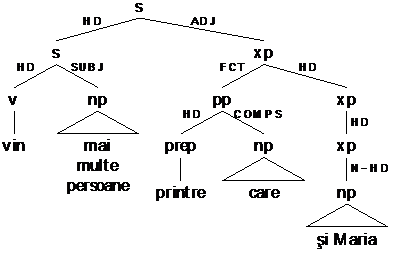
\includegraphics[width=\textwidth]{figures/chap3andconclusion16fevr17-img19.png}
\caption{Syntaxe simplifiée des constructions avec RSV en roumain}
\label{ch3:fig10}
\end{figure}

\ea \label{ch3:ex133}
\gll Vin  mai  multe  persoane,  [\textbf{printre} \textbf{care}  şi  Maria].\\
venir.\textsc{prs.3pl}  plus  beaucoup.\textsc{adj} personnes  parmi  lesquelles  aussi  Maria\\
\glt ‘Plusieurs personnes viennent, parmi lesquelles Maria.’  
\z

La relation syntaxique qui s’établit entre la RSV et la phrase hôte~définit un syntagme de type tête-ajout (\textit{hd-adj-ph}). La relation syntaxique qui existe entre le corps de la RSV et l’introducteur définit un syntagme de type tête-foncteur (\textit{hd-funct-ph}). 


\subsection{Théorie de la localité de sélection sémantique}\label{ch3:sect3.5.4}

Les propriétés de sélection de la RSV et les propriétés de sélection de l’introducteur obéissent au même type de \isi{contraintes de localité}. Plus précisément, il y a deux relations faisant intervenir un problème de localité de sélection : (i) la relation à distance entre la RSV et son antécédent, et (ii) la relation à distance entre l’introducteur et l’élément distingué. Concernant la première relation, si la RSV modifie une phrase, l’antécédent doit être un dépendant direct de la tête de la phrase (comparer les exemples \REF{ch3:ex134b} et \REF{ch3:ex134d}). Concernant la deuxième relation, si l’introducteur modifie un \isi{cluster}, le syntagme exprimant la sous-partie de l’entité fractionnable ({\cad} l’élément distingué) doit être un constituant immédiat du \isi{cluster}, cf. \REF{ch3:ex135}. On observe donc que, dans les deux cas, les contraintes sont du même ordre : soit il y a localité, soit le niveau d’enchâssement est limité à 1.

\ea \label{ch3:ex134}
\ea 
Plusieurs personnes, [\textbf{dont} Marie], sont venues. \label{ch3:ex134a} 
\ex
Plusieurs personnes sont venues, [\textbf{dont} Marie]. \label{ch3:ex134b}
\ex 
Des représentants de plusieurs pays, [\textbf{dont} le Brésil], se sont réunis hier. \label{ch3:ex134c}
\ex 
*Des représentants de plusieurs pays se sont réunis hier, [\textbf{dont} le Brésil]. \label{ch3:ex134d}
\z 
\z

\ea \label{ch3:ex135} 
\ea 
Plusieurs personnes sont venues, [\textbf{dont} Marie]. 
\ex 
Plusieurs personnes sont venues, [\textbf{dont} hier le frère de Marie].
\z 
\z 

Pour formaliser ces \isi{contraintes de localité}, on utilise un dispositif analogue à celui utilisé par \citet{Kiss2005} pour la relation de sélection sémantique à distance entre les subordonnées relatives \is{extraposition}extraposées et leur antécédent en \ili{allemand}. De manière générale, ce mécanisme permet aux ajouts (phrastiques) de modifier des syntagmes dont les propriétés sont très variables, à condition qu’ils contiennent un élément particulier qui puisse être qualifié d’antécédent et que celui-ci ne soit pas trop enchâssé. 

On reprend le trait ANCHORS (dont la valeur est une liste) introduit par \citet{Kiss2005}. Ce trait contient les indices des entités sémantiques qui sont accessibles à la sélection opérée par l’ajout. Les expressions linguistiques introduisent des ancres sémantiques typées qui sont propagées selon certaines règles et sélectionnables. 

Les deux contraintes dont on a besoin pour la propagation d’ancres figurent en \REF{ch3:ex136} et \REF{ch3:ex137}. 

\ea \label{ch3:ex136}
Contrainte de localité 1\\
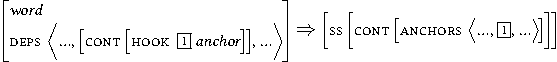
\includegraphics{figures/Ch3136.pdf}

% \noindent 
% \begin{avm}
% [\tp{word}\\
%  deps & <..., [cont [hook & @1 anchor]], ...>]
% \end{avm}
% $\Rightarrow$
% \begin{avm}
% [ss [cont [anchors & <..., @1, ...>]]]
% \end{avm}

\z


\ea \label{ch3:ex137}
Contrainte de localité 2\\
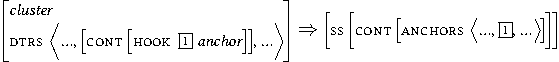
\includegraphics{figures/Ch3137.pdf}

% \noindent 
% \begin{avm}
% [\tp{cluster}\\
%  dtrs & <..., [cont [hook & @1 anchor]], ...>]
% \end{avm}
% $\Rightarrow$
% \begin{avm}
% [ss [cont [anchors & <..., @1, ...>]]]
% \end{avm}

\z

La première contrainte donnée en \REF{ch3:ex136} dit qu’au niveau d’un syntagme tous les dépendants directs de la tête sont sélectionnables et accessibles via l’ensemble des ancres.

La deuxième contrainte définie en \REF{ch3:ex137} garantit qu’au niveau d’un \isi{cluster} tous les constituants immédiats du \isi{cluster} sont sélectionnables et accessibles via l’ensemble des ancres. Un autre avantage des contraintes d’ancre est qu’elles restreignent la sélection sémantique au matériel qui est littéralement introduit dans le \isi{cluster}. Les relations sémantiques reconstruites ne sont donc pas disponibles pour la sélection sémantique.

Le résultat de l’application de ces deux contraintes sur une RSV sera donné plus tard, une fois qu’on aura introduit tous les éléments nécéssaires pour l’analyse.


\subsection{Théorie des RSV}\label{ch3:sect3.5.5}

Cette section fait la synthèse des contraintes syntaxiques et sémantiques qui s’appliquent à la RSV dans son ensemble et montre la manière dont elles interagissent.  
Les contraintes syntaxiques dans les RSV dérivent : (i) des propriétés des \is{cluster}clusters, (ii) des propriétés de sélection des introducteurs, et (iii) des propriétés cons\-tructionnelles des RSV. Les \is{cluster}clusters ont des propriétés inhérentes qui peuvent entrer en conflit avec les propriétés des RSV. Par exemple, les syntagmes dans un \isi{cluster} doivent être des dépendants directs de la tête de la phrase hôte et avoir le même marquage que les syntagmes parallèles dans l’hôte. Cette contrainte entrera en conflit avec les propriétés de sélection de certains introducteurs, comme \textit{parmi lesquel(le)s} en français, qui contraignent le syntagme exprimant la sous-partie ({\cad} l’élément distingué) à être un syntagme nominal non marqué \REF{ch3:ex138}.

\ea \label{ch3:ex138}
\ea 
J’ai parlé à plusieurs personnes, [\textbf{dont} à Marie de linguistique]. 
\ex
*J’ai parlé à plusieurs personnes, [\textbf{parmi lesquelles} à Marie de linguistique].
\z 
\z 

Les propriétés constructionnelles de la RSV dans son ensemble incluent la présence d’un introducteur avec une sémantique partitive. Pour les RSV introduites par un syntagme \textit{qu-}, il doit être précisé que l’introducteur doit contenir une forme \textit{qu-} \is{coréférence}coréférentielle avec l’antécédent dans la phrase hôte.

Les contraintes sémantiques des RSV dérivent : (i) de la sémantique du \isi{fragment}, et (ii) de la sémantique partitive des RSV. Les RSV ont un type de contenu similaire à celui d’une phrase. Elles se comportent comme des \is{anaphore descriptive}anaphores descriptives, par le fait qu’elles introduisent une nouvelle entité sémantique qui partage une partie de sa description avec l’antécédent. Dans le cas des RSV, cette nouvelle entité est une sous-éventualité. Les RSV introduisent simultanément deux relations partitives : la première relation partitive relie l’antécédent et une nouvelle entité introduite par un syntagme dans le corps de la RSV. Cette relation est exprimée par l’introducteur. Cela est mis en évidence par le fait que les RSV peuvent avoir soit une \isi{interprétation exemplifiante}, soit une \isi{interprétation partitionnante}, mais tous les introducteurs ne sont pas compatibles avec les deux interprétations. La deuxième relation partitive relie \is{éventualité}l’éventualité dénotée par la phrase source et la sous-éventualité introduite par la RSV.

La RSV est définie en \REF{ch3:ex139}. La tête du syntagme est un \isi{fragment} phrastique. Il est sélectionné par l’introducteur de la RSV imposant une relation ensemble/sous-partie (\textit{sum-subpart-rel}), relation sémantique qui est caractéristique de cette cons\-truction. La relation ensemble/sous-partie est supposée avoir deux sous-types : un sous-type exemplifiant (\textit{exemplifying-sum-subpart-rel}) et un sous-type partitionnant (\textit{partitioning-sum-subpart-rel}). La construction elle-même apporte une deu\-xième relation mettant en jeu une sous-partie : on met ainsi en relation \is{éventualité}l’éven\-tualité dénotée par la phrase hôte [SUM \fbox{6} \textit{event}], avec \is{éventualité}l’éventualité dénotée par le \isi{fragment} phrastique [SUBPART \fbox{7} \textit{event}]. De plus, la construction sélectionne un antécédent nominal. On note aussi l’emploi de la liste ANCHORS pour exprimer la localité de la sélection opérée par l’introducteur et par la RSV elle-même. Ainsi, [ANCHORS <..., [IND \fbox{10}], ...>] nous permet d’avoir accès à l’antécédent, qui désigne une \isi{entité plurielle} [SUM \fbox{10}] dans la phrase hôte, alors que [ANCHORS <..., [IND \fbox{8}], ...>] nous permet l’accès à l’élément distingué, qui dénote la sous-partie [SUBPART \fbox{8}] dans le corps de la RSV. Enfin, il faut rappeler que les contraintes sémantiques données en \REF{ch3:ex116} ci-dessus s’appliquent à toute construction RSV.

\ea \label{ch3:ex139}
La construction RSV\footnote{Comme toutes les étiquettes utilisées dans les représentations arborescentes et les matrices attribut-valeur en HPSG sont en anglais, on va utiliser l’étiquette anglaise VRA (\textit{Verbless Relative Adjuncts}) au lieu de l’étiquette française RSV.}\\
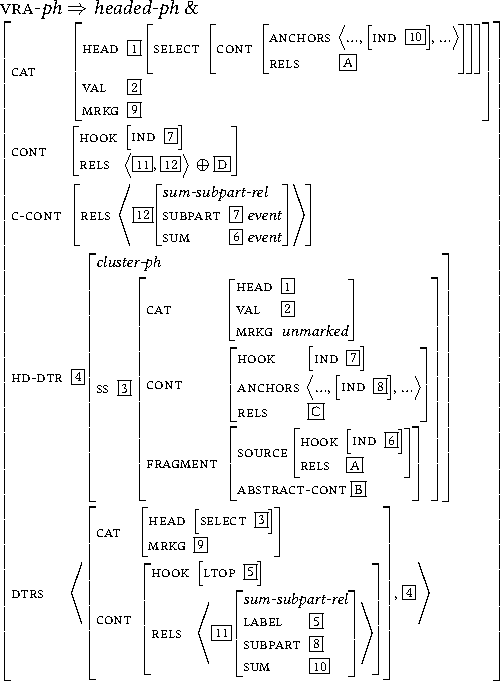
\includegraphics{figures/Ch3139.pdf}

% \noindent
% \textsc{vra}-\textit{ph} $\Rightarrow$ \textit{headed-ph} \& \\
% \begin{avm} 
% [cat & [head & @{1} [select & [cont &    [anchors &  <..., [ind & @{10}], ...> \\ rels & @{A} ]]]\\
% 									  val & @{2}\\
% 									  mrkg & @{9}]\\
% 						 cont & [hook & [ind & @{7}] \\ rels & <@{11}, @{12}> & $\oplus$ @{D}]\\
% 						 c-cont & [rels & <@{12}[\tp{sum-subpart-rel}\\
% 							 										subpart & @{7} event\\
% 							 										sum & @{6} event]>]\\
% hd-dtr & @{4}[\tp{cluster-ph}\\ ss & @{3} [cat & [head & @{1}\\
% 																	val & @{2}\\
% 																	mrkg & unmarked]\\
% 													 cont & [hook & [ind & @{7}]\\
% 																				anchors & <..., [ind & @{8}], ...> \\ rels & @{C}]\\
% 													 fragment & [source [hook & [ind & @{6}] \\ rels & @{A}]\\
% 													  						abstract-cont  @{B}]\\
% 									 ]\\
% 									 ]\\
% dtrs & <[cat & [head & [select & @3] \\ mrkg & @{9}]\\
% 	      cont & [hook & [ltop & @{5}]\\
% 								rels & < @{11}[\tp{sum-subpart-rel}\\
% 												label & @{5}\\
% 												subpart & @{8}\\
% 							 					sum & @{10}]>]], @{4}>]
													
% \end{avm}	

\z

Selon la forme de l’introducteur, la construction RSV a deux sous-types : une RSV dont l’introducteur contient un mot \textit{qu-} (\textit{WH-VRA-ph}) et une RSV (en français uniquement) dont l’introducteur est \textit{dont} (\textit{DONT-VRA-ph}).

En ce qui concerne le premier sous-type (\textit{WH-VRA-ph}) défini en \REF{ch3:ex140}, l’introducteur contient une forme \textit{qu-} qui est \is{coréférence}coréférentielle avec l’antécédent nominal dans la phrase hôte (cf. le partage d’indices).

\ea \label{ch3:ex140}
La construction RSV avec un introducteur contenant une forme \textit{qu-}\\
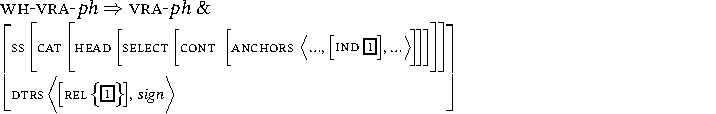
\includegraphics{figures/Ch3140.pdf}

% \noindent
% \textsc{wh}-\textsc{vra}-\textit{ph} $\Rightarrow$ \textsc{vra}-\textit{ph} \& \\
% \begin{avm}
% [ss [cat [head [select [cont & [anchors & <..., [\textsc{ind} @1], ...>]]]]]\\
%  dtrs <[rel \{@1\}], \textit{sign}>] 
% \end{avm}

\z

Les prépositions fonctionnant comme tête dans l’introducteur de la RSV (p.ex. roum. \textit{dintre, printre, între} et fr. \textit{parmi}) ont les propriétés lexicales suivantes : elles ont une structure argumentale qui contient deux éléments, un argument interne (qui est un pronom relatif) réalisé comme complément (COMPS) de la préposition et un argument externe (XARG) qui n’est pas réalisé comme dépendant de la préposition. La préposition sélectionne un syntagme qui contient une ancre coïndicée avec son argument externe. La préposition doit aussi introduire une relation ensemble/sous-partie (\textit{sum-subpart-rel}) entre ses deux arguments : l’argument interne dénote l’ensemble (SUM), alors que l’argument externe dénote la sous-partie (SUBPART) de l’ensemble. Les prépositions peuvent différer selon qu’elles permettent les deux types d’interprétation discutés dans la section~\ref{ch3:sect3.3.2.2}, à savoir une \isi{interprétation exemplifiante} et une \isi{interprétation partitionnante}, ou bien uniquement une de ces deux interprétations. Ainsi, la préposition \textit{dintre} en roumain \REF{ch3:ex143} est compatible uniquement avec une \isi{interprétation partitionnante}, alors que les autres prépositions (roum. \textit{printre} et \textit{între} \REF{ch3:ex144} et fr. \textit{parmi} \REF{ch3:ex145}) introduisent une relation sous-spécifiée ({\cad} elles sont compatibles avec les deux interprétations). 

Enfin, les prépositions peuvent contraindre la catégorie du corps de la RSV via le trait SELECT. Ainsi, la préposition \textit{dintre} en roumain \REF{ch3:ex143} n’est compatible qu’avec un syntagme nominal non marqué (le cas de l’élément distingué dans le corps de la RSV doit être direct, {\cad} il doit avoir une forme de nominatif-accusatif, et non de datif-génitif, comme illustré en \REF{ch3:ex141}), alors que la préposition \textit{printre} ou \textit{între} en roumain \REF{ch3:ex144} ne contraint pas la catégorie du corps de la RSV. En français, la préposition \textit{parmi} \REF{ch3:ex145} contraint le corps de la RSV à contenir un syntagme nominal non marqué par une préposition \REF{ch3:ex142}. 

\ea \label{ch3:ex141}
\gll Impactul  a  dus  la  spitalizarea  mai  multor  persoane, [\textbf{dintre} \textbf{care}  (*\uline{a})  şapte  români].\\
impact.\textsc{def}  a  mené  à  hospitalisation.\textsc{def}  plus  beaucoup.\textsc{adj.gen}  personnes parmi  lesquelles  (\textsc{gen.sg.f)}  sept  Roumains\\
\glt ‘L’impact a mené à l’hospitalisation de plusieurs personnes, dont sept Roumains.’
\z 

\ea \label{ch3:ex142}
J’ai parlé \textbf{à} plusieurs personnes, [\textbf{parmi lesquelles} (*\uline{à}) Marie].
\z

\ea \label{ch3:ex143}
Entrée lexicale pour la préposition \textit{dintre} en roumain\\
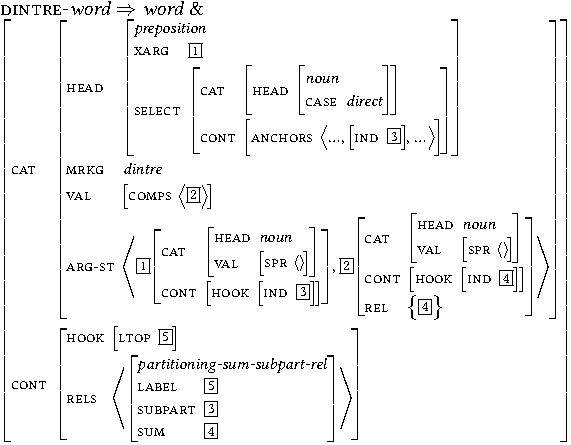
\includegraphics{figures/Ch3143.pdf}

% \noindent
% \textsc{dintre}-\textit{word} $\Rightarrow$ \textit{word} \& \\
% \begin{avm}
% [cat & [head & [\tp{preposition}\\
% 								xarg & @{1}\\
% 								select & [cat & [head & [\tp{noun}\\
% 																 case & direct]]\\
% 										cont & [anchors & <..., [ind & @{3}], ...>]]]\\
% 				mrkg & dintre \\
% 				val & [comps & <@{2}>]\\
% 				arg-st & <@{1}[cat & [head & noun\\
% 														  val & [spr & <>]]\\
% 											 cont & [hook &[ind & @{3}]]], @{2}[cat & [head & noun\\
% 														  																	 val & [spr & <>]]\\
% 											 																		cont & [hook &[ind & @{4}]]\\
% 																													rel & \{@{4}\}]>]\\
% cont & [hook & [ltop & @{5}]\\
% 				rels & <[\tp{partitioning-sum-subpart-rel}\\
%                  label & @{5}\\
%                  subpart & @{3}\\
%                  sum & @{4}]>]]
% \end{avm}

\z


\ea \label{ch3:ex144}
Entrée lexicale pour la préposition \textit{printre} en roumain (de même pour \textit{între})\\
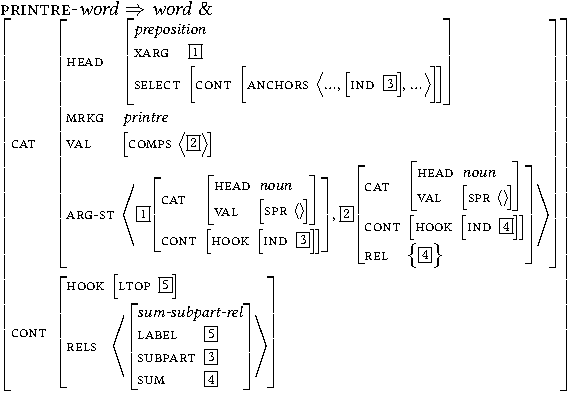
\includegraphics{figures/Ch3144.pdf}

% \noindent 
% \textsc{printre}-\textit{word} $\Rightarrow$ \textit{word} \& \\
% \begin{avm}
% [cat & [head & [\tp{preposition}\\
% 								xarg & @{1}\\
% 								select & [cont & [anchors & <..., [ind & @{3}], ...>]]]\\
% 				mrkg & printre \\
% 				val & [comps & <@{2}>]\\
% 				arg-st & <@{1}[cat & [head & noun\\
% 														  val & [spr & <>]]\\
% 											 cont & [hook &[ind & @{3}]]], @{2}[cat & [head & noun\\
% 														  																	 val & [spr & <>]]\\
% 											 																		cont & [hook &[ind & @{4}]]\\															rel & \{@{4}\}]>]\\							
% cont & [hook & [ltop & @{5}]\\
% 				rels & <[\tp{sum-subpart-rel}\\
%                  label & @{5}\\
%                  subpart & @{3}\\
%                  sum & @{4}]>]]
% \end{avm}

\z


\newpage 
\ea \label{ch3:ex145}
Entrée lexicale pour la préposition \textit{parmi} en français\\
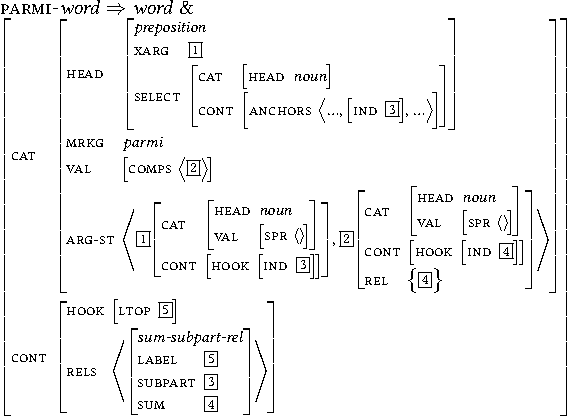
\includegraphics{figures/Ch3145.pdf} 
\z

\begin{figure}
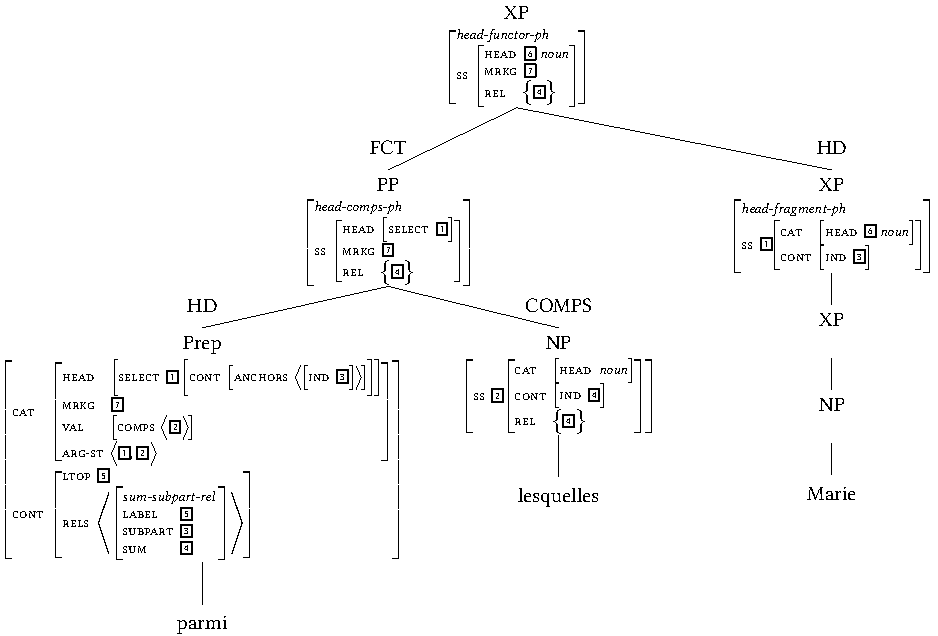
\includegraphics[width=\textwidth]{figures/Ch3Fig11.pdf}  
\caption{Relation à distance entre l’introducteur et l’élément distingué}
\label{ch3:fig11}
\end{figure}



Une exemplification de cette analyse est donnée en \figref{ch3:fig11}. La préposition \textit{parmi} en français introduit une relation partitive sous-spécifiée (\textit{sum-subpart-rel}), {\cad} elle est compatible et avec \is{interprétation exemplifiante}l’interprétation exemplifiante et aussi avec \is{interprétation partitionnante}l’inter\-prétation partitionnante. Sa structure argumentale contient un argument externe (qui dénote la sous-partie et qui correspond donc au syntagme \textit{Marie}) et un complément (qui dénote l’ensemble et qui correspond donc au pronom relatif \textit{lesquelles}). Cette représentation exemplifie aussi le résultat de l’application d’une des deux \isi{contraintes de localité} discutées plus haut dans la section~\ref{ch3:sect3.5.4}, à savoir la relation à distance entre l’introducteur et l’élément distingué : l’élément distingué dans le corps de la RSV est rendu accessible via le trait ANCHORS.

\begin{figure}[b]
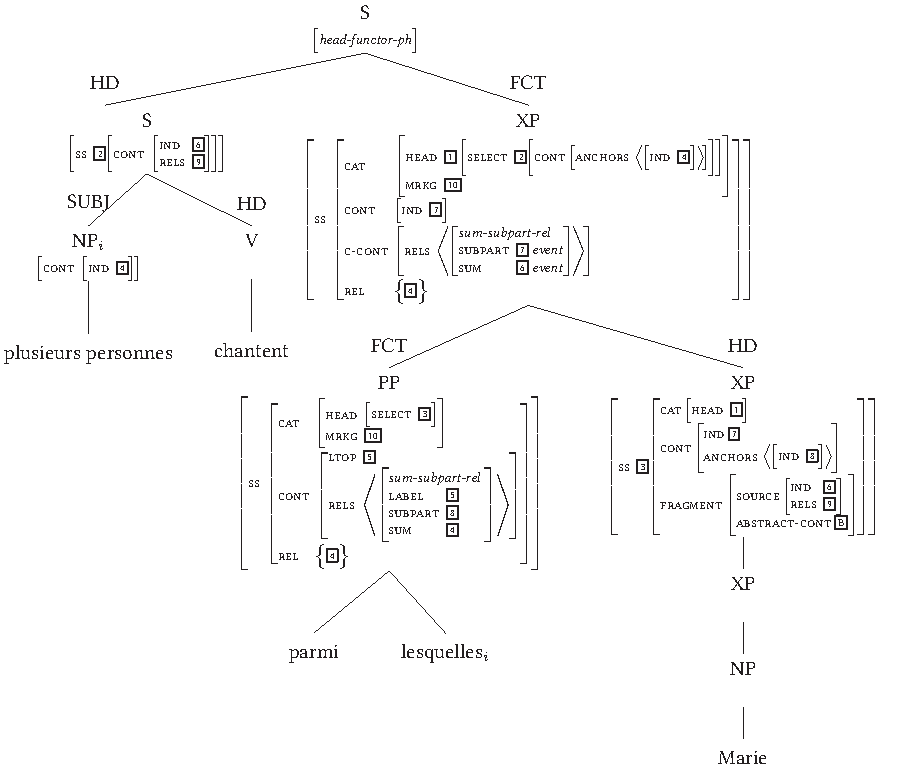
\includegraphics[width=\textwidth]{figures/Ch3Fig12.pdf}  
\caption{Relation à distance entre la RSV et son antécédent}
\label{ch3:fig12}
\end{figure}

En \figref{ch3:fig12}, on a une représentation simplifiée de la construction dans son ensemble, qui nous permet d’observer aussi le résultat de l’application de la deu\-xième \is{contraintes de localité}contrainte de localité discutée dans la section~\ref{ch3:sect3.5.4}, à savoir la relation à distance entre la RSV et son antécédent dans la phrase hôte : l’antécédent (ici, le syntagme nominal \textit{plusieurs personnes}, qui est coïndicé avec le pronom relatif \textit{lesquelles}) est rendu accessible à la RSV via le trait ANCHORS. 



En ce qui concerne le deuxième sous-type de RSV (\textit{DONT-VRA-ph}) défini en \REF{ch3:ex146}, il aura comme seule contrainte le fait que le nœud racine de la construction possède un trait MARKING (abrégé MRKG) dont la valeur est \textit{dont}.

  
\ea \label{ch3:ex146}
La construction RSV avec un introducteur contenant \textit{dont} en français\\
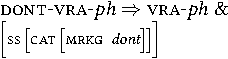
\includegraphics{figures/Ch3146.pdf}

% \noindent 
% \textsc{dont}-\textsc{vra}-\textit{ph} $\Rightarrow$ \textsc{vra}-\textit{ph} \& \\
% \begin{avm}
% [ss [cat [mrkg & dont]]] 
% \end{avm}

\z

On analyse le français \textit{dont} comme un marqueur qui n’a pas de structure argumentale, introduisant une relation sémantique sous-spécifiée. \textit{Dont} sélectionne un syntagme qui (i) contient une ancre pour l’argument dénotant la sous-partie et (ii) sélectionne un syntagme contenant une ancre pour l’argument dénotant l’ensemble. L’entrée lexicale pour la forme \textit{dont} dans les RSV est donnée en \REF{ch3:ex147}. Ainsi, [ANCHORS <..., [IND \fbox{4}], ...>] nous permet d’avoir accès à l’antécédent, qui désigne une entité plurielle [SUM \fbox{4}] dans la phrase hôte, alors que [ANCHORS <..., [IND \fbox{3}], ...>] nous permet l’accès à l’élément distingué, qui dénote la sous-partie [SUBPART \fbox{3}] dans le corps de la RSV. 

\ea \label{ch3:ex147}
Entrée lexicale pour \textit{dont} dans les RSV en français\\
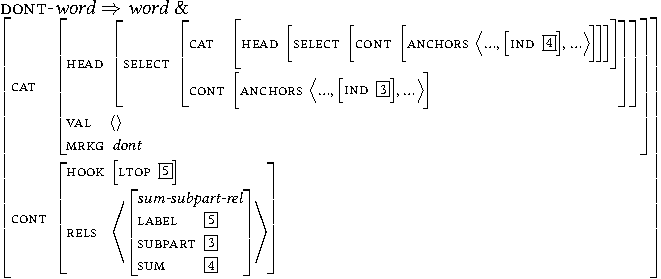
\includegraphics{figures/Ch3147.pdf}

% \noindent 
% \textsc{dont}-\textit{word} $\Rightarrow$ \textit{word} \& \\
% \begin{avm}
% [cat & [head & [select & [cat & [head & [select & [cont & [anchors & <..., [ind & @{4}], ...>]]]]\\
% 													cont & [anchors & <..., [ind & @{3}], ...>]]]\\
% 				val & <>\\
% 				mrkg & dont]\\
% cont & [hook & [ltop & @{5}]\\
% 				rels & <[\tp{sum-subpart-rel}\\
%                  label & @{5}\\
%                  subpart & @{3}\\
%                  sum & @{4}]>]]
% \end{avm}

\z

L’entrée proposée en \REF{ch3:ex146} pour l’introducteur \textit{dont} dans les RSV est différente de celle postulée pour le complémenteur \textit{dont} dans les relatives verbales en français \citep{Godard1988,Godard1989,AbeilleEtAl2003c,AbeilleEtAl2006,AbeilleEtAl2007}. Le complémenteur\footnote{ \citet{Sag1997} définit un super-type \textit{verbal} qui a comme sous-types le verbe et les complémenteurs.} \textit{dont} est défini en \REF{ch3:ex148}.

\ea \label{ch3:ex148}
Entrée lexicale pour le complémenteur \textit{dont} dans les relatives ordinaires\\
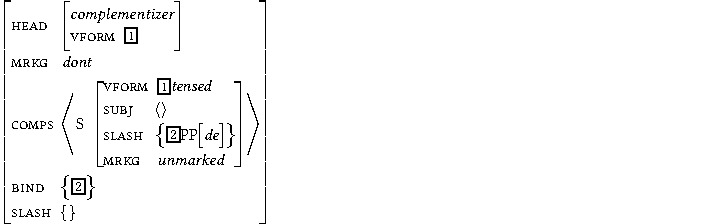
\includegraphics{figures/Ch3148.pdf}

% \noindent 
% \begin{avm}
% [head & [\tp{complementizer}\\
% 				 vform & @{1}]\\
% mrkg & dont\\
% comps & <S & [vform & @{1}tensed\\
% 							subj & <>\\
% 							slash & \{@{2}PP[\textit{de}]\}\\
% 							mrkg & unmarked]>\\
% bind & \{@{2}\}\\ 
% slash & \{\}]
% \end{avm} 

\z

Contrairement à l’introducteur \textit{dont} dans les RSV, le complémenteur \textit{dont} est une tête syntaxique\footnote{Plus précisément, on peut considérer que le complémenteur \textit{dont} est une \is{tête faible}tête «~faible~», {\cad} une tête syntaxique qui partage sa valeur de HEAD avec son complément (cf. \citealt{Tseng2002}).}, prenant comme complément une phrase tensée\footnote{ Pour les phrases verbales en français, on peut faire la distinction entre phrase tensée et phrase finie \citep{GGFToAppear}. Une phrase tensée contient nécessairement une forme verbale ayant une marque de temps (indicatif, subjonctif, etc.). En revanche, l’opposition fini/non-fini est pertinente en français à cause du placement de la \isi{négation} : les participes présents se distinguent des infinitifs, cf. \textit{ne venant pas} vs. \textit{*ne venir pas}. On peut ainsi considérer l’infinitif comme une forme verbale non finie et non tensée et le participe présent comme une forme finie et non tensée. Le complémenteur \textit{dont} n’est compatible qu’avec une phrase tensée en français.},~auquel manque un constituant prépositionnel. En français standard, ce gap est un syntagme prépositionnel en \textit{de}. Le trait BIND sert à lier la valeur du trait SLASH du complément phrastique. Comme la valeur est un syntagme prépositionnel en \textit{de}, le gap dans une relative standard en \textit{dont} est toujours un syntagme prépositionnel.

Je donne en \figref{ch3:fig13} un exemple de relative verbale introduite par le complémenteur \textit{dont}. Le verbe \textit{parle} possède un trait SLASH non vide indiquant qu’un argument est manquant. Le trait SLASH est partagé par les catégories dominant le verbe jusqu’à la relative elle-même, qui le «~vide~». 


En revanche, une RSV en \textit{dont} n’a pas de trait SLASH, car il n’y a pas de constituant manquant. Je donne en \figref{ch3:fig14} un exemple de RSV en \textit{dont}. 

\newpage  
% \largerpage[10]
\begin{figure}
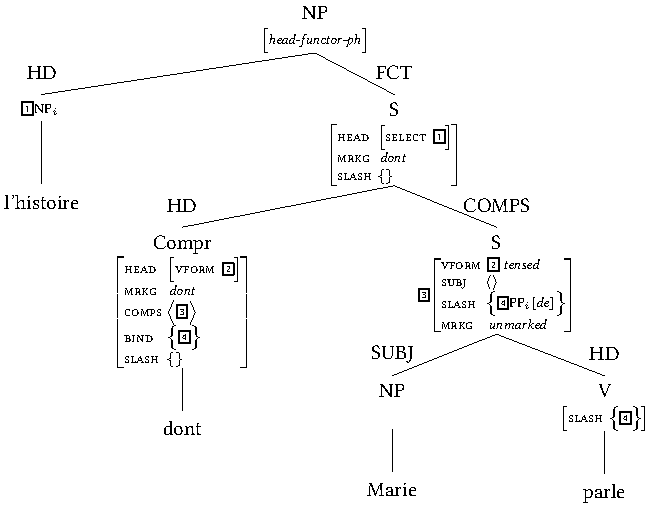
\includegraphics[height=.29\textheight]{figures/Ch3Fig13.pdf}  
\caption{Arbre avec le complémenteur \textit{dont} dans les relatives verbales ordinaires}
\label{ch3:fig13}
\end{figure}

~
\begin{figure}
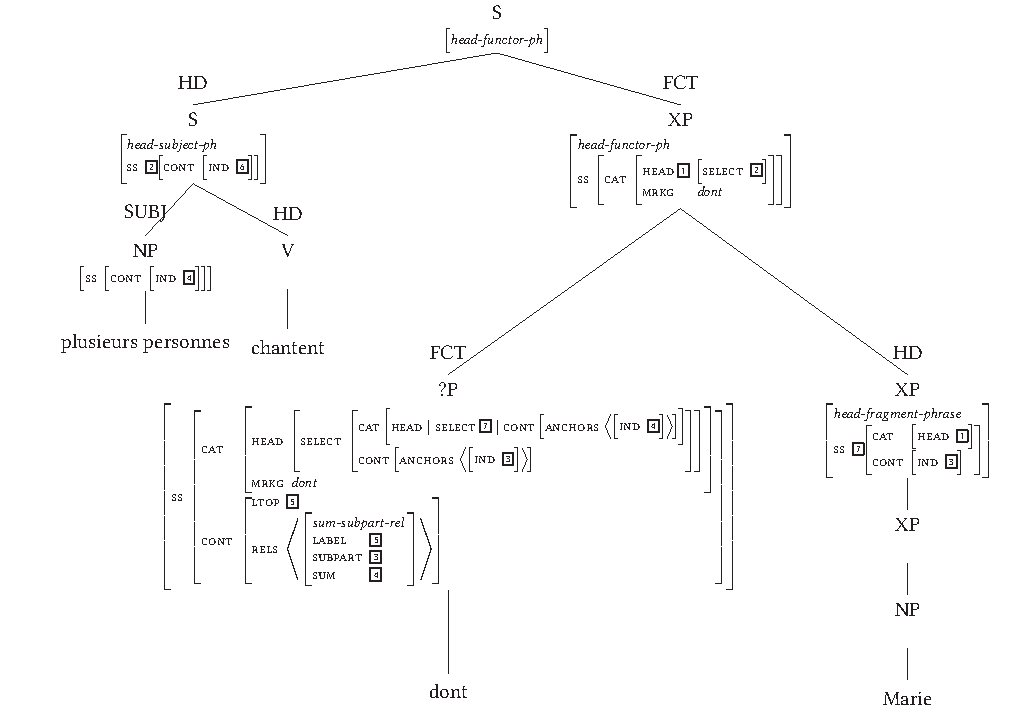
\includegraphics[width=\textwidth]{figures/Ch3Fig14.pdf}  
\caption{Arbre avec l’introducteur \textit{dont} dans les RSV}
\label{ch3:fig14}
\end{figure}

\clearpage   
\section{Conclusion}\label{ch3:sect3.6}

Les RSV se caractérisent par les propriétés suivantes : (i) ce sont des \is{ajout incident}ajouts incidents ; (ii) elles ont une sémantique non restrictive, bien qu’elles fassent partie du contenu asserté de l’hôte, et (iii) elles ont une double sémantique partitive : au niveau des individus et au niveau des \is{éventualité}éventualités. En fonction du statut de l’élément distingué par rapport à l’antécédent, cette relation partitive se prête à deux interprétations : une \isi{interprétation exemplifiante} si l’élément distingué constitue un élément de l’ensemble dénoté par l’antécédent, ou bien une \isi{interprétation partitionnante} si l’élément distingué constitue un sous-ensemble de l’ensemble dénoté par l’antécédent. 


Les RSV en roumain et en français ont été décrites comme des phrases relatives présentant une ellipse du verbe, en vertu de leur ressemblance avec les phrases relatives partitives non restrictives. Bien qu’une analyse en termes de \isi{reconstruction syntaxique} puisse rendre compte de certaines propriétés des RSV, on a présenté des arguments empiriques (provenant des deux langues) contre une telle approche. 


Une analyse des RSV comme des ajouts fragmentaires rend compte de l’ensemble des propriétés des RSV. Bien que cette nouvelle approche puisse sembler techniquement complexe, les parties individuelles qui la composent sont justifiées de manière indépendante pour d’autres constructions dans la grammaire des deux langues.  